\documentclass[14pt]{extarticle}

\usepackage{geometry}
\geometry{a4paper,
          total={165mm,257mm},
          left=30mm,
          top=20mm,
         }

\usepackage{cmap}

\usepackage[utf8]{inputenc}
\usepackage[T1, T2A]{fontenc}
\usepackage[english, russian]{babel}
\usepackage{csquotes}

% \usepackage[
%     backend = biber,
%     style = numeric,
% ]{biblatex}

% \addbibresource{Refs.bib}

\usepackage{graphicx}
\graphicspath{ {./images/} }

\usepackage{subcaption}

% \usepackage{amsmath}


\title{Изучение влияния напряжений $U_1$ и $U_R$ на форму частотных 
сканов транзисторов КТ117Б}
\author{Богачев А.М.}
\date{\today}


\begin{document}

    \maketitle
    \begin{abstract}
        В отчёте приведены результаты измерений, целью которых было
        изучение влияния напряжений $U_1$ и $U_r$ на форму частотных 
        сканов. Объект исследования -- p-n-переходы транзистора 
        КТ117Б~№1. Зафиксированны частотные сканы для всех возможных пар
        значений $U_1$ (от -1~В до -11~В) и $U_R$ (от -2~В до -12~В). 
        Измерения проводились при трёх значениях температуры: 263~К, 
        283~К и 303~К. Идентифицированны параметры моделей чачтотных 
        сканов. В отчёте приведены графики экспериментальных данных, 
        графики с результатами идентификации параметров моделей частотных 
        сканов и графики зависимости коэффициента $p$ от различных 
        значений разности $U_R - U_1$ для каждой из температур.
    \end{abstract}

    \section{Введение}

\emph{Цель исследования}: регистрация частотных сканов p-n-переходов 
транзистора КТ117Б, подключенного как показано на рисунке~\ref{pic:installation}. 
Изучение влияния напряжений $U_1$ и $U_r$ на форму частотных сканов.
\begin{figure}[!ht]
	\centering
	\begin{subfigure}[t]{0.45\textwidth}
		\centering
		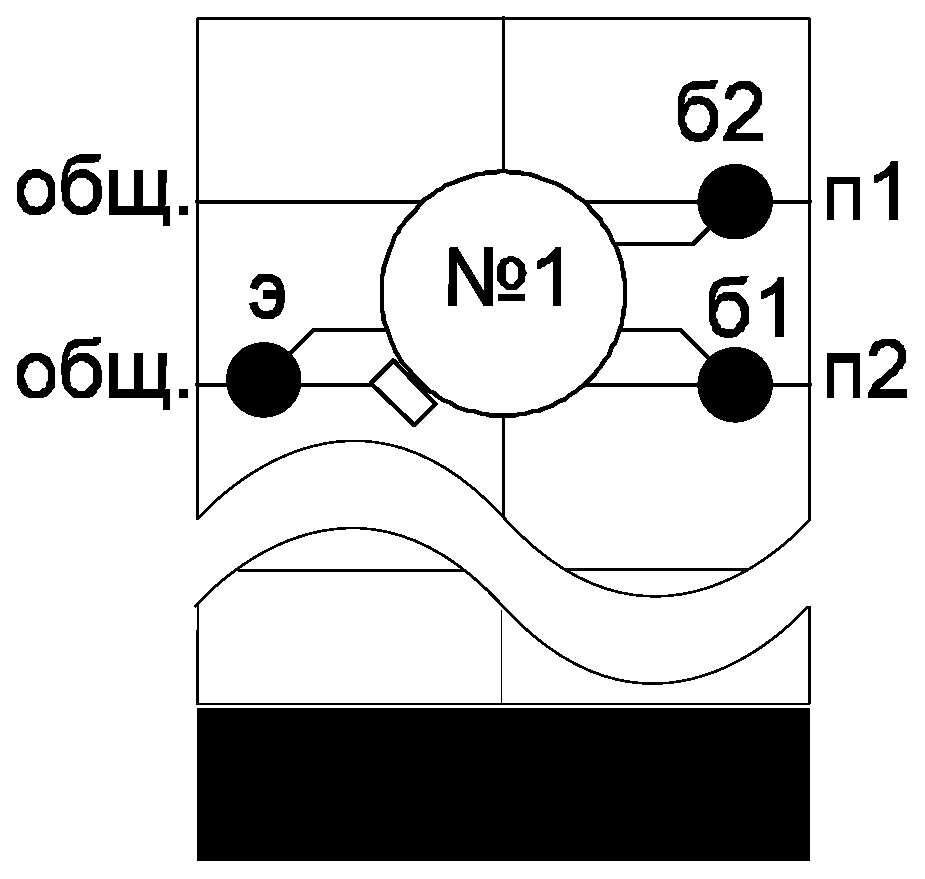
\includegraphics[width=0.6\linewidth]{pic1-install}
		\caption{Схема установки транзисторов в контактирующее
		приспособление. Транзисторы показаны выводами вниз.}
	\end{subfigure}
	\begin{subfigure}[t]{0.45\textwidth}
		\centering
		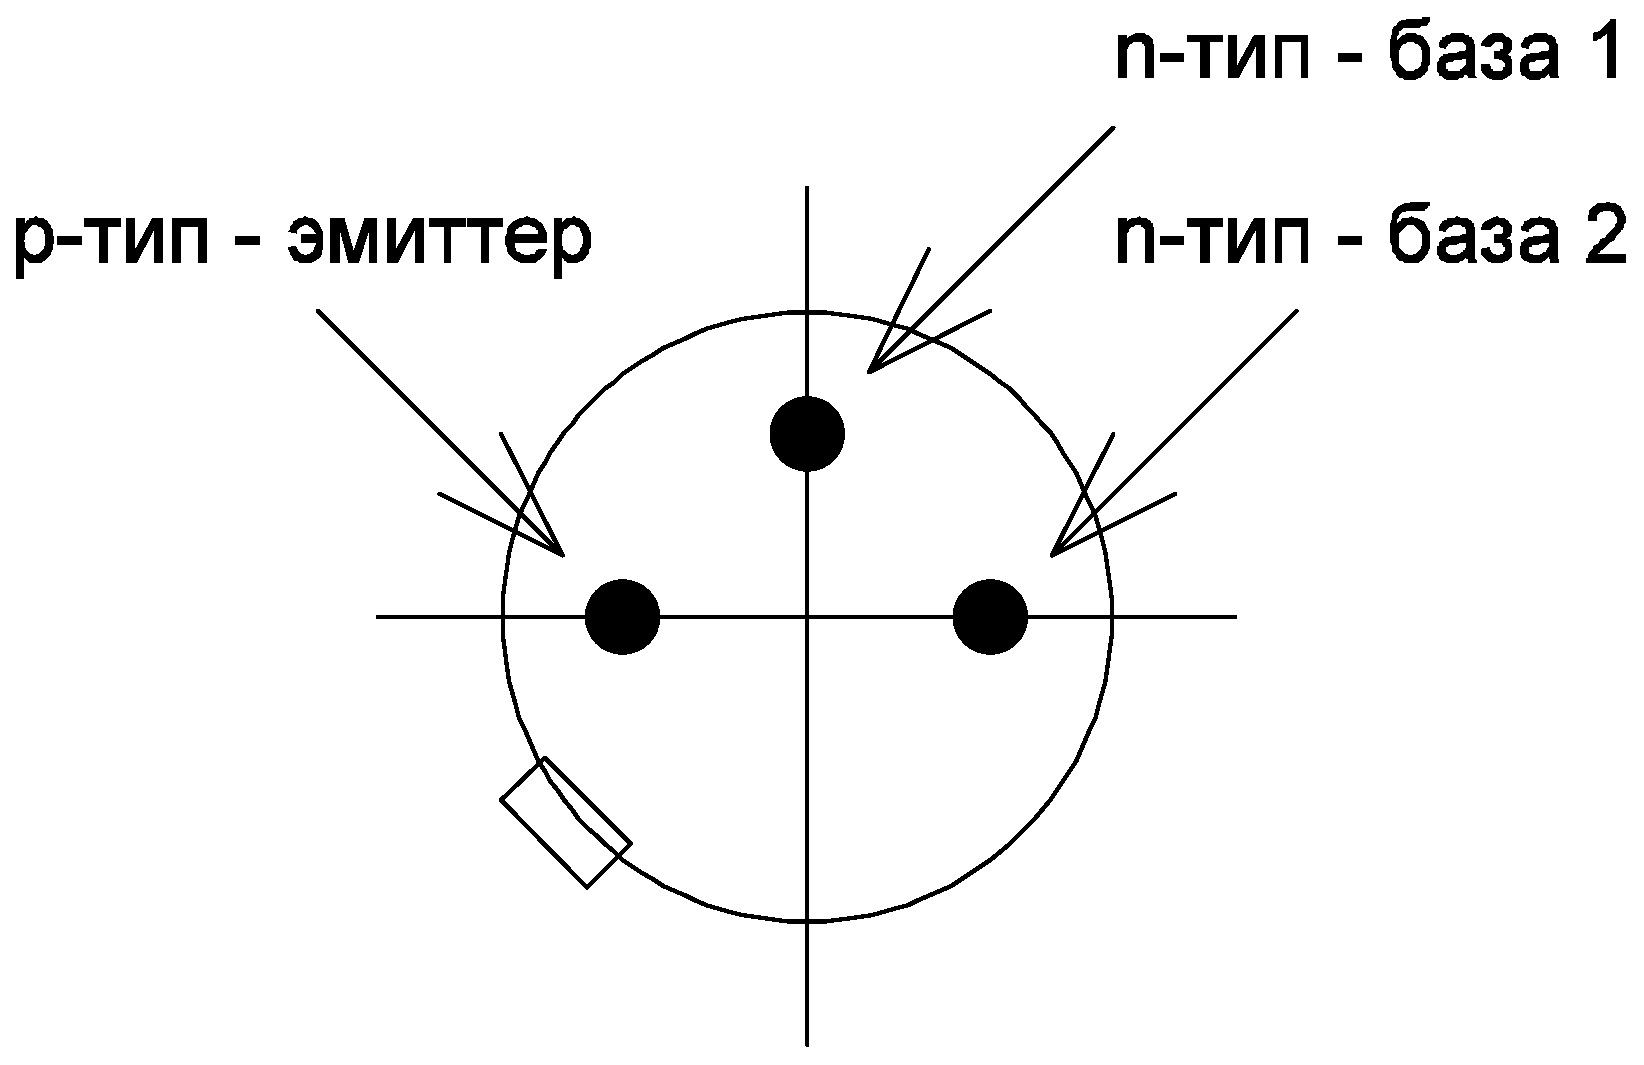
\includegraphics[width=0.9\linewidth]{pic1-pins}
		\caption{Расположение контактов транзистора КТ117Б. Транзистор
		показан выводами вверх.}
	\end{subfigure}

	\caption{Схема установки транзисторов.}
	\label{pic:installation}
\end{figure}

Условия, одинаковые для всех сканов перечислены в таблице 
\ref{table:common_conditions}.
\begin{table}[!ht]
	\centering
	\caption{Условия, одинаковые для всех сканов.}
	\begin{tabular}{|l|l|}
		\hline
		Параметр                           & Значение             \\ \hline
		Образцы                            & КТ117Б~№1            \\ \hline
		Длительность импульса, мкс         & 20                   \\ \hline
		Автоматическая компенсация моста   & включена             \\ \hline
		Шаг сканирования                   & 0.1                  \\ \hline
		Начальная частота сканирования, Гц & 1                    \\ \hline
		Конечная  частота сканирования, Гц & 2500                 \\ \hline
		Интервал между измерениями, с      & 3.5                  \\ \hline
		Постоянная интегрирования, с       & 3                    \\ \hline
	\end{tabular}
	\label{table:common_conditions}
\end{table}

На рисунке \ref{pic:p_coef_plot} показанны графики со значениями 
коэффициента $p$, соответствующих различным значениями разности $U_R - U_1$,
для трёх значений температуры образца: 263 К, 283 К, 303 К. На графиках 
отображены все пары $U_R$ и $U_1$ одновременно, что может частично 
обуславливать разброс.
\begin{figure}[!ht]
	\centering
	\includegraphics[height=0.95\textheight]{Зависимость_p_от_разности_u1_ur}
	\caption{Значения коэффициента $p$ для различных значений разности $U_R$ и $U_1$.}
	\label{pic:p_coef_plot}
\end{figure}

    %Файл сгенерирован автоматически на основе собранных и обработанных данных


\section{Результаты измерений}
В данном разделе приведены результаты измерений и идентификации параметров полученных сканов.
\subsection{Частотный скан №1}
\begin{table}[!ht]
    \centering
    \caption{Параметры частотного скана №1.}
    \begin{tabular}{|l|l|}
        \hline
        Параметр                                       & Значение                  \\ \hline
        Образец                                        & КТ117№1 п1(база 2)        \\ \hline
        Балансировка моста                             & см. рабочий журнал        \\ \hline
        Чувствительность моста, пФ                     & 1                         \\ \hline
        Чувствительность селектора, мВ                 & 200                       \\ \hline
        $U_R$, В                                       & -12.00                    \\ \hline
        $U_1$, В                                       & -1.00                     \\ \hline
        Температура в лаборатории, $^\circ C$          & см. рабочий журнал        \\ \hline
        Температура образца в начале сканирования, $K$ & 263.22                    \\ \hline
        Температура, установленная на КТХ, $^\circ C$  & см. рабочий журнал        \\ \hline
        Время начала сканирования                      & 11:57:29                  \\ \hline
        Дата                                           & 2022-04-28                \\ \hline
    \end{tabular}
    \label{table:frequency_scan_1}
\end{table}

\begin{table}[!ht]
    \centering
    \caption{Параметры модели частотного скана №1.}
    \begin{tabular}{|l|r|}
        \hline
        Параметр                                       & Значение                  \\ \hline
        $\log_{10}(\tau)$, $\log_{10}$(с)              & -1.629950e+00             \\ \hline
        $\tau$, с                                      & 2.344500e-02              \\ \hline
        $A$, пФ                                        & -9.865870e-03             \\ \hline
        $p$                                            & 7.896081e-01              \\ \hline
        MSE, пФ$^2$                                    & 7.728459e-08              \\ \hline
        RMSE пФ                                        & 2.780011e-04              \\ \hline
    \end{tabular}
    \label{table:frequency_scan_model_1}
\end{table}

\textbf{Имена файлов}

Результаты измерений и параметры модели:

\scriptsize../models/КТ117№1\_п1(база 2)\_2500Гц-1Гц\_1пФ\_-10С\_-1В-12В\_200мВ\_20мкс\_шаг\_0,1\_model.csv
\normalsize

График с результатами измерений:

\scriptsize../plots/КТ117№1\_п1(база 2)\_2500Гц-1Гц\_1пФ\_-10С\_-1В-12В\_200мВ\_20мкс\_шаг\_0,1.pdf
\normalsize

График с результатами идентификации модели:

\scriptsize../plots/КТ117№1\_п1(база 2)\_2500Гц-1Гц\_1пФ\_-10С\_-1В-12В\_200мВ\_20мкс\_шаг\_0,1\_model.pdf
\normalsize

\begin{figure}[!ht]
    \centering
    \includegraphics[width=1\textwidth]{../plots/КТ117№1_п1(база 2)_2500Гц-1Гц_1пФ_-10С_-1В-12В_200мВ_20мкс_шаг_0,1.pdf}
    \caption{Частотный скан №1.}
    \label{pic:frequency_scan_1}
\end{figure}

\begin{figure}[!ht]
    \centering
    \includegraphics[width=1\textwidth]{../plots/КТ117№1_п1(база 2)_2500Гц-1Гц_1пФ_-10С_-1В-12В_200мВ_20мкс_шаг_0,1_model.pdf}
    \caption{Результаты идентификации параметров модели частотного скана~№1.}
    \label{pic:frequency_scan_model1}
\end{figure}

\pagebreak


\subsection{Частотный скан №2}
\begin{table}[!ht]
    \centering
    \caption{Параметры частотного скана №2.}
    \begin{tabular}{|l|l|}
        \hline
        Параметр                                       & Значение                  \\ \hline
        Образец                                        & КТ117№1 п1(база 2)        \\ \hline
        Балансировка моста                             & см. рабочий журнал        \\ \hline
        Чувствительность моста, пФ                     & 1                         \\ \hline
        Чувствительность селектора, мВ                 & 200                       \\ \hline
        $U_R$, В                                       & -11.00                    \\ \hline
        $U_1$, В                                       & -1.00                     \\ \hline
        Температура в лаборатории, $^\circ C$          & см. рабочий журнал        \\ \hline
        Температура образца в начале сканирования, $K$ & 263.21                    \\ \hline
        Температура, установленная на КТХ, $^\circ C$  & см. рабочий журнал        \\ \hline
        Время начала сканирования                      & 12:04:48                  \\ \hline
        Дата                                           & 2022-04-28                \\ \hline
    \end{tabular}
    \label{table:frequency_scan_2}
\end{table}

\begin{table}[!ht]
    \centering
    \caption{Параметры модели частотного скана №2.}
    \begin{tabular}{|l|r|}
        \hline
        Параметр                                       & Значение                  \\ \hline
        $\log_{10}(\tau)$, $\log_{10}$(с)              & -1.631242e+00             \\ \hline
        $\tau$, с                                      & 2.337534e-02              \\ \hline
        $A$, пФ                                        & -9.887974e-03             \\ \hline
        $p$                                            & 7.880368e-01              \\ \hline
        MSE, пФ$^2$                                    & 4.284480e-08              \\ \hline
        RMSE пФ                                        & 2.069898e-04              \\ \hline
    \end{tabular}
    \label{table:frequency_scan_model_2}
\end{table}

\textbf{Имена файлов}

Результаты измерений и параметры модели:

\scriptsize../models/КТ117№1\_п1(база 2)\_2500Гц-1Гц\_1пФ\_-10С\_-1В-11В\_200мВ\_20мкс\_шаг\_0,1\_model.csv
\normalsize

График с результатами измерений:

\scriptsize../plots/КТ117№1\_п1(база 2)\_2500Гц-1Гц\_1пФ\_-10С\_-1В-11В\_200мВ\_20мкс\_шаг\_0,1.pdf
\normalsize

График с результатами идентификации модели:

\scriptsize../plots/КТ117№1\_п1(база 2)\_2500Гц-1Гц\_1пФ\_-10С\_-1В-11В\_200мВ\_20мкс\_шаг\_0,1\_model.pdf
\normalsize

\begin{figure}[!ht]
    \centering
    \includegraphics[width=1\textwidth]{../plots/КТ117№1_п1(база 2)_2500Гц-1Гц_1пФ_-10С_-1В-11В_200мВ_20мкс_шаг_0,1.pdf}
    \caption{Частотный скан №2.}
    \label{pic:frequency_scan_2}
\end{figure}

\begin{figure}[!ht]
    \centering
    \includegraphics[width=1\textwidth]{../plots/КТ117№1_п1(база 2)_2500Гц-1Гц_1пФ_-10С_-1В-11В_200мВ_20мкс_шаг_0,1_model.pdf}
    \caption{Результаты идентификации параметров модели частотного скана~№2.}
    \label{pic:frequency_scan_model2}
\end{figure}

\pagebreak


\subsection{Частотный скан №3}
\begin{table}[!ht]
    \centering
    \caption{Параметры частотного скана №3.}
    \begin{tabular}{|l|l|}
        \hline
        Параметр                                       & Значение                  \\ \hline
        Образец                                        & КТ117№1 п1(база 2)        \\ \hline
        Балансировка моста                             & см. рабочий журнал        \\ \hline
        Чувствительность моста, пФ                     & 1                         \\ \hline
        Чувствительность селектора, мВ                 & 200                       \\ \hline
        $U_R$, В                                       & -10.00                    \\ \hline
        $U_1$, В                                       & -1.00                     \\ \hline
        Температура в лаборатории, $^\circ C$          & см. рабочий журнал        \\ \hline
        Температура образца в начале сканирования, $K$ & 263.20                    \\ \hline
        Температура, установленная на КТХ, $^\circ C$  & см. рабочий журнал        \\ \hline
        Время начала сканирования                      & 12:17:28                  \\ \hline
        Дата                                           & 2022-04-28                \\ \hline
    \end{tabular}
    \label{table:frequency_scan_3}
\end{table}

\begin{table}[!ht]
    \centering
    \caption{Параметры модели частотного скана №3.}
    \begin{tabular}{|l|r|}
        \hline
        Параметр                                       & Значение                  \\ \hline
        $\log_{10}(\tau)$, $\log_{10}$(с)              & -1.637396e+00             \\ \hline
        $\tau$, с                                      & 2.304646e-02              \\ \hline
        $A$, пФ                                        & -9.901956e-03             \\ \hline
        $p$                                            & 7.809452e-01              \\ \hline
        MSE, пФ$^2$                                    & 3.553301e-08              \\ \hline
        RMSE пФ                                        & 1.885020e-04              \\ \hline
    \end{tabular}
    \label{table:frequency_scan_model_3}
\end{table}

\textbf{Имена файлов}

Результаты измерений и параметры модели:

\scriptsize../models/КТ117№1\_п1(база 2)\_2500Гц-1Гц\_1пФ\_-10С\_-1В-10В\_200мВ\_20мкс\_шаг\_0,1\_model.csv
\normalsize

График с результатами измерений:

\scriptsize../plots/КТ117№1\_п1(база 2)\_2500Гц-1Гц\_1пФ\_-10С\_-1В-10В\_200мВ\_20мкс\_шаг\_0,1.pdf
\normalsize

График с результатами идентификации модели:

\scriptsize../plots/КТ117№1\_п1(база 2)\_2500Гц-1Гц\_1пФ\_-10С\_-1В-10В\_200мВ\_20мкс\_шаг\_0,1\_model.pdf
\normalsize

\begin{figure}[!ht]
    \centering
    \includegraphics[width=1\textwidth]{../plots/КТ117№1_п1(база 2)_2500Гц-1Гц_1пФ_-10С_-1В-10В_200мВ_20мкс_шаг_0,1.pdf}
    \caption{Частотный скан №3.}
    \label{pic:frequency_scan_3}
\end{figure}

\begin{figure}[!ht]
    \centering
    \includegraphics[width=1\textwidth]{../plots/КТ117№1_п1(база 2)_2500Гц-1Гц_1пФ_-10С_-1В-10В_200мВ_20мкс_шаг_0,1_model.pdf}
    \caption{Результаты идентификации параметров модели частотного скана~№3.}
    \label{pic:frequency_scan_model3}
\end{figure}

\pagebreak


\subsection{Частотный скан №4}
\begin{table}[!ht]
    \centering
    \caption{Параметры частотного скана №4.}
    \begin{tabular}{|l|l|}
        \hline
        Параметр                                       & Значение                  \\ \hline
        Образец                                        & КТ117№1 п1(база 2)        \\ \hline
        Балансировка моста                             & см. рабочий журнал        \\ \hline
        Чувствительность моста, пФ                     & 1                         \\ \hline
        Чувствительность селектора, мВ                 & 200                       \\ \hline
        $U_R$, В                                       & -9.00                     \\ \hline
        $U_1$, В                                       & -1.00                     \\ \hline
        Температура в лаборатории, $^\circ C$          & см. рабочий журнал        \\ \hline
        Температура образца в начале сканирования, $K$ & 263.20                    \\ \hline
        Температура, установленная на КТХ, $^\circ C$  & см. рабочий журнал        \\ \hline
        Время начала сканирования                      & 12:23:50                  \\ \hline
        Дата                                           & 2022-04-28                \\ \hline
    \end{tabular}
    \label{table:frequency_scan_4}
\end{table}

\begin{table}[!ht]
    \centering
    \caption{Параметры модели частотного скана №4.}
    \begin{tabular}{|l|r|}
        \hline
        Параметр                                       & Значение                  \\ \hline
        $\log_{10}(\tau)$, $\log_{10}$(с)              & -1.640908e+00             \\ \hline
        $\tau$, с                                      & 2.286081e-02              \\ \hline
        $A$, пФ                                        & -9.889356e-03             \\ \hline
        $p$                                            & 7.783538e-01              \\ \hline
        MSE, пФ$^2$                                    & 3.731269e-08              \\ \hline
        RMSE пФ                                        & 1.931649e-04              \\ \hline
    \end{tabular}
    \label{table:frequency_scan_model_4}
\end{table}

\textbf{Имена файлов}

Результаты измерений и параметры модели:

\scriptsize../models/КТ117№1\_п1(база 2)\_2500Гц-1Гц\_1пФ\_-10С\_-1В-9В\_200мВ\_20мкс\_шаг\_0,1\_model.csv
\normalsize

График с результатами измерений:

\scriptsize../plots/КТ117№1\_п1(база 2)\_2500Гц-1Гц\_1пФ\_-10С\_-1В-9В\_200мВ\_20мкс\_шаг\_0,1.pdf
\normalsize

График с результатами идентификации модели:

\scriptsize../plots/КТ117№1\_п1(база 2)\_2500Гц-1Гц\_1пФ\_-10С\_-1В-9В\_200мВ\_20мкс\_шаг\_0,1\_model.pdf
\normalsize

\begin{figure}[!ht]
    \centering
    \includegraphics[width=1\textwidth]{../plots/КТ117№1_п1(база 2)_2500Гц-1Гц_1пФ_-10С_-1В-9В_200мВ_20мкс_шаг_0,1.pdf}
    \caption{Частотный скан №4.}
    \label{pic:frequency_scan_4}
\end{figure}

\begin{figure}[!ht]
    \centering
    \includegraphics[width=1\textwidth]{../plots/КТ117№1_п1(база 2)_2500Гц-1Гц_1пФ_-10С_-1В-9В_200мВ_20мкс_шаг_0,1_model.pdf}
    \caption{Результаты идентификации параметров модели частотного скана~№4.}
    \label{pic:frequency_scan_model4}
\end{figure}

\pagebreak


\subsection{Частотный скан №5}
\begin{table}[!ht]
    \centering
    \caption{Параметры частотного скана №5.}
    \begin{tabular}{|l|l|}
        \hline
        Параметр                                       & Значение                  \\ \hline
        Образец                                        & КТ117№1 п1(база 2)        \\ \hline
        Балансировка моста                             & см. рабочий журнал        \\ \hline
        Чувствительность моста, пФ                     & 1                         \\ \hline
        Чувствительность селектора, мВ                 & 200                       \\ \hline
        $U_R$, В                                       & -8.00                     \\ \hline
        $U_1$, В                                       & -1.00                     \\ \hline
        Температура в лаборатории, $^\circ C$          & см. рабочий журнал        \\ \hline
        Температура образца в начале сканирования, $K$ & 263.21                    \\ \hline
        Температура, установленная на КТХ, $^\circ C$  & см. рабочий журнал        \\ \hline
        Время начала сканирования                      & 12:28:45                  \\ \hline
        Дата                                           & 2022-04-28                \\ \hline
    \end{tabular}
    \label{table:frequency_scan_5}
\end{table}

\begin{table}[!ht]
    \centering
    \caption{Параметры модели частотного скана №5.}
    \begin{tabular}{|l|r|}
        \hline
        Параметр                                       & Значение                  \\ \hline
        $\log_{10}(\tau)$, $\log_{10}$(с)              & -1.646364e+00             \\ \hline
        $\tau$, с                                      & 2.257541e-02              \\ \hline
        $A$, пФ                                        & -9.826012e-03             \\ \hline
        $p$                                            & 7.776931e-01              \\ \hline
        MSE, пФ$^2$                                    & 3.887778e-08              \\ \hline
        RMSE пФ                                        & 1.971745e-04              \\ \hline
    \end{tabular}
    \label{table:frequency_scan_model_5}
\end{table}

\textbf{Имена файлов}

Результаты измерений и параметры модели:

\scriptsize../models/КТ117№1\_п1(база 2)\_2500Гц-1Гц\_1пФ\_-10С\_-1В-8В\_200мВ\_20мкс\_шаг\_0,1\_model.csv
\normalsize

График с результатами измерений:

\scriptsize../plots/КТ117№1\_п1(база 2)\_2500Гц-1Гц\_1пФ\_-10С\_-1В-8В\_200мВ\_20мкс\_шаг\_0,1.pdf
\normalsize

График с результатами идентификации модели:

\scriptsize../plots/КТ117№1\_п1(база 2)\_2500Гц-1Гц\_1пФ\_-10С\_-1В-8В\_200мВ\_20мкс\_шаг\_0,1\_model.pdf
\normalsize

\begin{figure}[!ht]
    \centering
    \includegraphics[width=1\textwidth]{../plots/КТ117№1_п1(база 2)_2500Гц-1Гц_1пФ_-10С_-1В-8В_200мВ_20мкс_шаг_0,1.pdf}
    \caption{Частотный скан №5.}
    \label{pic:frequency_scan_5}
\end{figure}

\begin{figure}[!ht]
    \centering
    \includegraphics[width=1\textwidth]{../plots/КТ117№1_п1(база 2)_2500Гц-1Гц_1пФ_-10С_-1В-8В_200мВ_20мкс_шаг_0,1_model.pdf}
    \caption{Результаты идентификации параметров модели частотного скана~№5.}
    \label{pic:frequency_scan_model5}
\end{figure}

\pagebreak


\subsection{Частотный скан №6}
\begin{table}[!ht]
    \centering
    \caption{Параметры частотного скана №6.}
    \begin{tabular}{|l|l|}
        \hline
        Параметр                                       & Значение                  \\ \hline
        Образец                                        & КТ117№1 п1(база 2)        \\ \hline
        Балансировка моста                             & см. рабочий журнал        \\ \hline
        Чувствительность моста, пФ                     & 1                         \\ \hline
        Чувствительность селектора, мВ                 & 200                       \\ \hline
        $U_R$, В                                       & -7.00                     \\ \hline
        $U_1$, В                                       & -1.00                     \\ \hline
        Температура в лаборатории, $^\circ C$          & см. рабочий журнал        \\ \hline
        Температура образца в начале сканирования, $K$ & 263.21                    \\ \hline
        Температура, установленная на КТХ, $^\circ C$  & см. рабочий журнал        \\ \hline
        Время начала сканирования                      & 12:34:03                  \\ \hline
        Дата                                           & 2022-04-28                \\ \hline
    \end{tabular}
    \label{table:frequency_scan_6}
\end{table}

\begin{table}[!ht]
    \centering
    \caption{Параметры модели частотного скана №6.}
    \begin{tabular}{|l|r|}
        \hline
        Параметр                                       & Значение                  \\ \hline
        $\log_{10}(\tau)$, $\log_{10}$(с)              & -1.653491e+00             \\ \hline
        $\tau$, с                                      & 2.220799e-02              \\ \hline
        $A$, пФ                                        & -9.700800e-03             \\ \hline
        $p$                                            & 7.742352e-01              \\ \hline
        MSE, пФ$^2$                                    & 2.262119e-08              \\ \hline
        RMSE пФ                                        & 1.504034e-04              \\ \hline
    \end{tabular}
    \label{table:frequency_scan_model_6}
\end{table}

\textbf{Имена файлов}

Результаты измерений и параметры модели:

\scriptsize../models/КТ117№1\_п1(база 2)\_2500Гц-1Гц\_1пФ\_-10С\_-1В-7В\_200мВ\_20мкс\_шаг\_0,1\_model.csv
\normalsize

График с результатами измерений:

\scriptsize../plots/КТ117№1\_п1(база 2)\_2500Гц-1Гц\_1пФ\_-10С\_-1В-7В\_200мВ\_20мкс\_шаг\_0,1.pdf
\normalsize

График с результатами идентификации модели:

\scriptsize../plots/КТ117№1\_п1(база 2)\_2500Гц-1Гц\_1пФ\_-10С\_-1В-7В\_200мВ\_20мкс\_шаг\_0,1\_model.pdf
\normalsize

\begin{figure}[!ht]
    \centering
    \includegraphics[width=1\textwidth]{../plots/КТ117№1_п1(база 2)_2500Гц-1Гц_1пФ_-10С_-1В-7В_200мВ_20мкс_шаг_0,1.pdf}
    \caption{Частотный скан №6.}
    \label{pic:frequency_scan_6}
\end{figure}

\begin{figure}[!ht]
    \centering
    \includegraphics[width=1\textwidth]{../plots/КТ117№1_п1(база 2)_2500Гц-1Гц_1пФ_-10С_-1В-7В_200мВ_20мкс_шаг_0,1_model.pdf}
    \caption{Результаты идентификации параметров модели частотного скана~№6.}
    \label{pic:frequency_scan_model6}
\end{figure}

\pagebreak


\subsection{Частотный скан №7}
\begin{table}[!ht]
    \centering
    \caption{Параметры частотного скана №7.}
    \begin{tabular}{|l|l|}
        \hline
        Параметр                                       & Значение                  \\ \hline
        Образец                                        & КТ117№1 п1(база 2)        \\ \hline
        Балансировка моста                             & см. рабочий журнал        \\ \hline
        Чувствительность моста, пФ                     & 1                         \\ \hline
        Чувствительность селектора, мВ                 & 200                       \\ \hline
        $U_R$, В                                       & -6.00                     \\ \hline
        $U_1$, В                                       & -1.00                     \\ \hline
        Температура в лаборатории, $^\circ C$          & см. рабочий журнал        \\ \hline
        Температура образца в начале сканирования, $K$ & 263.20                    \\ \hline
        Температура, установленная на КТХ, $^\circ C$  & см. рабочий журнал        \\ \hline
        Время начала сканирования                      & 12:38:48                  \\ \hline
        Дата                                           & 2022-04-28                \\ \hline
    \end{tabular}
    \label{table:frequency_scan_7}
\end{table}

\begin{table}[!ht]
    \centering
    \caption{Параметры модели частотного скана №7.}
    \begin{tabular}{|l|r|}
        \hline
        Параметр                                       & Значение                  \\ \hline
        $\log_{10}(\tau)$, $\log_{10}$(с)              & -1.663663e+00             \\ \hline
        $\tau$, с                                      & 2.169389e-02              \\ \hline
        $A$, пФ                                        & -9.427464e-03             \\ \hline
        $p$                                            & 7.554291e-01              \\ \hline
        MSE, пФ$^2$                                    & 3.477915e-08              \\ \hline
        RMSE пФ                                        & 1.864917e-04              \\ \hline
    \end{tabular}
    \label{table:frequency_scan_model_7}
\end{table}

\textbf{Имена файлов}

Результаты измерений и параметры модели:

\scriptsize../models/КТ117№1\_п1(база 2)\_2500Гц-1Гц\_1пФ\_-10С\_-1В-6В\_200мВ\_20мкс\_шаг\_0,1\_model.csv
\normalsize

График с результатами измерений:

\scriptsize../plots/КТ117№1\_п1(база 2)\_2500Гц-1Гц\_1пФ\_-10С\_-1В-6В\_200мВ\_20мкс\_шаг\_0,1.pdf
\normalsize

График с результатами идентификации модели:

\scriptsize../plots/КТ117№1\_п1(база 2)\_2500Гц-1Гц\_1пФ\_-10С\_-1В-6В\_200мВ\_20мкс\_шаг\_0,1\_model.pdf
\normalsize

\begin{figure}[!ht]
    \centering
    \includegraphics[width=1\textwidth]{../plots/КТ117№1_п1(база 2)_2500Гц-1Гц_1пФ_-10С_-1В-6В_200мВ_20мкс_шаг_0,1.pdf}
    \caption{Частотный скан №7.}
    \label{pic:frequency_scan_7}
\end{figure}

\begin{figure}[!ht]
    \centering
    \includegraphics[width=1\textwidth]{../plots/КТ117№1_п1(база 2)_2500Гц-1Гц_1пФ_-10С_-1В-6В_200мВ_20мкс_шаг_0,1_model.pdf}
    \caption{Результаты идентификации параметров модели частотного скана~№7.}
    \label{pic:frequency_scan_model7}
\end{figure}

\pagebreak


\subsection{Частотный скан №8}
\begin{table}[!ht]
    \centering
    \caption{Параметры частотного скана №8.}
    \begin{tabular}{|l|l|}
        \hline
        Параметр                                       & Значение                  \\ \hline
        Образец                                        & КТ117№1 п1(база 2)        \\ \hline
        Балансировка моста                             & см. рабочий журнал        \\ \hline
        Чувствительность моста, пФ                     & 1                         \\ \hline
        Чувствительность селектора, мВ                 & 200                       \\ \hline
        $U_R$, В                                       & -5.00                     \\ \hline
        $U_1$, В                                       & -1.00                     \\ \hline
        Температура в лаборатории, $^\circ C$          & см. рабочий журнал        \\ \hline
        Температура образца в начале сканирования, $K$ & 263.21                    \\ \hline
        Температура, установленная на КТХ, $^\circ C$  & см. рабочий журнал        \\ \hline
        Время начала сканирования                      & 12:43:38                  \\ \hline
        Дата                                           & 2022-04-28                \\ \hline
    \end{tabular}
    \label{table:frequency_scan_8}
\end{table}

\begin{table}[!ht]
    \centering
    \caption{Параметры модели частотного скана №8.}
    \begin{tabular}{|l|r|}
        \hline
        Параметр                                       & Значение                  \\ \hline
        $\log_{10}(\tau)$, $\log_{10}$(с)              & -1.682568e+00             \\ \hline
        $\tau$, с                                      & 2.076980e-02              \\ \hline
        $A$, пФ                                        & -8.944564e-03             \\ \hline
        $p$                                            & 7.409337e-01              \\ \hline
        MSE, пФ$^2$                                    & 1.435913e-08              \\ \hline
        RMSE пФ                                        & 1.198296e-04              \\ \hline
    \end{tabular}
    \label{table:frequency_scan_model_8}
\end{table}

\textbf{Имена файлов}

Результаты измерений и параметры модели:

\scriptsize../models/КТ117№1\_п1(база 2)\_2500Гц-1Гц\_1пФ\_-10С\_-1В-5В\_200мВ\_20мкс\_шаг\_0,1\_model.csv
\normalsize

График с результатами измерений:

\scriptsize../plots/КТ117№1\_п1(база 2)\_2500Гц-1Гц\_1пФ\_-10С\_-1В-5В\_200мВ\_20мкс\_шаг\_0,1.pdf
\normalsize

График с результатами идентификации модели:

\scriptsize../plots/КТ117№1\_п1(база 2)\_2500Гц-1Гц\_1пФ\_-10С\_-1В-5В\_200мВ\_20мкс\_шаг\_0,1\_model.pdf
\normalsize

\begin{figure}[!ht]
    \centering
    \includegraphics[width=1\textwidth]{../plots/КТ117№1_п1(база 2)_2500Гц-1Гц_1пФ_-10С_-1В-5В_200мВ_20мкс_шаг_0,1.pdf}
    \caption{Частотный скан №8.}
    \label{pic:frequency_scan_8}
\end{figure}

\begin{figure}[!ht]
    \centering
    \includegraphics[width=1\textwidth]{../plots/КТ117№1_п1(база 2)_2500Гц-1Гц_1пФ_-10С_-1В-5В_200мВ_20мкс_шаг_0,1_model.pdf}
    \caption{Результаты идентификации параметров модели частотного скана~№8.}
    \label{pic:frequency_scan_model8}
\end{figure}

\pagebreak


\subsection{Частотный скан №9}
\begin{table}[!ht]
    \centering
    \caption{Параметры частотного скана №9.}
    \begin{tabular}{|l|l|}
        \hline
        Параметр                                       & Значение                  \\ \hline
        Образец                                        & КТ117№1 п1(база 2)        \\ \hline
        Балансировка моста                             & см. рабочий журнал        \\ \hline
        Чувствительность моста, пФ                     & 1                         \\ \hline
        Чувствительность селектора, мВ                 & 100                       \\ \hline
        $U_R$, В                                       & -4.00                     \\ \hline
        $U_1$, В                                       & -1.00                     \\ \hline
        Температура в лаборатории, $^\circ C$          & см. рабочий журнал        \\ \hline
        Температура образца в начале сканирования, $K$ & 263.20                    \\ \hline
        Температура, установленная на КТХ, $^\circ C$  & см. рабочий журнал        \\ \hline
        Время начала сканирования                      & 12:48:35                  \\ \hline
        Дата                                           & 2022-04-28                \\ \hline
    \end{tabular}
    \label{table:frequency_scan_9}
\end{table}

\begin{table}[!ht]
    \centering
    \caption{Параметры модели частотного скана №9.}
    \begin{tabular}{|l|r|}
        \hline
        Параметр                                       & Значение                  \\ \hline
        $\log_{10}(\tau)$, $\log_{10}$(с)              & -1.712961e+00             \\ \hline
        $\tau$, с                                      & 1.936594e-02              \\ \hline
        $A$, пФ                                        & -8.009323e-03             \\ \hline
        $p$                                            & 7.015010e-01              \\ \hline
        MSE, пФ$^2$                                    & 3.950468e-08              \\ \hline
        RMSE пФ                                        & 1.987578e-04              \\ \hline
    \end{tabular}
    \label{table:frequency_scan_model_9}
\end{table}

\textbf{Имена файлов}

Результаты измерений и параметры модели:

\scriptsize../models/КТ117№1\_п1(база 2)\_2500Гц-1Гц\_1пФ\_-10С\_-1В-4В\_100мВ\_20мкс\_шаг\_0,1\_model.csv
\normalsize

График с результатами измерений:

\scriptsize../plots/КТ117№1\_п1(база 2)\_2500Гц-1Гц\_1пФ\_-10С\_-1В-4В\_100мВ\_20мкс\_шаг\_0,1.pdf
\normalsize

График с результатами идентификации модели:

\scriptsize../plots/КТ117№1\_п1(база 2)\_2500Гц-1Гц\_1пФ\_-10С\_-1В-4В\_100мВ\_20мкс\_шаг\_0,1\_model.pdf
\normalsize

\begin{figure}[!ht]
    \centering
    \includegraphics[width=1\textwidth]{../plots/КТ117№1_п1(база 2)_2500Гц-1Гц_1пФ_-10С_-1В-4В_100мВ_20мкс_шаг_0,1.pdf}
    \caption{Частотный скан №9.}
    \label{pic:frequency_scan_9}
\end{figure}

\begin{figure}[!ht]
    \centering
    \includegraphics[width=1\textwidth]{../plots/КТ117№1_п1(база 2)_2500Гц-1Гц_1пФ_-10С_-1В-4В_100мВ_20мкс_шаг_0,1_model.pdf}
    \caption{Результаты идентификации параметров модели частотного скана~№9.}
    \label{pic:frequency_scan_model9}
\end{figure}

\pagebreak


\subsection{Частотный скан №10}
\begin{table}[!ht]
    \centering
    \caption{Параметры частотного скана №10.}
    \begin{tabular}{|l|l|}
        \hline
        Параметр                                       & Значение                  \\ \hline
        Образец                                        & КТ117№1 п1(база 2)        \\ \hline
        Балансировка моста                             & см. рабочий журнал        \\ \hline
        Чувствительность моста, пФ                     & 1                         \\ \hline
        Чувствительность селектора, мВ                 & 100                       \\ \hline
        $U_R$, В                                       & -3.00                     \\ \hline
        $U_1$, В                                       & -1.00                     \\ \hline
        Температура в лаборатории, $^\circ C$          & см. рабочий журнал        \\ \hline
        Температура образца в начале сканирования, $K$ & 263.20                    \\ \hline
        Температура, установленная на КТХ, $^\circ C$  & см. рабочий журнал        \\ \hline
        Время начала сканирования                      & 12:53:22                  \\ \hline
        Дата                                           & 2022-04-28                \\ \hline
    \end{tabular}
    \label{table:frequency_scan_10}
\end{table}

\begin{table}[!ht]
    \centering
    \caption{Параметры модели частотного скана №10.}
    \begin{tabular}{|l|r|}
        \hline
        Параметр                                       & Значение                  \\ \hline
        $\log_{10}(\tau)$, $\log_{10}$(с)              & -1.782299e+00             \\ \hline
        $\tau$, с                                      & 1.650824e-02              \\ \hline
        $A$, пФ                                        & -6.118961e-03             \\ \hline
        $p$                                            & 6.422087e-01              \\ \hline
        MSE, пФ$^2$                                    & 3.011766e-08              \\ \hline
        RMSE пФ                                        & 1.735444e-04              \\ \hline
    \end{tabular}
    \label{table:frequency_scan_model_10}
\end{table}

\textbf{Имена файлов}

Результаты измерений и параметры модели:

\scriptsize../models/КТ117№1\_п1(база 2)\_2500Гц-1Гц\_1пФ\_-10С\_-1В-3В\_100мВ\_20мкс\_шаг\_0,1\_model.csv
\normalsize

График с результатами измерений:

\scriptsize../plots/КТ117№1\_п1(база 2)\_2500Гц-1Гц\_1пФ\_-10С\_-1В-3В\_100мВ\_20мкс\_шаг\_0,1.pdf
\normalsize

График с результатами идентификации модели:

\scriptsize../plots/КТ117№1\_п1(база 2)\_2500Гц-1Гц\_1пФ\_-10С\_-1В-3В\_100мВ\_20мкс\_шаг\_0,1\_model.pdf
\normalsize

\begin{figure}[!ht]
    \centering
    \includegraphics[width=1\textwidth]{../plots/КТ117№1_п1(база 2)_2500Гц-1Гц_1пФ_-10С_-1В-3В_100мВ_20мкс_шаг_0,1.pdf}
    \caption{Частотный скан №10.}
    \label{pic:frequency_scan_10}
\end{figure}

\begin{figure}[!ht]
    \centering
    \includegraphics[width=1\textwidth]{../plots/КТ117№1_п1(база 2)_2500Гц-1Гц_1пФ_-10С_-1В-3В_100мВ_20мкс_шаг_0,1_model.pdf}
    \caption{Результаты идентификации параметров модели частотного скана~№10.}
    \label{pic:frequency_scan_model10}
\end{figure}

\pagebreak


\subsection{Частотный скан №11}
\begin{table}[!ht]
    \centering
    \caption{Параметры частотного скана №11.}
    \begin{tabular}{|l|l|}
        \hline
        Параметр                                       & Значение                  \\ \hline
        Образец                                        & КТ117№1 п1(база 2)        \\ \hline
        Балансировка моста                             & см. рабочий журнал        \\ \hline
        Чувствительность моста, пФ                     & 1                         \\ \hline
        Чувствительность селектора, мВ                 & 50                        \\ \hline
        $U_R$, В                                       & -2.00                     \\ \hline
        $U_1$, В                                       & -1.00                     \\ \hline
        Температура в лаборатории, $^\circ C$          & см. рабочий журнал        \\ \hline
        Температура образца в начале сканирования, $K$ & 263.21                    \\ \hline
        Температура, установленная на КТХ, $^\circ C$  & см. рабочий журнал        \\ \hline
        Время начала сканирования                      & 13:01:26                  \\ \hline
        Дата                                           & 2022-04-28                \\ \hline
    \end{tabular}
    \label{table:frequency_scan_11}
\end{table}

\begin{table}[!ht]
    \centering
    \caption{Параметры модели частотного скана №11.}
    \begin{tabular}{|l|r|}
        \hline
        Параметр                                       & Значение                  \\ \hline
        $\log_{10}(\tau)$, $\log_{10}$(с)              & -2.028338e+00             \\ \hline
        $\tau$, с                                      & 9.368325e-03              \\ \hline
        $A$, пФ                                        & -2.433415e-03             \\ \hline
        $p$                                            & 4.708464e-01              \\ \hline
        MSE, пФ$^2$                                    & 4.328130e-09              \\ \hline
        RMSE пФ                                        & 6.578853e-05              \\ \hline
    \end{tabular}
    \label{table:frequency_scan_model_11}
\end{table}

\textbf{Имена файлов}

Результаты измерений и параметры модели:

\scriptsize../models/КТ117№1\_п1(база 2)\_2500Гц-1Гц\_1пФ\_-10С\_-1В-2В\_50мВ\_20мкс\_шаг\_0,1\_model.csv
\normalsize

График с результатами измерений:

\scriptsize../plots/КТ117№1\_п1(база 2)\_2500Гц-1Гц\_1пФ\_-10С\_-1В-2В\_50мВ\_20мкс\_шаг\_0,1.pdf
\normalsize

График с результатами идентификации модели:

\scriptsize../plots/КТ117№1\_п1(база 2)\_2500Гц-1Гц\_1пФ\_-10С\_-1В-2В\_50мВ\_20мкс\_шаг\_0,1\_model.pdf
\normalsize

\begin{figure}[!ht]
    \centering
    \includegraphics[width=1\textwidth]{../plots/КТ117№1_п1(база 2)_2500Гц-1Гц_1пФ_-10С_-1В-2В_50мВ_20мкс_шаг_0,1.pdf}
    \caption{Частотный скан №11.}
    \label{pic:frequency_scan_11}
\end{figure}

\begin{figure}[!ht]
    \centering
    \includegraphics[width=1\textwidth]{../plots/КТ117№1_п1(база 2)_2500Гц-1Гц_1пФ_-10С_-1В-2В_50мВ_20мкс_шаг_0,1_model.pdf}
    \caption{Результаты идентификации параметров модели частотного скана~№11.}
    \label{pic:frequency_scan_model11}
\end{figure}

\pagebreak


\subsection{Частотный скан №12}
\begin{table}[!ht]
    \centering
    \caption{Параметры частотного скана №12.}
    \begin{tabular}{|l|l|}
        \hline
        Параметр                                       & Значение                  \\ \hline
        Образец                                        & КТ117№1 п1(база 2)        \\ \hline
        Балансировка моста                             & см. рабочий журнал        \\ \hline
        Чувствительность моста, пФ                     & 1                         \\ \hline
        Чувствительность селектора, мВ                 & 200                       \\ \hline
        $U_R$, В                                       & -12.00                    \\ \hline
        $U_1$, В                                       & -2.00                     \\ \hline
        Температура в лаборатории, $^\circ C$          & см. рабочий журнал        \\ \hline
        Температура образца в начале сканирования, $K$ & 263.22                    \\ \hline
        Температура, установленная на КТХ, $^\circ C$  & см. рабочий журнал        \\ \hline
        Время начала сканирования                      & 13:08:27                  \\ \hline
        Дата                                           & 2022-04-28                \\ \hline
    \end{tabular}
    \label{table:frequency_scan_12}
\end{table}

\begin{table}[!ht]
    \centering
    \caption{Параметры модели частотного скана №12.}
    \begin{tabular}{|l|r|}
        \hline
        Параметр                                       & Значение                  \\ \hline
        $\log_{10}(\tau)$, $\log_{10}$(с)              & -1.639775e+00             \\ \hline
        $\tau$, с                                      & 2.292054e-02              \\ \hline
        $A$, пФ                                        & -8.794832e-03             \\ \hline
        $p$                                            & 7.807170e-01              \\ \hline
        MSE, пФ$^2$                                    & 8.000399e-08              \\ \hline
        RMSE пФ                                        & 2.828498e-04              \\ \hline
    \end{tabular}
    \label{table:frequency_scan_model_12}
\end{table}

\textbf{Имена файлов}

Результаты измерений и параметры модели:

\scriptsize../models/КТ117№1\_п1(база 2)\_2500Гц-1Гц\_1пФ\_-10С\_-2В-12В\_200мВ\_20мкс\_шаг\_0,1\_model.csv
\normalsize

График с результатами измерений:

\scriptsize../plots/КТ117№1\_п1(база 2)\_2500Гц-1Гц\_1пФ\_-10С\_-2В-12В\_200мВ\_20мкс\_шаг\_0,1.pdf
\normalsize

График с результатами идентификации модели:

\scriptsize../plots/КТ117№1\_п1(база 2)\_2500Гц-1Гц\_1пФ\_-10С\_-2В-12В\_200мВ\_20мкс\_шаг\_0,1\_model.pdf
\normalsize

\begin{figure}[!ht]
    \centering
    \includegraphics[width=1\textwidth]{../plots/КТ117№1_п1(база 2)_2500Гц-1Гц_1пФ_-10С_-2В-12В_200мВ_20мкс_шаг_0,1.pdf}
    \caption{Частотный скан №12.}
    \label{pic:frequency_scan_12}
\end{figure}

\begin{figure}[!ht]
    \centering
    \includegraphics[width=1\textwidth]{../plots/КТ117№1_п1(база 2)_2500Гц-1Гц_1пФ_-10С_-2В-12В_200мВ_20мкс_шаг_0,1_model.pdf}
    \caption{Результаты идентификации параметров модели частотного скана~№12.}
    \label{pic:frequency_scan_model12}
\end{figure}

\pagebreak


\subsection{Частотный скан №13}
\begin{table}[!ht]
    \centering
    \caption{Параметры частотного скана №13.}
    \begin{tabular}{|l|l|}
        \hline
        Параметр                                       & Значение                  \\ \hline
        Образец                                        & КТ117№1 п1(база 2)        \\ \hline
        Балансировка моста                             & см. рабочий журнал        \\ \hline
        Чувствительность моста, пФ                     & 1                         \\ \hline
        Чувствительность селектора, мВ                 & 100                       \\ \hline
        $U_R$, В                                       & -11.00                    \\ \hline
        $U_1$, В                                       & -2.00                     \\ \hline
        Температура в лаборатории, $^\circ C$          & см. рабочий журнал        \\ \hline
        Температура образца в начале сканирования, $K$ & 263.21                    \\ \hline
        Температура, установленная на КТХ, $^\circ C$  & см. рабочий журнал        \\ \hline
        Время начала сканирования                      & 13:13:33                  \\ \hline
        Дата                                           & 2022-04-28                \\ \hline
    \end{tabular}
    \label{table:frequency_scan_13}
\end{table}

\begin{table}[!ht]
    \centering
    \caption{Параметры модели частотного скана №13.}
    \begin{tabular}{|l|r|}
        \hline
        Параметр                                       & Значение                  \\ \hline
        $\log_{10}(\tau)$, $\log_{10}$(с)              & -1.646230e+00             \\ \hline
        $\tau$, с                                      & 2.258240e-02              \\ \hline
        $A$, пФ                                        & -8.765861e-03             \\ \hline
        $p$                                            & 7.674109e-01              \\ \hline
        MSE, пФ$^2$                                    & 8.496153e-08              \\ \hline
        RMSE пФ                                        & 2.914816e-04              \\ \hline
    \end{tabular}
    \label{table:frequency_scan_model_13}
\end{table}

\textbf{Имена файлов}

Результаты измерений и параметры модели:

\scriptsize../models/КТ117№1\_п1(база 2)\_2500Гц-1Гц\_1пФ\_-10С\_-2В-11В\_100мВ\_20мкс\_шаг\_0,1\_model.csv
\normalsize

График с результатами измерений:

\scriptsize../plots/КТ117№1\_п1(база 2)\_2500Гц-1Гц\_1пФ\_-10С\_-2В-11В\_100мВ\_20мкс\_шаг\_0,1.pdf
\normalsize

График с результатами идентификации модели:

\scriptsize../plots/КТ117№1\_п1(база 2)\_2500Гц-1Гц\_1пФ\_-10С\_-2В-11В\_100мВ\_20мкс\_шаг\_0,1\_model.pdf
\normalsize

\begin{figure}[!ht]
    \centering
    \includegraphics[width=1\textwidth]{../plots/КТ117№1_п1(база 2)_2500Гц-1Гц_1пФ_-10С_-2В-11В_100мВ_20мкс_шаг_0,1.pdf}
    \caption{Частотный скан №13.}
    \label{pic:frequency_scan_13}
\end{figure}

\begin{figure}[!ht]
    \centering
    \includegraphics[width=1\textwidth]{../plots/КТ117№1_п1(база 2)_2500Гц-1Гц_1пФ_-10С_-2В-11В_100мВ_20мкс_шаг_0,1_model.pdf}
    \caption{Результаты идентификации параметров модели частотного скана~№13.}
    \label{pic:frequency_scan_model13}
\end{figure}

\pagebreak


\subsection{Частотный скан №14}
\begin{table}[!ht]
    \centering
    \caption{Параметры частотного скана №14.}
    \begin{tabular}{|l|l|}
        \hline
        Параметр                                       & Значение                  \\ \hline
        Образец                                        & КТ117№1 п1(база 2)        \\ \hline
        Балансировка моста                             & см. рабочий журнал        \\ \hline
        Чувствительность моста, пФ                     & 1                         \\ \hline
        Чувствительность селектора, мВ                 & 100                       \\ \hline
        $U_R$, В                                       & -10.00                    \\ \hline
        $U_1$, В                                       & -2.00                     \\ \hline
        Температура в лаборатории, $^\circ C$          & см. рабочий журнал        \\ \hline
        Температура образца в начале сканирования, $K$ & 263.22                    \\ \hline
        Температура, установленная на КТХ, $^\circ C$  & см. рабочий журнал        \\ \hline
        Время начала сканирования                      & 13:18:49                  \\ \hline
        Дата                                           & 2022-04-28                \\ \hline
    \end{tabular}
    \label{table:frequency_scan_14}
\end{table}

\begin{table}[!ht]
    \centering
    \caption{Параметры модели частотного скана №14.}
    \begin{tabular}{|l|r|}
        \hline
        Параметр                                       & Значение                  \\ \hline
        $\log_{10}(\tau)$, $\log_{10}$(с)              & -1.652263e+00             \\ \hline
        $\tau$, с                                      & 2.227086e-02              \\ \hline
        $A$, пФ                                        & -8.605221e-03             \\ \hline
        $p$                                            & 7.578367e-01              \\ \hline
        MSE, пФ$^2$                                    & 4.257141e-08              \\ \hline
        RMSE пФ                                        & 2.063284e-04              \\ \hline
    \end{tabular}
    \label{table:frequency_scan_model_14}
\end{table}

\textbf{Имена файлов}

Результаты измерений и параметры модели:

\scriptsize../models/КТ117№1\_п1(база 2)\_2500Гц-1Гц\_1пФ\_-10С\_-2В-10В\_100мВ\_20мкс\_шаг\_0,1\_model.csv
\normalsize

График с результатами измерений:

\scriptsize../plots/КТ117№1\_п1(база 2)\_2500Гц-1Гц\_1пФ\_-10С\_-2В-10В\_100мВ\_20мкс\_шаг\_0,1.pdf
\normalsize

График с результатами идентификации модели:

\scriptsize../plots/КТ117№1\_п1(база 2)\_2500Гц-1Гц\_1пФ\_-10С\_-2В-10В\_100мВ\_20мкс\_шаг\_0,1\_model.pdf
\normalsize

\begin{figure}[!ht]
    \centering
    \includegraphics[width=1\textwidth]{../plots/КТ117№1_п1(база 2)_2500Гц-1Гц_1пФ_-10С_-2В-10В_100мВ_20мкс_шаг_0,1.pdf}
    \caption{Частотный скан №14.}
    \label{pic:frequency_scan_14}
\end{figure}

\begin{figure}[!ht]
    \centering
    \includegraphics[width=1\textwidth]{../plots/КТ117№1_п1(база 2)_2500Гц-1Гц_1пФ_-10С_-2В-10В_100мВ_20мкс_шаг_0,1_model.pdf}
    \caption{Результаты идентификации параметров модели частотного скана~№14.}
    \label{pic:frequency_scan_model14}
\end{figure}

\pagebreak


\subsection{Частотный скан №15}
\begin{table}[!ht]
    \centering
    \caption{Параметры частотного скана №15.}
    \begin{tabular}{|l|l|}
        \hline
        Параметр                                       & Значение                  \\ \hline
        Образец                                        & КТ117№1 п1(база 2)        \\ \hline
        Балансировка моста                             & см. рабочий журнал        \\ \hline
        Чувствительность моста, пФ                     & 1                         \\ \hline
        Чувствительность селектора, мВ                 & 100                       \\ \hline
        $U_R$, В                                       & -9.00                     \\ \hline
        $U_1$, В                                       & -2.00                     \\ \hline
        Температура в лаборатории, $^\circ C$          & см. рабочий журнал        \\ \hline
        Температура образца в начале сканирования, $K$ & 263.21                    \\ \hline
        Температура, установленная на КТХ, $^\circ C$  & см. рабочий журнал        \\ \hline
        Время начала сканирования                      & 13:25:10                  \\ \hline
        Дата                                           & 2022-04-28                \\ \hline
    \end{tabular}
    \label{table:frequency_scan_15}
\end{table}

\begin{table}[!ht]
    \centering
    \caption{Параметры модели частотного скана №15.}
    \begin{tabular}{|l|r|}
        \hline
        Параметр                                       & Значение                  \\ \hline
        $\log_{10}(\tau)$, $\log_{10}$(с)              & -1.654906e+00             \\ \hline
        $\tau$, с                                      & 2.213576e-02              \\ \hline
        $A$, пФ                                        & -8.392233e-03             \\ \hline
        $p$                                            & 7.493385e-01              \\ \hline
        MSE, пФ$^2$                                    & 5.310085e-08              \\ \hline
        RMSE пФ                                        & 2.304362e-04              \\ \hline
    \end{tabular}
    \label{table:frequency_scan_model_15}
\end{table}

\textbf{Имена файлов}

Результаты измерений и параметры модели:

\scriptsize../models/КТ117№1\_п1(база 2)\_2500Гц-1Гц\_1пФ\_-10С\_-2В-9В\_100мВ\_20мкс\_шаг\_0,1\_model.csv
\normalsize

График с результатами измерений:

\scriptsize../plots/КТ117№1\_п1(база 2)\_2500Гц-1Гц\_1пФ\_-10С\_-2В-9В\_100мВ\_20мкс\_шаг\_0,1.pdf
\normalsize

График с результатами идентификации модели:

\scriptsize../plots/КТ117№1\_п1(база 2)\_2500Гц-1Гц\_1пФ\_-10С\_-2В-9В\_100мВ\_20мкс\_шаг\_0,1\_model.pdf
\normalsize

\begin{figure}[!ht]
    \centering
    \includegraphics[width=1\textwidth]{../plots/КТ117№1_п1(база 2)_2500Гц-1Гц_1пФ_-10С_-2В-9В_100мВ_20мкс_шаг_0,1.pdf}
    \caption{Частотный скан №15.}
    \label{pic:frequency_scan_15}
\end{figure}

\begin{figure}[!ht]
    \centering
    \includegraphics[width=1\textwidth]{../plots/КТ117№1_п1(база 2)_2500Гц-1Гц_1пФ_-10С_-2В-9В_100мВ_20мкс_шаг_0,1_model.pdf}
    \caption{Результаты идентификации параметров модели частотного скана~№15.}
    \label{pic:frequency_scan_model15}
\end{figure}

\pagebreak


\subsection{Частотный скан №16}
\begin{table}[!ht]
    \centering
    \caption{Параметры частотного скана №16.}
    \begin{tabular}{|l|l|}
        \hline
        Параметр                                       & Значение                  \\ \hline
        Образец                                        & КТ117№1 п1(база 2)        \\ \hline
        Балансировка моста                             & см. рабочий журнал        \\ \hline
        Чувствительность моста, пФ                     & 1                         \\ \hline
        Чувствительность селектора, мВ                 & 100                       \\ \hline
        $U_R$, В                                       & -8.00                     \\ \hline
        $U_1$, В                                       & -2.00                     \\ \hline
        Температура в лаборатории, $^\circ C$          & см. рабочий журнал        \\ \hline
        Температура образца в начале сканирования, $K$ & 263.20                    \\ \hline
        Температура, установленная на КТХ, $^\circ C$  & см. рабочий журнал        \\ \hline
        Время начала сканирования                      & 13:39:29                  \\ \hline
        Дата                                           & 2022-04-28                \\ \hline
    \end{tabular}
    \label{table:frequency_scan_16}
\end{table}

\begin{table}[!ht]
    \centering
    \caption{Параметры модели частотного скана №16.}
    \begin{tabular}{|l|r|}
        \hline
        Параметр                                       & Значение                  \\ \hline
        $\log_{10}(\tau)$, $\log_{10}$(с)              & -1.665931e+00             \\ \hline
        $\tau$, с                                      & 2.158089e-02              \\ \hline
        $A$, пФ                                        & -8.079737e-03             \\ \hline
        $p$                                            & 7.412676e-01              \\ \hline
        MSE, пФ$^2$                                    & 6.214343e-08              \\ \hline
        RMSE пФ                                        & 2.492858e-04              \\ \hline
    \end{tabular}
    \label{table:frequency_scan_model_16}
\end{table}

\textbf{Имена файлов}

Результаты измерений и параметры модели:

\scriptsize../models/КТ117№1\_п1(база 2)\_2500Гц-1Гц\_1пФ\_-10С\_-2В-8В\_100мВ\_20мкс\_шаг\_0,1\_model.csv
\normalsize

График с результатами измерений:

\scriptsize../plots/КТ117№1\_п1(база 2)\_2500Гц-1Гц\_1пФ\_-10С\_-2В-8В\_100мВ\_20мкс\_шаг\_0,1.pdf
\normalsize

График с результатами идентификации модели:

\scriptsize../plots/КТ117№1\_п1(база 2)\_2500Гц-1Гц\_1пФ\_-10С\_-2В-8В\_100мВ\_20мкс\_шаг\_0,1\_model.pdf
\normalsize

\begin{figure}[!ht]
    \centering
    \includegraphics[width=1\textwidth]{../plots/КТ117№1_п1(база 2)_2500Гц-1Гц_1пФ_-10С_-2В-8В_100мВ_20мкс_шаг_0,1.pdf}
    \caption{Частотный скан №16.}
    \label{pic:frequency_scan_16}
\end{figure}

\begin{figure}[!ht]
    \centering
    \includegraphics[width=1\textwidth]{../plots/КТ117№1_п1(база 2)_2500Гц-1Гц_1пФ_-10С_-2В-8В_100мВ_20мкс_шаг_0,1_model.pdf}
    \caption{Результаты идентификации параметров модели частотного скана~№16.}
    \label{pic:frequency_scan_model16}
\end{figure}

\pagebreak


\subsection{Частотный скан №17}
\begin{table}[!ht]
    \centering
    \caption{Параметры частотного скана №17.}
    \begin{tabular}{|l|l|}
        \hline
        Параметр                                       & Значение                  \\ \hline
        Образец                                        & КТ117№1 п1(база 2)        \\ \hline
        Балансировка моста                             & см. рабочий журнал        \\ \hline
        Чувствительность моста, пФ                     & 1                         \\ \hline
        Чувствительность селектора, мВ                 & 100                       \\ \hline
        $U_R$, В                                       & -7.00                     \\ \hline
        $U_1$, В                                       & -2.00                     \\ \hline
        Температура в лаборатории, $^\circ C$          & см. рабочий журнал        \\ \hline
        Температура образца в начале сканирования, $K$ & 263.19                    \\ \hline
        Температура, установленная на КТХ, $^\circ C$  & см. рабочий журнал        \\ \hline
        Время начала сканирования                      & 13:44:37                  \\ \hline
        Дата                                           & 2022-04-28                \\ \hline
    \end{tabular}
    \label{table:frequency_scan_17}
\end{table}

\begin{table}[!ht]
    \centering
    \caption{Параметры модели частотного скана №17.}
    \begin{tabular}{|l|r|}
        \hline
        Параметр                                       & Значение                  \\ \hline
        $\log_{10}(\tau)$, $\log_{10}$(с)              & -1.677447e+00             \\ \hline
        $\tau$, с                                      & 2.101616e-02              \\ \hline
        $A$, пФ                                        & -7.665436e-03             \\ \hline
        $p$                                            & 7.274649e-01              \\ \hline
        MSE, пФ$^2$                                    & 2.652264e-08              \\ \hline
        RMSE пФ                                        & 1.628577e-04              \\ \hline
    \end{tabular}
    \label{table:frequency_scan_model_17}
\end{table}

\textbf{Имена файлов}

Результаты измерений и параметры модели:

\scriptsize../models/КТ117№1\_п1(база 2)\_2500Гц-1Гц\_1пФ\_-10С\_-2В-7В\_100мВ\_20мкс\_шаг\_0,1\_model.csv
\normalsize

График с результатами измерений:

\scriptsize../plots/КТ117№1\_п1(база 2)\_2500Гц-1Гц\_1пФ\_-10С\_-2В-7В\_100мВ\_20мкс\_шаг\_0,1.pdf
\normalsize

График с результатами идентификации модели:

\scriptsize../plots/КТ117№1\_п1(база 2)\_2500Гц-1Гц\_1пФ\_-10С\_-2В-7В\_100мВ\_20мкс\_шаг\_0,1\_model.pdf
\normalsize

\begin{figure}[!ht]
    \centering
    \includegraphics[width=1\textwidth]{../plots/КТ117№1_п1(база 2)_2500Гц-1Гц_1пФ_-10С_-2В-7В_100мВ_20мкс_шаг_0,1.pdf}
    \caption{Частотный скан №17.}
    \label{pic:frequency_scan_17}
\end{figure}

\begin{figure}[!ht]
    \centering
    \includegraphics[width=1\textwidth]{../plots/КТ117№1_п1(база 2)_2500Гц-1Гц_1пФ_-10С_-2В-7В_100мВ_20мкс_шаг_0,1_model.pdf}
    \caption{Результаты идентификации параметров модели частотного скана~№17.}
    \label{pic:frequency_scan_model17}
\end{figure}

\pagebreak


\subsection{Частотный скан №18}
\begin{table}[!ht]
    \centering
    \caption{Параметры частотного скана №18.}
    \begin{tabular}{|l|l|}
        \hline
        Параметр                                       & Значение                  \\ \hline
        Образец                                        & КТ117№1 п1(база 2)        \\ \hline
        Балансировка моста                             & см. рабочий журнал        \\ \hline
        Чувствительность моста, пФ                     & 1                         \\ \hline
        Чувствительность селектора, мВ                 & 100                       \\ \hline
        $U_R$, В                                       & -6.00                     \\ \hline
        $U_1$, В                                       & -2.00                     \\ \hline
        Температура в лаборатории, $^\circ C$          & см. рабочий журнал        \\ \hline
        Температура образца в начале сканирования, $K$ & 263.18                    \\ \hline
        Температура, установленная на КТХ, $^\circ C$  & см. рабочий журнал        \\ \hline
        Время начала сканирования                      & 13:49:26                  \\ \hline
        Дата                                           & 2022-04-28                \\ \hline
    \end{tabular}
    \label{table:frequency_scan_18}
\end{table}

\begin{table}[!ht]
    \centering
    \caption{Параметры модели частотного скана №18.}
    \begin{tabular}{|l|r|}
        \hline
        Параметр                                       & Значение                  \\ \hline
        $\log_{10}(\tau)$, $\log_{10}$(с)              & -1.698960e+00             \\ \hline
        $\tau$, с                                      & 2.000048e-02              \\ \hline
        $A$, пФ                                        & -6.956504e-03             \\ \hline
        $p$                                            & 7.015899e-01              \\ \hline
        MSE, пФ$^2$                                    & 2.812082e-08              \\ \hline
        RMSE пФ                                        & 1.676926e-04              \\ \hline
    \end{tabular}
    \label{table:frequency_scan_model_18}
\end{table}

\textbf{Имена файлов}

Результаты измерений и параметры модели:

\scriptsize../models/КТ117№1\_п1(база 2)\_2500Гц-1Гц\_1пФ\_-10С\_-2В-6В\_100мВ\_20мкс\_шаг\_0,1\_model.csv
\normalsize

График с результатами измерений:

\scriptsize../plots/КТ117№1\_п1(база 2)\_2500Гц-1Гц\_1пФ\_-10С\_-2В-6В\_100мВ\_20мкс\_шаг\_0,1.pdf
\normalsize

График с результатами идентификации модели:

\scriptsize../plots/КТ117№1\_п1(база 2)\_2500Гц-1Гц\_1пФ\_-10С\_-2В-6В\_100мВ\_20мкс\_шаг\_0,1\_model.pdf
\normalsize

\begin{figure}[!ht]
    \centering
    \includegraphics[width=1\textwidth]{../plots/КТ117№1_п1(база 2)_2500Гц-1Гц_1пФ_-10С_-2В-6В_100мВ_20мкс_шаг_0,1.pdf}
    \caption{Частотный скан №18.}
    \label{pic:frequency_scan_18}
\end{figure}

\begin{figure}[!ht]
    \centering
    \includegraphics[width=1\textwidth]{../plots/КТ117№1_п1(база 2)_2500Гц-1Гц_1пФ_-10С_-2В-6В_100мВ_20мкс_шаг_0,1_model.pdf}
    \caption{Результаты идентификации параметров модели частотного скана~№18.}
    \label{pic:frequency_scan_model18}
\end{figure}

\pagebreak


\subsection{Частотный скан №19}
\begin{table}[!ht]
    \centering
    \caption{Параметры частотного скана №19.}
    \begin{tabular}{|l|l|}
        \hline
        Параметр                                       & Значение                  \\ \hline
        Образец                                        & КТ117№1 п1(база 2)        \\ \hline
        Балансировка моста                             & см. рабочий журнал        \\ \hline
        Чувствительность моста, пФ                     & 1                         \\ \hline
        Чувствительность селектора, мВ                 & 100                       \\ \hline
        $U_R$, В                                       & -5.00                     \\ \hline
        $U_1$, В                                       & -2.00                     \\ \hline
        Температура в лаборатории, $^\circ C$          & см. рабочий журнал        \\ \hline
        Температура образца в начале сканирования, $K$ & 263.18                    \\ \hline
        Температура, установленная на КТХ, $^\circ C$  & см. рабочий журнал        \\ \hline
        Время начала сканирования                      & 13:54:52                  \\ \hline
        Дата                                           & 2022-04-28                \\ \hline
    \end{tabular}
    \label{table:frequency_scan_19}
\end{table}

\begin{table}[!ht]
    \centering
    \caption{Параметры модели частотного скана №19.}
    \begin{tabular}{|l|r|}
        \hline
        Параметр                                       & Значение                  \\ \hline
        $\log_{10}(\tau)$, $\log_{10}$(с)              & -1.729606e+00             \\ \hline
        $\tau$, с                                      & 1.863778e-02              \\ \hline
        $A$, пФ                                        & -5.801336e-03             \\ \hline
        $p$                                            & 6.635842e-01              \\ \hline
        MSE, пФ$^2$                                    & 2.265014e-08              \\ \hline
        RMSE пФ                                        & 1.504996e-04              \\ \hline
    \end{tabular}
    \label{table:frequency_scan_model_19}
\end{table}

\textbf{Имена файлов}

Результаты измерений и параметры модели:

\scriptsize../models/КТ117№1\_п1(база 2)\_2500Гц-1Гц\_1пФ\_-10С\_-2В-5В\_100мВ\_20мкс\_шаг\_0,1\_model.csv
\normalsize

График с результатами измерений:

\scriptsize../plots/КТ117№1\_п1(база 2)\_2500Гц-1Гц\_1пФ\_-10С\_-2В-5В\_100мВ\_20мкс\_шаг\_0,1.pdf
\normalsize

График с результатами идентификации модели:

\scriptsize../plots/КТ117№1\_п1(база 2)\_2500Гц-1Гц\_1пФ\_-10С\_-2В-5В\_100мВ\_20мкс\_шаг\_0,1\_model.pdf
\normalsize

\begin{figure}[!ht]
    \centering
    \includegraphics[width=1\textwidth]{../plots/КТ117№1_п1(база 2)_2500Гц-1Гц_1пФ_-10С_-2В-5В_100мВ_20мкс_шаг_0,1.pdf}
    \caption{Частотный скан №19.}
    \label{pic:frequency_scan_19}
\end{figure}

\begin{figure}[!ht]
    \centering
    \includegraphics[width=1\textwidth]{../plots/КТ117№1_п1(база 2)_2500Гц-1Гц_1пФ_-10С_-2В-5В_100мВ_20мкс_шаг_0,1_model.pdf}
    \caption{Результаты идентификации параметров модели частотного скана~№19.}
    \label{pic:frequency_scan_model19}
\end{figure}

\pagebreak


\subsection{Частотный скан №20}
\begin{table}[!ht]
    \centering
    \caption{Параметры частотного скана №20.}
    \begin{tabular}{|l|l|}
        \hline
        Параметр                                       & Значение                  \\ \hline
        Образец                                        & КТ117№1 п1(база 2)        \\ \hline
        Балансировка моста                             & см. рабочий журнал        \\ \hline
        Чувствительность моста, пФ                     & 1                         \\ \hline
        Чувствительность селектора, мВ                 & 100                       \\ \hline
        $U_R$, В                                       & -4.00                     \\ \hline
        $U_1$, В                                       & -2.00                     \\ \hline
        Температура в лаборатории, $^\circ C$          & см. рабочий журнал        \\ \hline
        Температура образца в начале сканирования, $K$ & 263.19                    \\ \hline
        Температура, установленная на КТХ, $^\circ C$  & см. рабочий журнал        \\ \hline
        Время начала сканирования                      & 14:00:27                  \\ \hline
        Дата                                           & 2022-04-28                \\ \hline
    \end{tabular}
    \label{table:frequency_scan_20}
\end{table}

\begin{table}[!ht]
    \centering
    \caption{Параметры модели частотного скана №20.}
    \begin{tabular}{|l|r|}
        \hline
        Параметр                                       & Значение                  \\ \hline
        $\log_{10}(\tau)$, $\log_{10}$(с)              & -1.829986e+00             \\ \hline
        $\tau$, с                                      & 1.479156e-02              \\ \hline
        $A$, пФ                                        & -3.934597e-03             \\ \hline
        $p$                                            & 5.882622e-01              \\ \hline
        MSE, пФ$^2$                                    & 1.260479e-08              \\ \hline
        RMSE пФ                                        & 1.122711e-04              \\ \hline
    \end{tabular}
    \label{table:frequency_scan_model_20}
\end{table}

\textbf{Имена файлов}

Результаты измерений и параметры модели:

\scriptsize../models/КТ117№1\_п1(база 2)\_2500Гц-1Гц\_1пФ\_-10С\_-2В-4В\_100мВ\_20мкс\_шаг\_0,1\_model.csv
\normalsize

График с результатами измерений:

\scriptsize../plots/КТ117№1\_п1(база 2)\_2500Гц-1Гц\_1пФ\_-10С\_-2В-4В\_100мВ\_20мкс\_шаг\_0,1.pdf
\normalsize

График с результатами идентификации модели:

\scriptsize../plots/КТ117№1\_п1(база 2)\_2500Гц-1Гц\_1пФ\_-10С\_-2В-4В\_100мВ\_20мкс\_шаг\_0,1\_model.pdf
\normalsize

\begin{figure}[!ht]
    \centering
    \includegraphics[width=1\textwidth]{../plots/КТ117№1_п1(база 2)_2500Гц-1Гц_1пФ_-10С_-2В-4В_100мВ_20мкс_шаг_0,1.pdf}
    \caption{Частотный скан №20.}
    \label{pic:frequency_scan_20}
\end{figure}

\begin{figure}[!ht]
    \centering
    \includegraphics[width=1\textwidth]{../plots/КТ117№1_п1(база 2)_2500Гц-1Гц_1пФ_-10С_-2В-4В_100мВ_20мкс_шаг_0,1_model.pdf}
    \caption{Результаты идентификации параметров модели частотного скана~№20.}
    \label{pic:frequency_scan_model20}
\end{figure}

\pagebreak


\subsection{Частотный скан №21}
\begin{table}[!ht]
    \centering
    \caption{Параметры частотного скана №21.}
    \begin{tabular}{|l|l|}
        \hline
        Параметр                                       & Значение                  \\ \hline
        Образец                                        & КТ117№1 п1(база 2)        \\ \hline
        Балансировка моста                             & см. рабочий журнал        \\ \hline
        Чувствительность моста, пФ                     & 1                         \\ \hline
        Чувствительность селектора, мВ                 & 20                        \\ \hline
        $U_R$, В                                       & -3.00                     \\ \hline
        $U_1$, В                                       & -2.00                     \\ \hline
        Температура в лаборатории, $^\circ C$          & см. рабочий журнал        \\ \hline
        Температура образца в начале сканирования, $K$ & 263.16                    \\ \hline
        Температура, установленная на КТХ, $^\circ C$  & см. рабочий журнал        \\ \hline
        Время начала сканирования                      & 14:08:42                  \\ \hline
        Дата                                           & 2022-04-28                \\ \hline
    \end{tabular}
    \label{table:frequency_scan_21}
\end{table}

\begin{table}[!ht]
    \centering
    \caption{Параметры модели частотного скана №21.}
    \begin{tabular}{|l|r|}
        \hline
        Параметр                                       & Значение                  \\ \hline
        $\log_{10}(\tau)$, $\log_{10}$(с)              & -2.136429e+00             \\ \hline
        $\tau$, с                                      & 7.304173e-03              \\ \hline
        $A$, пФ                                        & -1.225883e-03             \\ \hline
        $p$                                            & 3.661916e-01              \\ \hline
        MSE, пФ$^2$                                    & 1.573229e-09              \\ \hline
        RMSE пФ                                        & 3.966395e-05              \\ \hline
    \end{tabular}
    \label{table:frequency_scan_model_21}
\end{table}

\textbf{Имена файлов}

Результаты измерений и параметры модели:

\scriptsize../models/КТ117№1\_п1(база 2)\_2500Гц-1Гц\_1пФ\_-10С\_-2В-3В\_20мВ\_20мкс\_шаг\_0,1\_model.csv
\normalsize

График с результатами измерений:

\scriptsize../plots/КТ117№1\_п1(база 2)\_2500Гц-1Гц\_1пФ\_-10С\_-2В-3В\_20мВ\_20мкс\_шаг\_0,1.pdf
\normalsize

График с результатами идентификации модели:

\scriptsize../plots/КТ117№1\_п1(база 2)\_2500Гц-1Гц\_1пФ\_-10С\_-2В-3В\_20мВ\_20мкс\_шаг\_0,1\_model.pdf
\normalsize

\begin{figure}[!ht]
    \centering
    \includegraphics[width=1\textwidth]{../plots/КТ117№1_п1(база 2)_2500Гц-1Гц_1пФ_-10С_-2В-3В_20мВ_20мкс_шаг_0,1.pdf}
    \caption{Частотный скан №21.}
    \label{pic:frequency_scan_21}
\end{figure}

\begin{figure}[!ht]
    \centering
    \includegraphics[width=1\textwidth]{../plots/КТ117№1_п1(база 2)_2500Гц-1Гц_1пФ_-10С_-2В-3В_20мВ_20мкс_шаг_0,1_model.pdf}
    \caption{Результаты идентификации параметров модели частотного скана~№21.}
    \label{pic:frequency_scan_model21}
\end{figure}

\pagebreak


\subsection{Частотный скан №22}
\begin{table}[!ht]
    \centering
    \caption{Параметры частотного скана №22.}
    \begin{tabular}{|l|l|}
        \hline
        Параметр                                       & Значение                  \\ \hline
        Образец                                        & КТ117№1 п1(база 2)        \\ \hline
        Балансировка моста                             & см. рабочий журнал        \\ \hline
        Чувствительность моста, пФ                     & 1                         \\ \hline
        Чувствительность селектора, мВ                 & 100                       \\ \hline
        $U_R$, В                                       & -12.00                    \\ \hline
        $U_1$, В                                       & -3.00                     \\ \hline
        Температура в лаборатории, $^\circ C$          & см. рабочий журнал        \\ \hline
        Температура образца в начале сканирования, $K$ & 263.15                    \\ \hline
        Температура, установленная на КТХ, $^\circ C$  & см. рабочий журнал        \\ \hline
        Время начала сканирования                      & 14:16:09                  \\ \hline
        Дата                                           & 2022-04-28                \\ \hline
    \end{tabular}
    \label{table:frequency_scan_22}
\end{table}

\begin{table}[!ht]
    \centering
    \caption{Параметры модели частотного скана №22.}
    \begin{tabular}{|l|r|}
        \hline
        Параметр                                       & Значение                  \\ \hline
        $\log_{10}(\tau)$, $\log_{10}$(с)              & -1.651844e+00             \\ \hline
        $\tau$, с                                      & 2.229234e-02              \\ \hline
        $A$, пФ                                        & -7.726015e-03             \\ \hline
        $p$                                            & 7.410403e-01              \\ \hline
        MSE, пФ$^2$                                    & 4.902817e-08              \\ \hline
        RMSE пФ                                        & 2.214231e-04              \\ \hline
    \end{tabular}
    \label{table:frequency_scan_model_22}
\end{table}

\textbf{Имена файлов}

Результаты измерений и параметры модели:

\scriptsize../models/КТ117№1\_п1(база 2)\_2500Гц-1Гц\_1пФ\_-10С\_-3В-12В\_100мВ\_20мкс\_шаг\_0,1\_model.csv
\normalsize

График с результатами измерений:

\scriptsize../plots/КТ117№1\_п1(база 2)\_2500Гц-1Гц\_1пФ\_-10С\_-3В-12В\_100мВ\_20мкс\_шаг\_0,1.pdf
\normalsize

График с результатами идентификации модели:

\scriptsize../plots/КТ117№1\_п1(база 2)\_2500Гц-1Гц\_1пФ\_-10С\_-3В-12В\_100мВ\_20мкс\_шаг\_0,1\_model.pdf
\normalsize

\begin{figure}[!ht]
    \centering
    \includegraphics[width=1\textwidth]{../plots/КТ117№1_п1(база 2)_2500Гц-1Гц_1пФ_-10С_-3В-12В_100мВ_20мкс_шаг_0,1.pdf}
    \caption{Частотный скан №22.}
    \label{pic:frequency_scan_22}
\end{figure}

\begin{figure}[!ht]
    \centering
    \includegraphics[width=1\textwidth]{../plots/КТ117№1_п1(база 2)_2500Гц-1Гц_1пФ_-10С_-3В-12В_100мВ_20мкс_шаг_0,1_model.pdf}
    \caption{Результаты идентификации параметров модели частотного скана~№22.}
    \label{pic:frequency_scan_model22}
\end{figure}

\pagebreak


\subsection{Частотный скан №23}
\begin{table}[!ht]
    \centering
    \caption{Параметры частотного скана №23.}
    \begin{tabular}{|l|l|}
        \hline
        Параметр                                       & Значение                  \\ \hline
        Образец                                        & КТ117№1 п1(база 2)        \\ \hline
        Балансировка моста                             & см. рабочий журнал        \\ \hline
        Чувствительность моста, пФ                     & 1                         \\ \hline
        Чувствительность селектора, мВ                 & 100                       \\ \hline
        $U_R$, В                                       & -10.00                    \\ \hline
        $U_1$, В                                       & -3.00                     \\ \hline
        Температура в лаборатории, $^\circ C$          & см. рабочий журнал        \\ \hline
        Температура образца в начале сканирования, $K$ & 263.15                    \\ \hline
        Температура, установленная на КТХ, $^\circ C$  & см. рабочий журнал        \\ \hline
        Время начала сканирования                      & 14:25:17                  \\ \hline
        Дата                                           & 2022-04-28                \\ \hline
    \end{tabular}
    \label{table:frequency_scan_23}
\end{table}

\begin{table}[!ht]
    \centering
    \caption{Параметры модели частотного скана №23.}
    \begin{tabular}{|l|r|}
        \hline
        Параметр                                       & Значение                  \\ \hline
        $\log_{10}(\tau)$, $\log_{10}$(с)              & -1.665152e+00             \\ \hline
        $\tau$, с                                      & 2.161962e-02              \\ \hline
        $A$, пФ                                        & -7.260239e-03             \\ \hline
        $p$                                            & 7.358804e-01              \\ \hline
        MSE, пФ$^2$                                    & 3.081622e-08              \\ \hline
        RMSE пФ                                        & 1.755455e-04              \\ \hline
    \end{tabular}
    \label{table:frequency_scan_model_23}
\end{table}

\textbf{Имена файлов}

Результаты измерений и параметры модели:

\scriptsize../models/КТ117№1\_п1(база 2)\_2500Гц-1Гц\_1пФ\_-10С\_-3В-10В\_100мВ\_20мкс\_шаг\_0,1\_model.csv
\normalsize

График с результатами измерений:

\scriptsize../plots/КТ117№1\_п1(база 2)\_2500Гц-1Гц\_1пФ\_-10С\_-3В-10В\_100мВ\_20мкс\_шаг\_0,1.pdf
\normalsize

График с результатами идентификации модели:

\scriptsize../plots/КТ117№1\_п1(база 2)\_2500Гц-1Гц\_1пФ\_-10С\_-3В-10В\_100мВ\_20мкс\_шаг\_0,1\_model.pdf
\normalsize

\begin{figure}[!ht]
    \centering
    \includegraphics[width=1\textwidth]{../plots/КТ117№1_п1(база 2)_2500Гц-1Гц_1пФ_-10С_-3В-10В_100мВ_20мкс_шаг_0,1.pdf}
    \caption{Частотный скан №23.}
    \label{pic:frequency_scan_23}
\end{figure}

\begin{figure}[!ht]
    \centering
    \includegraphics[width=1\textwidth]{../plots/КТ117№1_п1(база 2)_2500Гц-1Гц_1пФ_-10С_-3В-10В_100мВ_20мкс_шаг_0,1_model.pdf}
    \caption{Результаты идентификации параметров модели частотного скана~№23.}
    \label{pic:frequency_scan_model23}
\end{figure}

\pagebreak


\subsection{Частотный скан №24}
\begin{table}[!ht]
    \centering
    \caption{Параметры частотного скана №24.}
    \begin{tabular}{|l|l|}
        \hline
        Параметр                                       & Значение                  \\ \hline
        Образец                                        & КТ117№1 п1(база 2)        \\ \hline
        Балансировка моста                             & см. рабочий журнал        \\ \hline
        Чувствительность моста, пФ                     & 1                         \\ \hline
        Чувствительность селектора, мВ                 & 100                       \\ \hline
        $U_R$, В                                       & -9.00                     \\ \hline
        $U_1$, В                                       & -3.00                     \\ \hline
        Температура в лаборатории, $^\circ C$          & см. рабочий журнал        \\ \hline
        Температура образца в начале сканирования, $K$ & 263.12                    \\ \hline
        Температура, установленная на КТХ, $^\circ C$  & см. рабочий журнал        \\ \hline
        Время начала сканирования                      & 14:33:17                  \\ \hline
        Дата                                           & 2022-04-28                \\ \hline
    \end{tabular}
    \label{table:frequency_scan_24}
\end{table}

\begin{table}[!ht]
    \centering
    \caption{Параметры модели частотного скана №24.}
    \begin{tabular}{|l|r|}
        \hline
        Параметр                                       & Значение                  \\ \hline
        $\log_{10}(\tau)$, $\log_{10}$(с)              & -1.673628e+00             \\ \hline
        $\tau$, с                                      & 2.120177e-02              \\ \hline
        $A$, пФ                                        & -6.826057e-03             \\ \hline
        $p$                                            & 7.201863e-01              \\ \hline
        MSE, пФ$^2$                                    & 3.010847e-08              \\ \hline
        RMSE пФ                                        & 1.735179e-04              \\ \hline
    \end{tabular}
    \label{table:frequency_scan_model_24}
\end{table}

\textbf{Имена файлов}

Результаты измерений и параметры модели:

\scriptsize../models/КТ117№1\_п1(база 2)\_2500Гц-1Гц\_1пФ\_-10С\_-3В-9В\_100мВ\_20мкс\_шаг\_0,1\_model.csv
\normalsize

График с результатами измерений:

\scriptsize../plots/КТ117№1\_п1(база 2)\_2500Гц-1Гц\_1пФ\_-10С\_-3В-9В\_100мВ\_20мкс\_шаг\_0,1.pdf
\normalsize

График с результатами идентификации модели:

\scriptsize../plots/КТ117№1\_п1(база 2)\_2500Гц-1Гц\_1пФ\_-10С\_-3В-9В\_100мВ\_20мкс\_шаг\_0,1\_model.pdf
\normalsize

\begin{figure}[!ht]
    \centering
    \includegraphics[width=1\textwidth]{../plots/КТ117№1_п1(база 2)_2500Гц-1Гц_1пФ_-10С_-3В-9В_100мВ_20мкс_шаг_0,1.pdf}
    \caption{Частотный скан №24.}
    \label{pic:frequency_scan_24}
\end{figure}

\begin{figure}[!ht]
    \centering
    \includegraphics[width=1\textwidth]{../plots/КТ117№1_п1(база 2)_2500Гц-1Гц_1пФ_-10С_-3В-9В_100мВ_20мкс_шаг_0,1_model.pdf}
    \caption{Результаты идентификации параметров модели частотного скана~№24.}
    \label{pic:frequency_scan_model24}
\end{figure}

\pagebreak


\subsection{Частотный скан №25}
\begin{table}[!ht]
    \centering
    \caption{Параметры частотного скана №25.}
    \begin{tabular}{|l|l|}
        \hline
        Параметр                                       & Значение                  \\ \hline
        Образец                                        & КТ117№1 п1(база 2)        \\ \hline
        Балансировка моста                             & см. рабочий журнал        \\ \hline
        Чувствительность моста, пФ                     & 1                         \\ \hline
        Чувствительность селектора, мВ                 & 100                       \\ \hline
        $U_R$, В                                       & -8.00                     \\ \hline
        $U_1$, В                                       & -3.00                     \\ \hline
        Температура в лаборатории, $^\circ C$          & см. рабочий журнал        \\ \hline
        Температура образца в начале сканирования, $K$ & 263.14                    \\ \hline
        Температура, установленная на КТХ, $^\circ C$  & см. рабочий журнал        \\ \hline
        Время начала сканирования                      & 14:38:00                  \\ \hline
        Дата                                           & 2022-04-28                \\ \hline
    \end{tabular}
    \label{table:frequency_scan_25}
\end{table}

\begin{table}[!ht]
    \centering
    \caption{Параметры модели частотного скана №25.}
    \begin{tabular}{|l|r|}
        \hline
        Параметр                                       & Значение                  \\ \hline
        $\log_{10}(\tau)$, $\log_{10}$(с)              & -1.688879e+00             \\ \hline
        $\tau$, с                                      & 2.047013e-02              \\ \hline
        $A$, пФ                                        & -6.309143e-03             \\ \hline
        $p$                                            & 7.054348e-01              \\ \hline
        MSE, пФ$^2$                                    & 3.574791e-08              \\ \hline
        RMSE пФ                                        & 1.890712e-04              \\ \hline
    \end{tabular}
    \label{table:frequency_scan_model_25}
\end{table}

\textbf{Имена файлов}

Результаты измерений и параметры модели:

\scriptsize../models/КТ117№1\_п1(база 2)\_2500Гц-1Гц\_1пФ\_-10С\_-3В-8В\_100мВ\_20мкс\_шаг\_0,1\_model.csv
\normalsize

График с результатами измерений:

\scriptsize../plots/КТ117№1\_п1(база 2)\_2500Гц-1Гц\_1пФ\_-10С\_-3В-8В\_100мВ\_20мкс\_шаг\_0,1.pdf
\normalsize

График с результатами идентификации модели:

\scriptsize../plots/КТ117№1\_п1(база 2)\_2500Гц-1Гц\_1пФ\_-10С\_-3В-8В\_100мВ\_20мкс\_шаг\_0,1\_model.pdf
\normalsize

\begin{figure}[!ht]
    \centering
    \includegraphics[width=1\textwidth]{../plots/КТ117№1_п1(база 2)_2500Гц-1Гц_1пФ_-10С_-3В-8В_100мВ_20мкс_шаг_0,1.pdf}
    \caption{Частотный скан №25.}
    \label{pic:frequency_scan_25}
\end{figure}

\begin{figure}[!ht]
    \centering
    \includegraphics[width=1\textwidth]{../plots/КТ117№1_п1(база 2)_2500Гц-1Гц_1пФ_-10С_-3В-8В_100мВ_20мкс_шаг_0,1_model.pdf}
    \caption{Результаты идентификации параметров модели частотного скана~№25.}
    \label{pic:frequency_scan_model25}
\end{figure}

\pagebreak


\subsection{Частотный скан №26}
\begin{table}[!ht]
    \centering
    \caption{Параметры частотного скана №26.}
    \begin{tabular}{|l|l|}
        \hline
        Параметр                                       & Значение                  \\ \hline
        Образец                                        & КТ117№1 п1(база 2)        \\ \hline
        Балансировка моста                             & см. рабочий журнал        \\ \hline
        Чувствительность моста, пФ                     & 1                         \\ \hline
        Чувствительность селектора, мВ                 & 100                       \\ \hline
        $U_R$, В                                       & -7.00                     \\ \hline
        $U_1$, В                                       & -3.00                     \\ \hline
        Температура в лаборатории, $^\circ C$          & см. рабочий журнал        \\ \hline
        Температура образца в начале сканирования, $K$ & 263.15                    \\ \hline
        Температура, установленная на КТХ, $^\circ C$  & см. рабочий журнал        \\ \hline
        Время начала сканирования                      & 14:42:14                  \\ \hline
        Дата                                           & 2022-04-28                \\ \hline
    \end{tabular}
    \label{table:frequency_scan_26}
\end{table}

\begin{table}[!ht]
    \centering
    \caption{Параметры модели частотного скана №26.}
    \begin{tabular}{|l|r|}
        \hline
        Параметр                                       & Значение                  \\ \hline
        $\log_{10}(\tau)$, $\log_{10}$(с)              & -1.707938e+00             \\ \hline
        $\tau$, с                                      & 1.959127e-02              \\ \hline
        $A$, пФ                                        & -5.553408e-03             \\ \hline
        $p$                                            & 6.709649e-01              \\ \hline
        MSE, пФ$^2$                                    & 2.538757e-08              \\ \hline
        RMSE пФ                                        & 1.593348e-04              \\ \hline
    \end{tabular}
    \label{table:frequency_scan_model_26}
\end{table}

\textbf{Имена файлов}

Результаты измерений и параметры модели:

\scriptsize../models/КТ117№1\_п1(база 2)\_2500Гц-1Гц\_1пФ\_-10С\_-3В-7В\_100мВ\_20мкс\_шаг\_0,1\_model.csv
\normalsize

График с результатами измерений:

\scriptsize../plots/КТ117№1\_п1(база 2)\_2500Гц-1Гц\_1пФ\_-10С\_-3В-7В\_100мВ\_20мкс\_шаг\_0,1.pdf
\normalsize

График с результатами идентификации модели:

\scriptsize../plots/КТ117№1\_п1(база 2)\_2500Гц-1Гц\_1пФ\_-10С\_-3В-7В\_100мВ\_20мкс\_шаг\_0,1\_model.pdf
\normalsize

\begin{figure}[!ht]
    \centering
    \includegraphics[width=1\textwidth]{../plots/КТ117№1_п1(база 2)_2500Гц-1Гц_1пФ_-10С_-3В-7В_100мВ_20мкс_шаг_0,1.pdf}
    \caption{Частотный скан №26.}
    \label{pic:frequency_scan_26}
\end{figure}

\begin{figure}[!ht]
    \centering
    \includegraphics[width=1\textwidth]{../plots/КТ117№1_п1(база 2)_2500Гц-1Гц_1пФ_-10С_-3В-7В_100мВ_20мкс_шаг_0,1_model.pdf}
    \caption{Результаты идентификации параметров модели частотного скана~№26.}
    \label{pic:frequency_scan_model26}
\end{figure}

\pagebreak


\subsection{Частотный скан №27}
\begin{table}[!ht]
    \centering
    \caption{Параметры частотного скана №27.}
    \begin{tabular}{|l|l|}
        \hline
        Параметр                                       & Значение                  \\ \hline
        Образец                                        & КТ117№1 п1(база 2)        \\ \hline
        Балансировка моста                             & см. рабочий журнал        \\ \hline
        Чувствительность моста, пФ                     & 1                         \\ \hline
        Чувствительность селектора, мВ                 & 100                       \\ \hline
        $U_R$, В                                       & -6.00                     \\ \hline
        $U_1$, В                                       & -3.00                     \\ \hline
        Температура в лаборатории, $^\circ C$          & см. рабочий журнал        \\ \hline
        Температура образца в начале сканирования, $K$ & 263.16                    \\ \hline
        Температура, установленная на КТХ, $^\circ C$  & см. рабочий журнал        \\ \hline
        Время начала сканирования                      & 14:48:09                  \\ \hline
        Дата                                           & 2022-04-28                \\ \hline
    \end{tabular}
    \label{table:frequency_scan_27}
\end{table}

\begin{table}[!ht]
    \centering
    \caption{Параметры модели частотного скана №27.}
    \begin{tabular}{|l|r|}
        \hline
        Параметр                                       & Значение                  \\ \hline
        $\log_{10}(\tau)$, $\log_{10}$(с)              & -1.759614e+00             \\ \hline
        $\tau$, с                                      & 1.739346e-02              \\ \hline
        $A$, пФ                                        & -4.452710e-03             \\ \hline
        $p$                                            & 6.391057e-01              \\ \hline
        MSE, пФ$^2$                                    & 2.104454e-08              \\ \hline
        RMSE пФ                                        & 1.450674e-04              \\ \hline
    \end{tabular}
    \label{table:frequency_scan_model_27}
\end{table}

\textbf{Имена файлов}

Результаты измерений и параметры модели:

\scriptsize../models/КТ117№1\_п1(база 2)\_2500Гц-1Гц\_1пФ\_-10С\_-3В-6В\_100мВ\_20мкс\_шаг\_0,1\_model.csv
\normalsize

График с результатами измерений:

\scriptsize../plots/КТ117№1\_п1(база 2)\_2500Гц-1Гц\_1пФ\_-10С\_-3В-6В\_100мВ\_20мкс\_шаг\_0,1.pdf
\normalsize

График с результатами идентификации модели:

\scriptsize../plots/КТ117№1\_п1(база 2)\_2500Гц-1Гц\_1пФ\_-10С\_-3В-6В\_100мВ\_20мкс\_шаг\_0,1\_model.pdf
\normalsize

\begin{figure}[!ht]
    \centering
    \includegraphics[width=1\textwidth]{../plots/КТ117№1_п1(база 2)_2500Гц-1Гц_1пФ_-10С_-3В-6В_100мВ_20мкс_шаг_0,1.pdf}
    \caption{Частотный скан №27.}
    \label{pic:frequency_scan_27}
\end{figure}

\begin{figure}[!ht]
    \centering
    \includegraphics[width=1\textwidth]{../plots/КТ117№1_п1(база 2)_2500Гц-1Гц_1пФ_-10С_-3В-6В_100мВ_20мкс_шаг_0,1_model.pdf}
    \caption{Результаты идентификации параметров модели частотного скана~№27.}
    \label{pic:frequency_scan_model27}
\end{figure}

\pagebreak


\subsection{Частотный скан №28}
\begin{table}[!ht]
    \centering
    \caption{Параметры частотного скана №28.}
    \begin{tabular}{|l|l|}
        \hline
        Параметр                                       & Значение                  \\ \hline
        Образец                                        & КТ117№1 п1(база 2)        \\ \hline
        Балансировка моста                             & см. рабочий журнал        \\ \hline
        Чувствительность моста, пФ                     & 1                         \\ \hline
        Чувствительность селектора, мВ                 & 50                        \\ \hline
        $U_R$, В                                       & -5.00                     \\ \hline
        $U_1$, В                                       & -3.00                     \\ \hline
        Температура в лаборатории, $^\circ C$          & см. рабочий журнал        \\ \hline
        Температура образца в начале сканирования, $K$ & 263.15                    \\ \hline
        Температура, установленная на КТХ, $^\circ C$  & см. рабочий журнал        \\ \hline
        Время начала сканирования                      & 14:53:02                  \\ \hline
        Дата                                           & 2022-04-28                \\ \hline
    \end{tabular}
    \label{table:frequency_scan_28}
\end{table}

\begin{table}[!ht]
    \centering
    \caption{Параметры модели частотного скана №28.}
    \begin{tabular}{|l|r|}
        \hline
        Параметр                                       & Значение                  \\ \hline
        $\log_{10}(\tau)$, $\log_{10}$(с)              & -1.855985e+00             \\ \hline
        $\tau$, с                                      & 1.393204e-02              \\ \hline
        $A$, пФ                                        & -2.651115e-03             \\ \hline
        $p$                                            & 5.586125e-01              \\ \hline
        MSE, пФ$^2$                                    & 7.731565e-09              \\ \hline
        RMSE пФ                                        & 8.792932e-05              \\ \hline
    \end{tabular}
    \label{table:frequency_scan_model_28}
\end{table}

\textbf{Имена файлов}

Результаты измерений и параметры модели:

\scriptsize../models/КТ117№1\_п1(база 2)\_2500Гц-1Гц\_1пФ\_-10С\_-3В-5В\_50мВ\_20мкс\_шаг\_0,1\_model.csv
\normalsize

График с результатами измерений:

\scriptsize../plots/КТ117№1\_п1(база 2)\_2500Гц-1Гц\_1пФ\_-10С\_-3В-5В\_50мВ\_20мкс\_шаг\_0,1.pdf
\normalsize

График с результатами идентификации модели:

\scriptsize../plots/КТ117№1\_п1(база 2)\_2500Гц-1Гц\_1пФ\_-10С\_-3В-5В\_50мВ\_20мкс\_шаг\_0,1\_model.pdf
\normalsize

\begin{figure}[!ht]
    \centering
    \includegraphics[width=1\textwidth]{../plots/КТ117№1_п1(база 2)_2500Гц-1Гц_1пФ_-10С_-3В-5В_50мВ_20мкс_шаг_0,1.pdf}
    \caption{Частотный скан №28.}
    \label{pic:frequency_scan_28}
\end{figure}

\begin{figure}[!ht]
    \centering
    \includegraphics[width=1\textwidth]{../plots/КТ117№1_п1(база 2)_2500Гц-1Гц_1пФ_-10С_-3В-5В_50мВ_20мкс_шаг_0,1_model.pdf}
    \caption{Результаты идентификации параметров модели частотного скана~№28.}
    \label{pic:frequency_scan_model28}
\end{figure}

\pagebreak


\subsection{Частотный скан №29}
\begin{table}[!ht]
    \centering
    \caption{Параметры частотного скана №29.}
    \begin{tabular}{|l|l|}
        \hline
        Параметр                                       & Значение                  \\ \hline
        Образец                                        & КТ117№1 п1(база 2)        \\ \hline
        Балансировка моста                             & см. рабочий журнал        \\ \hline
        Чувствительность моста, пФ                     & 1                         \\ \hline
        Чувствительность селектора, мВ                 & 20                        \\ \hline
        $U_R$, В                                       & -4.00                     \\ \hline
        $U_1$, В                                       & -3.00                     \\ \hline
        Температура в лаборатории, $^\circ C$          & см. рабочий журнал        \\ \hline
        Температура образца в начале сканирования, $K$ & 263.17                    \\ \hline
        Температура, установленная на КТХ, $^\circ C$  & см. рабочий журнал        \\ \hline
        Время начала сканирования                      & 14:57:25                  \\ \hline
        Дата                                           & 2022-04-28                \\ \hline
    \end{tabular}
    \label{table:frequency_scan_29}
\end{table}

\begin{table}[!ht]
    \centering
    \caption{Параметры модели частотного скана №29.}
    \begin{tabular}{|l|r|}
        \hline
        Параметр                                       & Значение                  \\ \hline
        $\log_{10}(\tau)$, $\log_{10}$(с)              & -2.182390e+00             \\ \hline
        $\tau$, с                                      & 6.570676e-03              \\ \hline
        $A$, пФ                                        & -7.317613e-04             \\ \hline
        $p$                                            & 2.645148e-01              \\ \hline
        MSE, пФ$^2$                                    & 1.264566e-10              \\ \hline
        RMSE пФ                                        & 1.124529e-05              \\ \hline
    \end{tabular}
    \label{table:frequency_scan_model_29}
\end{table}

\textbf{Имена файлов}

Результаты измерений и параметры модели:

\scriptsize../models/КТ117№1\_п1(база 2)\_2500Гц-1Гц\_1пФ\_-10С\_-3В-4В\_20мВ\_20мкс\_шаг\_0,1\_model.csv
\normalsize

График с результатами измерений:

\scriptsize../plots/КТ117№1\_п1(база 2)\_2500Гц-1Гц\_1пФ\_-10С\_-3В-4В\_20мВ\_20мкс\_шаг\_0,1.pdf
\normalsize

График с результатами идентификации модели:

\scriptsize../plots/КТ117№1\_п1(база 2)\_2500Гц-1Гц\_1пФ\_-10С\_-3В-4В\_20мВ\_20мкс\_шаг\_0,1\_model.pdf
\normalsize

\begin{figure}[!ht]
    \centering
    \includegraphics[width=1\textwidth]{../plots/КТ117№1_п1(база 2)_2500Гц-1Гц_1пФ_-10С_-3В-4В_20мВ_20мкс_шаг_0,1.pdf}
    \caption{Частотный скан №29.}
    \label{pic:frequency_scan_29}
\end{figure}

\begin{figure}[!ht]
    \centering
    \includegraphics[width=1\textwidth]{../plots/КТ117№1_п1(база 2)_2500Гц-1Гц_1пФ_-10С_-3В-4В_20мВ_20мкс_шаг_0,1_model.pdf}
    \caption{Результаты идентификации параметров модели частотного скана~№29.}
    \label{pic:frequency_scan_model29}
\end{figure}

\pagebreak


\subsection{Частотный скан №30}
\begin{table}[!ht]
    \centering
    \caption{Параметры частотного скана №30.}
    \begin{tabular}{|l|l|}
        \hline
        Параметр                                       & Значение                  \\ \hline
        Образец                                        & КТ117№1 п1(база 2)        \\ \hline
        Балансировка моста                             & см. рабочий журнал        \\ \hline
        Чувствительность моста, пФ                     & 1                         \\ \hline
        Чувствительность селектора, мВ                 & 100                       \\ \hline
        $U_R$, В                                       & -12.00                    \\ \hline
        $U_1$, В                                       & -4.00                     \\ \hline
        Температура в лаборатории, $^\circ C$          & см. рабочий журнал        \\ \hline
        Температура образца в начале сканирования, $K$ & 263.18                    \\ \hline
        Температура, установленная на КТХ, $^\circ C$  & см. рабочий журнал        \\ \hline
        Время начала сканирования                      & 15:20:57                  \\ \hline
        Дата                                           & 2022-04-28                \\ \hline
    \end{tabular}
    \label{table:frequency_scan_30}
\end{table}

\begin{table}[!ht]
    \centering
    \caption{Параметры модели частотного скана №30.}
    \begin{tabular}{|l|r|}
        \hline
        Параметр                                       & Значение                  \\ \hline
        $\log_{10}(\tau)$, $\log_{10}$(с)              & -1.664146e+00             \\ \hline
        $\tau$, с                                      & 2.166976e-02              \\ \hline
        $A$, пФ                                        & -6.684222e-03             \\ \hline
        $p$                                            & 7.280882e-01              \\ \hline
        MSE, пФ$^2$                                    & 3.591734e-08              \\ \hline
        RMSE пФ                                        & 1.895187e-04              \\ \hline
    \end{tabular}
    \label{table:frequency_scan_model_30}
\end{table}

\textbf{Имена файлов}

Результаты измерений и параметры модели:

\scriptsize../models/КТ117№1\_п1(база 2)\_2500Гц-1Гц\_1пФ\_-10С\_-4В-12В\_100мВ\_20мкс\_шаг\_0,1\_model.csv
\normalsize

График с результатами измерений:

\scriptsize../plots/КТ117№1\_п1(база 2)\_2500Гц-1Гц\_1пФ\_-10С\_-4В-12В\_100мВ\_20мкс\_шаг\_0,1.pdf
\normalsize

График с результатами идентификации модели:

\scriptsize../plots/КТ117№1\_п1(база 2)\_2500Гц-1Гц\_1пФ\_-10С\_-4В-12В\_100мВ\_20мкс\_шаг\_0,1\_model.pdf
\normalsize

\begin{figure}[!ht]
    \centering
    \includegraphics[width=1\textwidth]{../plots/КТ117№1_п1(база 2)_2500Гц-1Гц_1пФ_-10С_-4В-12В_100мВ_20мкс_шаг_0,1.pdf}
    \caption{Частотный скан №30.}
    \label{pic:frequency_scan_30}
\end{figure}

\begin{figure}[!ht]
    \centering
    \includegraphics[width=1\textwidth]{../plots/КТ117№1_п1(база 2)_2500Гц-1Гц_1пФ_-10С_-4В-12В_100мВ_20мкс_шаг_0,1_model.pdf}
    \caption{Результаты идентификации параметров модели частотного скана~№30.}
    \label{pic:frequency_scan_model30}
\end{figure}

\pagebreak


\subsection{Частотный скан №31}
\begin{table}[!ht]
    \centering
    \caption{Параметры частотного скана №31.}
    \begin{tabular}{|l|l|}
        \hline
        Параметр                                       & Значение                  \\ \hline
        Образец                                        & КТ117№1 п1(база 2)        \\ \hline
        Балансировка моста                             & см. рабочий журнал        \\ \hline
        Чувствительность моста, пФ                     & 1                         \\ \hline
        Чувствительность селектора, мВ                 & 100                       \\ \hline
        $U_R$, В                                       & -11.00                    \\ \hline
        $U_1$, В                                       & -4.00                     \\ \hline
        Температура в лаборатории, $^\circ C$          & см. рабочий журнал        \\ \hline
        Температура образца в начале сканирования, $K$ & 263.19                    \\ \hline
        Температура, установленная на КТХ, $^\circ C$  & см. рабочий журнал        \\ \hline
        Время начала сканирования                      & 15:26:56                  \\ \hline
        Дата                                           & 2022-04-28                \\ \hline
    \end{tabular}
    \label{table:frequency_scan_31}
\end{table}

\begin{table}[!ht]
    \centering
    \caption{Параметры модели частотного скана №31.}
    \begin{tabular}{|l|r|}
        \hline
        Параметр                                       & Значение                  \\ \hline
        $\log_{10}(\tau)$, $\log_{10}$(с)              & -1.676516e+00             \\ \hline
        $\tau$, с                                      & 2.106125e-02              \\ \hline
        $A$, пФ                                        & -6.381220e-03             \\ \hline
        $p$                                            & 7.197022e-01              \\ \hline
        MSE, пФ$^2$                                    & 2.886746e-08              \\ \hline
        RMSE пФ                                        & 1.699043e-04              \\ \hline
    \end{tabular}
    \label{table:frequency_scan_model_31}
\end{table}

\textbf{Имена файлов}

Результаты измерений и параметры модели:

\scriptsize../models/КТ117№1\_п1(база 2)\_2500Гц-1Гц\_1пФ\_-10С\_-4В-11В\_100мВ\_20мкс\_шаг\_0,1\_model.csv
\normalsize

График с результатами измерений:

\scriptsize../plots/КТ117№1\_п1(база 2)\_2500Гц-1Гц\_1пФ\_-10С\_-4В-11В\_100мВ\_20мкс\_шаг\_0,1.pdf
\normalsize

График с результатами идентификации модели:

\scriptsize../plots/КТ117№1\_п1(база 2)\_2500Гц-1Гц\_1пФ\_-10С\_-4В-11В\_100мВ\_20мкс\_шаг\_0,1\_model.pdf
\normalsize

\begin{figure}[!ht]
    \centering
    \includegraphics[width=1\textwidth]{../plots/КТ117№1_п1(база 2)_2500Гц-1Гц_1пФ_-10С_-4В-11В_100мВ_20мкс_шаг_0,1.pdf}
    \caption{Частотный скан №31.}
    \label{pic:frequency_scan_31}
\end{figure}

\begin{figure}[!ht]
    \centering
    \includegraphics[width=1\textwidth]{../plots/КТ117№1_п1(база 2)_2500Гц-1Гц_1пФ_-10С_-4В-11В_100мВ_20мкс_шаг_0,1_model.pdf}
    \caption{Результаты идентификации параметров модели частотного скана~№31.}
    \label{pic:frequency_scan_model31}
\end{figure}

\pagebreak


\subsection{Частотный скан №32}
\begin{table}[!ht]
    \centering
    \caption{Параметры частотного скана №32.}
    \begin{tabular}{|l|l|}
        \hline
        Параметр                                       & Значение                  \\ \hline
        Образец                                        & КТ117№1 п1(база 2)        \\ \hline
        Балансировка моста                             & см. рабочий журнал        \\ \hline
        Чувствительность моста, пФ                     & 1                         \\ \hline
        Чувствительность селектора, мВ                 & 100                       \\ \hline
        $U_R$, В                                       & -10.00                    \\ \hline
        $U_1$, В                                       & -4.00                     \\ \hline
        Температура в лаборатории, $^\circ C$          & см. рабочий журнал        \\ \hline
        Температура образца в начале сканирования, $K$ & 263.21                    \\ \hline
        Температура, установленная на КТХ, $^\circ C$  & см. рабочий журнал        \\ \hline
        Время начала сканирования                      & 15:31:49                  \\ \hline
        Дата                                           & 2022-04-28                \\ \hline
    \end{tabular}
    \label{table:frequency_scan_32}
\end{table}

\begin{table}[!ht]
    \centering
    \caption{Параметры модели частотного скана №32.}
    \begin{tabular}{|l|r|}
        \hline
        Параметр                                       & Значение                  \\ \hline
        $\log_{10}(\tau)$, $\log_{10}$(с)              & -1.689029e+00             \\ \hline
        $\tau$, с                                      & 2.046309e-02              \\ \hline
        $A$, пФ                                        & -5.922095e-03             \\ \hline
        $p$                                            & 7.079109e-01              \\ \hline
        MSE, пФ$^2$                                    & 2.225161e-08              \\ \hline
        RMSE пФ                                        & 1.491697e-04              \\ \hline
    \end{tabular}
    \label{table:frequency_scan_model_32}
\end{table}

\textbf{Имена файлов}

Результаты измерений и параметры модели:

\scriptsize../models/КТ117№1\_п1(база 2)\_2500Гц-1Гц\_1пФ\_-10С\_-4В-10В\_100мВ\_20мкс\_шаг\_0,1\_model.csv
\normalsize

График с результатами измерений:

\scriptsize../plots/КТ117№1\_п1(база 2)\_2500Гц-1Гц\_1пФ\_-10С\_-4В-10В\_100мВ\_20мкс\_шаг\_0,1.pdf
\normalsize

График с результатами идентификации модели:

\scriptsize../plots/КТ117№1\_п1(база 2)\_2500Гц-1Гц\_1пФ\_-10С\_-4В-10В\_100мВ\_20мкс\_шаг\_0,1\_model.pdf
\normalsize

\begin{figure}[!ht]
    \centering
    \includegraphics[width=1\textwidth]{../plots/КТ117№1_п1(база 2)_2500Гц-1Гц_1пФ_-10С_-4В-10В_100мВ_20мкс_шаг_0,1.pdf}
    \caption{Частотный скан №32.}
    \label{pic:frequency_scan_32}
\end{figure}

\begin{figure}[!ht]
    \centering
    \includegraphics[width=1\textwidth]{../plots/КТ117№1_п1(база 2)_2500Гц-1Гц_1пФ_-10С_-4В-10В_100мВ_20мкс_шаг_0,1_model.pdf}
    \caption{Результаты идентификации параметров модели частотного скана~№32.}
    \label{pic:frequency_scan_model32}
\end{figure}

\pagebreak


\subsection{Частотный скан №33}
\begin{table}[!ht]
    \centering
    \caption{Параметры частотного скана №33.}
    \begin{tabular}{|l|l|}
        \hline
        Параметр                                       & Значение                  \\ \hline
        Образец                                        & КТ117№1 п1(база 2)        \\ \hline
        Балансировка моста                             & см. рабочий журнал        \\ \hline
        Чувствительность моста, пФ                     & 1                         \\ \hline
        Чувствительность селектора, мВ                 & 100                       \\ \hline
        $U_R$, В                                       & -9.00                     \\ \hline
        $U_1$, В                                       & -4.00                     \\ \hline
        Температура в лаборатории, $^\circ C$          & см. рабочий журнал        \\ \hline
        Температура образца в начале сканирования, $K$ & 263.21                    \\ \hline
        Температура, установленная на КТХ, $^\circ C$  & см. рабочий журнал        \\ \hline
        Время начала сканирования                      & 15:36:12                  \\ \hline
        Дата                                           & 2022-04-28                \\ \hline
    \end{tabular}
    \label{table:frequency_scan_33}
\end{table}

\begin{table}[!ht]
    \centering
    \caption{Параметры модели частотного скана №33.}
    \begin{tabular}{|l|r|}
        \hline
        Параметр                                       & Значение                  \\ \hline
        $\log_{10}(\tau)$, $\log_{10}$(с)              & -1.706794e+00             \\ \hline
        $\tau$, с                                      & 1.964291e-02              \\ \hline
        $A$, пФ                                        & -5.360660e-03             \\ \hline
        $p$                                            & 6.980802e-01              \\ \hline
        MSE, пФ$^2$                                    & 2.862078e-08              \\ \hline
        RMSE пФ                                        & 1.691768e-04              \\ \hline
    \end{tabular}
    \label{table:frequency_scan_model_33}
\end{table}

\textbf{Имена файлов}

Результаты измерений и параметры модели:

\scriptsize../models/КТ117№1\_п1(база 2)\_2500Гц-1Гц\_1пФ\_-10С\_-4В-9В\_100мВ\_20мкс\_шаг\_0,1\_model.csv
\normalsize

График с результатами измерений:

\scriptsize../plots/КТ117№1\_п1(база 2)\_2500Гц-1Гц\_1пФ\_-10С\_-4В-9В\_100мВ\_20мкс\_шаг\_0,1.pdf
\normalsize

График с результатами идентификации модели:

\scriptsize../plots/КТ117№1\_п1(база 2)\_2500Гц-1Гц\_1пФ\_-10С\_-4В-9В\_100мВ\_20мкс\_шаг\_0,1\_model.pdf
\normalsize

\begin{figure}[!ht]
    \centering
    \includegraphics[width=1\textwidth]{../plots/КТ117№1_п1(база 2)_2500Гц-1Гц_1пФ_-10С_-4В-9В_100мВ_20мкс_шаг_0,1.pdf}
    \caption{Частотный скан №33.}
    \label{pic:frequency_scan_33}
\end{figure}

\begin{figure}[!ht]
    \centering
    \includegraphics[width=1\textwidth]{../plots/КТ117№1_п1(база 2)_2500Гц-1Гц_1пФ_-10С_-4В-9В_100мВ_20мкс_шаг_0,1_model.pdf}
    \caption{Результаты идентификации параметров модели частотного скана~№33.}
    \label{pic:frequency_scan_model33}
\end{figure}

\pagebreak


\subsection{Частотный скан №34}
\begin{table}[!ht]
    \centering
    \caption{Параметры частотного скана №34.}
    \begin{tabular}{|l|l|}
        \hline
        Параметр                                       & Значение                  \\ \hline
        Образец                                        & КТ117№1 п1(база 2)        \\ \hline
        Балансировка моста                             & см. рабочий журнал        \\ \hline
        Чувствительность моста, пФ                     & 1                         \\ \hline
        Чувствительность селектора, мВ                 & 100                       \\ \hline
        $U_R$, В                                       & -8.00                     \\ \hline
        $U_1$, В                                       & -4.00                     \\ \hline
        Температура в лаборатории, $^\circ C$          & см. рабочий журнал        \\ \hline
        Температура образца в начале сканирования, $K$ & 263.21                    \\ \hline
        Температура, установленная на КТХ, $^\circ C$  & см. рабочий журнал        \\ \hline
        Время начала сканирования                      & 15:41:44                  \\ \hline
        Дата                                           & 2022-04-28                \\ \hline
    \end{tabular}
    \label{table:frequency_scan_34}
\end{table}

\begin{table}[!ht]
    \centering
    \caption{Параметры модели частотного скана №34.}
    \begin{tabular}{|l|r|}
        \hline
        Параметр                                       & Значение                  \\ \hline
        $\log_{10}(\tau)$, $\log_{10}$(с)              & -1.728322e+00             \\ \hline
        $\tau$, с                                      & 1.869298e-02              \\ \hline
        $A$, пФ                                        & -4.579578e-03             \\ \hline
        $p$                                            & 6.549030e-01              \\ \hline
        MSE, пФ$^2$                                    & 2.580438e-08              \\ \hline
        RMSE пФ                                        & 1.606374e-04              \\ \hline
    \end{tabular}
    \label{table:frequency_scan_model_34}
\end{table}

\textbf{Имена файлов}

Результаты измерений и параметры модели:

\scriptsize../models/КТ117№1\_п1(база 2)\_2500Гц-1Гц\_1пФ\_-10С\_-4В-8В\_100мВ\_20мкс\_шаг\_0,1\_model.csv
\normalsize

График с результатами измерений:

\scriptsize../plots/КТ117№1\_п1(база 2)\_2500Гц-1Гц\_1пФ\_-10С\_-4В-8В\_100мВ\_20мкс\_шаг\_0,1.pdf
\normalsize

График с результатами идентификации модели:

\scriptsize../plots/КТ117№1\_п1(база 2)\_2500Гц-1Гц\_1пФ\_-10С\_-4В-8В\_100мВ\_20мкс\_шаг\_0,1\_model.pdf
\normalsize

\begin{figure}[!ht]
    \centering
    \includegraphics[width=1\textwidth]{../plots/КТ117№1_п1(база 2)_2500Гц-1Гц_1пФ_-10С_-4В-8В_100мВ_20мкс_шаг_0,1.pdf}
    \caption{Частотный скан №34.}
    \label{pic:frequency_scan_34}
\end{figure}

\begin{figure}[!ht]
    \centering
    \includegraphics[width=1\textwidth]{../plots/КТ117№1_п1(база 2)_2500Гц-1Гц_1пФ_-10С_-4В-8В_100мВ_20мкс_шаг_0,1_model.pdf}
    \caption{Результаты идентификации параметров модели частотного скана~№34.}
    \label{pic:frequency_scan_model34}
\end{figure}

\pagebreak


\subsection{Частотный скан №35}
\begin{table}[!ht]
    \centering
    \caption{Параметры частотного скана №35.}
    \begin{tabular}{|l|l|}
        \hline
        Параметр                                       & Значение                  \\ \hline
        Образец                                        & КТ117№1 п1(база 2)        \\ \hline
        Балансировка моста                             & см. рабочий журнал        \\ \hline
        Чувствительность моста, пФ                     & 1                         \\ \hline
        Чувствительность селектора, мВ                 & 50                        \\ \hline
        $U_R$, В                                       & -7.00                     \\ \hline
        $U_1$, В                                       & -4.00                     \\ \hline
        Температура в лаборатории, $^\circ C$          & см. рабочий журнал        \\ \hline
        Температура образца в начале сканирования, $K$ & 263.22                    \\ \hline
        Температура, установленная на КТХ, $^\circ C$  & см. рабочий журнал        \\ \hline
        Время начала сканирования                      & 15:47:07                  \\ \hline
        Дата                                           & 2022-04-28                \\ \hline
    \end{tabular}
    \label{table:frequency_scan_35}
\end{table}

\begin{table}[!ht]
    \centering
    \caption{Параметры модели частотного скана №35.}
    \begin{tabular}{|l|r|}
        \hline
        Параметр                                       & Значение                  \\ \hline
        $\log_{10}(\tau)$, $\log_{10}$(с)              & -1.773925e+00             \\ \hline
        $\tau$, с                                      & 1.682963e-02              \\ \hline
        $A$, пФ                                        & -3.443485e-03             \\ \hline
        $p$                                            & 6.131351e-01              \\ \hline
        MSE, пФ$^2$                                    & 1.795977e-08              \\ \hline
        RMSE пФ                                        & 1.340141e-04              \\ \hline
    \end{tabular}
    \label{table:frequency_scan_model_35}
\end{table}

\textbf{Имена файлов}

Результаты измерений и параметры модели:

\scriptsize../models/КТ117№1\_п1(база 2)\_2500Гц-1Гц\_1пФ\_-10С\_-4В-7В\_50мВ\_20мкс\_шаг\_0,1\_model.csv
\normalsize

График с результатами измерений:

\scriptsize../plots/КТ117№1\_п1(база 2)\_2500Гц-1Гц\_1пФ\_-10С\_-4В-7В\_50мВ\_20мкс\_шаг\_0,1.pdf
\normalsize

График с результатами идентификации модели:

\scriptsize../plots/КТ117№1\_п1(база 2)\_2500Гц-1Гц\_1пФ\_-10С\_-4В-7В\_50мВ\_20мкс\_шаг\_0,1\_model.pdf
\normalsize

\begin{figure}[!ht]
    \centering
    \includegraphics[width=1\textwidth]{../plots/КТ117№1_п1(база 2)_2500Гц-1Гц_1пФ_-10С_-4В-7В_50мВ_20мкс_шаг_0,1.pdf}
    \caption{Частотный скан №35.}
    \label{pic:frequency_scan_35}
\end{figure}

\begin{figure}[!ht]
    \centering
    \includegraphics[width=1\textwidth]{../plots/КТ117№1_п1(база 2)_2500Гц-1Гц_1пФ_-10С_-4В-7В_50мВ_20мкс_шаг_0,1_model.pdf}
    \caption{Результаты идентификации параметров модели частотного скана~№35.}
    \label{pic:frequency_scan_model35}
\end{figure}

\pagebreak


\subsection{Частотный скан №36}
\begin{table}[!ht]
    \centering
    \caption{Параметры частотного скана №36.}
    \begin{tabular}{|l|l|}
        \hline
        Параметр                                       & Значение                  \\ \hline
        Образец                                        & КТ117№1 п1(база 2)        \\ \hline
        Балансировка моста                             & см. рабочий журнал        \\ \hline
        Чувствительность моста, пФ                     & 1                         \\ \hline
        Чувствительность селектора, мВ                 & 50                        \\ \hline
        $U_R$, В                                       & -6.00                     \\ \hline
        $U_1$, В                                       & -4.00                     \\ \hline
        Температура в лаборатории, $^\circ C$          & см. рабочий журнал        \\ \hline
        Температура образца в начале сканирования, $K$ & 263.22                    \\ \hline
        Температура, установленная на КТХ, $^\circ C$  & см. рабочий журнал        \\ \hline
        Время начала сканирования                      & 15:51:46                  \\ \hline
        Дата                                           & 2022-04-28                \\ \hline
    \end{tabular}
    \label{table:frequency_scan_36}
\end{table}

\begin{table}[!ht]
    \centering
    \caption{Параметры модели частотного скана №36.}
    \begin{tabular}{|l|r|}
        \hline
        Параметр                                       & Значение                  \\ \hline
        $\log_{10}(\tau)$, $\log_{10}$(с)              & -1.888252e+00             \\ \hline
        $\tau$, с                                      & 1.293446e-02              \\ \hline
        $A$, пФ                                        & -1.983136e-03             \\ \hline
        $p$                                            & 5.393038e-01              \\ \hline
        MSE, пФ$^2$                                    & 5.297233e-09              \\ \hline
        RMSE пФ                                        & 7.278209e-05              \\ \hline
    \end{tabular}
    \label{table:frequency_scan_model_36}
\end{table}

\textbf{Имена файлов}

Результаты измерений и параметры модели:

\scriptsize../models/КТ117№1\_п1(база 2)\_2500Гц-1Гц\_1пФ\_-10С\_-4В-6В\_50мВ\_20мкс\_шаг\_0,1\_model.csv
\normalsize

График с результатами измерений:

\scriptsize../plots/КТ117№1\_п1(база 2)\_2500Гц-1Гц\_1пФ\_-10С\_-4В-6В\_50мВ\_20мкс\_шаг\_0,1.pdf
\normalsize

График с результатами идентификации модели:

\scriptsize../plots/КТ117№1\_п1(база 2)\_2500Гц-1Гц\_1пФ\_-10С\_-4В-6В\_50мВ\_20мкс\_шаг\_0,1\_model.pdf
\normalsize

\begin{figure}[!ht]
    \centering
    \includegraphics[width=1\textwidth]{../plots/КТ117№1_п1(база 2)_2500Гц-1Гц_1пФ_-10С_-4В-6В_50мВ_20мкс_шаг_0,1.pdf}
    \caption{Частотный скан №36.}
    \label{pic:frequency_scan_36}
\end{figure}

\begin{figure}[!ht]
    \centering
    \includegraphics[width=1\textwidth]{../plots/КТ117№1_п1(база 2)_2500Гц-1Гц_1пФ_-10С_-4В-6В_50мВ_20мкс_шаг_0,1_model.pdf}
    \caption{Результаты идентификации параметров модели частотного скана~№36.}
    \label{pic:frequency_scan_model36}
\end{figure}

\pagebreak


\subsection{Частотный скан №37}
\begin{table}[!ht]
    \centering
    \caption{Параметры частотного скана №37.}
    \begin{tabular}{|l|l|}
        \hline
        Параметр                                       & Значение                  \\ \hline
        Образец                                        & КТ117№1 п1(база 2)        \\ \hline
        Балансировка моста                             & см. рабочий журнал        \\ \hline
        Чувствительность моста, пФ                     & 1                         \\ \hline
        Чувствительность селектора, мВ                 & 20                        \\ \hline
        $U_R$, В                                       & -5.00                     \\ \hline
        $U_1$, В                                       & -4.00                     \\ \hline
        Температура в лаборатории, $^\circ C$          & см. рабочий журнал        \\ \hline
        Температура образца в начале сканирования, $K$ & 263.21                    \\ \hline
        Температура, установленная на КТХ, $^\circ C$  & см. рабочий журнал        \\ \hline
        Время начала сканирования                      & 15:57:21                  \\ \hline
        Дата                                           & 2022-04-28                \\ \hline
    \end{tabular}
    \label{table:frequency_scan_37}
\end{table}

\begin{table}[!ht]
    \centering
    \caption{Параметры модели частотного скана №37.}
    \begin{tabular}{|l|r|}
        \hline
        Параметр                                       & Значение                  \\ \hline
        $\log_{10}(\tau)$, $\log_{10}$(с)              & -2.362790e+00             \\ \hline
        $\tau$, с                                      & 4.337203e-03              \\ \hline
        $A$, пФ                                        & -4.952747e-04             \\ \hline
        $p$                                            & 1.667383e-01              \\ \hline
        MSE, пФ$^2$                                    & 1.705527e-11              \\ \hline
        RMSE пФ                                        & 4.129803e-06              \\ \hline
    \end{tabular}
    \label{table:frequency_scan_model_37}
\end{table}

\textbf{Имена файлов}

Результаты измерений и параметры модели:

\scriptsize../models/КТ117№1\_п1(база 2)\_2500Гц-1Гц\_1пФ\_-10С\_-4В-5В\_20мВ\_20мкс\_шаг\_0,1\_model.csv
\normalsize

График с результатами измерений:

\scriptsize../plots/КТ117№1\_п1(база 2)\_2500Гц-1Гц\_1пФ\_-10С\_-4В-5В\_20мВ\_20мкс\_шаг\_0,1.pdf
\normalsize

График с результатами идентификации модели:

\scriptsize../plots/КТ117№1\_п1(база 2)\_2500Гц-1Гц\_1пФ\_-10С\_-4В-5В\_20мВ\_20мкс\_шаг\_0,1\_model.pdf
\normalsize

\begin{figure}[!ht]
    \centering
    \includegraphics[width=1\textwidth]{../plots/КТ117№1_п1(база 2)_2500Гц-1Гц_1пФ_-10С_-4В-5В_20мВ_20мкс_шаг_0,1.pdf}
    \caption{Частотный скан №37.}
    \label{pic:frequency_scan_37}
\end{figure}

\begin{figure}[!ht]
    \centering
    \includegraphics[width=1\textwidth]{../plots/КТ117№1_п1(база 2)_2500Гц-1Гц_1пФ_-10С_-4В-5В_20мВ_20мкс_шаг_0,1_model.pdf}
    \caption{Результаты идентификации параметров модели частотного скана~№37.}
    \label{pic:frequency_scan_model37}
\end{figure}

\pagebreak


\subsection{Частотный скан №38}
\begin{table}[!ht]
    \centering
    \caption{Параметры частотного скана №38.}
    \begin{tabular}{|l|l|}
        \hline
        Параметр                                       & Значение                  \\ \hline
        Образец                                        & КТ117№1 п1(база 2)        \\ \hline
        Балансировка моста                             & см. рабочий журнал        \\ \hline
        Чувствительность моста, пФ                     & 1                         \\ \hline
        Чувствительность селектора, мВ                 & 100                       \\ \hline
        $U_R$, В                                       & -12.00                    \\ \hline
        $U_1$, В                                       & -5.00                     \\ \hline
        Температура в лаборатории, $^\circ C$          & см. рабочий журнал        \\ \hline
        Температура образца в начале сканирования, $K$ & 263.27                    \\ \hline
        Температура, установленная на КТХ, $^\circ C$  & см. рабочий журнал        \\ \hline
        Время начала сканирования                      & 11:56:39                  \\ \hline
        Дата                                           & 2022-04-29                \\ \hline
    \end{tabular}
    \label{table:frequency_scan_38}
\end{table}

\begin{table}[!ht]
    \centering
    \caption{Параметры модели частотного скана №38.}
    \begin{tabular}{|l|r|}
        \hline
        Параметр                                       & Значение                  \\ \hline
        $\log_{10}(\tau)$, $\log_{10}$(с)              & -1.672424e+00             \\ \hline
        $\tau$, с                                      & 2.126062e-02              \\ \hline
        $A$, пФ                                        & -7.852094e-03             \\ \hline
        $p$                                            & 7.267364e-01              \\ \hline
        MSE, пФ$^2$                                    & 3.538808e-08              \\ \hline
        RMSE пФ                                        & 1.881172e-04              \\ \hline
    \end{tabular}
    \label{table:frequency_scan_model_38}
\end{table}

\textbf{Имена файлов}

Результаты измерений и параметры модели:

\scriptsize../models/КТ117№1\_п1(база 2)\_2500Гц-1Гц\_1пФ\_-10С\_-5В-12В\_100мВ\_20мкс\_шаг\_0,1\_model.csv
\normalsize

График с результатами измерений:

\scriptsize../plots/КТ117№1\_п1(база 2)\_2500Гц-1Гц\_1пФ\_-10С\_-5В-12В\_100мВ\_20мкс\_шаг\_0,1.pdf
\normalsize

График с результатами идентификации модели:

\scriptsize../plots/КТ117№1\_п1(база 2)\_2500Гц-1Гц\_1пФ\_-10С\_-5В-12В\_100мВ\_20мкс\_шаг\_0,1\_model.pdf
\normalsize

\begin{figure}[!ht]
    \centering
    \includegraphics[width=1\textwidth]{../plots/КТ117№1_п1(база 2)_2500Гц-1Гц_1пФ_-10С_-5В-12В_100мВ_20мкс_шаг_0,1.pdf}
    \caption{Частотный скан №38.}
    \label{pic:frequency_scan_38}
\end{figure}

\begin{figure}[!ht]
    \centering
    \includegraphics[width=1\textwidth]{../plots/КТ117№1_п1(база 2)_2500Гц-1Гц_1пФ_-10С_-5В-12В_100мВ_20мкс_шаг_0,1_model.pdf}
    \caption{Результаты идентификации параметров модели частотного скана~№38.}
    \label{pic:frequency_scan_model38}
\end{figure}

\pagebreak


\subsection{Частотный скан №39}
\begin{table}[!ht]
    \centering
    \caption{Параметры частотного скана №39.}
    \begin{tabular}{|l|l|}
        \hline
        Параметр                                       & Значение                  \\ \hline
        Образец                                        & КТ117№1 п1(база 2)        \\ \hline
        Балансировка моста                             & см. рабочий журнал        \\ \hline
        Чувствительность моста, пФ                     & 1                         \\ \hline
        Чувствительность селектора, мВ                 & 100                       \\ \hline
        $U_R$, В                                       & -11.00                    \\ \hline
        $U_1$, В                                       & -5.00                     \\ \hline
        Температура в лаборатории, $^\circ C$          & см. рабочий журнал        \\ \hline
        Температура образца в начале сканирования, $K$ & 263.27                    \\ \hline
        Температура, установленная на КТХ, $^\circ C$  & см. рабочий журнал        \\ \hline
        Время начала сканирования                      & 12:01:42                  \\ \hline
        Дата                                           & 2022-04-29                \\ \hline
    \end{tabular}
    \label{table:frequency_scan_39}
\end{table}

\begin{table}[!ht]
    \centering
    \caption{Параметры модели частотного скана №39.}
    \begin{tabular}{|l|r|}
        \hline
        Параметр                                       & Значение                  \\ \hline
        $\log_{10}(\tau)$, $\log_{10}$(с)              & -1.686150e+00             \\ \hline
        $\tau$, с                                      & 2.059917e-02              \\ \hline
        $A$, пФ                                        & -7.204074e-03             \\ \hline
        $p$                                            & 7.233918e-01              \\ \hline
        MSE, пФ$^2$                                    & 4.097183e-08              \\ \hline
        RMSE пФ                                        & 2.024150e-04              \\ \hline
    \end{tabular}
    \label{table:frequency_scan_model_39}
\end{table}

\textbf{Имена файлов}

Результаты измерений и параметры модели:

\scriptsize../models/КТ117№1\_п1(база 2)\_2500Гц-1Гц\_1пФ\_-10С\_-5В-11В\_100мВ\_20мкс\_шаг\_0,1\_model.csv
\normalsize

График с результатами измерений:

\scriptsize../plots/КТ117№1\_п1(база 2)\_2500Гц-1Гц\_1пФ\_-10С\_-5В-11В\_100мВ\_20мкс\_шаг\_0,1.pdf
\normalsize

График с результатами идентификации модели:

\scriptsize../plots/КТ117№1\_п1(база 2)\_2500Гц-1Гц\_1пФ\_-10С\_-5В-11В\_100мВ\_20мкс\_шаг\_0,1\_model.pdf
\normalsize

\begin{figure}[!ht]
    \centering
    \includegraphics[width=1\textwidth]{../plots/КТ117№1_п1(база 2)_2500Гц-1Гц_1пФ_-10С_-5В-11В_100мВ_20мкс_шаг_0,1.pdf}
    \caption{Частотный скан №39.}
    \label{pic:frequency_scan_39}
\end{figure}

\begin{figure}[!ht]
    \centering
    \includegraphics[width=1\textwidth]{../plots/КТ117№1_п1(база 2)_2500Гц-1Гц_1пФ_-10С_-5В-11В_100мВ_20мкс_шаг_0,1_model.pdf}
    \caption{Результаты идентификации параметров модели частотного скана~№39.}
    \label{pic:frequency_scan_model39}
\end{figure}

\pagebreak


\subsection{Частотный скан №40}
\begin{table}[!ht]
    \centering
    \caption{Параметры частотного скана №40.}
    \begin{tabular}{|l|l|}
        \hline
        Параметр                                       & Значение                  \\ \hline
        Образец                                        & КТ117№1 п1(база 2)        \\ \hline
        Балансировка моста                             & см. рабочий журнал        \\ \hline
        Чувствительность моста, пФ                     & 1                         \\ \hline
        Чувствительность селектора, мВ                 & 100                       \\ \hline
        $U_R$, В                                       & -10.00                    \\ \hline
        $U_1$, В                                       & -5.00                     \\ \hline
        Температура в лаборатории, $^\circ C$          & см. рабочий журнал        \\ \hline
        Температура образца в начале сканирования, $K$ & 263.27                    \\ \hline
        Температура, установленная на КТХ, $^\circ C$  & см. рабочий журнал        \\ \hline
        Время начала сканирования                      & 12:09:30                  \\ \hline
        Дата                                           & 2022-04-29                \\ \hline
    \end{tabular}
    \label{table:frequency_scan_40}
\end{table}

\begin{table}[!ht]
    \centering
    \caption{Параметры модели частотного скана №40.}
    \begin{tabular}{|l|r|}
        \hline
        Параметр                                       & Значение                  \\ \hline
        $\log_{10}(\tau)$, $\log_{10}$(с)              & -1.706992e+00             \\ \hline
        $\tau$, с                                      & 1.963396e-02              \\ \hline
        $A$, пФ                                        & -6.411583e-03             \\ \hline
        $p$                                            & 7.009234e-01              \\ \hline
        MSE, пФ$^2$                                    & 2.067498e-08              \\ \hline
        RMSE пФ                                        & 1.437880e-04              \\ \hline
    \end{tabular}
    \label{table:frequency_scan_model_40}
\end{table}

\textbf{Имена файлов}

Результаты измерений и параметры модели:

\scriptsize../models/КТ117№1\_п1(база 2)\_2500Гц-1Гц\_1пФ\_-10С\_-5В-10В\_100мВ\_20мкс\_шаг\_0,1\_model.csv
\normalsize

График с результатами измерений:

\scriptsize../plots/КТ117№1\_п1(база 2)\_2500Гц-1Гц\_1пФ\_-10С\_-5В-10В\_100мВ\_20мкс\_шаг\_0,1.pdf
\normalsize

График с результатами идентификации модели:

\scriptsize../plots/КТ117№1\_п1(база 2)\_2500Гц-1Гц\_1пФ\_-10С\_-5В-10В\_100мВ\_20мкс\_шаг\_0,1\_model.pdf
\normalsize

\begin{figure}[!ht]
    \centering
    \includegraphics[width=1\textwidth]{../plots/КТ117№1_п1(база 2)_2500Гц-1Гц_1пФ_-10С_-5В-10В_100мВ_20мкс_шаг_0,1.pdf}
    \caption{Частотный скан №40.}
    \label{pic:frequency_scan_40}
\end{figure}

\begin{figure}[!ht]
    \centering
    \includegraphics[width=1\textwidth]{../plots/КТ117№1_п1(база 2)_2500Гц-1Гц_1пФ_-10С_-5В-10В_100мВ_20мкс_шаг_0,1_model.pdf}
    \caption{Результаты идентификации параметров модели частотного скана~№40.}
    \label{pic:frequency_scan_model40}
\end{figure}

\pagebreak


\subsection{Частотный скан №41}
\begin{table}[!ht]
    \centering
    \caption{Параметры частотного скана №41.}
    \begin{tabular}{|l|l|}
        \hline
        Параметр                                       & Значение                  \\ \hline
        Образец                                        & КТ117№1 п1(база 2)        \\ \hline
        Балансировка моста                             & см. рабочий журнал        \\ \hline
        Чувствительность моста, пФ                     & 1                         \\ \hline
        Чувствительность селектора, мВ                 & 100                       \\ \hline
        $U_R$, В                                       & -9.00                     \\ \hline
        $U_1$, В                                       & -5.00                     \\ \hline
        Температура в лаборатории, $^\circ C$          & см. рабочий журнал        \\ \hline
        Температура образца в начале сканирования, $K$ & 263.27                    \\ \hline
        Температура, установленная на КТХ, $^\circ C$  & см. рабочий журнал        \\ \hline
        Время начала сканирования                      & 12:14:05                  \\ \hline
        Дата                                           & 2022-04-29                \\ \hline
    \end{tabular}
    \label{table:frequency_scan_41}
\end{table}

\begin{table}[!ht]
    \centering
    \caption{Параметры модели частотного скана №41.}
    \begin{tabular}{|l|r|}
        \hline
        Параметр                                       & Значение                  \\ \hline
        $\log_{10}(\tau)$, $\log_{10}$(с)              & -1.735373e+00             \\ \hline
        $\tau$, с                                      & 1.839193e-02              \\ \hline
        $A$, пФ                                        & -5.248252e-03             \\ \hline
        $p$                                            & 6.668024e-01              \\ \hline
        MSE, пФ$^2$                                    & 3.308194e-10              \\ \hline
        RMSE пФ                                        & 1.818844e-05              \\ \hline
    \end{tabular}
    \label{table:frequency_scan_model_41}
\end{table}

\textbf{Имена файлов}

Результаты измерений и параметры модели:

\scriptsize../models/КТ117№1\_п1(база 2)\_2500Гц-1Гц\_1пФ\_-10С\_-5В-9В\_100мВ\_20мкс\_шаг\_0,1\_model.csv
\normalsize

График с результатами измерений:

\scriptsize../plots/КТ117№1\_п1(база 2)\_2500Гц-1Гц\_1пФ\_-10С\_-5В-9В\_100мВ\_20мкс\_шаг\_0,1.pdf
\normalsize

График с результатами идентификации модели:

\scriptsize../plots/КТ117№1\_п1(база 2)\_2500Гц-1Гц\_1пФ\_-10С\_-5В-9В\_100мВ\_20мкс\_шаг\_0,1\_model.pdf
\normalsize

\begin{figure}[!ht]
    \centering
    \includegraphics[width=1\textwidth]{../plots/КТ117№1_п1(база 2)_2500Гц-1Гц_1пФ_-10С_-5В-9В_100мВ_20мкс_шаг_0,1.pdf}
    \caption{Частотный скан №41.}
    \label{pic:frequency_scan_41}
\end{figure}

\begin{figure}[!ht]
    \centering
    \includegraphics[width=1\textwidth]{../plots/КТ117№1_п1(база 2)_2500Гц-1Гц_1пФ_-10С_-5В-9В_100мВ_20мкс_шаг_0,1_model.pdf}
    \caption{Результаты идентификации параметров модели частотного скана~№41.}
    \label{pic:frequency_scan_model41}
\end{figure}

\pagebreak


\subsection{Частотный скан №42}
\begin{table}[!ht]
    \centering
    \caption{Параметры частотного скана №42.}
    \begin{tabular}{|l|l|}
        \hline
        Параметр                                       & Значение                  \\ \hline
        Образец                                        & КТ117№1 п1(база 2)        \\ \hline
        Балансировка моста                             & см. рабочий журнал        \\ \hline
        Чувствительность моста, пФ                     & 1                         \\ \hline
        Чувствительность селектора, мВ                 & 100                       \\ \hline
        $U_R$, В                                       & -8.00                     \\ \hline
        $U_1$, В                                       & -5.00                     \\ \hline
        Температура в лаборатории, $^\circ C$          & см. рабочий журнал        \\ \hline
        Температура образца в начале сканирования, $K$ & 263.27                    \\ \hline
        Температура, установленная на КТХ, $^\circ C$  & см. рабочий журнал        \\ \hline
        Время начала сканирования                      & 12:18:06                  \\ \hline
        Дата                                           & 2022-04-29                \\ \hline
    \end{tabular}
    \label{table:frequency_scan_42}
\end{table}

\begin{table}[!ht]
    \centering
    \caption{Параметры модели частотного скана №42.}
    \begin{tabular}{|l|r|}
        \hline
        Параметр                                       & Значение                  \\ \hline
        $\log_{10}(\tau)$, $\log_{10}$(с)              & -1.796466e+00             \\ \hline
        $\tau$, с                                      & 1.597842e-02              \\ \hline
        $A$, пФ                                        & -3.795133e-03             \\ \hline
        $p$                                            & 6.106276e-01              \\ \hline
        MSE, пФ$^2$                                    & 4.435300e-09              \\ \hline
        RMSE пФ                                        & 6.659805e-05              \\ \hline
    \end{tabular}
    \label{table:frequency_scan_model_42}
\end{table}

\textbf{Имена файлов}

Результаты измерений и параметры модели:

\scriptsize../models/КТ117№1\_п1(база 2)\_2500Гц-1Гц\_1пФ\_-10С\_-5В-8В\_100мВ\_20мкс\_шаг\_0,1\_model.csv
\normalsize

График с результатами измерений:

\scriptsize../plots/КТ117№1\_п1(база 2)\_2500Гц-1Гц\_1пФ\_-10С\_-5В-8В\_100мВ\_20мкс\_шаг\_0,1.pdf
\normalsize

График с результатами идентификации модели:

\scriptsize../plots/КТ117№1\_п1(база 2)\_2500Гц-1Гц\_1пФ\_-10С\_-5В-8В\_100мВ\_20мкс\_шаг\_0,1\_model.pdf
\normalsize

\begin{figure}[!ht]
    \centering
    \includegraphics[width=1\textwidth]{../plots/КТ117№1_п1(база 2)_2500Гц-1Гц_1пФ_-10С_-5В-8В_100мВ_20мкс_шаг_0,1.pdf}
    \caption{Частотный скан №42.}
    \label{pic:frequency_scan_42}
\end{figure}

\begin{figure}[!ht]
    \centering
    \includegraphics[width=1\textwidth]{../plots/КТ117№1_п1(база 2)_2500Гц-1Гц_1пФ_-10С_-5В-8В_100мВ_20мкс_шаг_0,1_model.pdf}
    \caption{Результаты идентификации параметров модели частотного скана~№42.}
    \label{pic:frequency_scan_model42}
\end{figure}

\pagebreak


\subsection{Частотный скан №43}
\begin{table}[!ht]
    \centering
    \caption{Параметры частотного скана №43.}
    \begin{tabular}{|l|l|}
        \hline
        Параметр                                       & Значение                  \\ \hline
        Образец                                        & КТ117№1 п1(база 2)        \\ \hline
        Балансировка моста                             & см. рабочий журнал        \\ \hline
        Чувствительность моста, пФ                     & 1                         \\ \hline
        Чувствительность селектора, мВ                 & 50                        \\ \hline
        $U_R$, В                                       & -7.00                     \\ \hline
        $U_1$, В                                       & -5.00                     \\ \hline
        Температура в лаборатории, $^\circ C$          & см. рабочий журнал        \\ \hline
        Температура образца в начале сканирования, $K$ & 263.27                    \\ \hline
        Температура, установленная на КТХ, $^\circ C$  & см. рабочий журнал        \\ \hline
        Время начала сканирования                      & 12:27:16                  \\ \hline
        Дата                                           & 2022-04-29                \\ \hline
    \end{tabular}
    \label{table:frequency_scan_43}
\end{table}

\begin{table}[!ht]
    \centering
    \caption{Параметры модели частотного скана №43.}
    \begin{tabular}{|l|r|}
        \hline
        Параметр                                       & Значение                  \\ \hline
        $\log_{10}(\tau)$, $\log_{10}$(с)              & -1.954816e+00             \\ \hline
        $\tau$, с                                      & 1.109644e-02              \\ \hline
        $A$, пФ                                        & -1.911072e-03             \\ \hline
        $p$                                            & 5.032062e-01              \\ \hline
        MSE, пФ$^2$                                    & 6.990865e-09              \\ \hline
        RMSE пФ                                        & 8.361139e-05              \\ \hline
    \end{tabular}
    \label{table:frequency_scan_model_43}
\end{table}

\textbf{Имена файлов}

Результаты измерений и параметры модели:

\scriptsize../models/КТ117№1\_п1(база 2)\_2500Гц-1Гц\_1пФ\_-10С\_-5В-7В\_50мВ\_20мкс\_шаг\_0,1\_model.csv
\normalsize

График с результатами измерений:

\scriptsize../plots/КТ117№1\_п1(база 2)\_2500Гц-1Гц\_1пФ\_-10С\_-5В-7В\_50мВ\_20мкс\_шаг\_0,1.pdf
\normalsize

График с результатами идентификации модели:

\scriptsize../plots/КТ117№1\_п1(база 2)\_2500Гц-1Гц\_1пФ\_-10С\_-5В-7В\_50мВ\_20мкс\_шаг\_0,1\_model.pdf
\normalsize

\begin{figure}[!ht]
    \centering
    \includegraphics[width=1\textwidth]{../plots/КТ117№1_п1(база 2)_2500Гц-1Гц_1пФ_-10С_-5В-7В_50мВ_20мкс_шаг_0,1.pdf}
    \caption{Частотный скан №43.}
    \label{pic:frequency_scan_43}
\end{figure}

\begin{figure}[!ht]
    \centering
    \includegraphics[width=1\textwidth]{../plots/КТ117№1_п1(база 2)_2500Гц-1Гц_1пФ_-10С_-5В-7В_50мВ_20мкс_шаг_0,1_model.pdf}
    \caption{Результаты идентификации параметров модели частотного скана~№43.}
    \label{pic:frequency_scan_model43}
\end{figure}

\pagebreak


\subsection{Частотный скан №44}
\begin{table}[!ht]
    \centering
    \caption{Параметры частотного скана №44.}
    \begin{tabular}{|l|l|}
        \hline
        Параметр                                       & Значение                  \\ \hline
        Образец                                        & КТ117№1 п1(база 2)        \\ \hline
        Балансировка моста                             & см. рабочий журнал        \\ \hline
        Чувствительность моста, пФ                     & 1                         \\ \hline
        Чувствительность селектора, мВ                 & 20                        \\ \hline
        $U_R$, В                                       & -6.00                     \\ \hline
        $U_1$, В                                       & -5.00                     \\ \hline
        Температура в лаборатории, $^\circ C$          & см. рабочий журнал        \\ \hline
        Температура образца в начале сканирования, $K$ & 263.26                    \\ \hline
        Температура, установленная на КТХ, $^\circ C$  & см. рабочий журнал        \\ \hline
        Время начала сканирования                      & 12:32:09                  \\ \hline
        Дата                                           & 2022-04-29                \\ \hline
    \end{tabular}
    \label{table:frequency_scan_44}
\end{table}

\begin{table}[!ht]
    \centering
    \caption{Параметры модели частотного скана №44.}
    \begin{tabular}{|l|r|}
        \hline
        Параметр                                       & Значение                  \\ \hline
        $\log_{10}(\tau)$, $\log_{10}$(с)              & -2.635912e+00             \\ \hline
        $\tau$, с                                      & 2.312534e-03              \\ \hline
        $A$, пФ                                        & -4.356673e-04             \\ \hline
        $p$                                            & 2.075710e-01              \\ \hline
        MSE, пФ$^2$                                    & 3.278069e-09              \\ \hline
        RMSE пФ                                        & 5.725442e-05              \\ \hline
    \end{tabular}
    \label{table:frequency_scan_model_44}
\end{table}

\textbf{Имена файлов}

Результаты измерений и параметры модели:

\scriptsize../models/КТ117№1\_п1(база 2)\_2500Гц-1Гц\_1пФ\_-10С\_-5В-6В\_20мВ\_20мкс\_шаг\_0,1\_model.csv
\normalsize

График с результатами измерений:

\scriptsize../plots/КТ117№1\_п1(база 2)\_2500Гц-1Гц\_1пФ\_-10С\_-5В-6В\_20мВ\_20мкс\_шаг\_0,1.pdf
\normalsize

График с результатами идентификации модели:

\scriptsize../plots/КТ117№1\_п1(база 2)\_2500Гц-1Гц\_1пФ\_-10С\_-5В-6В\_20мВ\_20мкс\_шаг\_0,1\_model.pdf
\normalsize

\begin{figure}[!ht]
    \centering
    \includegraphics[width=1\textwidth]{../plots/КТ117№1_п1(база 2)_2500Гц-1Гц_1пФ_-10С_-5В-6В_20мВ_20мкс_шаг_0,1.pdf}
    \caption{Частотный скан №44.}
    \label{pic:frequency_scan_44}
\end{figure}

\begin{figure}[!ht]
    \centering
    \includegraphics[width=1\textwidth]{../plots/КТ117№1_п1(база 2)_2500Гц-1Гц_1пФ_-10С_-5В-6В_20мВ_20мкс_шаг_0,1_model.pdf}
    \caption{Результаты идентификации параметров модели частотного скана~№44.}
    \label{pic:frequency_scan_model44}
\end{figure}

\pagebreak


\subsection{Частотный скан №45}
\begin{table}[!ht]
    \centering
    \caption{Параметры частотного скана №45.}
    \begin{tabular}{|l|l|}
        \hline
        Параметр                                       & Значение                  \\ \hline
        Образец                                        & КТ117№1 п1(база 2)        \\ \hline
        Балансировка моста                             & см. рабочий журнал        \\ \hline
        Чувствительность моста, пФ                     & 1                         \\ \hline
        Чувствительность селектора, мВ                 & 100                       \\ \hline
        $U_R$, В                                       & -12.00                    \\ \hline
        $U_1$, В                                       & -6.00                     \\ \hline
        Температура в лаборатории, $^\circ C$          & см. рабочий журнал        \\ \hline
        Температура образца в начале сканирования, $K$ & 263.26                    \\ \hline
        Температура, установленная на КТХ, $^\circ C$  & см. рабочий журнал        \\ \hline
        Время начала сканирования                      & 12:52:09                  \\ \hline
        Дата                                           & 2022-04-29                \\ \hline
    \end{tabular}
    \label{table:frequency_scan_45}
\end{table}

\begin{table}[!ht]
    \centering
    \caption{Параметры модели частотного скана №45.}
    \begin{tabular}{|l|r|}
        \hline
        Параметр                                       & Значение                  \\ \hline
        $\log_{10}(\tau)$, $\log_{10}$(с)              & -1.699859e+00             \\ \hline
        $\tau$, с                                      & 1.995910e-02              \\ \hline
        $A$, пФ                                        & -6.332764e-03             \\ \hline
        $p$                                            & 7.067924e-01              \\ \hline
        MSE, пФ$^2$                                    & 3.964067e-08              \\ \hline
        RMSE пФ                                        & 1.990997e-04              \\ \hline
    \end{tabular}
    \label{table:frequency_scan_model_45}
\end{table}

\textbf{Имена файлов}

Результаты измерений и параметры модели:

\scriptsize../models/КТ117№1\_п1(база 2)\_2500Гц-1Гц\_1пФ\_-10С\_-6В-12В\_100мВ\_20мкс\_шаг\_0,1\_model.csv
\normalsize

График с результатами измерений:

\scriptsize../plots/КТ117№1\_п1(база 2)\_2500Гц-1Гц\_1пФ\_-10С\_-6В-12В\_100мВ\_20мкс\_шаг\_0,1.pdf
\normalsize

График с результатами идентификации модели:

\scriptsize../plots/КТ117№1\_п1(база 2)\_2500Гц-1Гц\_1пФ\_-10С\_-6В-12В\_100мВ\_20мкс\_шаг\_0,1\_model.pdf
\normalsize

\begin{figure}[!ht]
    \centering
    \includegraphics[width=1\textwidth]{../plots/КТ117№1_п1(база 2)_2500Гц-1Гц_1пФ_-10С_-6В-12В_100мВ_20мкс_шаг_0,1.pdf}
    \caption{Частотный скан №45.}
    \label{pic:frequency_scan_45}
\end{figure}

\begin{figure}[!ht]
    \centering
    \includegraphics[width=1\textwidth]{../plots/КТ117№1_п1(база 2)_2500Гц-1Гц_1пФ_-10С_-6В-12В_100мВ_20мкс_шаг_0,1_model.pdf}
    \caption{Результаты идентификации параметров модели частотного скана~№45.}
    \label{pic:frequency_scan_model45}
\end{figure}

\pagebreak


\subsection{Частотный скан №46}
\begin{table}[!ht]
    \centering
    \caption{Параметры частотного скана №46.}
    \begin{tabular}{|l|l|}
        \hline
        Параметр                                       & Значение                  \\ \hline
        Образец                                        & КТ117№1 п1(база 2)        \\ \hline
        Балансировка моста                             & см. рабочий журнал        \\ \hline
        Чувствительность моста, пФ                     & 1                         \\ \hline
        Чувствительность селектора, мВ                 & 100                       \\ \hline
        $U_R$, В                                       & -11.00                    \\ \hline
        $U_1$, В                                       & -6.00                     \\ \hline
        Температура в лаборатории, $^\circ C$          & см. рабочий журнал        \\ \hline
        Температура образца в начале сканирования, $K$ & 263.26                    \\ \hline
        Температура, установленная на КТХ, $^\circ C$  & см. рабочий журнал        \\ \hline
        Время начала сканирования                      & 13:07:34                  \\ \hline
        Дата                                           & 2022-04-29                \\ \hline
    \end{tabular}
    \label{table:frequency_scan_46}
\end{table}

\begin{table}[!ht]
    \centering
    \caption{Параметры модели частотного скана №46.}
    \begin{tabular}{|l|r|}
        \hline
        Параметр                                       & Значение                  \\ \hline
        $\log_{10}(\tau)$, $\log_{10}$(с)              & -1.721330e+00             \\ \hline
        $\tau$, с                                      & 1.899636e-02              \\ \hline
        $A$, пФ                                        & -5.522884e-03             \\ \hline
        $p$                                            & 6.849479e-01              \\ \hline
        MSE, пФ$^2$                                    & 3.666330e-08              \\ \hline
        RMSE пФ                                        & 1.914766e-04              \\ \hline
    \end{tabular}
    \label{table:frequency_scan_model_46}
\end{table}

\textbf{Имена файлов}

Результаты измерений и параметры модели:

\scriptsize../models/КТ117№1\_п1(база 2)\_2500Гц-1Гц\_1пФ\_-10С\_-6В-11В\_100мВ\_20мкс\_шаг\_0,1\_model.csv
\normalsize

График с результатами измерений:

\scriptsize../plots/КТ117№1\_п1(база 2)\_2500Гц-1Гц\_1пФ\_-10С\_-6В-11В\_100мВ\_20мкс\_шаг\_0,1.pdf
\normalsize

График с результатами идентификации модели:

\scriptsize../plots/КТ117№1\_п1(база 2)\_2500Гц-1Гц\_1пФ\_-10С\_-6В-11В\_100мВ\_20мкс\_шаг\_0,1\_model.pdf
\normalsize

\begin{figure}[!ht]
    \centering
    \includegraphics[width=1\textwidth]{../plots/КТ117№1_п1(база 2)_2500Гц-1Гц_1пФ_-10С_-6В-11В_100мВ_20мкс_шаг_0,1.pdf}
    \caption{Частотный скан №46.}
    \label{pic:frequency_scan_46}
\end{figure}

\begin{figure}[!ht]
    \centering
    \includegraphics[width=1\textwidth]{../plots/КТ117№1_п1(база 2)_2500Гц-1Гц_1пФ_-10С_-6В-11В_100мВ_20мкс_шаг_0,1_model.pdf}
    \caption{Результаты идентификации параметров модели частотного скана~№46.}
    \label{pic:frequency_scan_model46}
\end{figure}

\pagebreak


\subsection{Частотный скан №47}
\begin{table}[!ht]
    \centering
    \caption{Параметры частотного скана №47.}
    \begin{tabular}{|l|l|}
        \hline
        Параметр                                       & Значение                  \\ \hline
        Образец                                        & КТ117№1 п1(база 2)        \\ \hline
        Балансировка моста                             & см. рабочий журнал        \\ \hline
        Чувствительность моста, пФ                     & 1                         \\ \hline
        Чувствительность селектора, мВ                 & 100                       \\ \hline
        $U_R$, В                                       & -10.00                    \\ \hline
        $U_1$, В                                       & -6.00                     \\ \hline
        Температура в лаборатории, $^\circ C$          & см. рабочий журнал        \\ \hline
        Температура образца в начале сканирования, $K$ & 263.24                    \\ \hline
        Температура, установленная на КТХ, $^\circ C$  & см. рабочий журнал        \\ \hline
        Время начала сканирования                      & 13:12:19                  \\ \hline
        Дата                                           & 2022-04-29                \\ \hline
    \end{tabular}
    \label{table:frequency_scan_47}
\end{table}

\begin{table}[!ht]
    \centering
    \caption{Параметры модели частотного скана №47.}
    \begin{tabular}{|l|r|}
        \hline
        Параметр                                       & Значение                  \\ \hline
        $\log_{10}(\tau)$, $\log_{10}$(с)              & -1.752652e+00             \\ \hline
        $\tau$, с                                      & 1.767454e-02              \\ \hline
        $A$, пФ                                        & -4.423392e-03             \\ \hline
        $p$                                            & 6.554296e-01              \\ \hline
        MSE, пФ$^2$                                    & 1.840444e-08              \\ \hline
        RMSE пФ                                        & 1.356630e-04              \\ \hline
    \end{tabular}
    \label{table:frequency_scan_model_47}
\end{table}

\textbf{Имена файлов}

Результаты измерений и параметры модели:

\scriptsize../models/КТ117№1\_п1(база 2)\_2500Гц-1Гц\_1пФ\_-10С\_-6В-10В\_100мВ\_20мкс\_шаг\_0,1\_model.csv
\normalsize

График с результатами измерений:

\scriptsize../plots/КТ117№1\_п1(база 2)\_2500Гц-1Гц\_1пФ\_-10С\_-6В-10В\_100мВ\_20мкс\_шаг\_0,1.pdf
\normalsize

График с результатами идентификации модели:

\scriptsize../plots/КТ117№1\_п1(база 2)\_2500Гц-1Гц\_1пФ\_-10С\_-6В-10В\_100мВ\_20мкс\_шаг\_0,1\_model.pdf
\normalsize

\begin{figure}[!ht]
    \centering
    \includegraphics[width=1\textwidth]{../plots/КТ117№1_п1(база 2)_2500Гц-1Гц_1пФ_-10С_-6В-10В_100мВ_20мкс_шаг_0,1.pdf}
    \caption{Частотный скан №47.}
    \label{pic:frequency_scan_47}
\end{figure}

\begin{figure}[!ht]
    \centering
    \includegraphics[width=1\textwidth]{../plots/КТ117№1_п1(база 2)_2500Гц-1Гц_1пФ_-10С_-6В-10В_100мВ_20мкс_шаг_0,1_model.pdf}
    \caption{Результаты идентификации параметров модели частотного скана~№47.}
    \label{pic:frequency_scan_model47}
\end{figure}

\pagebreak


\subsection{Частотный скан №48}
\begin{table}[!ht]
    \centering
    \caption{Параметры частотного скана №48.}
    \begin{tabular}{|l|l|}
        \hline
        Параметр                                       & Значение                  \\ \hline
        Образец                                        & КТ117№1 п1(база 2)        \\ \hline
        Балансировка моста                             & см. рабочий журнал        \\ \hline
        Чувствительность моста, пФ                     & 1                         \\ \hline
        Чувствительность селектора, мВ                 & 50                        \\ \hline
        $U_R$, В                                       & -9.00                     \\ \hline
        $U_1$, В                                       & -6.00                     \\ \hline
        Температура в лаборатории, $^\circ C$          & см. рабочий журнал        \\ \hline
        Температура образца в начале сканирования, $K$ & 263.26                    \\ \hline
        Температура, установленная на КТХ, $^\circ C$  & см. рабочий журнал        \\ \hline
        Время начала сканирования                      & 13:18:13                  \\ \hline
        Дата                                           & 2022-04-29                \\ \hline
    \end{tabular}
    \label{table:frequency_scan_48}
\end{table}

\begin{table}[!ht]
    \centering
    \caption{Параметры модели частотного скана №48.}
    \begin{tabular}{|l|r|}
        \hline
        Параметр                                       & Значение                  \\ \hline
        $\log_{10}(\tau)$, $\log_{10}$(с)              & -1.821645e+00             \\ \hline
        $\tau$, с                                      & 1.507839e-02              \\ \hline
        $A$, пФ                                        & -3.039626e-03             \\ \hline
        $p$                                            & 6.057697e-01              \\ \hline
        MSE, пФ$^2$                                    & 1.140333e-08              \\ \hline
        RMSE пФ                                        & 1.067864e-04              \\ \hline
    \end{tabular}
    \label{table:frequency_scan_model_48}
\end{table}

\textbf{Имена файлов}

Результаты измерений и параметры модели:

\scriptsize../models/КТ117№1\_п1(база 2)\_2500Гц-1Гц\_1пФ\_-10С\_-6В-9В\_50мВ\_20мкс\_шаг\_0,1\_model.csv
\normalsize

График с результатами измерений:

\scriptsize../plots/КТ117№1\_п1(база 2)\_2500Гц-1Гц\_1пФ\_-10С\_-6В-9В\_50мВ\_20мкс\_шаг\_0,1.pdf
\normalsize

График с результатами идентификации модели:

\scriptsize../plots/КТ117№1\_п1(база 2)\_2500Гц-1Гц\_1пФ\_-10С\_-6В-9В\_50мВ\_20мкс\_шаг\_0,1\_model.pdf
\normalsize

\begin{figure}[!ht]
    \centering
    \includegraphics[width=1\textwidth]{../plots/КТ117№1_п1(база 2)_2500Гц-1Гц_1пФ_-10С_-6В-9В_50мВ_20мкс_шаг_0,1.pdf}
    \caption{Частотный скан №48.}
    \label{pic:frequency_scan_48}
\end{figure}

\begin{figure}[!ht]
    \centering
    \includegraphics[width=1\textwidth]{../plots/КТ117№1_п1(база 2)_2500Гц-1Гц_1пФ_-10С_-6В-9В_50мВ_20мкс_шаг_0,1_model.pdf}
    \caption{Результаты идентификации параметров модели частотного скана~№48.}
    \label{pic:frequency_scan_model48}
\end{figure}

\pagebreak


\subsection{Частотный скан №49}
\begin{table}[!ht]
    \centering
    \caption{Параметры частотного скана №49.}
    \begin{tabular}{|l|l|}
        \hline
        Параметр                                       & Значение                  \\ \hline
        Образец                                        & КТ117№1 п1(база 2)        \\ \hline
        Балансировка моста                             & см. рабочий журнал        \\ \hline
        Чувствительность моста, пФ                     & 1                         \\ \hline
        Чувствительность селектора, мВ                 & 50                        \\ \hline
        $U_R$, В                                       & -8.00                     \\ \hline
        $U_1$, В                                       & -6.00                     \\ \hline
        Температура в лаборатории, $^\circ C$          & см. рабочий журнал        \\ \hline
        Температура образца в начале сканирования, $K$ & 263.26                    \\ \hline
        Температура, установленная на КТХ, $^\circ C$  & см. рабочий журнал        \\ \hline
        Время начала сканирования                      & 13:22:37                  \\ \hline
        Дата                                           & 2022-04-29                \\ \hline
    \end{tabular}
    \label{table:frequency_scan_49}
\end{table}

\begin{table}[!ht]
    \centering
    \caption{Параметры модели частотного скана №49.}
    \begin{tabular}{|l|r|}
        \hline
        Параметр                                       & Значение                  \\ \hline
        $\log_{10}(\tau)$, $\log_{10}$(с)              & -1.988102e+00             \\ \hline
        $\tau$, с                                      & 1.027776e-02              \\ \hline
        $A$, пФ                                        & -1.433578e-03             \\ \hline
        $p$                                            & 5.096413e-01              \\ \hline
        MSE, пФ$^2$                                    & 2.371083e-08              \\ \hline
        RMSE пФ                                        & 1.539832e-04              \\ \hline
    \end{tabular}
    \label{table:frequency_scan_model_49}
\end{table}

\textbf{Имена файлов}

Результаты измерений и параметры модели:

\scriptsize../models/КТ117№1\_п1(база 2)\_2500Гц-1Гц\_1пФ\_-10С\_-6В-8В\_50мВ\_20мкс\_шаг\_0,1\_model.csv
\normalsize

График с результатами измерений:

\scriptsize../plots/КТ117№1\_п1(база 2)\_2500Гц-1Гц\_1пФ\_-10С\_-6В-8В\_50мВ\_20мкс\_шаг\_0,1.pdf
\normalsize

График с результатами идентификации модели:

\scriptsize../plots/КТ117№1\_п1(база 2)\_2500Гц-1Гц\_1пФ\_-10С\_-6В-8В\_50мВ\_20мкс\_шаг\_0,1\_model.pdf
\normalsize

\begin{figure}[!ht]
    \centering
    \includegraphics[width=1\textwidth]{../plots/КТ117№1_п1(база 2)_2500Гц-1Гц_1пФ_-10С_-6В-8В_50мВ_20мкс_шаг_0,1.pdf}
    \caption{Частотный скан №49.}
    \label{pic:frequency_scan_49}
\end{figure}

\begin{figure}[!ht]
    \centering
    \includegraphics[width=1\textwidth]{../plots/КТ117№1_п1(база 2)_2500Гц-1Гц_1пФ_-10С_-6В-8В_50мВ_20мкс_шаг_0,1_model.pdf}
    \caption{Результаты идентификации параметров модели частотного скана~№49.}
    \label{pic:frequency_scan_model49}
\end{figure}

\pagebreak


\subsection{Частотный скан №50}
\begin{table}[!ht]
    \centering
    \caption{Параметры частотного скана №50.}
    \begin{tabular}{|l|l|}
        \hline
        Параметр                                       & Значение                  \\ \hline
        Образец                                        & КТ117№1 п1(база 2)        \\ \hline
        Балансировка моста                             & см. рабочий журнал        \\ \hline
        Чувствительность моста, пФ                     & 1                         \\ \hline
        Чувствительность селектора, мВ                 & 20                        \\ \hline
        $U_R$, В                                       & -7.00                     \\ \hline
        $U_1$, В                                       & -6.00                     \\ \hline
        Температура в лаборатории, $^\circ C$          & см. рабочий журнал        \\ \hline
        Температура образца в начале сканирования, $K$ & 263.24                    \\ \hline
        Температура, установленная на КТХ, $^\circ C$  & см. рабочий журнал        \\ \hline
        Время начала сканирования                      & 13:29:20                  \\ \hline
        Дата                                           & 2022-04-29                \\ \hline
    \end{tabular}
    \label{table:frequency_scan_50}
\end{table}

\begin{table}[!ht]
    \centering
    \caption{Параметры модели частотного скана №50.}
    \begin{tabular}{|l|r|}
        \hline
        Параметр                                       & Значение                  \\ \hline
        $\log_{10}(\tau)$, $\log_{10}$(с)              & -2.750049e+00             \\ \hline
        $\tau$, с                                      & 1.778080e-03              \\ \hline
        $A$, пФ                                        & -3.407363e-04             \\ \hline
        $p$                                            & 1.983776e-01              \\ \hline
        MSE, пФ$^2$                                    & 1.671795e-09              \\ \hline
        RMSE пФ                                        & 4.088759e-05              \\ \hline
    \end{tabular}
    \label{table:frequency_scan_model_50}
\end{table}

\textbf{Имена файлов}

Результаты измерений и параметры модели:

\scriptsize../models/КТ117№1\_п1(база 2)\_2500Гц-1Гц\_1пФ\_-10С\_-6В-7В\_20мВ\_20мкс\_шаг\_0,1\_model.csv
\normalsize

График с результатами измерений:

\scriptsize../plots/КТ117№1\_п1(база 2)\_2500Гц-1Гц\_1пФ\_-10С\_-6В-7В\_20мВ\_20мкс\_шаг\_0,1.pdf
\normalsize

График с результатами идентификации модели:

\scriptsize../plots/КТ117№1\_п1(база 2)\_2500Гц-1Гц\_1пФ\_-10С\_-6В-7В\_20мВ\_20мкс\_шаг\_0,1\_model.pdf
\normalsize

\begin{figure}[!ht]
    \centering
    \includegraphics[width=1\textwidth]{../plots/КТ117№1_п1(база 2)_2500Гц-1Гц_1пФ_-10С_-6В-7В_20мВ_20мкс_шаг_0,1.pdf}
    \caption{Частотный скан №50.}
    \label{pic:frequency_scan_50}
\end{figure}

\begin{figure}[!ht]
    \centering
    \includegraphics[width=1\textwidth]{../plots/КТ117№1_п1(база 2)_2500Гц-1Гц_1пФ_-10С_-6В-7В_20мВ_20мкс_шаг_0,1_model.pdf}
    \caption{Результаты идентификации параметров модели частотного скана~№50.}
    \label{pic:frequency_scan_model50}
\end{figure}

\pagebreak


\subsection{Частотный скан №51}
\begin{table}[!ht]
    \centering
    \caption{Параметры частотного скана №51.}
    \begin{tabular}{|l|l|}
        \hline
        Параметр                                       & Значение                  \\ \hline
        Образец                                        & КТ117№1 п1(база 2)        \\ \hline
        Балансировка моста                             & см. рабочий журнал        \\ \hline
        Чувствительность моста, пФ                     & 1                         \\ \hline
        Чувствительность селектора, мВ                 & 100                       \\ \hline
        $U_R$, В                                       & -12.00                    \\ \hline
        $U_1$, В                                       & -7.00                     \\ \hline
        Температура в лаборатории, $^\circ C$          & см. рабочий журнал        \\ \hline
        Температура образца в начале сканирования, $K$ & 263.25                    \\ \hline
        Температура, установленная на КТХ, $^\circ C$  & см. рабочий журнал        \\ \hline
        Время начала сканирования                      & 13:34:23                  \\ \hline
        Дата                                           & 2022-04-29                \\ \hline
    \end{tabular}
    \label{table:frequency_scan_51}
\end{table}

\begin{table}[!ht]
    \centering
    \caption{Параметры модели частотного скана №51.}
    \begin{tabular}{|l|r|}
        \hline
        Параметр                                       & Значение                  \\ \hline
        $\log_{10}(\tau)$, $\log_{10}$(с)              & -1.730429e+00             \\ \hline
        $\tau$, с                                      & 1.860249e-02              \\ \hline
        $A$, пФ                                        & -4.811585e-03             \\ \hline
        $p$                                            & 6.719927e-01              \\ \hline
        MSE, пФ$^2$                                    & 2.458542e-08              \\ \hline
        RMSE пФ                                        & 1.567974e-04              \\ \hline
    \end{tabular}
    \label{table:frequency_scan_model_51}
\end{table}

\textbf{Имена файлов}

Результаты измерений и параметры модели:

\scriptsize../models/КТ117№1\_п1(база 2)\_2500Гц-1Гц\_1пФ\_-10С\_-7В-12В\_100мВ\_20мкс\_шаг\_0,1\_model.csv
\normalsize

График с результатами измерений:

\scriptsize../plots/КТ117№1\_п1(база 2)\_2500Гц-1Гц\_1пФ\_-10С\_-7В-12В\_100мВ\_20мкс\_шаг\_0,1.pdf
\normalsize

График с результатами идентификации модели:

\scriptsize../plots/КТ117№1\_п1(база 2)\_2500Гц-1Гц\_1пФ\_-10С\_-7В-12В\_100мВ\_20мкс\_шаг\_0,1\_model.pdf
\normalsize

\begin{figure}[!ht]
    \centering
    \includegraphics[width=1\textwidth]{../plots/КТ117№1_п1(база 2)_2500Гц-1Гц_1пФ_-10С_-7В-12В_100мВ_20мкс_шаг_0,1.pdf}
    \caption{Частотный скан №51.}
    \label{pic:frequency_scan_51}
\end{figure}

\begin{figure}[!ht]
    \centering
    \includegraphics[width=1\textwidth]{../plots/КТ117№1_п1(база 2)_2500Гц-1Гц_1пФ_-10С_-7В-12В_100мВ_20мкс_шаг_0,1_model.pdf}
    \caption{Результаты идентификации параметров модели частотного скана~№51.}
    \label{pic:frequency_scan_model51}
\end{figure}

\pagebreak


\subsection{Частотный скан №52}
\begin{table}[!ht]
    \centering
    \caption{Параметры частотного скана №52.}
    \begin{tabular}{|l|l|}
        \hline
        Параметр                                       & Значение                  \\ \hline
        Образец                                        & КТ117№1 п1(база 2)        \\ \hline
        Балансировка моста                             & см. рабочий журнал        \\ \hline
        Чувствительность моста, пФ                     & 1                         \\ \hline
        Чувствительность селектора, мВ                 & 50                        \\ \hline
        $U_R$, В                                       & -11.00                    \\ \hline
        $U_1$, В                                       & -7.00                     \\ \hline
        Температура в лаборатории, $^\circ C$          & см. рабочий журнал        \\ \hline
        Температура образца в начале сканирования, $K$ & 263.27                    \\ \hline
        Температура, установленная на КТХ, $^\circ C$  & см. рабочий журнал        \\ \hline
        Время начала сканирования                      & 13:51:19                  \\ \hline
        Дата                                           & 2022-04-29                \\ \hline
    \end{tabular}
    \label{table:frequency_scan_52}
\end{table}

\begin{table}[!ht]
    \centering
    \caption{Параметры модели частотного скана №52.}
    \begin{tabular}{|l|r|}
        \hline
        Параметр                                       & Значение                  \\ \hline
        $\log_{10}(\tau)$, $\log_{10}$(с)              & -1.777460e+00             \\ \hline
        $\tau$, с                                      & 1.669321e-02              \\ \hline
        $A$, пФ                                        & -3.744998e-03             \\ \hline
        $p$                                            & 6.543493e-01              \\ \hline
        MSE, пФ$^2$                                    & 2.273014e-08              \\ \hline
        RMSE пФ                                        & 1.507652e-04              \\ \hline
    \end{tabular}
    \label{table:frequency_scan_model_52}
\end{table}

\textbf{Имена файлов}

Результаты измерений и параметры модели:

\scriptsize../models/КТ117№1\_п1(база 2)\_2500Гц-1Гц\_1пФ\_-10С\_-7В-11В\_50мВ\_20мкс\_шаг\_0,1\_model.csv
\normalsize

График с результатами измерений:

\scriptsize../plots/КТ117№1\_п1(база 2)\_2500Гц-1Гц\_1пФ\_-10С\_-7В-11В\_50мВ\_20мкс\_шаг\_0,1.pdf
\normalsize

График с результатами идентификации модели:

\scriptsize../plots/КТ117№1\_п1(база 2)\_2500Гц-1Гц\_1пФ\_-10С\_-7В-11В\_50мВ\_20мкс\_шаг\_0,1\_model.pdf
\normalsize

\begin{figure}[!ht]
    \centering
    \includegraphics[width=1\textwidth]{../plots/КТ117№1_п1(база 2)_2500Гц-1Гц_1пФ_-10С_-7В-11В_50мВ_20мкс_шаг_0,1.pdf}
    \caption{Частотный скан №52.}
    \label{pic:frequency_scan_52}
\end{figure}

\begin{figure}[!ht]
    \centering
    \includegraphics[width=1\textwidth]{../plots/КТ117№1_п1(база 2)_2500Гц-1Гц_1пФ_-10С_-7В-11В_50мВ_20мкс_шаг_0,1_model.pdf}
    \caption{Результаты идентификации параметров модели частотного скана~№52.}
    \label{pic:frequency_scan_model52}
\end{figure}

\pagebreak


\subsection{Частотный скан №53}
\begin{table}[!ht]
    \centering
    \caption{Параметры частотного скана №53.}
    \begin{tabular}{|l|l|}
        \hline
        Параметр                                       & Значение                  \\ \hline
        Образец                                        & КТ117№1 п1(база 2)        \\ \hline
        Балансировка моста                             & см. рабочий журнал        \\ \hline
        Чувствительность моста, пФ                     & 1                         \\ \hline
        Чувствительность селектора, мВ                 & 50                        \\ \hline
        $U_R$, В                                       & -10.00                    \\ \hline
        $U_1$, В                                       & -7.00                     \\ \hline
        Температура в лаборатории, $^\circ C$          & см. рабочий журнал        \\ \hline
        Температура образца в начале сканирования, $K$ & 263.27                    \\ \hline
        Температура, установленная на КТХ, $^\circ C$  & см. рабочий журнал        \\ \hline
        Время начала сканирования                      & 13:56:06                  \\ \hline
        Дата                                           & 2022-04-29                \\ \hline
    \end{tabular}
    \label{table:frequency_scan_53}
\end{table}

\begin{table}[!ht]
    \centering
    \caption{Параметры модели частотного скана №53.}
    \begin{tabular}{|l|r|}
        \hline
        Параметр                                       & Значение                  \\ \hline
        $\log_{10}(\tau)$, $\log_{10}$(с)              & -1.847111e+00             \\ \hline
        $\tau$, с                                      & 1.421964e-02              \\ \hline
        $A$, пФ                                        & -2.462204e-03             \\ \hline
        $p$                                            & 5.912916e-01              \\ \hline
        MSE, пФ$^2$                                    & 2.643610e-08              \\ \hline
        RMSE пФ                                        & 1.625918e-04              \\ \hline
    \end{tabular}
    \label{table:frequency_scan_model_53}
\end{table}

\textbf{Имена файлов}

Результаты измерений и параметры модели:

\scriptsize../models/КТ117№1\_п1(база 2)\_2500Гц-1Гц\_1пФ\_-10С\_-7В-10В\_50мВ\_20мкс\_шаг\_0,1\_model.csv
\normalsize

График с результатами измерений:

\scriptsize../plots/КТ117№1\_п1(база 2)\_2500Гц-1Гц\_1пФ\_-10С\_-7В-10В\_50мВ\_20мкс\_шаг\_0,1.pdf
\normalsize

График с результатами идентификации модели:

\scriptsize../plots/КТ117№1\_п1(база 2)\_2500Гц-1Гц\_1пФ\_-10С\_-7В-10В\_50мВ\_20мкс\_шаг\_0,1\_model.pdf
\normalsize

\begin{figure}[!ht]
    \centering
    \includegraphics[width=1\textwidth]{../plots/КТ117№1_п1(база 2)_2500Гц-1Гц_1пФ_-10С_-7В-10В_50мВ_20мкс_шаг_0,1.pdf}
    \caption{Частотный скан №53.}
    \label{pic:frequency_scan_53}
\end{figure}

\begin{figure}[!ht]
    \centering
    \includegraphics[width=1\textwidth]{../plots/КТ117№1_п1(база 2)_2500Гц-1Гц_1пФ_-10С_-7В-10В_50мВ_20мкс_шаг_0,1_model.pdf}
    \caption{Результаты идентификации параметров модели частотного скана~№53.}
    \label{pic:frequency_scan_model53}
\end{figure}

\pagebreak


\subsection{Частотный скан №54}
\begin{table}[!ht]
    \centering
    \caption{Параметры частотного скана №54.}
    \begin{tabular}{|l|l|}
        \hline
        Параметр                                       & Значение                  \\ \hline
        Образец                                        & КТ117№1 п1(база 2)        \\ \hline
        Балансировка моста                             & см. рабочий журнал        \\ \hline
        Чувствительность моста, пФ                     & 1                         \\ \hline
        Чувствительность селектора, мВ                 & 50                        \\ \hline
        $U_R$, В                                       & -9.00                     \\ \hline
        $U_1$, В                                       & -7.00                     \\ \hline
        Температура в лаборатории, $^\circ C$          & см. рабочий журнал        \\ \hline
        Температура образца в начале сканирования, $K$ & 263.27                    \\ \hline
        Температура, установленная на КТХ, $^\circ C$  & см. рабочий журнал        \\ \hline
        Время начала сканирования                      & 14:01:13                  \\ \hline
        Дата                                           & 2022-04-29                \\ \hline
    \end{tabular}
    \label{table:frequency_scan_54}
\end{table}

\begin{table}[!ht]
    \centering
    \caption{Параметры модели частотного скана №54.}
    \begin{tabular}{|l|r|}
        \hline
        Параметр                                       & Значение                  \\ \hline
        $\log_{10}(\tau)$, $\log_{10}$(с)              & -2.051535e+00             \\ \hline
        $\tau$, с                                      & 8.881074e-03              \\ \hline
        $A$, пФ                                        & -1.162185e-03             \\ \hline
        $p$                                            & 4.516321e-01              \\ \hline
        MSE, пФ$^2$                                    & 6.201191e-09              \\ \hline
        RMSE пФ                                        & 7.874764e-05              \\ \hline
    \end{tabular}
    \label{table:frequency_scan_model_54}
\end{table}

\textbf{Имена файлов}

Результаты измерений и параметры модели:

\scriptsize../models/КТ117№1\_п1(база 2)\_2500Гц-1Гц\_1пФ\_-10С\_-7В-9В\_50мВ\_20мкс\_шаг\_0,1\_model.csv
\normalsize

График с результатами измерений:

\scriptsize../plots/КТ117№1\_п1(база 2)\_2500Гц-1Гц\_1пФ\_-10С\_-7В-9В\_50мВ\_20мкс\_шаг\_0,1.pdf
\normalsize

График с результатами идентификации модели:

\scriptsize../plots/КТ117№1\_п1(база 2)\_2500Гц-1Гц\_1пФ\_-10С\_-7В-9В\_50мВ\_20мкс\_шаг\_0,1\_model.pdf
\normalsize

\begin{figure}[!ht]
    \centering
    \includegraphics[width=1\textwidth]{../plots/КТ117№1_п1(база 2)_2500Гц-1Гц_1пФ_-10С_-7В-9В_50мВ_20мкс_шаг_0,1.pdf}
    \caption{Частотный скан №54.}
    \label{pic:frequency_scan_54}
\end{figure}

\begin{figure}[!ht]
    \centering
    \includegraphics[width=1\textwidth]{../plots/КТ117№1_п1(база 2)_2500Гц-1Гц_1пФ_-10С_-7В-9В_50мВ_20мкс_шаг_0,1_model.pdf}
    \caption{Результаты идентификации параметров модели частотного скана~№54.}
    \label{pic:frequency_scan_model54}
\end{figure}

\pagebreak


\subsection{Частотный скан №55}
\begin{table}[!ht]
    \centering
    \caption{Параметры частотного скана №55.}
    \begin{tabular}{|l|l|}
        \hline
        Параметр                                       & Значение                  \\ \hline
        Образец                                        & КТ117№1 п1(база 2)        \\ \hline
        Балансировка моста                             & см. рабочий журнал        \\ \hline
        Чувствительность моста, пФ                     & 1                         \\ \hline
        Чувствительность селектора, мВ                 & 20                        \\ \hline
        $U_R$, В                                       & -8.00                     \\ \hline
        $U_1$, В                                       & -7.00                     \\ \hline
        Температура в лаборатории, $^\circ C$          & см. рабочий журнал        \\ \hline
        Температура образца в начале сканирования, $K$ & 263.27                    \\ \hline
        Температура, установленная на КТХ, $^\circ C$  & см. рабочий журнал        \\ \hline
        Время начала сканирования                      & 14:06:43                  \\ \hline
        Дата                                           & 2022-04-29                \\ \hline
    \end{tabular}
    \label{table:frequency_scan_55}
\end{table}

\begin{table}[!ht]
    \centering
    \caption{Параметры модели частотного скана №55.}
    \begin{tabular}{|l|r|}
        \hline
        Параметр                                       & Значение                  \\ \hline
        $\log_{10}(\tau)$, $\log_{10}$(с)              & -2.608900e+00             \\ \hline
        $\tau$, с                                      & 2.460934e-03              \\ \hline
        $A$, пФ                                        & -2.752836e-04             \\ \hline
        $p$                                            & 2.041699e-01              \\ \hline
        MSE, пФ$^2$                                    & 4.229509e-09              \\ \hline
        RMSE пФ                                        & 6.503468e-05              \\ \hline
    \end{tabular}
    \label{table:frequency_scan_model_55}
\end{table}

\textbf{Имена файлов}

Результаты измерений и параметры модели:

\scriptsize../models/КТ117№1\_п1(база 2)\_2500Гц-1Гц\_1пФ\_-10С\_-7В-8В\_20мВ\_20мкс\_шаг\_0,1\_model.csv
\normalsize

График с результатами измерений:

\scriptsize../plots/КТ117№1\_п1(база 2)\_2500Гц-1Гц\_1пФ\_-10С\_-7В-8В\_20мВ\_20мкс\_шаг\_0,1.pdf
\normalsize

График с результатами идентификации модели:

\scriptsize../plots/КТ117№1\_п1(база 2)\_2500Гц-1Гц\_1пФ\_-10С\_-7В-8В\_20мВ\_20мкс\_шаг\_0,1\_model.pdf
\normalsize

\begin{figure}[!ht]
    \centering
    \includegraphics[width=1\textwidth]{../plots/КТ117№1_п1(база 2)_2500Гц-1Гц_1пФ_-10С_-7В-8В_20мВ_20мкс_шаг_0,1.pdf}
    \caption{Частотный скан №55.}
    \label{pic:frequency_scan_55}
\end{figure}

\begin{figure}[!ht]
    \centering
    \includegraphics[width=1\textwidth]{../plots/КТ117№1_п1(база 2)_2500Гц-1Гц_1пФ_-10С_-7В-8В_20мВ_20мкс_шаг_0,1_model.pdf}
    \caption{Результаты идентификации параметров модели частотного скана~№55.}
    \label{pic:frequency_scan_model55}
\end{figure}

\pagebreak


\subsection{Частотный скан №56}
\begin{table}[!ht]
    \centering
    \caption{Параметры частотного скана №56.}
    \begin{tabular}{|l|l|}
        \hline
        Параметр                                       & Значение                  \\ \hline
        Образец                                        & КТ117№1 п1(база 2)        \\ \hline
        Балансировка моста                             & см. рабочий журнал        \\ \hline
        Чувствительность моста, пФ                     & 1                         \\ \hline
        Чувствительность селектора, мВ                 & 50                        \\ \hline
        $U_R$, В                                       & -12.00                    \\ \hline
        $U_1$, В                                       & -8.00                     \\ \hline
        Температура в лаборатории, $^\circ C$          & см. рабочий журнал        \\ \hline
        Температура образца в начале сканирования, $K$ & 263.26                    \\ \hline
        Температура, установленная на КТХ, $^\circ C$  & см. рабочий журнал        \\ \hline
        Время начала сканирования                      & 14:16:16                  \\ \hline
        Дата                                           & 2022-04-29                \\ \hline
    \end{tabular}
    \label{table:frequency_scan_56}
\end{table}

\begin{table}[!ht]
    \centering
    \caption{Параметры модели частотного скана №56.}
    \begin{tabular}{|l|r|}
        \hline
        Параметр                                       & Значение                  \\ \hline
        $\log_{10}(\tau)$, $\log_{10}$(с)              & -1.788426e+00             \\ \hline
        $\tau$, с                                      & 1.627697e-02              \\ \hline
        $A$, пФ                                        & -3.270482e-03             \\ \hline
        $p$                                            & 6.470602e-01              \\ \hline
        MSE, пФ$^2$                                    & 2.366658e-08              \\ \hline
        RMSE пФ                                        & 1.538395e-04              \\ \hline
    \end{tabular}
    \label{table:frequency_scan_model_56}
\end{table}

\textbf{Имена файлов}

Результаты измерений и параметры модели:

\scriptsize../models/КТ117№1\_п1(база 2)\_2500Гц-1Гц\_1пФ\_-10С\_-8В-12В\_50мВ\_20мкс\_шаг\_0,1\_model.csv
\normalsize

График с результатами измерений:

\scriptsize../plots/КТ117№1\_п1(база 2)\_2500Гц-1Гц\_1пФ\_-10С\_-8В-12В\_50мВ\_20мкс\_шаг\_0,1.pdf
\normalsize

График с результатами идентификации модели:

\scriptsize../plots/КТ117№1\_п1(база 2)\_2500Гц-1Гц\_1пФ\_-10С\_-8В-12В\_50мВ\_20мкс\_шаг\_0,1\_model.pdf
\normalsize

\begin{figure}[!ht]
    \centering
    \includegraphics[width=1\textwidth]{../plots/КТ117№1_п1(база 2)_2500Гц-1Гц_1пФ_-10С_-8В-12В_50мВ_20мкс_шаг_0,1.pdf}
    \caption{Частотный скан №56.}
    \label{pic:frequency_scan_56}
\end{figure}

\begin{figure}[!ht]
    \centering
    \includegraphics[width=1\textwidth]{../plots/КТ117№1_п1(база 2)_2500Гц-1Гц_1пФ_-10С_-8В-12В_50мВ_20мкс_шаг_0,1_model.pdf}
    \caption{Результаты идентификации параметров модели частотного скана~№56.}
    \label{pic:frequency_scan_model56}
\end{figure}

\pagebreak


\subsection{Частотный скан №57}
\begin{table}[!ht]
    \centering
    \caption{Параметры частотного скана №57.}
    \begin{tabular}{|l|l|}
        \hline
        Параметр                                       & Значение                  \\ \hline
        Образец                                        & КТ117№1 п1(база 2)        \\ \hline
        Балансировка моста                             & см. рабочий журнал        \\ \hline
        Чувствительность моста, пФ                     & 1                         \\ \hline
        Чувствительность селектора, мВ                 & 50                        \\ \hline
        $U_R$, В                                       & -11.00                    \\ \hline
        $U_1$, В                                       & -8.00                     \\ \hline
        Температура в лаборатории, $^\circ C$          & см. рабочий журнал        \\ \hline
        Температура образца в начале сканирования, $K$ & 263.28                    \\ \hline
        Температура, установленная на КТХ, $^\circ C$  & см. рабочий журнал        \\ \hline
        Время начала сканирования                      & 14:21:21                  \\ \hline
        Дата                                           & 2022-04-29                \\ \hline
    \end{tabular}
    \label{table:frequency_scan_57}
\end{table}

\begin{table}[!ht]
    \centering
    \caption{Параметры модели частотного скана №57.}
    \begin{tabular}{|l|r|}
        \hline
        Параметр                                       & Значение                  \\ \hline
        $\log_{10}(\tau)$, $\log_{10}$(с)              & -1.864950e+00             \\ \hline
        $\tau$, с                                      & 1.364739e-02              \\ \hline
        $A$, пФ                                        & -2.059361e-03             \\ \hline
        $p$                                            & 5.669660e-01              \\ \hline
        MSE, пФ$^2$                                    & 1.234380e-08              \\ \hline
        RMSE пФ                                        & 1.111027e-04              \\ \hline
    \end{tabular}
    \label{table:frequency_scan_model_57}
\end{table}

\textbf{Имена файлов}

Результаты измерений и параметры модели:

\scriptsize../models/КТ117№1\_п1(база 2)\_2500Гц-1Гц\_1пФ\_-10С\_-8В-11В\_50мВ\_20мкс\_шаг\_0,1\_model.csv
\normalsize

График с результатами измерений:

\scriptsize../plots/КТ117№1\_п1(база 2)\_2500Гц-1Гц\_1пФ\_-10С\_-8В-11В\_50мВ\_20мкс\_шаг\_0,1.pdf
\normalsize

График с результатами идентификации модели:

\scriptsize../plots/КТ117№1\_п1(база 2)\_2500Гц-1Гц\_1пФ\_-10С\_-8В-11В\_50мВ\_20мкс\_шаг\_0,1\_model.pdf
\normalsize

\begin{figure}[!ht]
    \centering
    \includegraphics[width=1\textwidth]{../plots/КТ117№1_п1(база 2)_2500Гц-1Гц_1пФ_-10С_-8В-11В_50мВ_20мкс_шаг_0,1.pdf}
    \caption{Частотный скан №57.}
    \label{pic:frequency_scan_57}
\end{figure}

\begin{figure}[!ht]
    \centering
    \includegraphics[width=1\textwidth]{../plots/КТ117№1_п1(база 2)_2500Гц-1Гц_1пФ_-10С_-8В-11В_50мВ_20мкс_шаг_0,1_model.pdf}
    \caption{Результаты идентификации параметров модели частотного скана~№57.}
    \label{pic:frequency_scan_model57}
\end{figure}

\pagebreak


\subsection{Частотный скан №58}
\begin{table}[!ht]
    \centering
    \caption{Параметры частотного скана №58.}
    \begin{tabular}{|l|l|}
        \hline
        Параметр                                       & Значение                  \\ \hline
        Образец                                        & КТ117№1 п1(база 2)        \\ \hline
        Балансировка моста                             & см. рабочий журнал        \\ \hline
        Чувствительность моста, пФ                     & 1                         \\ \hline
        Чувствительность селектора, мВ                 & 20                        \\ \hline
        $U_R$, В                                       & -10.00                    \\ \hline
        $U_1$, В                                       & -8.00                     \\ \hline
        Температура в лаборатории, $^\circ C$          & см. рабочий журнал        \\ \hline
        Температура образца в начале сканирования, $K$ & 263.28                    \\ \hline
        Температура, установленная на КТХ, $^\circ C$  & см. рабочий журнал        \\ \hline
        Время начала сканирования                      & 14:27:09                  \\ \hline
        Дата                                           & 2022-04-29                \\ \hline
    \end{tabular}
    \label{table:frequency_scan_58}
\end{table}

\begin{table}[!ht]
    \centering
    \caption{Параметры модели частотного скана №58.}
    \begin{tabular}{|l|r|}
        \hline
        Параметр                                       & Значение                  \\ \hline
        $\log_{10}(\tau)$, $\log_{10}$(с)              & -2.088931e+00             \\ \hline
        $\tau$, с                                      & 8.148333e-03              \\ \hline
        $A$, пФ                                        & -8.954608e-04             \\ \hline
        $p$                                            & 4.022068e-01              \\ \hline
        MSE, пФ$^2$                                    & 7.874627e-09              \\ \hline
        RMSE пФ                                        & 8.873910e-05              \\ \hline
    \end{tabular}
    \label{table:frequency_scan_model_58}
\end{table}

\textbf{Имена файлов}

Результаты измерений и параметры модели:

\scriptsize../models/КТ117№1\_п1(база 2)\_2500Гц-1Гц\_1пФ\_-10С\_-8В-10В\_20мВ\_20мкс\_шаг\_0,1\_model.csv
\normalsize

График с результатами измерений:

\scriptsize../plots/КТ117№1\_п1(база 2)\_2500Гц-1Гц\_1пФ\_-10С\_-8В-10В\_20мВ\_20мкс\_шаг\_0,1.pdf
\normalsize

График с результатами идентификации модели:

\scriptsize../plots/КТ117№1\_п1(база 2)\_2500Гц-1Гц\_1пФ\_-10С\_-8В-10В\_20мВ\_20мкс\_шаг\_0,1\_model.pdf
\normalsize

\begin{figure}[!ht]
    \centering
    \includegraphics[width=1\textwidth]{../plots/КТ117№1_п1(база 2)_2500Гц-1Гц_1пФ_-10С_-8В-10В_20мВ_20мкс_шаг_0,1.pdf}
    \caption{Частотный скан №58.}
    \label{pic:frequency_scan_58}
\end{figure}

\begin{figure}[!ht]
    \centering
    \includegraphics[width=1\textwidth]{../plots/КТ117№1_п1(база 2)_2500Гц-1Гц_1пФ_-10С_-8В-10В_20мВ_20мкс_шаг_0,1_model.pdf}
    \caption{Результаты идентификации параметров модели частотного скана~№58.}
    \label{pic:frequency_scan_model58}
\end{figure}

\pagebreak


\subsection{Частотный скан №59}
\begin{table}[!ht]
    \centering
    \caption{Параметры частотного скана №59.}
    \begin{tabular}{|l|l|}
        \hline
        Параметр                                       & Значение                  \\ \hline
        Образец                                        & КТ117№1 п1(база 2)        \\ \hline
        Балансировка моста                             & см. рабочий журнал        \\ \hline
        Чувствительность моста, пФ                     & 1                         \\ \hline
        Чувствительность селектора, мВ                 & 20                        \\ \hline
        $U_R$, В                                       & -9.00                     \\ \hline
        $U_1$, В                                       & -8.00                     \\ \hline
        Температура в лаборатории, $^\circ C$          & см. рабочий журнал        \\ \hline
        Температура образца в начале сканирования, $K$ & 263.26                    \\ \hline
        Температура, установленная на КТХ, $^\circ C$  & см. рабочий журнал        \\ \hline
        Время начала сканирования                      & 14:31:39                  \\ \hline
        Дата                                           & 2022-04-29                \\ \hline
    \end{tabular}
    \label{table:frequency_scan_59}
\end{table}

\begin{table}[!ht]
    \centering
    \caption{Параметры модели частотного скана №59.}
    \begin{tabular}{|l|r|}
        \hline
        Параметр                                       & Значение                  \\ \hline
        $\log_{10}(\tau)$, $\log_{10}$(с)              & -3.057696e+00             \\ \hline
        $\tau$, с                                      & 8.755968e-04              \\ \hline
        $A$, пФ                                        & -2.105875e-04             \\ \hline
        $p$                                            & 7.543336e-02              \\ \hline
        MSE, пФ$^2$                                    & 4.624449e-10              \\ \hline
        RMSE пФ                                        & 2.150453e-05              \\ \hline
    \end{tabular}
    \label{table:frequency_scan_model_59}
\end{table}

\textbf{Имена файлов}

Результаты измерений и параметры модели:

\scriptsize../models/КТ117№1\_п1(база 2)\_2500Гц-1Гц\_1пФ\_-10С\_-8В-9В\_20мВ\_20мкс\_шаг\_0,1\_model.csv
\normalsize

График с результатами измерений:

\scriptsize../plots/КТ117№1\_п1(база 2)\_2500Гц-1Гц\_1пФ\_-10С\_-8В-9В\_20мВ\_20мкс\_шаг\_0,1.pdf
\normalsize

График с результатами идентификации модели:

\scriptsize../plots/КТ117№1\_п1(база 2)\_2500Гц-1Гц\_1пФ\_-10С\_-8В-9В\_20мВ\_20мкс\_шаг\_0,1\_model.pdf
\normalsize

\begin{figure}[!ht]
    \centering
    \includegraphics[width=1\textwidth]{../plots/КТ117№1_п1(база 2)_2500Гц-1Гц_1пФ_-10С_-8В-9В_20мВ_20мкс_шаг_0,1.pdf}
    \caption{Частотный скан №59.}
    \label{pic:frequency_scan_59}
\end{figure}

\begin{figure}[!ht]
    \centering
    \includegraphics[width=1\textwidth]{../plots/КТ117№1_п1(база 2)_2500Гц-1Гц_1пФ_-10С_-8В-9В_20мВ_20мкс_шаг_0,1_model.pdf}
    \caption{Результаты идентификации параметров модели частотного скана~№59.}
    \label{pic:frequency_scan_model59}
\end{figure}

\pagebreak


\subsection{Частотный скан №60}
\begin{table}[!ht]
    \centering
    \caption{Параметры частотного скана №60.}
    \begin{tabular}{|l|l|}
        \hline
        Параметр                                       & Значение                  \\ \hline
        Образец                                        & КТ117№1 п1(база 2)        \\ \hline
        Балансировка моста                             & см. рабочий журнал        \\ \hline
        Чувствительность моста, пФ                     & 1                         \\ \hline
        Чувствительность селектора, мВ                 & 50                        \\ \hline
        $U_R$, В                                       & -12.00                    \\ \hline
        $U_1$, В                                       & -9.00                     \\ \hline
        Температура в лаборатории, $^\circ C$          & см. рабочий журнал        \\ \hline
        Температура образца в начале сканирования, $K$ & 263.29                    \\ \hline
        Температура, установленная на КТХ, $^\circ C$  & см. рабочий журнал        \\ \hline
        Время начала сканирования                      & 14:38:21                  \\ \hline
        Дата                                           & 2022-04-29                \\ \hline
    \end{tabular}
    \label{table:frequency_scan_60}
\end{table}

\begin{table}[!ht]
    \centering
    \caption{Параметры модели частотного скана №60.}
    \begin{tabular}{|l|r|}
        \hline
        Параметр                                       & Значение                  \\ \hline
        $\log_{10}(\tau)$, $\log_{10}$(с)              & -1.899202e+00             \\ \hline
        $\tau$, с                                      & 1.261241e-02              \\ \hline
        $A$, пФ                                        & -1.735951e-03             \\ \hline
        $p$                                            & 5.446417e-01              \\ \hline
        MSE, пФ$^2$                                    & 1.145360e-08              \\ \hline
        RMSE пФ                                        & 1.070215e-04              \\ \hline
    \end{tabular}
    \label{table:frequency_scan_model_60}
\end{table}

\textbf{Имена файлов}

Результаты измерений и параметры модели:

\scriptsize../models/КТ117№1\_п1(база 2)\_2500Гц-1Гц\_1пФ\_-10С\_-9В-12В\_50мВ\_20мкс\_шаг\_0,1\_model.csv
\normalsize

График с результатами измерений:

\scriptsize../plots/КТ117№1\_п1(база 2)\_2500Гц-1Гц\_1пФ\_-10С\_-9В-12В\_50мВ\_20мкс\_шаг\_0,1.pdf
\normalsize

График с результатами идентификации модели:

\scriptsize../plots/КТ117№1\_п1(база 2)\_2500Гц-1Гц\_1пФ\_-10С\_-9В-12В\_50мВ\_20мкс\_шаг\_0,1\_model.pdf
\normalsize

\begin{figure}[!ht]
    \centering
    \includegraphics[width=1\textwidth]{../plots/КТ117№1_п1(база 2)_2500Гц-1Гц_1пФ_-10С_-9В-12В_50мВ_20мкс_шаг_0,1.pdf}
    \caption{Частотный скан №60.}
    \label{pic:frequency_scan_60}
\end{figure}

\begin{figure}[!ht]
    \centering
    \includegraphics[width=1\textwidth]{../plots/КТ117№1_п1(база 2)_2500Гц-1Гц_1пФ_-10С_-9В-12В_50мВ_20мкс_шаг_0,1_model.pdf}
    \caption{Результаты идентификации параметров модели частотного скана~№60.}
    \label{pic:frequency_scan_model60}
\end{figure}

\pagebreak


\subsection{Частотный скан №61}
\begin{table}[!ht]
    \centering
    \caption{Параметры частотного скана №61.}
    \begin{tabular}{|l|l|}
        \hline
        Параметр                                       & Значение                  \\ \hline
        Образец                                        & КТ117№1 п1(база 2)        \\ \hline
        Балансировка моста                             & см. рабочий журнал        \\ \hline
        Чувствительность моста, пФ                     & 1                         \\ \hline
        Чувствительность селектора, мВ                 & 20                        \\ \hline
        $U_R$, В                                       & -11.00                    \\ \hline
        $U_1$, В                                       & -9.00                     \\ \hline
        Температура в лаборатории, $^\circ C$          & см. рабочий журнал        \\ \hline
        Температура образца в начале сканирования, $K$ & 263.27                    \\ \hline
        Температура, установленная на КТХ, $^\circ C$  & см. рабочий журнал        \\ \hline
        Время начала сканирования                      & 14:43:41                  \\ \hline
        Дата                                           & 2022-04-29                \\ \hline
    \end{tabular}
    \label{table:frequency_scan_61}
\end{table}

\begin{table}[!ht]
    \centering
    \caption{Параметры модели частотного скана №61.}
    \begin{tabular}{|l|r|}
        \hline
        Параметр                                       & Значение                  \\ \hline
        $\log_{10}(\tau)$, $\log_{10}$(с)              & -2.133819e+00             \\ \hline
        $\tau$, с                                      & 7.348199e-03              \\ \hline
        $A$, пФ                                        & -7.935101e-04             \\ \hline
        $p$                                            & 4.056002e-01              \\ \hline
        MSE, пФ$^2$                                    & 3.561698e-09              \\ \hline
        RMSE пФ                                        & 5.967997e-05              \\ \hline
    \end{tabular}
    \label{table:frequency_scan_model_61}
\end{table}

\textbf{Имена файлов}

Результаты измерений и параметры модели:

\scriptsize../models/КТ117№1\_п1(база 2)\_2500Гц-1Гц\_1пФ\_-10С\_-9В-11В\_20мВ\_20мкс\_шаг\_0,1\_model.csv
\normalsize

График с результатами измерений:

\scriptsize../plots/КТ117№1\_п1(база 2)\_2500Гц-1Гц\_1пФ\_-10С\_-9В-11В\_20мВ\_20мкс\_шаг\_0,1.pdf
\normalsize

График с результатами идентификации модели:

\scriptsize../plots/КТ117№1\_п1(база 2)\_2500Гц-1Гц\_1пФ\_-10С\_-9В-11В\_20мВ\_20мкс\_шаг\_0,1\_model.pdf
\normalsize

\begin{figure}[!ht]
    \centering
    \includegraphics[width=1\textwidth]{../plots/КТ117№1_п1(база 2)_2500Гц-1Гц_1пФ_-10С_-9В-11В_20мВ_20мкс_шаг_0,1.pdf}
    \caption{Частотный скан №61.}
    \label{pic:frequency_scan_61}
\end{figure}

\begin{figure}[!ht]
    \centering
    \includegraphics[width=1\textwidth]{../plots/КТ117№1_п1(база 2)_2500Гц-1Гц_1пФ_-10С_-9В-11В_20мВ_20мкс_шаг_0,1_model.pdf}
    \caption{Результаты идентификации параметров модели частотного скана~№61.}
    \label{pic:frequency_scan_model61}
\end{figure}

\pagebreak


\subsection{Частотный скан №62}
\begin{table}[!ht]
    \centering
    \caption{Параметры частотного скана №62.}
    \begin{tabular}{|l|l|}
        \hline
        Параметр                                       & Значение                  \\ \hline
        Образец                                        & КТ117№1 п1(база 2)        \\ \hline
        Балансировка моста                             & см. рабочий журнал        \\ \hline
        Чувствительность моста, пФ                     & 1                         \\ \hline
        Чувствительность селектора, мВ                 & 10                        \\ \hline
        $U_R$, В                                       & -10.00                    \\ \hline
        $U_1$, В                                       & -9.00                     \\ \hline
        Температура в лаборатории, $^\circ C$          & см. рабочий журнал        \\ \hline
        Температура образца в начале сканирования, $K$ & 263.27                    \\ \hline
        Температура, установленная на КТХ, $^\circ C$  & см. рабочий журнал        \\ \hline
        Время начала сканирования                      & 14:51:47                  \\ \hline
        Дата                                           & 2022-04-29                \\ \hline
    \end{tabular}
    \label{table:frequency_scan_62}
\end{table}

\begin{table}[!ht]
    \centering
    \caption{Параметры модели частотного скана №62.}
    \begin{tabular}{|l|r|}
        \hline
        Параметр                                       & Значение                  \\ \hline
        $\log_{10}(\tau)$, $\log_{10}$(с)              & -1.347379e+00             \\ \hline
        $\tau$, с                                      & 4.493876e-02              \\ \hline
        $A$, пФ                                        & -9.305135e-05             \\ \hline
        $p$                                            & -1.010998e-01             \\ \hline
        MSE, пФ$^2$                                    & 9.031337e-09              \\ \hline
        RMSE пФ                                        & 9.503335e-05              \\ \hline
    \end{tabular}
    \label{table:frequency_scan_model_62}
\end{table}

\textbf{Имена файлов}

Результаты измерений и параметры модели:

\scriptsize../models/КТ117№1\_п1(база 2)\_2500Гц-1Гц\_1пФ\_-10С\_-9В-10В\_10мВ\_20мкс\_шаг\_0,1\_model.csv
\normalsize

График с результатами измерений:

\scriptsize../plots/КТ117№1\_п1(база 2)\_2500Гц-1Гц\_1пФ\_-10С\_-9В-10В\_10мВ\_20мкс\_шаг\_0,1.pdf
\normalsize

График с результатами идентификации модели:

\scriptsize../plots/КТ117№1\_п1(база 2)\_2500Гц-1Гц\_1пФ\_-10С\_-9В-10В\_10мВ\_20мкс\_шаг\_0,1\_model.pdf
\normalsize

\begin{figure}[!ht]
    \centering
    \includegraphics[width=1\textwidth]{../plots/КТ117№1_п1(база 2)_2500Гц-1Гц_1пФ_-10С_-9В-10В_10мВ_20мкс_шаг_0,1.pdf}
    \caption{Частотный скан №62.}
    \label{pic:frequency_scan_62}
\end{figure}

\begin{figure}[!ht]
    \centering
    \includegraphics[width=1\textwidth]{../plots/КТ117№1_п1(база 2)_2500Гц-1Гц_1пФ_-10С_-9В-10В_10мВ_20мкс_шаг_0,1_model.pdf}
    \caption{Результаты идентификации параметров модели частотного скана~№62.}
    \label{pic:frequency_scan_model62}
\end{figure}

\pagebreak


\subsection{Частотный скан №63}
\begin{table}[!ht]
    \centering
    \caption{Параметры частотного скана №63.}
    \begin{tabular}{|l|l|}
        \hline
        Параметр                                       & Значение                  \\ \hline
        Образец                                        & КТ117№1 п1(база 2)        \\ \hline
        Балансировка моста                             & см. рабочий журнал        \\ \hline
        Чувствительность моста, пФ                     & 1                         \\ \hline
        Чувствительность селектора, мВ                 & 20                        \\ \hline
        $U_R$, В                                       & -12.00                    \\ \hline
        $U_1$, В                                       & -10.00                    \\ \hline
        Температура в лаборатории, $^\circ C$          & см. рабочий журнал        \\ \hline
        Температура образца в начале сканирования, $K$ & 263.29                    \\ \hline
        Температура, установленная на КТХ, $^\circ C$  & см. рабочий журнал        \\ \hline
        Время начала сканирования                      & 14:58:13                  \\ \hline
        Дата                                           & 2022-04-29                \\ \hline
    \end{tabular}
    \label{table:frequency_scan_63}
\end{table}

\begin{table}[!ht]
    \centering
    \caption{Параметры модели частотного скана №63.}
    \begin{tabular}{|l|r|}
        \hline
        Параметр                                       & Значение                  \\ \hline
        $\log_{10}(\tau)$, $\log_{10}$(с)              & -2.110843e+00             \\ \hline
        $\tau$, с                                      & 7.747425e-03              \\ \hline
        $A$, пФ                                        & -6.700907e-04             \\ \hline
        $p$                                            & 3.999893e-01              \\ \hline
        MSE, пФ$^2$                                    & 2.224443e-09              \\ \hline
        RMSE пФ                                        & 4.716400e-05              \\ \hline
    \end{tabular}
    \label{table:frequency_scan_model_63}
\end{table}

\textbf{Имена файлов}

Результаты измерений и параметры модели:

\scriptsize../models/КТ117№1\_п1(база 2)\_2500Гц-1Гц\_1пФ\_-10С\_-10В-12В\_20мВ\_20мкс\_шаг\_0,1\_model.csv
\normalsize

График с результатами измерений:

\scriptsize../plots/КТ117№1\_п1(база 2)\_2500Гц-1Гц\_1пФ\_-10С\_-10В-12В\_20мВ\_20мкс\_шаг\_0,1.pdf
\normalsize

График с результатами идентификации модели:

\scriptsize../plots/КТ117№1\_п1(база 2)\_2500Гц-1Гц\_1пФ\_-10С\_-10В-12В\_20мВ\_20мкс\_шаг\_0,1\_model.pdf
\normalsize

\begin{figure}[!ht]
    \centering
    \includegraphics[width=1\textwidth]{../plots/КТ117№1_п1(база 2)_2500Гц-1Гц_1пФ_-10С_-10В-12В_20мВ_20мкс_шаг_0,1.pdf}
    \caption{Частотный скан №63.}
    \label{pic:frequency_scan_63}
\end{figure}

\begin{figure}[!ht]
    \centering
    \includegraphics[width=1\textwidth]{../plots/КТ117№1_п1(база 2)_2500Гц-1Гц_1пФ_-10С_-10В-12В_20мВ_20мкс_шаг_0,1_model.pdf}
    \caption{Результаты идентификации параметров модели частотного скана~№63.}
    \label{pic:frequency_scan_model63}
\end{figure}

\pagebreak


\subsection{Частотный скан №64}
\begin{table}[!ht]
    \centering
    \caption{Параметры частотного скана №64.}
    \begin{tabular}{|l|l|}
        \hline
        Параметр                                       & Значение                  \\ \hline
        Образец                                        & КТ117№1 п1(база 2)        \\ \hline
        Балансировка моста                             & см. рабочий журнал        \\ \hline
        Чувствительность моста, пФ                     & 1                         \\ \hline
        Чувствительность селектора, мВ                 & 10                        \\ \hline
        $U_R$, В                                       & -11.00                    \\ \hline
        $U_1$, В                                       & -10.00                    \\ \hline
        Температура в лаборатории, $^\circ C$          & см. рабочий журнал        \\ \hline
        Температура образца в начале сканирования, $K$ & 263.27                    \\ \hline
        Температура, установленная на КТХ, $^\circ C$  & см. рабочий журнал        \\ \hline
        Время начала сканирования                      & 15:02:32                  \\ \hline
        Дата                                           & 2022-04-29                \\ \hline
    \end{tabular}
    \label{table:frequency_scan_64}
\end{table}

\begin{table}[!ht]
    \centering
    \caption{Параметры модели частотного скана №64.}
    \begin{tabular}{|l|r|}
        \hline
        Параметр                                       & Значение                  \\ \hline
        $\log_{10}(\tau)$, $\log_{10}$(с)              & -2.877599e+00             \\ \hline
        $\tau$, с                                      & 1.325564e-03              \\ \hline
        $A$, пФ                                        & -1.757820e-04             \\ \hline
        $p$                                            & 6.910826e-02              \\ \hline
        MSE, пФ$^2$                                    & 4.515132e-09              \\ \hline
        RMSE пФ                                        & 6.719473e-05              \\ \hline
    \end{tabular}
    \label{table:frequency_scan_model_64}
\end{table}

\textbf{Имена файлов}

Результаты измерений и параметры модели:

\scriptsize../models/КТ117№1\_п1(база 2)\_2500Гц-1Гц\_1пФ\_-10С\_-10В-11В\_10мВ\_20мкс\_шаг\_0,1\_model.csv
\normalsize

График с результатами измерений:

\scriptsize../plots/КТ117№1\_п1(база 2)\_2500Гц-1Гц\_1пФ\_-10С\_-10В-11В\_10мВ\_20мкс\_шаг\_0,1.pdf
\normalsize

График с результатами идентификации модели:

\scriptsize../plots/КТ117№1\_п1(база 2)\_2500Гц-1Гц\_1пФ\_-10С\_-10В-11В\_10мВ\_20мкс\_шаг\_0,1\_model.pdf
\normalsize

\begin{figure}[!ht]
    \centering
    \includegraphics[width=1\textwidth]{../plots/КТ117№1_п1(база 2)_2500Гц-1Гц_1пФ_-10С_-10В-11В_10мВ_20мкс_шаг_0,1.pdf}
    \caption{Частотный скан №64.}
    \label{pic:frequency_scan_64}
\end{figure}

\begin{figure}[!ht]
    \centering
    \includegraphics[width=1\textwidth]{../plots/КТ117№1_п1(база 2)_2500Гц-1Гц_1пФ_-10С_-10В-11В_10мВ_20мкс_шаг_0,1_model.pdf}
    \caption{Результаты идентификации параметров модели частотного скана~№64.}
    \label{pic:frequency_scan_model64}
\end{figure}

\pagebreak


\subsection{Частотный скан №65}
\begin{table}[!ht]
    \centering
    \caption{Параметры частотного скана №65.}
    \begin{tabular}{|l|l|}
        \hline
        Параметр                                       & Значение                  \\ \hline
        Образец                                        & КТ117№1 п1(база 2)        \\ \hline
        Балансировка моста                             & см. рабочий журнал        \\ \hline
        Чувствительность моста, пФ                     & 1                         \\ \hline
        Чувствительность селектора, мВ                 & 10                        \\ \hline
        $U_R$, В                                       & -12.00                    \\ \hline
        $U_1$, В                                       & -11.00                    \\ \hline
        Температура в лаборатории, $^\circ C$          & см. рабочий журнал        \\ \hline
        Температура образца в начале сканирования, $K$ & 263.28                    \\ \hline
        Температура, установленная на КТХ, $^\circ C$  & см. рабочий журнал        \\ \hline
        Время начала сканирования                      & 15:07:38                  \\ \hline
        Дата                                           & 2022-04-29                \\ \hline
    \end{tabular}
    \label{table:frequency_scan_65}
\end{table}

\begin{table}[!ht]
    \centering
    \caption{Параметры модели частотного скана №65.}
    \begin{tabular}{|l|r|}
        \hline
        Параметр                                       & Значение                  \\ \hline
        $\log_{10}(\tau)$, $\log_{10}$(с)              & -2.803967e+00             \\ \hline
        $\tau$, с                                      & 1.570481e-03              \\ \hline
        $A$, пФ                                        & -1.558143e-04             \\ \hline
        $p$                                            & 6.069878e-02              \\ \hline
        MSE, пФ$^2$                                    & 4.964529e-09              \\ \hline
        RMSE пФ                                        & 7.045941e-05              \\ \hline
    \end{tabular}
    \label{table:frequency_scan_model_65}
\end{table}

\textbf{Имена файлов}

Результаты измерений и параметры модели:

\scriptsize../models/КТ117№1\_п1(база 2)\_2500Гц-1Гц\_1пФ\_-10С\_-11В-12В\_10мВ\_20мкс\_шаг\_0,1\_model.csv
\normalsize

График с результатами измерений:

\scriptsize../plots/КТ117№1\_п1(база 2)\_2500Гц-1Гц\_1пФ\_-10С\_-11В-12В\_10мВ\_20мкс\_шаг\_0,1.pdf
\normalsize

График с результатами идентификации модели:

\scriptsize../plots/КТ117№1\_п1(база 2)\_2500Гц-1Гц\_1пФ\_-10С\_-11В-12В\_10мВ\_20мкс\_шаг\_0,1\_model.pdf
\normalsize

\begin{figure}[!ht]
    \centering
    \includegraphics[width=1\textwidth]{../plots/КТ117№1_п1(база 2)_2500Гц-1Гц_1пФ_-10С_-11В-12В_10мВ_20мкс_шаг_0,1.pdf}
    \caption{Частотный скан №65.}
    \label{pic:frequency_scan_65}
\end{figure}

\begin{figure}[!ht]
    \centering
    \includegraphics[width=1\textwidth]{../plots/КТ117№1_п1(база 2)_2500Гц-1Гц_1пФ_-10С_-11В-12В_10мВ_20мкс_шаг_0,1_model.pdf}
    \caption{Результаты идентификации параметров модели частотного скана~№65.}
    \label{pic:frequency_scan_model65}
\end{figure}

\pagebreak


\subsection{Частотный скан №66}
\begin{table}[!ht]
    \centering
    \caption{Параметры частотного скана №66.}
    \begin{tabular}{|l|l|}
        \hline
        Параметр                                       & Значение                  \\ \hline
        Образец                                        & КТ117№1 п1(база 2)        \\ \hline
        Балансировка моста                             & см. рабочий журнал        \\ \hline
        Чувствительность моста, пФ                     & 1                         \\ \hline
        Чувствительность селектора, мВ                 & 200                       \\ \hline
        $U_R$, В                                       & -12.00                    \\ \hline
        $U_1$, В                                       & -1.00                     \\ \hline
        Температура в лаборатории, $^\circ C$          & см. рабочий журнал        \\ \hline
        Температура образца в начале сканирования, $K$ & 283.12                    \\ \hline
        Температура, установленная на КТХ, $^\circ C$  & см. рабочий журнал        \\ \hline
        Время начала сканирования                      & 11:11:15                  \\ \hline
        Дата                                           & 2022-05-04                \\ \hline
    \end{tabular}
    \label{table:frequency_scan_66}
\end{table}

\begin{table}[!ht]
    \centering
    \caption{Параметры модели частотного скана №66.}
    \begin{tabular}{|l|r|}
        \hline
        Параметр                                       & Значение                  \\ \hline
        $\log_{10}(\tau)$, $\log_{10}$(с)              & -2.427289e+00             \\ \hline
        $\tau$, с                                      & 3.738615e-03              \\ \hline
        $A$, пФ                                        & -1.485708e-02             \\ \hline
        $p$                                            & 8.017974e-01              \\ \hline
        MSE, пФ$^2$                                    & 1.757554e-07              \\ \hline
        RMSE пФ                                        & 4.192319e-04              \\ \hline
    \end{tabular}
    \label{table:frequency_scan_model_66}
\end{table}

\textbf{Имена файлов}

Результаты измерений и параметры модели:

\scriptsize../models/КТ117№1\_п1(база 2)\_2500Гц-1Гц\_1пФ\_+10С\_-1В-12В\_200мВ\_20мкс\_шаг\_0,1\_model.csv
\normalsize

График с результатами измерений:

\scriptsize../plots/КТ117№1\_п1(база 2)\_2500Гц-1Гц\_1пФ\_+10С\_-1В-12В\_200мВ\_20мкс\_шаг\_0,1.pdf
\normalsize

График с результатами идентификации модели:

\scriptsize../plots/КТ117№1\_п1(база 2)\_2500Гц-1Гц\_1пФ\_+10С\_-1В-12В\_200мВ\_20мкс\_шаг\_0,1\_model.pdf
\normalsize

\begin{figure}[!ht]
    \centering
    \includegraphics[width=1\textwidth]{../plots/КТ117№1_п1(база 2)_2500Гц-1Гц_1пФ_+10С_-1В-12В_200мВ_20мкс_шаг_0,1.pdf}
    \caption{Частотный скан №66.}
    \label{pic:frequency_scan_66}
\end{figure}

\begin{figure}[!ht]
    \centering
    \includegraphics[width=1\textwidth]{../plots/КТ117№1_п1(база 2)_2500Гц-1Гц_1пФ_+10С_-1В-12В_200мВ_20мкс_шаг_0,1_model.pdf}
    \caption{Результаты идентификации параметров модели частотного скана~№66.}
    \label{pic:frequency_scan_model66}
\end{figure}

\pagebreak


\subsection{Частотный скан №67}
\begin{table}[!ht]
    \centering
    \caption{Параметры частотного скана №67.}
    \begin{tabular}{|l|l|}
        \hline
        Параметр                                       & Значение                  \\ \hline
        Образец                                        & КТ117№1 п1(база 2)        \\ \hline
        Балансировка моста                             & см. рабочий журнал        \\ \hline
        Чувствительность моста, пФ                     & 1                         \\ \hline
        Чувствительность селектора, мВ                 & 200                       \\ \hline
        $U_R$, В                                       & -12.00                    \\ \hline
        $U_1$, В                                       & -2.00                     \\ \hline
        Температура в лаборатории, $^\circ C$          & см. рабочий журнал        \\ \hline
        Температура образца в начале сканирования, $K$ & 283.14                    \\ \hline
        Температура, установленная на КТХ, $^\circ C$  & см. рабочий журнал        \\ \hline
        Время начала сканирования                      & 11:15:22                  \\ \hline
        Дата                                           & 2022-05-04                \\ \hline
    \end{tabular}
    \label{table:frequency_scan_67}
\end{table}

\begin{table}[!ht]
    \centering
    \caption{Параметры модели частотного скана №67.}
    \begin{tabular}{|l|r|}
        \hline
        Параметр                                       & Значение                  \\ \hline
        $\log_{10}(\tau)$, $\log_{10}$(с)              & -2.438543e+00             \\ \hline
        $\tau$, с                                      & 3.642986e-03              \\ \hline
        $A$, пФ                                        & -1.319992e-02             \\ \hline
        $p$                                            & 7.904113e-01              \\ \hline
        MSE, пФ$^2$                                    & 1.233686e-07              \\ \hline
        RMSE пФ                                        & 3.512387e-04              \\ \hline
    \end{tabular}
    \label{table:frequency_scan_model_67}
\end{table}

\textbf{Имена файлов}

Результаты измерений и параметры модели:

\scriptsize../models/КТ117№1\_п1(база 2)\_2500Гц-1Гц\_1пФ\_+10С\_-2В-12В\_200мВ\_20мкс\_шаг\_0,1\_model.csv
\normalsize

График с результатами измерений:

\scriptsize../plots/КТ117№1\_п1(база 2)\_2500Гц-1Гц\_1пФ\_+10С\_-2В-12В\_200мВ\_20мкс\_шаг\_0,1.pdf
\normalsize

График с результатами идентификации модели:

\scriptsize../plots/КТ117№1\_п1(база 2)\_2500Гц-1Гц\_1пФ\_+10С\_-2В-12В\_200мВ\_20мкс\_шаг\_0,1\_model.pdf
\normalsize

\begin{figure}[!ht]
    \centering
    \includegraphics[width=1\textwidth]{../plots/КТ117№1_п1(база 2)_2500Гц-1Гц_1пФ_+10С_-2В-12В_200мВ_20мкс_шаг_0,1.pdf}
    \caption{Частотный скан №67.}
    \label{pic:frequency_scan_67}
\end{figure}

\begin{figure}[!ht]
    \centering
    \includegraphics[width=1\textwidth]{../plots/КТ117№1_п1(база 2)_2500Гц-1Гц_1пФ_+10С_-2В-12В_200мВ_20мкс_шаг_0,1_model.pdf}
    \caption{Результаты идентификации параметров модели частотного скана~№67.}
    \label{pic:frequency_scan_model67}
\end{figure}

\pagebreak


\subsection{Частотный скан №68}
\begin{table}[!ht]
    \centering
    \caption{Параметры частотного скана №68.}
    \begin{tabular}{|l|l|}
        \hline
        Параметр                                       & Значение                  \\ \hline
        Образец                                        & КТ117№1 п1(база 2)        \\ \hline
        Балансировка моста                             & см. рабочий журнал        \\ \hline
        Чувствительность моста, пФ                     & 1                         \\ \hline
        Чувствительность селектора, мВ                 & 200                       \\ \hline
        $U_R$, В                                       & -12.00                    \\ \hline
        $U_1$, В                                       & -3.00                     \\ \hline
        Температура в лаборатории, $^\circ C$          & см. рабочий журнал        \\ \hline
        Температура образца в начале сканирования, $K$ & 283.14                    \\ \hline
        Температура, установленная на КТХ, $^\circ C$  & см. рабочий журнал        \\ \hline
        Время начала сканирования                      & 11:19:56                  \\ \hline
        Дата                                           & 2022-05-04                \\ \hline
    \end{tabular}
    \label{table:frequency_scan_68}
\end{table}

\begin{table}[!ht]
    \centering
    \caption{Параметры модели частотного скана №68.}
    \begin{tabular}{|l|r|}
        \hline
        Параметр                                       & Значение                  \\ \hline
        $\log_{10}(\tau)$, $\log_{10}$(с)              & -2.452125e+00             \\ \hline
        $\tau$, с                                      & 3.530815e-03              \\ \hline
        $A$, пФ                                        & -1.159104e-02             \\ \hline
        $p$                                            & 7.769708e-01              \\ \hline
        MSE, пФ$^2$                                    & 7.440531e-08              \\ \hline
        RMSE пФ                                        & 2.727734e-04              \\ \hline
    \end{tabular}
    \label{table:frequency_scan_model_68}
\end{table}

\textbf{Имена файлов}

Результаты измерений и параметры модели:

\scriptsize../models/КТ117№1\_п1(база 2)\_2500Гц-1Гц\_1пФ\_+10С\_-3В-12В\_200мВ\_20мкс\_шаг\_0,1\_model.csv
\normalsize

График с результатами измерений:

\scriptsize../plots/КТ117№1\_п1(база 2)\_2500Гц-1Гц\_1пФ\_+10С\_-3В-12В\_200мВ\_20мкс\_шаг\_0,1.pdf
\normalsize

График с результатами идентификации модели:

\scriptsize../plots/КТ117№1\_п1(база 2)\_2500Гц-1Гц\_1пФ\_+10С\_-3В-12В\_200мВ\_20мкс\_шаг\_0,1\_model.pdf
\normalsize

\begin{figure}[!ht]
    \centering
    \includegraphics[width=1\textwidth]{../plots/КТ117№1_п1(база 2)_2500Гц-1Гц_1пФ_+10С_-3В-12В_200мВ_20мкс_шаг_0,1.pdf}
    \caption{Частотный скан №68.}
    \label{pic:frequency_scan_68}
\end{figure}

\begin{figure}[!ht]
    \centering
    \includegraphics[width=1\textwidth]{../plots/КТ117№1_п1(база 2)_2500Гц-1Гц_1пФ_+10С_-3В-12В_200мВ_20мкс_шаг_0,1_model.pdf}
    \caption{Результаты идентификации параметров модели частотного скана~№68.}
    \label{pic:frequency_scan_model68}
\end{figure}

\pagebreak


\subsection{Частотный скан №69}
\begin{table}[!ht]
    \centering
    \caption{Параметры частотного скана №69.}
    \begin{tabular}{|l|l|}
        \hline
        Параметр                                       & Значение                  \\ \hline
        Образец                                        & КТ117№1 п1(база 2)        \\ \hline
        Балансировка моста                             & см. рабочий журнал        \\ \hline
        Чувствительность моста, пФ                     & 1                         \\ \hline
        Чувствительность селектора, мВ                 & 200                       \\ \hline
        $U_R$, В                                       & -12.00                    \\ \hline
        $U_1$, В                                       & -4.00                     \\ \hline
        Температура в лаборатории, $^\circ C$          & см. рабочий журнал        \\ \hline
        Температура образца в начале сканирования, $K$ & 283.13                    \\ \hline
        Температура, установленная на КТХ, $^\circ C$  & см. рабочий журнал        \\ \hline
        Время начала сканирования                      & 11:23:51                  \\ \hline
        Дата                                           & 2022-05-04                \\ \hline
    \end{tabular}
    \label{table:frequency_scan_69}
\end{table}

\begin{table}[!ht]
    \centering
    \caption{Параметры модели частотного скана №69.}
    \begin{tabular}{|l|r|}
        \hline
        Параметр                                       & Значение                  \\ \hline
        $\log_{10}(\tau)$, $\log_{10}$(с)              & -2.465727e+00             \\ \hline
        $\tau$, с                                      & 3.421946e-03              \\ \hline
        $A$, пФ                                        & -1.003025e-02             \\ \hline
        $p$                                            & 7.608715e-01              \\ \hline
        MSE, пФ$^2$                                    & 8.025867e-08              \\ \hline
        RMSE пФ                                        & 2.832996e-04              \\ \hline
    \end{tabular}
    \label{table:frequency_scan_model_69}
\end{table}

\textbf{Имена файлов}

Результаты измерений и параметры модели:

\scriptsize../models/КТ117№1\_п1(база 2)\_2500Гц-1Гц\_1пФ\_+10С\_-4В-12В\_200мВ\_20мкс\_шаг\_0,1\_model.csv
\normalsize

График с результатами измерений:

\scriptsize../plots/КТ117№1\_п1(база 2)\_2500Гц-1Гц\_1пФ\_+10С\_-4В-12В\_200мВ\_20мкс\_шаг\_0,1.pdf
\normalsize

График с результатами идентификации модели:

\scriptsize../plots/КТ117№1\_п1(база 2)\_2500Гц-1Гц\_1пФ\_+10С\_-4В-12В\_200мВ\_20мкс\_шаг\_0,1\_model.pdf
\normalsize

\begin{figure}[!ht]
    \centering
    \includegraphics[width=1\textwidth]{../plots/КТ117№1_п1(база 2)_2500Гц-1Гц_1пФ_+10С_-4В-12В_200мВ_20мкс_шаг_0,1.pdf}
    \caption{Частотный скан №69.}
    \label{pic:frequency_scan_69}
\end{figure}

\begin{figure}[!ht]
    \centering
    \includegraphics[width=1\textwidth]{../plots/КТ117№1_п1(база 2)_2500Гц-1Гц_1пФ_+10С_-4В-12В_200мВ_20мкс_шаг_0,1_model.pdf}
    \caption{Результаты идентификации параметров модели частотного скана~№69.}
    \label{pic:frequency_scan_model69}
\end{figure}

\pagebreak


\subsection{Частотный скан №70}
\begin{table}[!ht]
    \centering
    \caption{Параметры частотного скана №70.}
    \begin{tabular}{|l|l|}
        \hline
        Параметр                                       & Значение                  \\ \hline
        Образец                                        & КТ117№1 п1(база 2)        \\ \hline
        Балансировка моста                             & см. рабочий журнал        \\ \hline
        Чувствительность моста, пФ                     & 1                         \\ \hline
        Чувствительность селектора, мВ                 & 200                       \\ \hline
        $U_R$, В                                       & -12.00                    \\ \hline
        $U_1$, В                                       & -5.00                     \\ \hline
        Температура в лаборатории, $^\circ C$          & см. рабочий журнал        \\ \hline
        Температура образца в начале сканирования, $K$ & 283.13                    \\ \hline
        Температура, установленная на КТХ, $^\circ C$  & см. рабочий журнал        \\ \hline
        Время начала сканирования                      & 11:27:54                  \\ \hline
        Дата                                           & 2022-05-04                \\ \hline
    \end{tabular}
    \label{table:frequency_scan_70}
\end{table}

\begin{table}[!ht]
    \centering
    \caption{Параметры модели частотного скана №70.}
    \begin{tabular}{|l|r|}
        \hline
        Параметр                                       & Значение                  \\ \hline
        $\log_{10}(\tau)$, $\log_{10}$(с)              & -2.480883e+00             \\ \hline
        $\tau$, с                                      & 3.304587e-03              \\ \hline
        $A$, пФ                                        & -8.454186e-03             \\ \hline
        $p$                                            & 7.403531e-01              \\ \hline
        MSE, пФ$^2$                                    & 6.237518e-08              \\ \hline
        RMSE пФ                                        & 2.497502e-04              \\ \hline
    \end{tabular}
    \label{table:frequency_scan_model_70}
\end{table}

\textbf{Имена файлов}

Результаты измерений и параметры модели:

\scriptsize../models/КТ117№1\_п1(база 2)\_2500Гц-1Гц\_1пФ\_+10С\_-5В-12В\_200мВ\_20мкс\_шаг\_0,1\_model.csv
\normalsize

График с результатами измерений:

\scriptsize../plots/КТ117№1\_п1(база 2)\_2500Гц-1Гц\_1пФ\_+10С\_-5В-12В\_200мВ\_20мкс\_шаг\_0,1.pdf
\normalsize

График с результатами идентификации модели:

\scriptsize../plots/КТ117№1\_п1(база 2)\_2500Гц-1Гц\_1пФ\_+10С\_-5В-12В\_200мВ\_20мкс\_шаг\_0,1\_model.pdf
\normalsize

\begin{figure}[!ht]
    \centering
    \includegraphics[width=1\textwidth]{../plots/КТ117№1_п1(база 2)_2500Гц-1Гц_1пФ_+10С_-5В-12В_200мВ_20мкс_шаг_0,1.pdf}
    \caption{Частотный скан №70.}
    \label{pic:frequency_scan_70}
\end{figure}

\begin{figure}[!ht]
    \centering
    \includegraphics[width=1\textwidth]{../plots/КТ117№1_п1(база 2)_2500Гц-1Гц_1пФ_+10С_-5В-12В_200мВ_20мкс_шаг_0,1_model.pdf}
    \caption{Результаты идентификации параметров модели частотного скана~№70.}
    \label{pic:frequency_scan_model70}
\end{figure}

\pagebreak


\subsection{Частотный скан №71}
\begin{table}[!ht]
    \centering
    \caption{Параметры частотного скана №71.}
    \begin{tabular}{|l|l|}
        \hline
        Параметр                                       & Значение                  \\ \hline
        Образец                                        & КТ117№1 п1(база 2)        \\ \hline
        Балансировка моста                             & см. рабочий журнал        \\ \hline
        Чувствительность моста, пФ                     & 1                         \\ \hline
        Чувствительность селектора, мВ                 & 100                       \\ \hline
        $U_R$, В                                       & -12.00                    \\ \hline
        $U_1$, В                                       & -6.00                     \\ \hline
        Температура в лаборатории, $^\circ C$          & см. рабочий журнал        \\ \hline
        Температура образца в начале сканирования, $K$ & 283.14                    \\ \hline
        Температура, установленная на КТХ, $^\circ C$  & см. рабочий журнал        \\ \hline
        Время начала сканирования                      & 12:05:42                  \\ \hline
        Дата                                           & 2022-05-04                \\ \hline
    \end{tabular}
    \label{table:frequency_scan_71}
\end{table}

\begin{table}[!ht]
    \centering
    \caption{Параметры модели частотного скана №71.}
    \begin{tabular}{|l|r|}
        \hline
        Параметр                                       & Значение                  \\ \hline
        $\log_{10}(\tau)$, $\log_{10}$(с)              & -2.496142e+00             \\ \hline
        $\tau$, с                                      & 3.190492e-03              \\ \hline
        $A$, пФ                                        & -6.880185e-03             \\ \hline
        $p$                                            & 6.755886e-01              \\ \hline
        MSE, пФ$^2$                                    & 1.850845e-08              \\ \hline
        RMSE пФ                                        & 1.360458e-04              \\ \hline
    \end{tabular}
    \label{table:frequency_scan_model_71}
\end{table}

\textbf{Имена файлов}

Результаты измерений и параметры модели:

\scriptsize../models/КТ117№1\_п1(база 2)\_2500Гц-1Гц\_1пФ\_+10С\_-6В-12В\_100мВ\_20мкс\_шаг\_0,1\_model.csv
\normalsize

График с результатами измерений:

\scriptsize../plots/КТ117№1\_п1(база 2)\_2500Гц-1Гц\_1пФ\_+10С\_-6В-12В\_100мВ\_20мкс\_шаг\_0,1.pdf
\normalsize

График с результатами идентификации модели:

\scriptsize../plots/КТ117№1\_п1(база 2)\_2500Гц-1Гц\_1пФ\_+10С\_-6В-12В\_100мВ\_20мкс\_шаг\_0,1\_model.pdf
\normalsize

\begin{figure}[!ht]
    \centering
    \includegraphics[width=1\textwidth]{../plots/КТ117№1_п1(база 2)_2500Гц-1Гц_1пФ_+10С_-6В-12В_100мВ_20мкс_шаг_0,1.pdf}
    \caption{Частотный скан №71.}
    \label{pic:frequency_scan_71}
\end{figure}

\begin{figure}[!ht]
    \centering
    \includegraphics[width=1\textwidth]{../plots/КТ117№1_п1(база 2)_2500Гц-1Гц_1пФ_+10С_-6В-12В_100мВ_20мкс_шаг_0,1_model.pdf}
    \caption{Результаты идентификации параметров модели частотного скана~№71.}
    \label{pic:frequency_scan_model71}
\end{figure}

\pagebreak


\subsection{Частотный скан №72}
\begin{table}[!ht]
    \centering
    \caption{Параметры частотного скана №72.}
    \begin{tabular}{|l|l|}
        \hline
        Параметр                                       & Значение                  \\ \hline
        Образец                                        & КТ117№1 п1(база 2)        \\ \hline
        Балансировка моста                             & см. рабочий журнал        \\ \hline
        Чувствительность моста, пФ                     & 1                         \\ \hline
        Чувствительность селектора, мВ                 & 100                       \\ \hline
        $U_R$, В                                       & -12.00                    \\ \hline
        $U_1$, В                                       & -7.00                     \\ \hline
        Температура в лаборатории, $^\circ C$          & см. рабочий журнал        \\ \hline
        Температура образца в начале сканирования, $K$ & 283.13                    \\ \hline
        Температура, установленная на КТХ, $^\circ C$  & см. рабочий журнал        \\ \hline
        Время начала сканирования                      & 14:55:38                  \\ \hline
        Дата                                           & 2022-05-04                \\ \hline
    \end{tabular}
    \label{table:frequency_scan_72}
\end{table}

\begin{table}[!ht]
    \centering
    \caption{Параметры модели частотного скана №72.}
    \begin{tabular}{|l|r|}
        \hline
        Параметр                                       & Значение                  \\ \hline
        $\log_{10}(\tau)$, $\log_{10}$(с)              & -2.534430e+00             \\ \hline
        $\tau$, с                                      & 2.921258e-03              \\ \hline
        $A$, пФ                                        & -5.344812e-03             \\ \hline
        $p$                                            & 6.857681e-01              \\ \hline
        MSE, пФ$^2$                                    & 3.287189e-08              \\ \hline
        RMSE пФ                                        & 1.813061e-04              \\ \hline
    \end{tabular}
    \label{table:frequency_scan_model_72}
\end{table}

\textbf{Имена файлов}

Результаты измерений и параметры модели:

\scriptsize../models/КТ117№1\_п1(база 2)\_2500Гц-1Гц\_1пФ\_+10С\_-7В-12В\_100мВ\_20мкс\_шаг\_0,1\_model.csv
\normalsize

График с результатами измерений:

\scriptsize../plots/КТ117№1\_п1(база 2)\_2500Гц-1Гц\_1пФ\_+10С\_-7В-12В\_100мВ\_20мкс\_шаг\_0,1.pdf
\normalsize

График с результатами идентификации модели:

\scriptsize../plots/КТ117№1\_п1(база 2)\_2500Гц-1Гц\_1пФ\_+10С\_-7В-12В\_100мВ\_20мкс\_шаг\_0,1\_model.pdf
\normalsize

\begin{figure}[!ht]
    \centering
    \includegraphics[width=1\textwidth]{../plots/КТ117№1_п1(база 2)_2500Гц-1Гц_1пФ_+10С_-7В-12В_100мВ_20мкс_шаг_0,1.pdf}
    \caption{Частотный скан №72.}
    \label{pic:frequency_scan_72}
\end{figure}

\begin{figure}[!ht]
    \centering
    \includegraphics[width=1\textwidth]{../plots/КТ117№1_п1(база 2)_2500Гц-1Гц_1пФ_+10С_-7В-12В_100мВ_20мкс_шаг_0,1_model.pdf}
    \caption{Результаты идентификации параметров модели частотного скана~№72.}
    \label{pic:frequency_scan_model72}
\end{figure}

\pagebreak


\subsection{Частотный скан №73}
\begin{table}[!ht]
    \centering
    \caption{Параметры частотного скана №73.}
    \begin{tabular}{|l|l|}
        \hline
        Параметр                                       & Значение                  \\ \hline
        Образец                                        & КТ117№1 п1(база 2)        \\ \hline
        Балансировка моста                             & см. рабочий журнал        \\ \hline
        Чувствительность моста, пФ                     & 1                         \\ \hline
        Чувствительность селектора, мВ                 & 100                       \\ \hline
        $U_R$, В                                       & -12.00                    \\ \hline
        $U_1$, В                                       & -8.00                     \\ \hline
        Температура в лаборатории, $^\circ C$          & см. рабочий журнал        \\ \hline
        Температура образца в начале сканирования, $K$ & 283.11                    \\ \hline
        Температура, установленная на КТХ, $^\circ C$  & см. рабочий журнал        \\ \hline
        Время начала сканирования                      & 15:00:40                  \\ \hline
        Дата                                           & 2022-05-04                \\ \hline
    \end{tabular}
    \label{table:frequency_scan_73}
\end{table}

\begin{table}[!ht]
    \centering
    \caption{Параметры модели частотного скана №73.}
    \begin{tabular}{|l|r|}
        \hline
        Параметр                                       & Значение                  \\ \hline
        $\log_{10}(\tau)$, $\log_{10}$(с)              & -2.583905e+00             \\ \hline
        $\tau$, с                                      & 2.606724e-03              \\ \hline
        $A$, пФ                                        & -3.788850e-03             \\ \hline
        $p$                                            & 6.209413e-01              \\ \hline
        MSE, пФ$^2$                                    & 9.404202e-09              \\ \hline
        RMSE пФ                                        & 9.697527e-05              \\ \hline
    \end{tabular}
    \label{table:frequency_scan_model_73}
\end{table}

\textbf{Имена файлов}

Результаты измерений и параметры модели:

\scriptsize../models/КТ117№1\_п1(база 2)\_2500Гц-1Гц\_1пФ\_+10С\_-8В-12В\_100мВ\_20мкс\_шаг\_0,1\_model.csv
\normalsize

График с результатами измерений:

\scriptsize../plots/КТ117№1\_п1(база 2)\_2500Гц-1Гц\_1пФ\_+10С\_-8В-12В\_100мВ\_20мкс\_шаг\_0,1.pdf
\normalsize

График с результатами идентификации модели:

\scriptsize../plots/КТ117№1\_п1(база 2)\_2500Гц-1Гц\_1пФ\_+10С\_-8В-12В\_100мВ\_20мкс\_шаг\_0,1\_model.pdf
\normalsize

\begin{figure}[!ht]
    \centering
    \includegraphics[width=1\textwidth]{../plots/КТ117№1_п1(база 2)_2500Гц-1Гц_1пФ_+10С_-8В-12В_100мВ_20мкс_шаг_0,1.pdf}
    \caption{Частотный скан №73.}
    \label{pic:frequency_scan_73}
\end{figure}

\begin{figure}[!ht]
    \centering
    \includegraphics[width=1\textwidth]{../plots/КТ117№1_п1(база 2)_2500Гц-1Гц_1пФ_+10С_-8В-12В_100мВ_20мкс_шаг_0,1_model.pdf}
    \caption{Результаты идентификации параметров модели частотного скана~№73.}
    \label{pic:frequency_scan_model73}
\end{figure}

\pagebreak


\subsection{Частотный скан №74}
\begin{table}[!ht]
    \centering
    \caption{Параметры частотного скана №74.}
    \begin{tabular}{|l|l|}
        \hline
        Параметр                                       & Значение                  \\ \hline
        Образец                                        & КТ117№1 п1(база 2)        \\ \hline
        Балансировка моста                             & см. рабочий журнал        \\ \hline
        Чувствительность моста, пФ                     & 1                         \\ \hline
        Чувствительность селектора, мВ                 & 50                        \\ \hline
        $U_R$, В                                       & -12.00                    \\ \hline
        $U_1$, В                                       & -9.00                     \\ \hline
        Температура в лаборатории, $^\circ C$          & см. рабочий журнал        \\ \hline
        Температура образца в начале сканирования, $K$ & 283.12                    \\ \hline
        Температура, установленная на КТХ, $^\circ C$  & см. рабочий журнал        \\ \hline
        Время начала сканирования                      & 15:05:47                  \\ \hline
        Дата                                           & 2022-05-04                \\ \hline
    \end{tabular}
    \label{table:frequency_scan_74}
\end{table}

\begin{table}[!ht]
    \centering
    \caption{Параметры модели частотного скана №74.}
    \begin{tabular}{|l|r|}
        \hline
        Параметр                                       & Значение                  \\ \hline
        $\log_{10}(\tau)$, $\log_{10}$(с)              & -2.683595e+00             \\ \hline
        $\tau$, с                                      & 2.072074e-03              \\ \hline
        $A$, пФ                                        & -2.284326e-03             \\ \hline
        $p$                                            & 5.715993e-01              \\ \hline
        MSE, пФ$^2$                                    & 1.518854e-08              \\ \hline
        RMSE пФ                                        & 1.232418e-04              \\ \hline
    \end{tabular}
    \label{table:frequency_scan_model_74}
\end{table}

\textbf{Имена файлов}

Результаты измерений и параметры модели:

\scriptsize../models/КТ117№1\_п1(база 2)\_2500Гц-1Гц\_1пФ\_+10С\_-9В-12В\_50мВ\_20мкс\_шаг\_0,1\_model.csv
\normalsize

График с результатами измерений:

\scriptsize../plots/КТ117№1\_п1(база 2)\_2500Гц-1Гц\_1пФ\_+10С\_-9В-12В\_50мВ\_20мкс\_шаг\_0,1.pdf
\normalsize

График с результатами идентификации модели:

\scriptsize../plots/КТ117№1\_п1(база 2)\_2500Гц-1Гц\_1пФ\_+10С\_-9В-12В\_50мВ\_20мкс\_шаг\_0,1\_model.pdf
\normalsize

\begin{figure}[!ht]
    \centering
    \includegraphics[width=1\textwidth]{../plots/КТ117№1_п1(база 2)_2500Гц-1Гц_1пФ_+10С_-9В-12В_50мВ_20мкс_шаг_0,1.pdf}
    \caption{Частотный скан №74.}
    \label{pic:frequency_scan_74}
\end{figure}

\begin{figure}[!ht]
    \centering
    \includegraphics[width=1\textwidth]{../plots/КТ117№1_п1(база 2)_2500Гц-1Гц_1пФ_+10С_-9В-12В_50мВ_20мкс_шаг_0,1_model.pdf}
    \caption{Результаты идентификации параметров модели частотного скана~№74.}
    \label{pic:frequency_scan_model74}
\end{figure}

\pagebreak


\subsection{Частотный скан №75}
\begin{table}[!ht]
    \centering
    \caption{Параметры частотного скана №75.}
    \begin{tabular}{|l|l|}
        \hline
        Параметр                                       & Значение                  \\ \hline
        Образец                                        & КТ117№1 п1(база 2)        \\ \hline
        Балансировка моста                             & см. рабочий журнал        \\ \hline
        Чувствительность моста, пФ                     & 1                         \\ \hline
        Чувствительность селектора, мВ                 & 20                        \\ \hline
        $U_R$, В                                       & -12.00                    \\ \hline
        $U_1$, В                                       & -10.00                    \\ \hline
        Температура в лаборатории, $^\circ C$          & см. рабочий журнал        \\ \hline
        Температура образца в начале сканирования, $K$ & 283.12                    \\ \hline
        Температура, установленная на КТХ, $^\circ C$  & см. рабочий журнал        \\ \hline
        Время начала сканирования                      & 15:10:48                  \\ \hline
        Дата                                           & 2022-05-04                \\ \hline
    \end{tabular}
    \label{table:frequency_scan_75}
\end{table}

\begin{table}[!ht]
    \centering
    \caption{Параметры модели частотного скана №75.}
    \begin{tabular}{|l|r|}
        \hline
        Параметр                                       & Значение                  \\ \hline
        $\log_{10}(\tau)$, $\log_{10}$(с)              & -2.894604e+00             \\ \hline
        $\tau$, с                                      & 1.274664e-03              \\ \hline
        $A$, пФ                                        & -1.001509e-03             \\ \hline
        $p$                                            & 3.901237e-01              \\ \hline
        MSE, пФ$^2$                                    & 1.288146e-09              \\ \hline
        RMSE пФ                                        & 3.589075e-05              \\ \hline
    \end{tabular}
    \label{table:frequency_scan_model_75}
\end{table}

\textbf{Имена файлов}

Результаты измерений и параметры модели:

\scriptsize../models/КТ117№1\_п1(база 2)\_2500Гц-1Гц\_1пФ\_+10С\_-10В-12В\_20мВ\_20мкс\_шаг\_0,1\_model.csv
\normalsize

График с результатами измерений:

\scriptsize../plots/КТ117№1\_п1(база 2)\_2500Гц-1Гц\_1пФ\_+10С\_-10В-12В\_20мВ\_20мкс\_шаг\_0,1.pdf
\normalsize

График с результатами идентификации модели:

\scriptsize../plots/КТ117№1\_п1(база 2)\_2500Гц-1Гц\_1пФ\_+10С\_-10В-12В\_20мВ\_20мкс\_шаг\_0,1\_model.pdf
\normalsize

\begin{figure}[!ht]
    \centering
    \includegraphics[width=1\textwidth]{../plots/КТ117№1_п1(база 2)_2500Гц-1Гц_1пФ_+10С_-10В-12В_20мВ_20мкс_шаг_0,1.pdf}
    \caption{Частотный скан №75.}
    \label{pic:frequency_scan_75}
\end{figure}

\begin{figure}[!ht]
    \centering
    \includegraphics[width=1\textwidth]{../plots/КТ117№1_п1(база 2)_2500Гц-1Гц_1пФ_+10С_-10В-12В_20мВ_20мкс_шаг_0,1_model.pdf}
    \caption{Результаты идентификации параметров модели частотного скана~№75.}
    \label{pic:frequency_scan_model75}
\end{figure}

\pagebreak


\subsection{Частотный скан №76}
\begin{table}[!ht]
    \centering
    \caption{Параметры частотного скана №76.}
    \begin{tabular}{|l|l|}
        \hline
        Параметр                                       & Значение                  \\ \hline
        Образец                                        & КТ117№1 п1(база 2)        \\ \hline
        Балансировка моста                             & см. рабочий журнал        \\ \hline
        Чувствительность моста, пФ                     & 1                         \\ \hline
        Чувствительность селектора, мВ                 & 20                        \\ \hline
        $U_R$, В                                       & -12.00                    \\ \hline
        $U_1$, В                                       & -11.00                    \\ \hline
        Температура в лаборатории, $^\circ C$          & см. рабочий журнал        \\ \hline
        Температура образца в начале сканирования, $K$ & 283.12                    \\ \hline
        Температура, установленная на КТХ, $^\circ C$  & см. рабочий журнал        \\ \hline
        Время начала сканирования                      & 15:14:50                  \\ \hline
        Дата                                           & 2022-05-04                \\ \hline
    \end{tabular}
    \label{table:frequency_scan_76}
\end{table}

\begin{table}[!ht]
    \centering
    \caption{Параметры модели частотного скана №76.}
    \begin{tabular}{|l|r|}
        \hline
        Параметр                                       & Значение                  \\ \hline
        $\log_{10}(\tau)$, $\log_{10}$(с)              & -1.409947e+00             \\ \hline
        $\tau$, с                                      & 3.890926e-02              \\ \hline
        $A$, пФ                                        & -9.201612e-05             \\ \hline
        $p$                                            & -1.761264e-01             \\ \hline
        MSE, пФ$^2$                                    & 9.884143e-09              \\ \hline
        RMSE пФ                                        & 9.941903e-05              \\ \hline
    \end{tabular}
    \label{table:frequency_scan_model_76}
\end{table}

\textbf{Имена файлов}

Результаты измерений и параметры модели:

\scriptsize../models/КТ117№1\_п1(база 2)\_2500Гц-1Гц\_1пФ\_+10С\_-11В-12В\_20мВ\_20мкс\_шаг\_0,1\_model.csv
\normalsize

График с результатами измерений:

\scriptsize../plots/КТ117№1\_п1(база 2)\_2500Гц-1Гц\_1пФ\_+10С\_-11В-12В\_20мВ\_20мкс\_шаг\_0,1.pdf
\normalsize

График с результатами идентификации модели:

\scriptsize../plots/КТ117№1\_п1(база 2)\_2500Гц-1Гц\_1пФ\_+10С\_-11В-12В\_20мВ\_20мкс\_шаг\_0,1\_model.pdf
\normalsize

\begin{figure}[!ht]
    \centering
    \includegraphics[width=1\textwidth]{../plots/КТ117№1_п1(база 2)_2500Гц-1Гц_1пФ_+10С_-11В-12В_20мВ_20мкс_шаг_0,1.pdf}
    \caption{Частотный скан №76.}
    \label{pic:frequency_scan_76}
\end{figure}

\begin{figure}[!ht]
    \centering
    \includegraphics[width=1\textwidth]{../plots/КТ117№1_п1(база 2)_2500Гц-1Гц_1пФ_+10С_-11В-12В_20мВ_20мкс_шаг_0,1_model.pdf}
    \caption{Результаты идентификации параметров модели частотного скана~№76.}
    \label{pic:frequency_scan_model76}
\end{figure}

\pagebreak


\subsection{Частотный скан №77}
\begin{table}[!ht]
    \centering
    \caption{Параметры частотного скана №77.}
    \begin{tabular}{|l|l|}
        \hline
        Параметр                                       & Значение                  \\ \hline
        Образец                                        & КТ117№1 п1(база 2)        \\ \hline
        Балансировка моста                             & см. рабочий журнал        \\ \hline
        Чувствительность моста, пФ                     & 1                         \\ \hline
        Чувствительность селектора, мВ                 & 200                       \\ \hline
        $U_R$, В                                       & -11.00                    \\ \hline
        $U_1$, В                                       & -1.00                     \\ \hline
        Температура в лаборатории, $^\circ C$          & см. рабочий журнал        \\ \hline
        Температура образца в начале сканирования, $K$ & 283.14                    \\ \hline
        Температура, установленная на КТХ, $^\circ C$  & см. рабочий журнал        \\ \hline
        Время начала сканирования                      & 15:20:46                  \\ \hline
        Дата                                           & 2022-05-04                \\ \hline
    \end{tabular}
    \label{table:frequency_scan_77}
\end{table}

\begin{table}[!ht]
    \centering
    \caption{Параметры модели частотного скана №77.}
    \begin{tabular}{|l|r|}
        \hline
        Параметр                                       & Значение                  \\ \hline
        $\log_{10}(\tau)$, $\log_{10}$(с)              & -2.430747e+00             \\ \hline
        $\tau$, с                                      & 3.708965e-03              \\ \hline
        $A$, пФ                                        & -1.495687e-02             \\ \hline
        $p$                                            & 7.976670e-01              \\ \hline
        MSE, пФ$^2$                                    & 1.701927e-07              \\ \hline
        RMSE пФ                                        & 4.125441e-04              \\ \hline
    \end{tabular}
    \label{table:frequency_scan_model_77}
\end{table}

\textbf{Имена файлов}

Результаты измерений и параметры модели:

\scriptsize../models/КТ117№1\_п1(база 2)\_2500Гц-1Гц\_1пФ\_+10С\_-1В-11В\_200мВ\_20мкс\_шаг\_0,1\_model.csv
\normalsize

График с результатами измерений:

\scriptsize../plots/КТ117№1\_п1(база 2)\_2500Гц-1Гц\_1пФ\_+10С\_-1В-11В\_200мВ\_20мкс\_шаг\_0,1.pdf
\normalsize

График с результатами идентификации модели:

\scriptsize../plots/КТ117№1\_п1(база 2)\_2500Гц-1Гц\_1пФ\_+10С\_-1В-11В\_200мВ\_20мкс\_шаг\_0,1\_model.pdf
\normalsize

\begin{figure}[!ht]
    \centering
    \includegraphics[width=1\textwidth]{../plots/КТ117№1_п1(база 2)_2500Гц-1Гц_1пФ_+10С_-1В-11В_200мВ_20мкс_шаг_0,1.pdf}
    \caption{Частотный скан №77.}
    \label{pic:frequency_scan_77}
\end{figure}

\begin{figure}[!ht]
    \centering
    \includegraphics[width=1\textwidth]{../plots/КТ117№1_п1(база 2)_2500Гц-1Гц_1пФ_+10С_-1В-11В_200мВ_20мкс_шаг_0,1_model.pdf}
    \caption{Результаты идентификации параметров модели частотного скана~№77.}
    \label{pic:frequency_scan_model77}
\end{figure}

\pagebreak


\subsection{Частотный скан №78}
\begin{table}[!ht]
    \centering
    \caption{Параметры частотного скана №78.}
    \begin{tabular}{|l|l|}
        \hline
        Параметр                                       & Значение                  \\ \hline
        Образец                                        & КТ117№1 п1(база 2)        \\ \hline
        Балансировка моста                             & см. рабочий журнал        \\ \hline
        Чувствительность моста, пФ                     & 1                         \\ \hline
        Чувствительность селектора, мВ                 & 200                       \\ \hline
        $U_R$, В                                       & -11.00                    \\ \hline
        $U_1$, В                                       & -2.00                     \\ \hline
        Температура в лаборатории, $^\circ C$          & см. рабочий журнал        \\ \hline
        Температура образца в начале сканирования, $K$ & 283.12                    \\ \hline
        Температура, установленная на КТХ, $^\circ C$  & см. рабочий журнал        \\ \hline
        Время начала сканирования                      & 15:25:33                  \\ \hline
        Дата                                           & 2022-05-04                \\ \hline
    \end{tabular}
    \label{table:frequency_scan_78}
\end{table}

\begin{table}[!ht]
    \centering
    \caption{Параметры модели частотного скана №78.}
    \begin{tabular}{|l|r|}
        \hline
        Параметр                                       & Значение                  \\ \hline
        $\log_{10}(\tau)$, $\log_{10}$(с)              & -2.446098e+00             \\ \hline
        $\tau$, с                                      & 3.580158e-03              \\ \hline
        $A$, пФ                                        & -1.312025e-02             \\ \hline
        $p$                                            & 7.844876e-01              \\ \hline
        MSE, пФ$^2$                                    & 1.213268e-07              \\ \hline
        RMSE пФ                                        & 3.483199e-04              \\ \hline
    \end{tabular}
    \label{table:frequency_scan_model_78}
\end{table}

\textbf{Имена файлов}

Результаты измерений и параметры модели:

\scriptsize../models/КТ117№1\_п1(база 2)\_2500Гц-1Гц\_1пФ\_+10С\_-2В-11В\_200мВ\_20мкс\_шаг\_0,1\_model.csv
\normalsize

График с результатами измерений:

\scriptsize../plots/КТ117№1\_п1(база 2)\_2500Гц-1Гц\_1пФ\_+10С\_-2В-11В\_200мВ\_20мкс\_шаг\_0,1.pdf
\normalsize

График с результатами идентификации модели:

\scriptsize../plots/КТ117№1\_п1(база 2)\_2500Гц-1Гц\_1пФ\_+10С\_-2В-11В\_200мВ\_20мкс\_шаг\_0,1\_model.pdf
\normalsize

\begin{figure}[!ht]
    \centering
    \includegraphics[width=1\textwidth]{../plots/КТ117№1_п1(база 2)_2500Гц-1Гц_1пФ_+10С_-2В-11В_200мВ_20мкс_шаг_0,1.pdf}
    \caption{Частотный скан №78.}
    \label{pic:frequency_scan_78}
\end{figure}

\begin{figure}[!ht]
    \centering
    \includegraphics[width=1\textwidth]{../plots/КТ117№1_п1(база 2)_2500Гц-1Гц_1пФ_+10С_-2В-11В_200мВ_20мкс_шаг_0,1_model.pdf}
    \caption{Результаты идентификации параметров модели частотного скана~№78.}
    \label{pic:frequency_scan_model78}
\end{figure}

\pagebreak


\subsection{Частотный скан №79}
\begin{table}[!ht]
    \centering
    \caption{Параметры частотного скана №79.}
    \begin{tabular}{|l|l|}
        \hline
        Параметр                                       & Значение                  \\ \hline
        Образец                                        & КТ117№1 п1(база 2)        \\ \hline
        Балансировка моста                             & см. рабочий журнал        \\ \hline
        Чувствительность моста, пФ                     & 1                         \\ \hline
        Чувствительность селектора, мВ                 & 200                       \\ \hline
        $U_R$, В                                       & -11.00                    \\ \hline
        $U_1$, В                                       & -3.00                     \\ \hline
        Температура в лаборатории, $^\circ C$          & см. рабочий журнал        \\ \hline
        Температура образца в начале сканирования, $K$ & 283.13                    \\ \hline
        Температура, установленная на КТХ, $^\circ C$  & см. рабочий журнал        \\ \hline
        Время начала сканирования                      & 15:30:26                  \\ \hline
        Дата                                           & 2022-05-04                \\ \hline
    \end{tabular}
    \label{table:frequency_scan_79}
\end{table}

\begin{table}[!ht]
    \centering
    \caption{Параметры модели частотного скана №79.}
    \begin{tabular}{|l|r|}
        \hline
        Параметр                                       & Значение                  \\ \hline
        $\log_{10}(\tau)$, $\log_{10}$(с)              & -2.457501e+00             \\ \hline
        $\tau$, с                                      & 3.487377e-03              \\ \hline
        $A$, пФ                                        & -1.137720e-02             \\ \hline
        $p$                                            & 7.803835e-01              \\ \hline
        MSE, пФ$^2$                                    & 8.455069e-08              \\ \hline
        RMSE пФ                                        & 2.907760e-04              \\ \hline
    \end{tabular}
    \label{table:frequency_scan_model_79}
\end{table}

\textbf{Имена файлов}

Результаты измерений и параметры модели:

\scriptsize../models/КТ117№1\_п1(база 2)\_2500Гц-1Гц\_1пФ\_+10С\_-3В-11В\_200мВ\_20мкс\_шаг\_0,1\_model.csv
\normalsize

График с результатами измерений:

\scriptsize../plots/КТ117№1\_п1(база 2)\_2500Гц-1Гц\_1пФ\_+10С\_-3В-11В\_200мВ\_20мкс\_шаг\_0,1.pdf
\normalsize

График с результатами идентификации модели:

\scriptsize../plots/КТ117№1\_п1(база 2)\_2500Гц-1Гц\_1пФ\_+10С\_-3В-11В\_200мВ\_20мкс\_шаг\_0,1\_model.pdf
\normalsize

\begin{figure}[!ht]
    \centering
    \includegraphics[width=1\textwidth]{../plots/КТ117№1_п1(база 2)_2500Гц-1Гц_1пФ_+10С_-3В-11В_200мВ_20мкс_шаг_0,1.pdf}
    \caption{Частотный скан №79.}
    \label{pic:frequency_scan_79}
\end{figure}

\begin{figure}[!ht]
    \centering
    \includegraphics[width=1\textwidth]{../plots/КТ117№1_п1(база 2)_2500Гц-1Гц_1пФ_+10С_-3В-11В_200мВ_20мкс_шаг_0,1_model.pdf}
    \caption{Результаты идентификации параметров модели частотного скана~№79.}
    \label{pic:frequency_scan_model79}
\end{figure}

\pagebreak


\subsection{Частотный скан №80}
\begin{table}[!ht]
    \centering
    \caption{Параметры частотного скана №80.}
    \begin{tabular}{|l|l|}
        \hline
        Параметр                                       & Значение                  \\ \hline
        Образец                                        & КТ117№1 п1(база 2)        \\ \hline
        Балансировка моста                             & см. рабочий журнал        \\ \hline
        Чувствительность моста, пФ                     & 1                         \\ \hline
        Чувствительность селектора, мВ                 & 200                       \\ \hline
        $U_R$, В                                       & -11.00                    \\ \hline
        $U_1$, В                                       & -4.00                     \\ \hline
        Температура в лаборатории, $^\circ C$          & см. рабочий журнал        \\ \hline
        Температура образца в начале сканирования, $K$ & 283.12                    \\ \hline
        Температура, установленная на КТХ, $^\circ C$  & см. рабочий журнал        \\ \hline
        Время начала сканирования                      & 15:35:09                  \\ \hline
        Дата                                           & 2022-05-04                \\ \hline
    \end{tabular}
    \label{table:frequency_scan_80}
\end{table}

\begin{table}[!ht]
    \centering
    \caption{Параметры модели частотного скана №80.}
    \begin{tabular}{|l|r|}
        \hline
        Параметр                                       & Значение                  \\ \hline
        $\log_{10}(\tau)$, $\log_{10}$(с)              & -2.473018e+00             \\ \hline
        $\tau$, с                                      & 3.364980e-03              \\ \hline
        $A$, пФ                                        & -9.637112e-03             \\ \hline
        $p$                                            & 7.548382e-01              \\ \hline
        MSE, пФ$^2$                                    & 7.522201e-08              \\ \hline
        RMSE пФ                                        & 2.742663e-04              \\ \hline
    \end{tabular}
    \label{table:frequency_scan_model_80}
\end{table}

\textbf{Имена файлов}

Результаты измерений и параметры модели:

\scriptsize../models/КТ117№1\_п1(база 2)\_2500Гц-1Гц\_1пФ\_+10С\_-4В-11В\_200мВ\_20мкс\_шаг\_0,1\_model.csv
\normalsize

График с результатами измерений:

\scriptsize../plots/КТ117№1\_п1(база 2)\_2500Гц-1Гц\_1пФ\_+10С\_-4В-11В\_200мВ\_20мкс\_шаг\_0,1.pdf
\normalsize

График с результатами идентификации модели:

\scriptsize../plots/КТ117№1\_п1(база 2)\_2500Гц-1Гц\_1пФ\_+10С\_-4В-11В\_200мВ\_20мкс\_шаг\_0,1\_model.pdf
\normalsize

\begin{figure}[!ht]
    \centering
    \includegraphics[width=1\textwidth]{../plots/КТ117№1_п1(база 2)_2500Гц-1Гц_1пФ_+10С_-4В-11В_200мВ_20мкс_шаг_0,1.pdf}
    \caption{Частотный скан №80.}
    \label{pic:frequency_scan_80}
\end{figure}

\begin{figure}[!ht]
    \centering
    \includegraphics[width=1\textwidth]{../plots/КТ117№1_п1(база 2)_2500Гц-1Гц_1пФ_+10С_-4В-11В_200мВ_20мкс_шаг_0,1_model.pdf}
    \caption{Результаты идентификации параметров модели частотного скана~№80.}
    \label{pic:frequency_scan_model80}
\end{figure}

\pagebreak


\subsection{Частотный скан №81}
\begin{table}[!ht]
    \centering
    \caption{Параметры частотного скана №81.}
    \begin{tabular}{|l|l|}
        \hline
        Параметр                                       & Значение                  \\ \hline
        Образец                                        & КТ117№1 п1(база 2)        \\ \hline
        Балансировка моста                             & см. рабочий журнал        \\ \hline
        Чувствительность моста, пФ                     & 1                         \\ \hline
        Чувствительность селектора, мВ                 & 100                       \\ \hline
        $U_R$, В                                       & -11.00                    \\ \hline
        $U_1$, В                                       & -5.00                     \\ \hline
        Температура в лаборатории, $^\circ C$          & см. рабочий журнал        \\ \hline
        Температура образца в начале сканирования, $K$ & 283.12                    \\ \hline
        Температура, установленная на КТХ, $^\circ C$  & см. рабочий журнал        \\ \hline
        Время начала сканирования                      & 15:39:24                  \\ \hline
        Дата                                           & 2022-05-04                \\ \hline
    \end{tabular}
    \label{table:frequency_scan_81}
\end{table}

\begin{table}[!ht]
    \centering
    \caption{Параметры модели частотного скана №81.}
    \begin{tabular}{|l|r|}
        \hline
        Параметр                                       & Значение                  \\ \hline
        $\log_{10}(\tau)$, $\log_{10}$(с)              & -2.494852e+00             \\ \hline
        $\tau$, с                                      & 3.199989e-03              \\ \hline
        $A$, пФ                                        & -7.901539e-03             \\ \hline
        $p$                                            & 7.240149e-01              \\ \hline
        MSE, пФ$^2$                                    & 3.843023e-08              \\ \hline
        RMSE пФ                                        & 1.960363e-04              \\ \hline
    \end{tabular}
    \label{table:frequency_scan_model_81}
\end{table}

\textbf{Имена файлов}

Результаты измерений и параметры модели:

\scriptsize../models/КТ117№1\_п1(база 2)\_2500Гц-1Гц\_1пФ\_+10С\_-5В-11В\_100мВ\_20мкс\_шаг\_0,1\_model.csv
\normalsize

График с результатами измерений:

\scriptsize../plots/КТ117№1\_п1(база 2)\_2500Гц-1Гц\_1пФ\_+10С\_-5В-11В\_100мВ\_20мкс\_шаг\_0,1.pdf
\normalsize

График с результатами идентификации модели:

\scriptsize../plots/КТ117№1\_п1(база 2)\_2500Гц-1Гц\_1пФ\_+10С\_-5В-11В\_100мВ\_20мкс\_шаг\_0,1\_model.pdf
\normalsize

\begin{figure}[!ht]
    \centering
    \includegraphics[width=1\textwidth]{../plots/КТ117№1_п1(база 2)_2500Гц-1Гц_1пФ_+10С_-5В-11В_100мВ_20мкс_шаг_0,1.pdf}
    \caption{Частотный скан №81.}
    \label{pic:frequency_scan_81}
\end{figure}

\begin{figure}[!ht]
    \centering
    \includegraphics[width=1\textwidth]{../plots/КТ117№1_п1(база 2)_2500Гц-1Гц_1пФ_+10С_-5В-11В_100мВ_20мкс_шаг_0,1_model.pdf}
    \caption{Результаты идентификации параметров модели частотного скана~№81.}
    \label{pic:frequency_scan_model81}
\end{figure}

\pagebreak


\subsection{Частотный скан №82}
\begin{table}[!ht]
    \centering
    \caption{Параметры частотного скана №82.}
    \begin{tabular}{|l|l|}
        \hline
        Параметр                                       & Значение                  \\ \hline
        Образец                                        & КТ117№1 п1(база 2)        \\ \hline
        Балансировка моста                             & см. рабочий журнал        \\ \hline
        Чувствительность моста, пФ                     & 1                         \\ \hline
        Чувствительность селектора, мВ                 & 100                       \\ \hline
        $U_R$, В                                       & -11.00                    \\ \hline
        $U_1$, В                                       & -6.00                     \\ \hline
        Температура в лаборатории, $^\circ C$          & см. рабочий журнал        \\ \hline
        Температура образца в начале сканирования, $K$ & 283.12                    \\ \hline
        Температура, установленная на КТХ, $^\circ C$  & см. рабочий журнал        \\ \hline
        Время начала сканирования                      & 15:44:00                  \\ \hline
        Дата                                           & 2022-05-04                \\ \hline
    \end{tabular}
    \label{table:frequency_scan_82}
\end{table}

\begin{table}[!ht]
    \centering
    \caption{Параметры модели частотного скана №82.}
    \begin{tabular}{|l|r|}
        \hline
        Параметр                                       & Значение                  \\ \hline
        $\log_{10}(\tau)$, $\log_{10}$(с)              & -2.525606e+00             \\ \hline
        $\tau$, с                                      & 2.981216e-03              \\ \hline
        $A$, пФ                                        & -6.107937e-03             \\ \hline
        $p$                                            & 6.906268e-01              \\ \hline
        MSE, пФ$^2$                                    & 3.880659e-08              \\ \hline
        RMSE пФ                                        & 1.969939e-04              \\ \hline
    \end{tabular}
    \label{table:frequency_scan_model_82}
\end{table}

\textbf{Имена файлов}

Результаты измерений и параметры модели:

\scriptsize../models/КТ117№1\_п1(база 2)\_2500Гц-1Гц\_1пФ\_+10С\_-6В-11В\_100мВ\_20мкс\_шаг\_0,1\_model.csv
\normalsize

График с результатами измерений:

\scriptsize../plots/КТ117№1\_п1(база 2)\_2500Гц-1Гц\_1пФ\_+10С\_-6В-11В\_100мВ\_20мкс\_шаг\_0,1.pdf
\normalsize

График с результатами идентификации модели:

\scriptsize../plots/КТ117№1\_п1(база 2)\_2500Гц-1Гц\_1пФ\_+10С\_-6В-11В\_100мВ\_20мкс\_шаг\_0,1\_model.pdf
\normalsize

\begin{figure}[!ht]
    \centering
    \includegraphics[width=1\textwidth]{../plots/КТ117№1_п1(база 2)_2500Гц-1Гц_1пФ_+10С_-6В-11В_100мВ_20мкс_шаг_0,1.pdf}
    \caption{Частотный скан №82.}
    \label{pic:frequency_scan_82}
\end{figure}

\begin{figure}[!ht]
    \centering
    \includegraphics[width=1\textwidth]{../plots/КТ117№1_п1(база 2)_2500Гц-1Гц_1пФ_+10С_-6В-11В_100мВ_20мкс_шаг_0,1_model.pdf}
    \caption{Результаты идентификации параметров модели частотного скана~№82.}
    \label{pic:frequency_scan_model82}
\end{figure}

\pagebreak


\subsection{Частотный скан №83}
\begin{table}[!ht]
    \centering
    \caption{Параметры частотного скана №83.}
    \begin{tabular}{|l|l|}
        \hline
        Параметр                                       & Значение                  \\ \hline
        Образец                                        & КТ117№1 п1(база 2)        \\ \hline
        Балансировка моста                             & см. рабочий журнал        \\ \hline
        Чувствительность моста, пФ                     & 1                         \\ \hline
        Чувствительность селектора, мВ                 & 100                       \\ \hline
        $U_R$, В                                       & -11.00                    \\ \hline
        $U_1$, В                                       & -7.00                     \\ \hline
        Температура в лаборатории, $^\circ C$          & см. рабочий журнал        \\ \hline
        Температура образца в начале сканирования, $K$ & 283.10                    \\ \hline
        Температура, установленная на КТХ, $^\circ C$  & см. рабочий журнал        \\ \hline
        Время начала сканирования                      & 15:49:52                  \\ \hline
        Дата                                           & 2022-05-04                \\ \hline
    \end{tabular}
    \label{table:frequency_scan_83}
\end{table}

\begin{table}[!ht]
    \centering
    \caption{Параметры модели частотного скана №83.}
    \begin{tabular}{|l|r|}
        \hline
        Параметр                                       & Значение                  \\ \hline
        $\log_{10}(\tau)$, $\log_{10}$(с)              & -2.567508e+00             \\ \hline
        $\tau$, с                                      & 2.707021e-03              \\ \hline
        $A$, пФ                                        & -4.413978e-03             \\ \hline
        $p$                                            & 6.449392e-01              \\ \hline
        MSE, пФ$^2$                                    & 3.660323e-08              \\ \hline
        RMSE пФ                                        & 1.913197e-04              \\ \hline
    \end{tabular}
    \label{table:frequency_scan_model_83}
\end{table}

\textbf{Имена файлов}

Результаты измерений и параметры модели:

\scriptsize../models/КТ117№1\_п1(база 2)\_2500Гц-1Гц\_1пФ\_+10С\_-7В-11В\_100мВ\_20мкс\_шаг\_0,1\_model.csv
\normalsize

График с результатами измерений:

\scriptsize../plots/КТ117№1\_п1(база 2)\_2500Гц-1Гц\_1пФ\_+10С\_-7В-11В\_100мВ\_20мкс\_шаг\_0,1.pdf
\normalsize

График с результатами идентификации модели:

\scriptsize../plots/КТ117№1\_п1(база 2)\_2500Гц-1Гц\_1пФ\_+10С\_-7В-11В\_100мВ\_20мкс\_шаг\_0,1\_model.pdf
\normalsize

\begin{figure}[!ht]
    \centering
    \includegraphics[width=1\textwidth]{../plots/КТ117№1_п1(база 2)_2500Гц-1Гц_1пФ_+10С_-7В-11В_100мВ_20мкс_шаг_0,1.pdf}
    \caption{Частотный скан №83.}
    \label{pic:frequency_scan_83}
\end{figure}

\begin{figure}[!ht]
    \centering
    \includegraphics[width=1\textwidth]{../plots/КТ117№1_п1(база 2)_2500Гц-1Гц_1пФ_+10С_-7В-11В_100мВ_20мкс_шаг_0,1_model.pdf}
    \caption{Результаты идентификации параметров модели частотного скана~№83.}
    \label{pic:frequency_scan_model83}
\end{figure}

\pagebreak


\subsection{Частотный скан №84}
\begin{table}[!ht]
    \centering
    \caption{Параметры частотного скана №84.}
    \begin{tabular}{|l|l|}
        \hline
        Параметр                                       & Значение                  \\ \hline
        Образец                                        & КТ117№1 п1(база 2)        \\ \hline
        Балансировка моста                             & см. рабочий журнал        \\ \hline
        Чувствительность моста, пФ                     & 1                         \\ \hline
        Чувствительность селектора, мВ                 & 50                        \\ \hline
        $U_R$, В                                       & -11.00                    \\ \hline
        $U_1$, В                                       & -8.00                     \\ \hline
        Температура в лаборатории, $^\circ C$          & см. рабочий журнал        \\ \hline
        Температура образца в начале сканирования, $K$ & 283.11                    \\ \hline
        Температура, установленная на КТХ, $^\circ C$  & см. рабочий журнал        \\ \hline
        Время начала сканирования                      & 15:54:26                  \\ \hline
        Дата                                           & 2022-05-04                \\ \hline
    \end{tabular}
    \label{table:frequency_scan_84}
\end{table}

\begin{table}[!ht]
    \centering
    \caption{Параметры модели частотного скана №84.}
    \begin{tabular}{|l|r|}
        \hline
        Параметр                                       & Значение                  \\ \hline
        $\log_{10}(\tau)$, $\log_{10}$(с)              & -2.677001e+00             \\ \hline
        $\tau$, с                                      & 2.103776e-03              \\ \hline
        $A$, пФ                                        & -2.652899e-03             \\ \hline
        $p$                                            & 5.733031e-01              \\ \hline
        MSE, пФ$^2$                                    & 1.428069e-08              \\ \hline
        RMSE пФ                                        & 1.195019e-04              \\ \hline
    \end{tabular}
    \label{table:frequency_scan_model_84}
\end{table}

\textbf{Имена файлов}

Результаты измерений и параметры модели:

\scriptsize../models/КТ117№1\_п1(база 2)\_2500Гц-1Гц\_1пФ\_+10С\_-8В-11В\_50мВ\_20мкс\_шаг\_0,1\_model.csv
\normalsize

График с результатами измерений:

\scriptsize../plots/КТ117№1\_п1(база 2)\_2500Гц-1Гц\_1пФ\_+10С\_-8В-11В\_50мВ\_20мкс\_шаг\_0,1.pdf
\normalsize

График с результатами идентификации модели:

\scriptsize../plots/КТ117№1\_п1(база 2)\_2500Гц-1Гц\_1пФ\_+10С\_-8В-11В\_50мВ\_20мкс\_шаг\_0,1\_model.pdf
\normalsize

\begin{figure}[!ht]
    \centering
    \includegraphics[width=1\textwidth]{../plots/КТ117№1_п1(база 2)_2500Гц-1Гц_1пФ_+10С_-8В-11В_50мВ_20мкс_шаг_0,1.pdf}
    \caption{Частотный скан №84.}
    \label{pic:frequency_scan_84}
\end{figure}

\begin{figure}[!ht]
    \centering
    \includegraphics[width=1\textwidth]{../plots/КТ117№1_п1(база 2)_2500Гц-1Гц_1пФ_+10С_-8В-11В_50мВ_20мкс_шаг_0,1_model.pdf}
    \caption{Результаты идентификации параметров модели частотного скана~№84.}
    \label{pic:frequency_scan_model84}
\end{figure}

\pagebreak


\subsection{Частотный скан №85}
\begin{table}[!ht]
    \centering
    \caption{Параметры частотного скана №85.}
    \begin{tabular}{|l|l|}
        \hline
        Параметр                                       & Значение                  \\ \hline
        Образец                                        & КТ117№1 п1(база 2)        \\ \hline
        Балансировка моста                             & см. рабочий журнал        \\ \hline
        Чувствительность моста, пФ                     & 1                         \\ \hline
        Чувствительность селектора, мВ                 & 50                        \\ \hline
        $U_R$, В                                       & -11.00                    \\ \hline
        $U_1$, В                                       & -9.00                     \\ \hline
        Температура в лаборатории, $^\circ C$          & см. рабочий журнал        \\ \hline
        Температура образца в начале сканирования, $K$ & 283.11                    \\ \hline
        Температура, установленная на КТХ, $^\circ C$  & см. рабочий журнал        \\ \hline
        Время начала сканирования                      & 15:58:13                  \\ \hline
        Дата                                           & 2022-05-04                \\ \hline
    \end{tabular}
    \label{table:frequency_scan_85}
\end{table}

\begin{table}[!ht]
    \centering
    \caption{Параметры модели частотного скана №85.}
    \begin{tabular}{|l|r|}
        \hline
        Параметр                                       & Значение                  \\ \hline
        $\log_{10}(\tau)$, $\log_{10}$(с)              & -2.898017e+00             \\ \hline
        $\tau$, с                                      & 1.264686e-03              \\ \hline
        $A$, пФ                                        & -1.172720e-03             \\ \hline
        $p$                                            & 3.917997e-01              \\ \hline
        MSE, пФ$^2$                                    & 1.051786e-09              \\ \hline
        RMSE пФ                                        & 3.243125e-05              \\ \hline
    \end{tabular}
    \label{table:frequency_scan_model_85}
\end{table}

\textbf{Имена файлов}

Результаты измерений и параметры модели:

\scriptsize../models/КТ117№1\_п1(база 2)\_2500Гц-1Гц\_1пФ\_+10С\_-9В-11В\_50мВ\_20мкс\_шаг\_0,1\_model.csv
\normalsize

График с результатами измерений:

\scriptsize../plots/КТ117№1\_п1(база 2)\_2500Гц-1Гц\_1пФ\_+10С\_-9В-11В\_50мВ\_20мкс\_шаг\_0,1.pdf
\normalsize

График с результатами идентификации модели:

\scriptsize../plots/КТ117№1\_п1(база 2)\_2500Гц-1Гц\_1пФ\_+10С\_-9В-11В\_50мВ\_20мкс\_шаг\_0,1\_model.pdf
\normalsize

\begin{figure}[!ht]
    \centering
    \includegraphics[width=1\textwidth]{../plots/КТ117№1_п1(база 2)_2500Гц-1Гц_1пФ_+10С_-9В-11В_50мВ_20мкс_шаг_0,1.pdf}
    \caption{Частотный скан №85.}
    \label{pic:frequency_scan_85}
\end{figure}

\begin{figure}[!ht]
    \centering
    \includegraphics[width=1\textwidth]{../plots/КТ117№1_п1(база 2)_2500Гц-1Гц_1пФ_+10С_-9В-11В_50мВ_20мкс_шаг_0,1_model.pdf}
    \caption{Результаты идентификации параметров модели частотного скана~№85.}
    \label{pic:frequency_scan_model85}
\end{figure}

\pagebreak


\subsection{Частотный скан №86}
\begin{table}[!ht]
    \centering
    \caption{Параметры частотного скана №86.}
    \begin{tabular}{|l|l|}
        \hline
        Параметр                                       & Значение                  \\ \hline
        Образец                                        & КТ117№1 п1(база 2)        \\ \hline
        Балансировка моста                             & см. рабочий журнал        \\ \hline
        Чувствительность моста, пФ                     & 1                         \\ \hline
        Чувствительность селектора, мВ                 & 10                        \\ \hline
        $U_R$, В                                       & -11.00                    \\ \hline
        $U_1$, В                                       & -10.00                    \\ \hline
        Температура в лаборатории, $^\circ C$          & см. рабочий журнал        \\ \hline
        Температура образца в начале сканирования, $K$ & 283.11                    \\ \hline
        Температура, установленная на КТХ, $^\circ C$  & см. рабочий журнал        \\ \hline
        Время начала сканирования                      & 16:01:58                  \\ \hline
        Дата                                           & 2022-05-04                \\ \hline
    \end{tabular}
    \label{table:frequency_scan_86}
\end{table}

\begin{table}[!ht]
    \centering
    \caption{Параметры модели частотного скана №86.}
    \begin{tabular}{|l|r|}
        \hline
        Параметр                                       & Значение                  \\ \hline
        $\log_{10}(\tau)$, $\log_{10}$(с)              & -3.523971e+00             \\ \hline
        $\tau$, с                                      & 2.992462e-04              \\ \hline
        $A$, пФ                                        & -3.687404e-04             \\ \hline
        $p$                                            & 2.221688e-01              \\ \hline
        MSE, пФ$^2$                                    & 1.952136e-10              \\ \hline
        RMSE пФ                                        & 1.397189e-05              \\ \hline
    \end{tabular}
    \label{table:frequency_scan_model_86}
\end{table}

\textbf{Имена файлов}

Результаты измерений и параметры модели:

\scriptsize../models/КТ117№1\_п1(база 2)\_2500Гц-1Гц\_1пФ\_+10С\_-10В-11В\_10мВ\_20мкс\_шаг\_0,1\_model.csv
\normalsize

График с результатами измерений:

\scriptsize../plots/КТ117№1\_п1(база 2)\_2500Гц-1Гц\_1пФ\_+10С\_-10В-11В\_10мВ\_20мкс\_шаг\_0,1.pdf
\normalsize

График с результатами идентификации модели:

\scriptsize../plots/КТ117№1\_п1(база 2)\_2500Гц-1Гц\_1пФ\_+10С\_-10В-11В\_10мВ\_20мкс\_шаг\_0,1\_model.pdf
\normalsize

\begin{figure}[!ht]
    \centering
    \includegraphics[width=1\textwidth]{../plots/КТ117№1_п1(база 2)_2500Гц-1Гц_1пФ_+10С_-10В-11В_10мВ_20мкс_шаг_0,1.pdf}
    \caption{Частотный скан №86.}
    \label{pic:frequency_scan_86}
\end{figure}

\begin{figure}[!ht]
    \centering
    \includegraphics[width=1\textwidth]{../plots/КТ117№1_п1(база 2)_2500Гц-1Гц_1пФ_+10С_-10В-11В_10мВ_20мкс_шаг_0,1_model.pdf}
    \caption{Результаты идентификации параметров модели частотного скана~№86.}
    \label{pic:frequency_scan_model86}
\end{figure}

\pagebreak


\subsection{Частотный скан №87}
\begin{table}[!ht]
    \centering
    \caption{Параметры частотного скана №87.}
    \begin{tabular}{|l|l|}
        \hline
        Параметр                                       & Значение                  \\ \hline
        Образец                                        & КТ117№1 п1(база 2)        \\ \hline
        Балансировка моста                             & см. рабочий журнал        \\ \hline
        Чувствительность моста, пФ                     & 1                         \\ \hline
        Чувствительность селектора, мВ                 & 200                       \\ \hline
        $U_R$, В                                       & -10.00                    \\ \hline
        $U_1$, В                                       & -1.00                     \\ \hline
        Температура в лаборатории, $^\circ C$          & см. рабочий журнал        \\ \hline
        Температура образца в начале сканирования, $K$ & 283.10                    \\ \hline
        Температура, установленная на КТХ, $^\circ C$  & см. рабочий журнал        \\ \hline
        Время начала сканирования                      & 11:30:56                  \\ \hline
        Дата                                           & 2022-05-05                \\ \hline
    \end{tabular}
    \label{table:frequency_scan_87}
\end{table}

\begin{table}[!ht]
    \centering
    \caption{Параметры модели частотного скана №87.}
    \begin{tabular}{|l|r|}
        \hline
        Параметр                                       & Значение                  \\ \hline
        $\log_{10}(\tau)$, $\log_{10}$(с)              & -4.894878e+00             \\ \hline
        $\tau$, с                                      & 1.273860e-05              \\ \hline
        $A$, пФ                                        & 3.607457e-04              \\ \hline
        $p$                                            & 1.402523e+00              \\ \hline
        MSE, пФ$^2$                                    & 9.903828e-06              \\ \hline
        RMSE пФ                                        & 3.147035e-03              \\ \hline
    \end{tabular}
    \label{table:frequency_scan_model_87}
\end{table}

\textbf{Имена файлов}

Результаты измерений и параметры модели:

\scriptsize../models/КТ117№1\_п1(база 2)\_2500Гц-1Гц\_1пФ\_+10С\_-1В-10В\_200мВ\_20мкс\_шаг\_0,1\_model.csv
\normalsize

График с результатами измерений:

\scriptsize../plots/КТ117№1\_п1(база 2)\_2500Гц-1Гц\_1пФ\_+10С\_-1В-10В\_200мВ\_20мкс\_шаг\_0,1.pdf
\normalsize

График с результатами идентификации модели:

\scriptsize../plots/КТ117№1\_п1(база 2)\_2500Гц-1Гц\_1пФ\_+10С\_-1В-10В\_200мВ\_20мкс\_шаг\_0,1\_model.pdf
\normalsize

\begin{figure}[!ht]
    \centering
    \includegraphics[width=1\textwidth]{../plots/КТ117№1_п1(база 2)_2500Гц-1Гц_1пФ_+10С_-1В-10В_200мВ_20мкс_шаг_0,1.pdf}
    \caption{Частотный скан №87.}
    \label{pic:frequency_scan_87}
\end{figure}

\begin{figure}[!ht]
    \centering
    \includegraphics[width=1\textwidth]{../plots/КТ117№1_п1(база 2)_2500Гц-1Гц_1пФ_+10С_-1В-10В_200мВ_20мкс_шаг_0,1_model.pdf}
    \caption{Результаты идентификации параметров модели частотного скана~№87.}
    \label{pic:frequency_scan_model87}
\end{figure}

\pagebreak


\subsection{Частотный скан №88}
\begin{table}[!ht]
    \centering
    \caption{Параметры частотного скана №88.}
    \begin{tabular}{|l|l|}
        \hline
        Параметр                                       & Значение                  \\ \hline
        Образец                                        & КТ117№1 п1(база 2)        \\ \hline
        Балансировка моста                             & см. рабочий журнал        \\ \hline
        Чувствительность моста, пФ                     & 1                         \\ \hline
        Чувствительность селектора, мВ                 & 200                       \\ \hline
        $U_R$, В                                       & -10.00                    \\ \hline
        $U_1$, В                                       & -2.00                     \\ \hline
        Температура в лаборатории, $^\circ C$          & см. рабочий журнал        \\ \hline
        Температура образца в начале сканирования, $K$ & 283.10                    \\ \hline
        Температура, установленная на КТХ, $^\circ C$  & см. рабочий журнал        \\ \hline
        Время начала сканирования                      & 11:35:20                  \\ \hline
        Дата                                           & 2022-05-05                \\ \hline
    \end{tabular}
    \label{table:frequency_scan_88}
\end{table}

\begin{table}[!ht]
    \centering
    \caption{Параметры модели частотного скана №88.}
    \begin{tabular}{|l|r|}
        \hline
        Параметр                                       & Значение                  \\ \hline
        $\log_{10}(\tau)$, $\log_{10}$(с)              & -2.446665e+00             \\ \hline
        $\tau$, с                                      & 3.575487e-03              \\ \hline
        $A$, пФ                                        & -1.301404e-02             \\ \hline
        $p$                                            & 7.871125e-01              \\ \hline
        MSE, пФ$^2$                                    & 9.509278e-08              \\ \hline
        RMSE пФ                                        & 3.083712e-04              \\ \hline
    \end{tabular}
    \label{table:frequency_scan_model_88}
\end{table}

\textbf{Имена файлов}

Результаты измерений и параметры модели:

\scriptsize../models/КТ117№1\_п1(база 2)\_2500Гц-1Гц\_1пФ\_+10С\_-2В-10В\_200мВ\_20мкс\_шаг\_0,1\_model.csv
\normalsize

График с результатами измерений:

\scriptsize../plots/КТ117№1\_п1(база 2)\_2500Гц-1Гц\_1пФ\_+10С\_-2В-10В\_200мВ\_20мкс\_шаг\_0,1.pdf
\normalsize

График с результатами идентификации модели:

\scriptsize../plots/КТ117№1\_п1(база 2)\_2500Гц-1Гц\_1пФ\_+10С\_-2В-10В\_200мВ\_20мкс\_шаг\_0,1\_model.pdf
\normalsize

\begin{figure}[!ht]
    \centering
    \includegraphics[width=1\textwidth]{../plots/КТ117№1_п1(база 2)_2500Гц-1Гц_1пФ_+10С_-2В-10В_200мВ_20мкс_шаг_0,1.pdf}
    \caption{Частотный скан №88.}
    \label{pic:frequency_scan_88}
\end{figure}

\begin{figure}[!ht]
    \centering
    \includegraphics[width=1\textwidth]{../plots/КТ117№1_п1(база 2)_2500Гц-1Гц_1пФ_+10С_-2В-10В_200мВ_20мкс_шаг_0,1_model.pdf}
    \caption{Результаты идентификации параметров модели частотного скана~№88.}
    \label{pic:frequency_scan_model88}
\end{figure}

\pagebreak


\subsection{Частотный скан №89}
\begin{table}[!ht]
    \centering
    \caption{Параметры частотного скана №89.}
    \begin{tabular}{|l|l|}
        \hline
        Параметр                                       & Значение                  \\ \hline
        Образец                                        & КТ117№1 п1(база 2)        \\ \hline
        Балансировка моста                             & см. рабочий журнал        \\ \hline
        Чувствительность моста, пФ                     & 1                         \\ \hline
        Чувствительность селектора, мВ                 & 200                       \\ \hline
        $U_R$, В                                       & -10.00                    \\ \hline
        $U_1$, В                                       & -3.00                     \\ \hline
        Температура в лаборатории, $^\circ C$          & см. рабочий журнал        \\ \hline
        Температура образца в начале сканирования, $K$ & 283.11                    \\ \hline
        Температура, установленная на КТХ, $^\circ C$  & см. рабочий журнал        \\ \hline
        Время начала сканирования                      & 11:39:22                  \\ \hline
        Дата                                           & 2022-05-05                \\ \hline
    \end{tabular}
    \label{table:frequency_scan_89}
\end{table}

\begin{table}[!ht]
    \centering
    \caption{Параметры модели частотного скана №89.}
    \begin{tabular}{|l|r|}
        \hline
        Параметр                                       & Значение                  \\ \hline
        $\log_{10}(\tau)$, $\log_{10}$(с)              & -2.464269e+00             \\ \hline
        $\tau$, с                                      & 3.433453e-03              \\ \hline
        $A$, пФ                                        & -1.103861e-02             \\ \hline
        $p$                                            & 7.663453e-01              \\ \hline
        MSE, пФ$^2$                                    & 9.110733e-08              \\ \hline
        RMSE пФ                                        & 3.018399e-04              \\ \hline
    \end{tabular}
    \label{table:frequency_scan_model_89}
\end{table}

\textbf{Имена файлов}

Результаты измерений и параметры модели:

\scriptsize../models/КТ117№1\_п1(база 2)\_2500Гц-1Гц\_1пФ\_+10С\_-3В-10В\_200мВ\_20мкс\_шаг\_0,1\_model.csv
\normalsize

График с результатами измерений:

\scriptsize../plots/КТ117№1\_п1(база 2)\_2500Гц-1Гц\_1пФ\_+10С\_-3В-10В\_200мВ\_20мкс\_шаг\_0,1.pdf
\normalsize

График с результатами идентификации модели:

\scriptsize../plots/КТ117№1\_п1(база 2)\_2500Гц-1Гц\_1пФ\_+10С\_-3В-10В\_200мВ\_20мкс\_шаг\_0,1\_model.pdf
\normalsize

\begin{figure}[!ht]
    \centering
    \includegraphics[width=1\textwidth]{../plots/КТ117№1_п1(база 2)_2500Гц-1Гц_1пФ_+10С_-3В-10В_200мВ_20мкс_шаг_0,1.pdf}
    \caption{Частотный скан №89.}
    \label{pic:frequency_scan_89}
\end{figure}

\begin{figure}[!ht]
    \centering
    \includegraphics[width=1\textwidth]{../plots/КТ117№1_п1(база 2)_2500Гц-1Гц_1пФ_+10С_-3В-10В_200мВ_20мкс_шаг_0,1_model.pdf}
    \caption{Результаты идентификации параметров модели частотного скана~№89.}
    \label{pic:frequency_scan_model89}
\end{figure}

\pagebreak


\subsection{Частотный скан №90}
\begin{table}[!ht]
    \centering
    \caption{Параметры частотного скана №90.}
    \begin{tabular}{|l|l|}
        \hline
        Параметр                                       & Значение                  \\ \hline
        Образец                                        & КТ117№1 п1(база 2)        \\ \hline
        Балансировка моста                             & см. рабочий журнал        \\ \hline
        Чувствительность моста, пФ                     & 1                         \\ \hline
        Чувствительность селектора, мВ                 & 200                       \\ \hline
        $U_R$, В                                       & -10.00                    \\ \hline
        $U_1$, В                                       & -4.00                     \\ \hline
        Температура в лаборатории, $^\circ C$          & см. рабочий журнал        \\ \hline
        Температура образца в начале сканирования, $K$ & 283.12                    \\ \hline
        Температура, установленная на КТХ, $^\circ C$  & см. рабочий журнал        \\ \hline
        Время начала сканирования                      & 11:44:20                  \\ \hline
        Дата                                           & 2022-05-05                \\ \hline
    \end{tabular}
    \label{table:frequency_scan_90}
\end{table}

\begin{table}[!ht]
    \centering
    \caption{Параметры модели частотного скана №90.}
    \begin{tabular}{|l|r|}
        \hline
        Параметр                                       & Значение                  \\ \hline
        $\log_{10}(\tau)$, $\log_{10}$(с)              & -2.485149e+00             \\ \hline
        $\tau$, с                                      & 3.272285e-03              \\ \hline
        $A$, пФ                                        & -9.067428e-03             \\ \hline
        $p$                                            & 7.438099e-01              \\ \hline
        MSE, пФ$^2$                                    & 6.940701e-08              \\ \hline
        RMSE пФ                                        & 2.634521e-04              \\ \hline
    \end{tabular}
    \label{table:frequency_scan_model_90}
\end{table}

\textbf{Имена файлов}

Результаты измерений и параметры модели:

\scriptsize../models/КТ117№1\_п1(база 2)\_2500Гц-1Гц\_1пФ\_+10С\_-4В-10В\_200мВ\_20мкс\_шаг\_0,1\_model.csv
\normalsize

График с результатами измерений:

\scriptsize../plots/КТ117№1\_п1(база 2)\_2500Гц-1Гц\_1пФ\_+10С\_-4В-10В\_200мВ\_20мкс\_шаг\_0,1.pdf
\normalsize

График с результатами идентификации модели:

\scriptsize../plots/КТ117№1\_п1(база 2)\_2500Гц-1Гц\_1пФ\_+10С\_-4В-10В\_200мВ\_20мкс\_шаг\_0,1\_model.pdf
\normalsize

\begin{figure}[!ht]
    \centering
    \includegraphics[width=1\textwidth]{../plots/КТ117№1_п1(база 2)_2500Гц-1Гц_1пФ_+10С_-4В-10В_200мВ_20мкс_шаг_0,1.pdf}
    \caption{Частотный скан №90.}
    \label{pic:frequency_scan_90}
\end{figure}

\begin{figure}[!ht]
    \centering
    \includegraphics[width=1\textwidth]{../plots/КТ117№1_п1(база 2)_2500Гц-1Гц_1пФ_+10С_-4В-10В_200мВ_20мкс_шаг_0,1_model.pdf}
    \caption{Результаты идентификации параметров модели частотного скана~№90.}
    \label{pic:frequency_scan_model90}
\end{figure}

\pagebreak


\subsection{Частотный скан №91}
\begin{table}[!ht]
    \centering
    \caption{Параметры частотного скана №91.}
    \begin{tabular}{|l|l|}
        \hline
        Параметр                                       & Значение                  \\ \hline
        Образец                                        & КТ117№1 п1(база 2)        \\ \hline
        Балансировка моста                             & см. рабочий журнал        \\ \hline
        Чувствительность моста, пФ                     & 1                         \\ \hline
        Чувствительность селектора, мВ                 & 100                       \\ \hline
        $U_R$, В                                       & -10.00                    \\ \hline
        $U_1$, В                                       & -5.00                     \\ \hline
        Температура в лаборатории, $^\circ C$          & см. рабочий журнал        \\ \hline
        Температура образца в начале сканирования, $K$ & 283.12                    \\ \hline
        Температура, установленная на КТХ, $^\circ C$  & см. рабочий журнал        \\ \hline
        Время начала сканирования                      & 11:49:38                  \\ \hline
        Дата                                           & 2022-05-05                \\ \hline
    \end{tabular}
    \label{table:frequency_scan_91}
\end{table}

\begin{table}[!ht]
    \centering
    \caption{Параметры модели частотного скана №91.}
    \begin{tabular}{|l|r|}
        \hline
        Параметр                                       & Значение                  \\ \hline
        $\log_{10}(\tau)$, $\log_{10}$(с)              & -2.513126e+00             \\ \hline
        $\tau$, с                                      & 3.068134e-03              \\ \hline
        $A$, пФ                                        & -7.088439e-03             \\ \hline
        $p$                                            & 7.011853e-01              \\ \hline
        MSE, пФ$^2$                                    & 8.122639e-08              \\ \hline
        RMSE пФ                                        & 2.850024e-04              \\ \hline
    \end{tabular}
    \label{table:frequency_scan_model_91}
\end{table}

\textbf{Имена файлов}

Результаты измерений и параметры модели:

\scriptsize../models/КТ117№1\_п1(база 2)\_2500Гц-1Гц\_1пФ\_+10С\_-5В-10В\_100мВ\_20мкс\_шаг\_0,1\_model.csv
\normalsize

График с результатами измерений:

\scriptsize../plots/КТ117№1\_п1(база 2)\_2500Гц-1Гц\_1пФ\_+10С\_-5В-10В\_100мВ\_20мкс\_шаг\_0,1.pdf
\normalsize

График с результатами идентификации модели:

\scriptsize../plots/КТ117№1\_п1(база 2)\_2500Гц-1Гц\_1пФ\_+10С\_-5В-10В\_100мВ\_20мкс\_шаг\_0,1\_model.pdf
\normalsize

\begin{figure}[!ht]
    \centering
    \includegraphics[width=1\textwidth]{../plots/КТ117№1_п1(база 2)_2500Гц-1Гц_1пФ_+10С_-5В-10В_100мВ_20мкс_шаг_0,1.pdf}
    \caption{Частотный скан №91.}
    \label{pic:frequency_scan_91}
\end{figure}

\begin{figure}[!ht]
    \centering
    \includegraphics[width=1\textwidth]{../plots/КТ117№1_п1(база 2)_2500Гц-1Гц_1пФ_+10С_-5В-10В_100мВ_20мкс_шаг_0,1_model.pdf}
    \caption{Результаты идентификации параметров модели частотного скана~№91.}
    \label{pic:frequency_scan_model91}
\end{figure}

\pagebreak


\subsection{Частотный скан №92}
\begin{table}[!ht]
    \centering
    \caption{Параметры частотного скана №92.}
    \begin{tabular}{|l|l|}
        \hline
        Параметр                                       & Значение                  \\ \hline
        Образец                                        & КТ117№1 п1(база 2)        \\ \hline
        Балансировка моста                             & см. рабочий журнал        \\ \hline
        Чувствительность моста, пФ                     & 1                         \\ \hline
        Чувствительность селектора, мВ                 & 100                       \\ \hline
        $U_R$, В                                       & -10.00                    \\ \hline
        $U_1$, В                                       & -6.00                     \\ \hline
        Температура в лаборатории, $^\circ C$          & см. рабочий журнал        \\ \hline
        Температура образца в начале сканирования, $K$ & 283.13                    \\ \hline
        Температура, установленная на КТХ, $^\circ C$  & см. рабочий журнал        \\ \hline
        Время начала сканирования                      & 11:53:36                  \\ \hline
        Дата                                           & 2022-05-05                \\ \hline
    \end{tabular}
    \label{table:frequency_scan_92}
\end{table}

\begin{table}[!ht]
    \centering
    \caption{Параметры модели частотного скана №92.}
    \begin{tabular}{|l|r|}
        \hline
        Параметр                                       & Значение                  \\ \hline
        $\log_{10}(\tau)$, $\log_{10}$(с)              & -2.556092e+00             \\ \hline
        $\tau$, с                                      & 2.779128e-03              \\ \hline
        $A$, пФ                                        & -5.125879e-03             \\ \hline
        $p$                                            & 6.623168e-01              \\ \hline
        MSE, пФ$^2$                                    & 3.121698e-08              \\ \hline
        RMSE пФ                                        & 1.766833e-04              \\ \hline
    \end{tabular}
    \label{table:frequency_scan_model_92}
\end{table}

\textbf{Имена файлов}

Результаты измерений и параметры модели:

\scriptsize../models/КТ117№1\_п1(база 2)\_2500Гц-1Гц\_1пФ\_+10С\_-6В-10В\_100мВ\_20мкс\_шаг\_0,1\_model.csv
\normalsize

График с результатами измерений:

\scriptsize../plots/КТ117№1\_п1(база 2)\_2500Гц-1Гц\_1пФ\_+10С\_-6В-10В\_100мВ\_20мкс\_шаг\_0,1.pdf
\normalsize

График с результатами идентификации модели:

\scriptsize../plots/КТ117№1\_п1(база 2)\_2500Гц-1Гц\_1пФ\_+10С\_-6В-10В\_100мВ\_20мкс\_шаг\_0,1\_model.pdf
\normalsize

\begin{figure}[!ht]
    \centering
    \includegraphics[width=1\textwidth]{../plots/КТ117№1_п1(база 2)_2500Гц-1Гц_1пФ_+10С_-6В-10В_100мВ_20мкс_шаг_0,1.pdf}
    \caption{Частотный скан №92.}
    \label{pic:frequency_scan_92}
\end{figure}

\begin{figure}[!ht]
    \centering
    \includegraphics[width=1\textwidth]{../plots/КТ117№1_п1(база 2)_2500Гц-1Гц_1пФ_+10С_-6В-10В_100мВ_20мкс_шаг_0,1_model.pdf}
    \caption{Результаты идентификации параметров модели частотного скана~№92.}
    \label{pic:frequency_scan_model92}
\end{figure}

\pagebreak


\subsection{Частотный скан №93}
\begin{table}[!ht]
    \centering
    \caption{Параметры частотного скана №93.}
    \begin{tabular}{|l|l|}
        \hline
        Параметр                                       & Значение                  \\ \hline
        Образец                                        & КТ117№1 п1(база 2)        \\ \hline
        Балансировка моста                             & см. рабочий журнал        \\ \hline
        Чувствительность моста, пФ                     & 1                         \\ \hline
        Чувствительность селектора, мВ                 & 50                        \\ \hline
        $U_R$, В                                       & -10.00                    \\ \hline
        $U_1$, В                                       & -7.00                     \\ \hline
        Температура в лаборатории, $^\circ C$          & см. рабочий журнал        \\ \hline
        Температура образца в начале сканирования, $K$ & 283.12                    \\ \hline
        Температура, установленная на КТХ, $^\circ C$  & см. рабочий журнал        \\ \hline
        Время начала сканирования                      & 12:00:01                  \\ \hline
        Дата                                           & 2022-05-05                \\ \hline
    \end{tabular}
    \label{table:frequency_scan_93}
\end{table}

\begin{table}[!ht]
    \centering
    \caption{Параметры модели частотного скана №93.}
    \begin{tabular}{|l|r|}
        \hline
        Параметр                                       & Значение                  \\ \hline
        $\log_{10}(\tau)$, $\log_{10}$(с)              & -2.648672e+00             \\ \hline
        $\tau$, с                                      & 2.245575e-03              \\ \hline
        $A$, пФ                                        & -3.146164e-03             \\ \hline
        $p$                                            & 5.953990e-01              \\ \hline
        MSE, пФ$^2$                                    & 1.962851e-08              \\ \hline
        RMSE пФ                                        & 1.401018e-04              \\ \hline
    \end{tabular}
    \label{table:frequency_scan_model_93}
\end{table}

\textbf{Имена файлов}

Результаты измерений и параметры модели:

\scriptsize../models/КТ117№1\_п1(база 2)\_2500Гц-1Гц\_1пФ\_+10С\_-7В-10В\_50мВ\_20мкс\_шаг\_0,1\_model.csv
\normalsize

График с результатами измерений:

\scriptsize../plots/КТ117№1\_п1(база 2)\_2500Гц-1Гц\_1пФ\_+10С\_-7В-10В\_50мВ\_20мкс\_шаг\_0,1.pdf
\normalsize

График с результатами идентификации модели:

\scriptsize../plots/КТ117№1\_п1(база 2)\_2500Гц-1Гц\_1пФ\_+10С\_-7В-10В\_50мВ\_20мкс\_шаг\_0,1\_model.pdf
\normalsize

\begin{figure}[!ht]
    \centering
    \includegraphics[width=1\textwidth]{../plots/КТ117№1_п1(база 2)_2500Гц-1Гц_1пФ_+10С_-7В-10В_50мВ_20мкс_шаг_0,1.pdf}
    \caption{Частотный скан №93.}
    \label{pic:frequency_scan_93}
\end{figure}

\begin{figure}[!ht]
    \centering
    \includegraphics[width=1\textwidth]{../plots/КТ117№1_п1(база 2)_2500Гц-1Гц_1пФ_+10С_-7В-10В_50мВ_20мкс_шаг_0,1_model.pdf}
    \caption{Результаты идентификации параметров модели частотного скана~№93.}
    \label{pic:frequency_scan_model93}
\end{figure}

\pagebreak


\subsection{Частотный скан №94}
\begin{table}[!ht]
    \centering
    \caption{Параметры частотного скана №94.}
    \begin{tabular}{|l|l|}
        \hline
        Параметр                                       & Значение                  \\ \hline
        Образец                                        & КТ117№1 п1(база 2)        \\ \hline
        Балансировка моста                             & см. рабочий журнал        \\ \hline
        Чувствительность моста, пФ                     & 1                         \\ \hline
        Чувствительность селектора, мВ                 & 20                        \\ \hline
        $U_R$, В                                       & -10.00                    \\ \hline
        $U_1$, В                                       & -8.00                     \\ \hline
        Температура в лаборатории, $^\circ C$          & см. рабочий журнал        \\ \hline
        Температура образца в начале сканирования, $K$ & 283.13                    \\ \hline
        Температура, установленная на КТХ, $^\circ C$  & см. рабочий журнал        \\ \hline
        Время начала сканирования                      & 12:06:15                  \\ \hline
        Дата                                           & 2022-05-05                \\ \hline
    \end{tabular}
    \label{table:frequency_scan_94}
\end{table}

\begin{table}[!ht]
    \centering
    \caption{Параметры модели частотного скана №94.}
    \begin{tabular}{|l|r|}
        \hline
        Параметр                                       & Значение                  \\ \hline
        $\log_{10}(\tau)$, $\log_{10}$(с)              & -2.849714e+00             \\ \hline
        $\tau$, с                                      & 1.413467e-03              \\ \hline
        $A$, пФ                                        & -1.441748e-03             \\ \hline
        $p$                                            & 4.446631e-01              \\ \hline
        MSE, пФ$^2$                                    & 2.366712e-09              \\ \hline
        RMSE пФ                                        & 4.864887e-05              \\ \hline
    \end{tabular}
    \label{table:frequency_scan_model_94}
\end{table}

\textbf{Имена файлов}

Результаты измерений и параметры модели:

\scriptsize../models/КТ117№1\_п1(база 2)\_2500Гц-1Гц\_1пФ\_+10С\_-8В-10В\_20мВ\_20мкс\_шаг\_0,1\_model.csv
\normalsize

График с результатами измерений:

\scriptsize../plots/КТ117№1\_п1(база 2)\_2500Гц-1Гц\_1пФ\_+10С\_-8В-10В\_20мВ\_20мкс\_шаг\_0,1.pdf
\normalsize

График с результатами идентификации модели:

\scriptsize../plots/КТ117№1\_п1(база 2)\_2500Гц-1Гц\_1пФ\_+10С\_-8В-10В\_20мВ\_20мкс\_шаг\_0,1\_model.pdf
\normalsize

\begin{figure}[!ht]
    \centering
    \includegraphics[width=1\textwidth]{../plots/КТ117№1_п1(база 2)_2500Гц-1Гц_1пФ_+10С_-8В-10В_20мВ_20мкс_шаг_0,1.pdf}
    \caption{Частотный скан №94.}
    \label{pic:frequency_scan_94}
\end{figure}

\begin{figure}[!ht]
    \centering
    \includegraphics[width=1\textwidth]{../plots/КТ117№1_п1(база 2)_2500Гц-1Гц_1пФ_+10С_-8В-10В_20мВ_20мкс_шаг_0,1_model.pdf}
    \caption{Результаты идентификации параметров модели частотного скана~№94.}
    \label{pic:frequency_scan_model94}
\end{figure}

\pagebreak


\subsection{Частотный скан №95}
\begin{table}[!ht]
    \centering
    \caption{Параметры частотного скана №95.}
    \begin{tabular}{|l|l|}
        \hline
        Параметр                                       & Значение                  \\ \hline
        Образец                                        & КТ117№1 п1(база 2)        \\ \hline
        Балансировка моста                             & см. рабочий журнал        \\ \hline
        Чувствительность моста, пФ                     & 1                         \\ \hline
        Чувствительность селектора, мВ                 & 20                        \\ \hline
        $U_R$, В                                       & -10.00                    \\ \hline
        $U_1$, В                                       & -9.00                     \\ \hline
        Температура в лаборатории, $^\circ C$          & см. рабочий журнал        \\ \hline
        Температура образца в начале сканирования, $K$ & 283.14                    \\ \hline
        Температура, установленная на КТХ, $^\circ C$  & см. рабочий журнал        \\ \hline
        Время начала сканирования                      & 12:10:09                  \\ \hline
        Дата                                           & 2022-05-05                \\ \hline
    \end{tabular}
    \label{table:frequency_scan_95}
\end{table}

\begin{table}[!ht]
    \centering
    \caption{Параметры модели частотного скана №95.}
    \begin{tabular}{|l|r|}
        \hline
        Параметр                                       & Значение                  \\ \hline
        $\log_{10}(\tau)$, $\log_{10}$(с)              & -3.507023e+00             \\ \hline
        $\tau$, с                                      & 3.111553e-04              \\ \hline
        $A$, пФ                                        & -3.893750e-04             \\ \hline
        $p$                                            & 2.016188e-01              \\ \hline
        MSE, пФ$^2$                                    & 7.024251e-10              \\ \hline
        RMSE пФ                                        & 2.650330e-05              \\ \hline
    \end{tabular}
    \label{table:frequency_scan_model_95}
\end{table}

\textbf{Имена файлов}

Результаты измерений и параметры модели:

\scriptsize../models/КТ117№1\_п1(база 2)\_2500Гц-1Гц\_1пФ\_+10С\_-9В-10В\_20мВ\_20мкс\_шаг\_0,1\_model.csv
\normalsize

График с результатами измерений:

\scriptsize../plots/КТ117№1\_п1(база 2)\_2500Гц-1Гц\_1пФ\_+10С\_-9В-10В\_20мВ\_20мкс\_шаг\_0,1.pdf
\normalsize

График с результатами идентификации модели:

\scriptsize../plots/КТ117№1\_п1(база 2)\_2500Гц-1Гц\_1пФ\_+10С\_-9В-10В\_20мВ\_20мкс\_шаг\_0,1\_model.pdf
\normalsize

\begin{figure}[!ht]
    \centering
    \includegraphics[width=1\textwidth]{../plots/КТ117№1_п1(база 2)_2500Гц-1Гц_1пФ_+10С_-9В-10В_20мВ_20мкс_шаг_0,1.pdf}
    \caption{Частотный скан №95.}
    \label{pic:frequency_scan_95}
\end{figure}

\begin{figure}[!ht]
    \centering
    \includegraphics[width=1\textwidth]{../plots/КТ117№1_п1(база 2)_2500Гц-1Гц_1пФ_+10С_-9В-10В_20мВ_20мкс_шаг_0,1_model.pdf}
    \caption{Результаты идентификации параметров модели частотного скана~№95.}
    \label{pic:frequency_scan_model95}
\end{figure}

\pagebreak


\subsection{Частотный скан №96}
\begin{table}[!ht]
    \centering
    \caption{Параметры частотного скана №96.}
    \begin{tabular}{|l|l|}
        \hline
        Параметр                                       & Значение                  \\ \hline
        Образец                                        & КТ117№1 п1(база 2)        \\ \hline
        Балансировка моста                             & см. рабочий журнал        \\ \hline
        Чувствительность моста, пФ                     & 1                         \\ \hline
        Чувствительность селектора, мВ                 & 200                       \\ \hline
        $U_R$, В                                       & -9.00                     \\ \hline
        $U_1$, В                                       & -2.00                     \\ \hline
        Температура в лаборатории, $^\circ C$          & см. рабочий журнал        \\ \hline
        Температура образца в начале сканирования, $K$ & 283.14                    \\ \hline
        Температура, установленная на КТХ, $^\circ C$  & см. рабочий журнал        \\ \hline
        Время начала сканирования                      & 12:18:51                  \\ \hline
        Дата                                           & 2022-05-05                \\ \hline
    \end{tabular}
    \label{table:frequency_scan_96}
\end{table}

\begin{table}[!ht]
    \centering
    \caption{Параметры модели частотного скана №96.}
    \begin{tabular}{|l|r|}
        \hline
        Параметр                                       & Значение                  \\ \hline
        $\log_{10}(\tau)$, $\log_{10}$(с)              & -2.456058e+00             \\ \hline
        $\tau$, с                                      & 3.498981e-03              \\ \hline
        $A$, пФ                                        & -1.288097e-02             \\ \hline
        $p$                                            & 7.781158e-01              \\ \hline
        MSE, пФ$^2$                                    & 9.002143e-08              \\ \hline
        RMSE пФ                                        & 3.000357e-04              \\ \hline
    \end{tabular}
    \label{table:frequency_scan_model_96}
\end{table}

\textbf{Имена файлов}

Результаты измерений и параметры модели:

\scriptsize../models/КТ117№1\_п1(база 2)\_2500Гц-1Гц\_1пФ\_+10С\_-2В-9В\_200мВ\_20мкс\_шаг\_0,1\_model.csv
\normalsize

График с результатами измерений:

\scriptsize../plots/КТ117№1\_п1(база 2)\_2500Гц-1Гц\_1пФ\_+10С\_-2В-9В\_200мВ\_20мкс\_шаг\_0,1.pdf
\normalsize

График с результатами идентификации модели:

\scriptsize../plots/КТ117№1\_п1(база 2)\_2500Гц-1Гц\_1пФ\_+10С\_-2В-9В\_200мВ\_20мкс\_шаг\_0,1\_model.pdf
\normalsize

\begin{figure}[!ht]
    \centering
    \includegraphics[width=1\textwidth]{../plots/КТ117№1_п1(база 2)_2500Гц-1Гц_1пФ_+10С_-2В-9В_200мВ_20мкс_шаг_0,1.pdf}
    \caption{Частотный скан №96.}
    \label{pic:frequency_scan_96}
\end{figure}

\begin{figure}[!ht]
    \centering
    \includegraphics[width=1\textwidth]{../plots/КТ117№1_п1(база 2)_2500Гц-1Гц_1пФ_+10С_-2В-9В_200мВ_20мкс_шаг_0,1_model.pdf}
    \caption{Результаты идентификации параметров модели частотного скана~№96.}
    \label{pic:frequency_scan_model96}
\end{figure}

\pagebreak


\subsection{Частотный скан №97}
\begin{table}[!ht]
    \centering
    \caption{Параметры частотного скана №97.}
    \begin{tabular}{|l|l|}
        \hline
        Параметр                                       & Значение                  \\ \hline
        Образец                                        & КТ117№1 п1(база 2)        \\ \hline
        Балансировка моста                             & см. рабочий журнал        \\ \hline
        Чувствительность моста, пФ                     & 1                         \\ \hline
        Чувствительность селектора, мВ                 & 200                       \\ \hline
        $U_R$, В                                       & -9.00                     \\ \hline
        $U_1$, В                                       & -3.00                     \\ \hline
        Температура в лаборатории, $^\circ C$          & см. рабочий журнал        \\ \hline
        Температура образца в начале сканирования, $K$ & 283.15                    \\ \hline
        Температура, установленная на КТХ, $^\circ C$  & см. рабочий журнал        \\ \hline
        Время начала сканирования                      & 12:24:57                  \\ \hline
        Дата                                           & 2022-05-05                \\ \hline
    \end{tabular}
    \label{table:frequency_scan_97}
\end{table}

\begin{table}[!ht]
    \centering
    \caption{Параметры модели частотного скана №97.}
    \begin{tabular}{|l|r|}
        \hline
        Параметр                                       & Значение                  \\ \hline
        $\log_{10}(\tau)$, $\log_{10}$(с)              & -2.475964e+00             \\ \hline
        $\tau$, с                                      & 3.342224e-03              \\ \hline
        $A$, пФ                                        & -1.058699e-02             \\ \hline
        $p$                                            & 7.496923e-01              \\ \hline
        MSE, пФ$^2$                                    & 7.156033e-08              \\ \hline
        RMSE пФ                                        & 2.675076e-04              \\ \hline
    \end{tabular}
    \label{table:frequency_scan_model_97}
\end{table}

\textbf{Имена файлов}

Результаты измерений и параметры модели:

\scriptsize../models/КТ117№1\_п1(база 2)\_2500Гц-1Гц\_1пФ\_+10С\_-3В-9В\_200мВ\_20мкс\_шаг\_0,1\_model.csv
\normalsize

График с результатами измерений:

\scriptsize../plots/КТ117№1\_п1(база 2)\_2500Гц-1Гц\_1пФ\_+10С\_-3В-9В\_200мВ\_20мкс\_шаг\_0,1.pdf
\normalsize

График с результатами идентификации модели:

\scriptsize../plots/КТ117№1\_п1(база 2)\_2500Гц-1Гц\_1пФ\_+10С\_-3В-9В\_200мВ\_20мкс\_шаг\_0,1\_model.pdf
\normalsize

\begin{figure}[!ht]
    \centering
    \includegraphics[width=1\textwidth]{../plots/КТ117№1_п1(база 2)_2500Гц-1Гц_1пФ_+10С_-3В-9В_200мВ_20мкс_шаг_0,1.pdf}
    \caption{Частотный скан №97.}
    \label{pic:frequency_scan_97}
\end{figure}

\begin{figure}[!ht]
    \centering
    \includegraphics[width=1\textwidth]{../plots/КТ117№1_п1(база 2)_2500Гц-1Гц_1пФ_+10С_-3В-9В_200мВ_20мкс_шаг_0,1_model.pdf}
    \caption{Результаты идентификации параметров модели частотного скана~№97.}
    \label{pic:frequency_scan_model97}
\end{figure}

\pagebreak


\subsection{Частотный скан №98}
\begin{table}[!ht]
    \centering
    \caption{Параметры частотного скана №98.}
    \begin{tabular}{|l|l|}
        \hline
        Параметр                                       & Значение                  \\ \hline
        Образец                                        & КТ117№1 п1(база 2)        \\ \hline
        Балансировка моста                             & см. рабочий журнал        \\ \hline
        Чувствительность моста, пФ                     & 1                         \\ \hline
        Чувствительность селектора, мВ                 & 200                       \\ \hline
        $U_R$, В                                       & -9.00                     \\ \hline
        $U_1$, В                                       & -4.00                     \\ \hline
        Температура в лаборатории, $^\circ C$          & см. рабочий журнал        \\ \hline
        Температура образца в начале сканирования, $K$ & 283.16                    \\ \hline
        Температура, установленная на КТХ, $^\circ C$  & см. рабочий журнал        \\ \hline
        Время начала сканирования                      & 12:29:43                  \\ \hline
        Дата                                           & 2022-05-05                \\ \hline
    \end{tabular}
    \label{table:frequency_scan_98}
\end{table}

\begin{table}[!ht]
    \centering
    \caption{Параметры модели частотного скана №98.}
    \begin{tabular}{|l|r|}
        \hline
        Параметр                                       & Значение                  \\ \hline
        $\log_{10}(\tau)$, $\log_{10}$(с)              & -2.504520e+00             \\ \hline
        $\tau$, с                                      & 3.129537e-03              \\ \hline
        $A$, пФ                                        & -8.292185e-03             \\ \hline
        $p$                                            & 7.222749e-01              \\ \hline
        MSE, пФ$^2$                                    & 5.282072e-08              \\ \hline
        RMSE пФ                                        & 2.298276e-04              \\ \hline
    \end{tabular}
    \label{table:frequency_scan_model_98}
\end{table}

\textbf{Имена файлов}

Результаты измерений и параметры модели:

\scriptsize../models/КТ117№1\_п1(база 2)\_2500Гц-1Гц\_1пФ\_+10С\_-4В-9В\_200мВ\_20мкс\_шаг\_0,1\_model.csv
\normalsize

График с результатами измерений:

\scriptsize../plots/КТ117№1\_п1(база 2)\_2500Гц-1Гц\_1пФ\_+10С\_-4В-9В\_200мВ\_20мкс\_шаг\_0,1.pdf
\normalsize

График с результатами идентификации модели:

\scriptsize../plots/КТ117№1\_п1(база 2)\_2500Гц-1Гц\_1пФ\_+10С\_-4В-9В\_200мВ\_20мкс\_шаг\_0,1\_model.pdf
\normalsize

\begin{figure}[!ht]
    \centering
    \includegraphics[width=1\textwidth]{../plots/КТ117№1_п1(база 2)_2500Гц-1Гц_1пФ_+10С_-4В-9В_200мВ_20мкс_шаг_0,1.pdf}
    \caption{Частотный скан №98.}
    \label{pic:frequency_scan_98}
\end{figure}

\begin{figure}[!ht]
    \centering
    \includegraphics[width=1\textwidth]{../plots/КТ117№1_п1(база 2)_2500Гц-1Гц_1пФ_+10С_-4В-9В_200мВ_20мкс_шаг_0,1_model.pdf}
    \caption{Результаты идентификации параметров модели частотного скана~№98.}
    \label{pic:frequency_scan_model98}
\end{figure}

\pagebreak


\subsection{Частотный скан №99}
\begin{table}[!ht]
    \centering
    \caption{Параметры частотного скана №99.}
    \begin{tabular}{|l|l|}
        \hline
        Параметр                                       & Значение                  \\ \hline
        Образец                                        & КТ117№1 п1(база 2)        \\ \hline
        Балансировка моста                             & см. рабочий журнал        \\ \hline
        Чувствительность моста, пФ                     & 1                         \\ \hline
        Чувствительность селектора, мВ                 & 100                       \\ \hline
        $U_R$, В                                       & -9.00                     \\ \hline
        $U_1$, В                                       & -5.00                     \\ \hline
        Температура в лаборатории, $^\circ C$          & см. рабочий журнал        \\ \hline
        Температура образца в начале сканирования, $K$ & 283.16                    \\ \hline
        Температура, установленная на КТХ, $^\circ C$  & см. рабочий журнал        \\ \hline
        Время начала сканирования                      & 12:34:06                  \\ \hline
        Дата                                           & 2022-05-05                \\ \hline
    \end{tabular}
    \label{table:frequency_scan_99}
\end{table}

\begin{table}[!ht]
    \centering
    \caption{Параметры модели частотного скана №99.}
    \begin{tabular}{|l|r|}
        \hline
        Параметр                                       & Значение                  \\ \hline
        $\log_{10}(\tau)$, $\log_{10}$(с)              & -2.545668e+00             \\ \hline
        $\tau$, с                                      & 2.846633e-03              \\ \hline
        $A$, пФ                                        & -6.075076e-03             \\ \hline
        $p$                                            & 6.684970e-01              \\ \hline
        MSE, пФ$^2$                                    & 5.157708e-08              \\ \hline
        RMSE пФ                                        & 2.271059e-04              \\ \hline
    \end{tabular}
    \label{table:frequency_scan_model_99}
\end{table}

\textbf{Имена файлов}

Результаты измерений и параметры модели:

\scriptsize../models/КТ117№1\_п1(база 2)\_2500Гц-1Гц\_1пФ\_+10С\_-5В-9В\_100мВ\_20мкс\_шаг\_0,1\_model.csv
\normalsize

График с результатами измерений:

\scriptsize../plots/КТ117№1\_п1(база 2)\_2500Гц-1Гц\_1пФ\_+10С\_-5В-9В\_100мВ\_20мкс\_шаг\_0,1.pdf
\normalsize

График с результатами идентификации модели:

\scriptsize../plots/КТ117№1\_п1(база 2)\_2500Гц-1Гц\_1пФ\_+10С\_-5В-9В\_100мВ\_20мкс\_шаг\_0,1\_model.pdf
\normalsize

\begin{figure}[!ht]
    \centering
    \includegraphics[width=1\textwidth]{../plots/КТ117№1_п1(база 2)_2500Гц-1Гц_1пФ_+10С_-5В-9В_100мВ_20мкс_шаг_0,1.pdf}
    \caption{Частотный скан №99.}
    \label{pic:frequency_scan_99}
\end{figure}

\begin{figure}[!ht]
    \centering
    \includegraphics[width=1\textwidth]{../plots/КТ117№1_п1(база 2)_2500Гц-1Гц_1пФ_+10С_-5В-9В_100мВ_20мкс_шаг_0,1_model.pdf}
    \caption{Результаты идентификации параметров модели частотного скана~№99.}
    \label{pic:frequency_scan_model99}
\end{figure}

\pagebreak


\subsection{Частотный скан №100}
\begin{table}[!ht]
    \centering
    \caption{Параметры частотного скана №100.}
    \begin{tabular}{|l|l|}
        \hline
        Параметр                                       & Значение                  \\ \hline
        Образец                                        & КТ117№1 п1(база 2)        \\ \hline
        Балансировка моста                             & см. рабочий журнал        \\ \hline
        Чувствительность моста, пФ                     & 1                         \\ \hline
        Чувствительность селектора, мВ                 & 100                       \\ \hline
        $U_R$, В                                       & -9.00                     \\ \hline
        $U_1$, В                                       & -6.00                     \\ \hline
        Температура в лаборатории, $^\circ C$          & см. рабочий журнал        \\ \hline
        Температура образца в начале сканирования, $K$ & 283.16                    \\ \hline
        Температура, установленная на КТХ, $^\circ C$  & см. рабочий журнал        \\ \hline
        Время начала сканирования                      & 12:38:04                  \\ \hline
        Дата                                           & 2022-05-05                \\ \hline
    \end{tabular}
    \label{table:frequency_scan_100}
\end{table}

\begin{table}[!ht]
    \centering
    \caption{Параметры модели частотного скана №100.}
    \begin{tabular}{|l|r|}
        \hline
        Параметр                                       & Значение                  \\ \hline
        $\log_{10}(\tau)$, $\log_{10}$(с)              & -2.624962e+00             \\ \hline
        $\tau$, с                                      & 2.371583e-03              \\ \hline
        $A$, пФ                                        & -3.780865e-03             \\ \hline
        $p$                                            & 5.926184e-01              \\ \hline
        MSE, пФ$^2$                                    & 1.259315e-08              \\ \hline
        RMSE пФ                                        & 1.122192e-04              \\ \hline
    \end{tabular}
    \label{table:frequency_scan_model_100}
\end{table}

\textbf{Имена файлов}

Результаты измерений и параметры модели:

\scriptsize../models/КТ117№1\_п1(база 2)\_2500Гц-1Гц\_1пФ\_+10С\_-6В-9В\_100мВ\_20мкс\_шаг\_0,1\_model.csv
\normalsize

График с результатами измерений:

\scriptsize../plots/КТ117№1\_п1(база 2)\_2500Гц-1Гц\_1пФ\_+10С\_-6В-9В\_100мВ\_20мкс\_шаг\_0,1.pdf
\normalsize

График с результатами идентификации модели:

\scriptsize../plots/КТ117№1\_п1(база 2)\_2500Гц-1Гц\_1пФ\_+10С\_-6В-9В\_100мВ\_20мкс\_шаг\_0,1\_model.pdf
\normalsize

\begin{figure}[!ht]
    \centering
    \includegraphics[width=1\textwidth]{../plots/КТ117№1_п1(база 2)_2500Гц-1Гц_1пФ_+10С_-6В-9В_100мВ_20мкс_шаг_0,1.pdf}
    \caption{Частотный скан №100.}
    \label{pic:frequency_scan_100}
\end{figure}

\begin{figure}[!ht]
    \centering
    \includegraphics[width=1\textwidth]{../plots/КТ117№1_п1(база 2)_2500Гц-1Гц_1пФ_+10С_-6В-9В_100мВ_20мкс_шаг_0,1_model.pdf}
    \caption{Результаты идентификации параметров модели частотного скана~№100.}
    \label{pic:frequency_scan_model100}
\end{figure}

\pagebreak


\subsection{Частотный скан №101}
\begin{table}[!ht]
    \centering
    \caption{Параметры частотного скана №101.}
    \begin{tabular}{|l|l|}
        \hline
        Параметр                                       & Значение                  \\ \hline
        Образец                                        & КТ117№1 п1(база 2)        \\ \hline
        Балансировка моста                             & см. рабочий журнал        \\ \hline
        Чувствительность моста, пФ                     & 1                         \\ \hline
        Чувствительность селектора, мВ                 & 50                        \\ \hline
        $U_R$, В                                       & -9.00                     \\ \hline
        $U_1$, В                                       & -7.00                     \\ \hline
        Температура в лаборатории, $^\circ C$          & см. рабочий журнал        \\ \hline
        Температура образца в начале сканирования, $K$ & 283.15                    \\ \hline
        Температура, установленная на КТХ, $^\circ C$  & см. рабочий журнал        \\ \hline
        Время начала сканирования                      & 12:42:38                  \\ \hline
        Дата                                           & 2022-05-05                \\ \hline
    \end{tabular}
    \label{table:frequency_scan_101}
\end{table}

\begin{table}[!ht]
    \centering
    \caption{Параметры модели частотного скана №101.}
    \begin{tabular}{|l|r|}
        \hline
        Параметр                                       & Значение                  \\ \hline
        $\log_{10}(\tau)$, $\log_{10}$(с)              & -2.810975e+00             \\ \hline
        $\tau$, с                                      & 1.545344e-03              \\ \hline
        $A$, пФ                                        & -1.685704e-03             \\ \hline
        $p$                                            & 4.553124e-01              \\ \hline
        MSE, пФ$^2$                                    & 6.890404e-09              \\ \hline
        RMSE пФ                                        & 8.300846e-05              \\ \hline
    \end{tabular}
    \label{table:frequency_scan_model_101}
\end{table}

\textbf{Имена файлов}

Результаты измерений и параметры модели:

\scriptsize../models/КТ117№1\_п1(база 2)\_2500Гц-1Гц\_1пФ\_+10С\_-7В-9В\_50мВ\_20мкс\_шаг\_0,1\_model.csv
\normalsize

График с результатами измерений:

\scriptsize../plots/КТ117№1\_п1(база 2)\_2500Гц-1Гц\_1пФ\_+10С\_-7В-9В\_50мВ\_20мкс\_шаг\_0,1.pdf
\normalsize

График с результатами идентификации модели:

\scriptsize../plots/КТ117№1\_п1(база 2)\_2500Гц-1Гц\_1пФ\_+10С\_-7В-9В\_50мВ\_20мкс\_шаг\_0,1\_model.pdf
\normalsize

\begin{figure}[!ht]
    \centering
    \includegraphics[width=1\textwidth]{../plots/КТ117№1_п1(база 2)_2500Гц-1Гц_1пФ_+10С_-7В-9В_50мВ_20мкс_шаг_0,1.pdf}
    \caption{Частотный скан №101.}
    \label{pic:frequency_scan_101}
\end{figure}

\begin{figure}[!ht]
    \centering
    \includegraphics[width=1\textwidth]{../plots/КТ117№1_п1(база 2)_2500Гц-1Гц_1пФ_+10С_-7В-9В_50мВ_20мкс_шаг_0,1_model.pdf}
    \caption{Результаты идентификации параметров модели частотного скана~№101.}
    \label{pic:frequency_scan_model101}
\end{figure}

\pagebreak


\subsection{Частотный скан №102}
\begin{table}[!ht]
    \centering
    \caption{Параметры частотного скана №102.}
    \begin{tabular}{|l|l|}
        \hline
        Параметр                                       & Значение                  \\ \hline
        Образец                                        & КТ117№1 п1(база 2)        \\ \hline
        Балансировка моста                             & см. рабочий журнал        \\ \hline
        Чувствительность моста, пФ                     & 1                         \\ \hline
        Чувствительность селектора, мВ                 & 10                        \\ \hline
        $U_R$, В                                       & -9.00                     \\ \hline
        $U_1$, В                                       & -8.00                     \\ \hline
        Температура в лаборатории, $^\circ C$          & см. рабочий журнал        \\ \hline
        Температура образца в начале сканирования, $K$ & 283.15                    \\ \hline
        Температура, установленная на КТХ, $^\circ C$  & см. рабочий журнал        \\ \hline
        Время начала сканирования                      & 12:47:42                  \\ \hline
        Дата                                           & 2022-05-05                \\ \hline
    \end{tabular}
    \label{table:frequency_scan_102}
\end{table}

\begin{table}[!ht]
    \centering
    \caption{Параметры модели частотного скана №102.}
    \begin{tabular}{|l|r|}
        \hline
        Параметр                                       & Значение                  \\ \hline
        $\log_{10}(\tau)$, $\log_{10}$(с)              & -3.545336e+00             \\ \hline
        $\tau$, с                                      & 2.848811e-04              \\ \hline
        $A$, пФ                                        & -5.025177e-04             \\ \hline
        $p$                                            & 1.932216e-01              \\ \hline
        MSE, пФ$^2$                                    & 4.128327e-10              \\ \hline
        RMSE пФ                                        & 2.031828e-05              \\ \hline
    \end{tabular}
    \label{table:frequency_scan_model_102}
\end{table}

\textbf{Имена файлов}

Результаты измерений и параметры модели:

\scriptsize../models/КТ117№1\_п1(база 2)\_2500Гц-1Гц\_1пФ\_+10С\_-8В-9В\_10мВ\_20мкс\_шаг\_0,1\_model.csv
\normalsize

График с результатами измерений:

\scriptsize../plots/КТ117№1\_п1(база 2)\_2500Гц-1Гц\_1пФ\_+10С\_-8В-9В\_10мВ\_20мкс\_шаг\_0,1.pdf
\normalsize

График с результатами идентификации модели:

\scriptsize../plots/КТ117№1\_п1(база 2)\_2500Гц-1Гц\_1пФ\_+10С\_-8В-9В\_10мВ\_20мкс\_шаг\_0,1\_model.pdf
\normalsize

\begin{figure}[!ht]
    \centering
    \includegraphics[width=1\textwidth]{../plots/КТ117№1_п1(база 2)_2500Гц-1Гц_1пФ_+10С_-8В-9В_10мВ_20мкс_шаг_0,1.pdf}
    \caption{Частотный скан №102.}
    \label{pic:frequency_scan_102}
\end{figure}

\begin{figure}[!ht]
    \centering
    \includegraphics[width=1\textwidth]{../plots/КТ117№1_п1(база 2)_2500Гц-1Гц_1пФ_+10С_-8В-9В_10мВ_20мкс_шаг_0,1_model.pdf}
    \caption{Результаты идентификации параметров модели частотного скана~№102.}
    \label{pic:frequency_scan_model102}
\end{figure}

\pagebreak


\subsection{Частотный скан №103}
\begin{table}[!ht]
    \centering
    \caption{Параметры частотного скана №103.}
    \begin{tabular}{|l|l|}
        \hline
        Параметр                                       & Значение                  \\ \hline
        Образец                                        & КТ117№1 п1(база 2)        \\ \hline
        Балансировка моста                             & см. рабочий журнал        \\ \hline
        Чувствительность моста, пФ                     & 1                         \\ \hline
        Чувствительность селектора, мВ                 & 200                       \\ \hline
        $U_R$, В                                       & -8.00                     \\ \hline
        $U_1$, В                                       & -1.00                     \\ \hline
        Температура в лаборатории, $^\circ C$          & см. рабочий журнал        \\ \hline
        Температура образца в начале сканирования, $K$ & 283.15                    \\ \hline
        Температура, установленная на КТХ, $^\circ C$  & см. рабочий журнал        \\ \hline
        Время начала сканирования                      & 12:52:35                  \\ \hline
        Дата                                           & 2022-05-05                \\ \hline
    \end{tabular}
    \label{table:frequency_scan_103}
\end{table}

\begin{table}[!ht]
    \centering
    \caption{Параметры модели частотного скана №103.}
    \begin{tabular}{|l|r|}
        \hline
        Параметр                                       & Значение                  \\ \hline
        $\log_{10}(\tau)$, $\log_{10}$(с)              & -2.443869e+00             \\ \hline
        $\tau$, с                                      & 3.598581e-03              \\ \hline
        $A$, пФ                                        & -1.532968e-02             \\ \hline
        $p$                                            & 7.881049e-01              \\ \hline
        MSE, пФ$^2$                                    & 1.267711e-07              \\ \hline
        RMSE пФ                                        & 3.560493e-04              \\ \hline
    \end{tabular}
    \label{table:frequency_scan_model_103}
\end{table}

\textbf{Имена файлов}

Результаты измерений и параметры модели:

\scriptsize../models/КТ117№1\_п1(база 2)\_2500Гц-1Гц\_1пФ\_+10С\_-1В-8В\_200мВ\_20мкс\_шаг\_0,1\_model.csv
\normalsize

График с результатами измерений:

\scriptsize../plots/КТ117№1\_п1(база 2)\_2500Гц-1Гц\_1пФ\_+10С\_-1В-8В\_200мВ\_20мкс\_шаг\_0,1.pdf
\normalsize

График с результатами идентификации модели:

\scriptsize../plots/КТ117№1\_п1(база 2)\_2500Гц-1Гц\_1пФ\_+10С\_-1В-8В\_200мВ\_20мкс\_шаг\_0,1\_model.pdf
\normalsize

\begin{figure}[!ht]
    \centering
    \includegraphics[width=1\textwidth]{../plots/КТ117№1_п1(база 2)_2500Гц-1Гц_1пФ_+10С_-1В-8В_200мВ_20мкс_шаг_0,1.pdf}
    \caption{Частотный скан №103.}
    \label{pic:frequency_scan_103}
\end{figure}

\begin{figure}[!ht]
    \centering
    \includegraphics[width=1\textwidth]{../plots/КТ117№1_п1(база 2)_2500Гц-1Гц_1пФ_+10С_-1В-8В_200мВ_20мкс_шаг_0,1_model.pdf}
    \caption{Результаты идентификации параметров модели частотного скана~№103.}
    \label{pic:frequency_scan_model103}
\end{figure}

\pagebreak


\subsection{Частотный скан №104}
\begin{table}[!ht]
    \centering
    \caption{Параметры частотного скана №104.}
    \begin{tabular}{|l|l|}
        \hline
        Параметр                                       & Значение                  \\ \hline
        Образец                                        & КТ117№1 п1(база 2)        \\ \hline
        Балансировка моста                             & см. рабочий журнал        \\ \hline
        Чувствительность моста, пФ                     & 1                         \\ \hline
        Чувствительность селектора, мВ                 & 200                       \\ \hline
        $U_R$, В                                       & -8.00                     \\ \hline
        $U_1$, В                                       & -2.00                     \\ \hline
        Температура в лаборатории, $^\circ C$          & см. рабочий журнал        \\ \hline
        Температура образца в начале сканирования, $K$ & 283.13                    \\ \hline
        Температура, установленная на КТХ, $^\circ C$  & см. рабочий журнал        \\ \hline
        Время начала сканирования                      & 12:56:21                  \\ \hline
        Дата                                           & 2022-05-05                \\ \hline
    \end{tabular}
    \label{table:frequency_scan_104}
\end{table}

\begin{table}[!ht]
    \centering
    \caption{Параметры модели частотного скана №104.}
    \begin{tabular}{|l|r|}
        \hline
        Параметр                                       & Значение                  \\ \hline
        $\log_{10}(\tau)$, $\log_{10}$(с)              & -2.463396e+00             \\ \hline
        $\tau$, с                                      & 3.440363e-03              \\ \hline
        $A$, пФ                                        & -1.258865e-02             \\ \hline
        $p$                                            & 7.693792e-01              \\ \hline
        MSE, пФ$^2$                                    & 1.189558e-07              \\ \hline
        RMSE пФ                                        & 3.448997e-04              \\ \hline
    \end{tabular}
    \label{table:frequency_scan_model_104}
\end{table}

\textbf{Имена файлов}

Результаты измерений и параметры модели:

\scriptsize../models/КТ117№1\_п1(база 2)\_2500Гц-1Гц\_1пФ\_+10С\_-2В-8В\_200мВ\_20мкс\_шаг\_0,1\_model.csv
\normalsize

График с результатами измерений:

\scriptsize../plots/КТ117№1\_п1(база 2)\_2500Гц-1Гц\_1пФ\_+10С\_-2В-8В\_200мВ\_20мкс\_шаг\_0,1.pdf
\normalsize

График с результатами идентификации модели:

\scriptsize../plots/КТ117№1\_п1(база 2)\_2500Гц-1Гц\_1пФ\_+10С\_-2В-8В\_200мВ\_20мкс\_шаг\_0,1\_model.pdf
\normalsize

\begin{figure}[!ht]
    \centering
    \includegraphics[width=1\textwidth]{../plots/КТ117№1_п1(база 2)_2500Гц-1Гц_1пФ_+10С_-2В-8В_200мВ_20мкс_шаг_0,1.pdf}
    \caption{Частотный скан №104.}
    \label{pic:frequency_scan_104}
\end{figure}

\begin{figure}[!ht]
    \centering
    \includegraphics[width=1\textwidth]{../plots/КТ117№1_п1(база 2)_2500Гц-1Гц_1пФ_+10С_-2В-8В_200мВ_20мкс_шаг_0,1_model.pdf}
    \caption{Результаты идентификации параметров модели частотного скана~№104.}
    \label{pic:frequency_scan_model104}
\end{figure}

\pagebreak


\subsection{Частотный скан №105}
\begin{table}[!ht]
    \centering
    \caption{Параметры частотного скана №105.}
    \begin{tabular}{|l|l|}
        \hline
        Параметр                                       & Значение                  \\ \hline
        Образец                                        & КТ117№1 п1(база 2)        \\ \hline
        Балансировка моста                             & см. рабочий журнал        \\ \hline
        Чувствительность моста, пФ                     & 1                         \\ \hline
        Чувствительность селектора, мВ                 & 200                       \\ \hline
        $U_R$, В                                       & -8.00                     \\ \hline
        $U_1$, В                                       & -3.00                     \\ \hline
        Температура в лаборатории, $^\circ C$          & см. рабочий журнал        \\ \hline
        Температура образца в начале сканирования, $K$ & 283.15                    \\ \hline
        Температура, установленная на КТХ, $^\circ C$  & см. рабочий журнал        \\ \hline
        Время начала сканирования                      & 12:59:59                  \\ \hline
        Дата                                           & 2022-05-05                \\ \hline
    \end{tabular}
    \label{table:frequency_scan_105}
\end{table}

\begin{table}[!ht]
    \centering
    \caption{Параметры модели частотного скана №105.}
    \begin{tabular}{|l|r|}
        \hline
        Параметр                                       & Значение                  \\ \hline
        $\log_{10}(\tau)$, $\log_{10}$(с)              & -2.491879e+00             \\ \hline
        $\tau$, с                                      & 3.221970e-03              \\ \hline
        $A$, пФ                                        & -9.929845e-03             \\ \hline
        $p$                                            & 7.384693e-01              \\ \hline
        MSE, пФ$^2$                                    & 7.516346e-08              \\ \hline
        RMSE пФ                                        & 2.741596e-04              \\ \hline
    \end{tabular}
    \label{table:frequency_scan_model_105}
\end{table}

\textbf{Имена файлов}

Результаты измерений и параметры модели:

\scriptsize../models/КТ117№1\_п1(база 2)\_2500Гц-1Гц\_1пФ\_+10С\_-3В-8В\_200мВ\_20мкс\_шаг\_0,1\_model.csv
\normalsize

График с результатами измерений:

\scriptsize../plots/КТ117№1\_п1(база 2)\_2500Гц-1Гц\_1пФ\_+10С\_-3В-8В\_200мВ\_20мкс\_шаг\_0,1.pdf
\normalsize

График с результатами идентификации модели:

\scriptsize../plots/КТ117№1\_п1(база 2)\_2500Гц-1Гц\_1пФ\_+10С\_-3В-8В\_200мВ\_20мкс\_шаг\_0,1\_model.pdf
\normalsize

\begin{figure}[!ht]
    \centering
    \includegraphics[width=1\textwidth]{../plots/КТ117№1_п1(база 2)_2500Гц-1Гц_1пФ_+10С_-3В-8В_200мВ_20мкс_шаг_0,1.pdf}
    \caption{Частотный скан №105.}
    \label{pic:frequency_scan_105}
\end{figure}

\begin{figure}[!ht]
    \centering
    \includegraphics[width=1\textwidth]{../plots/КТ117№1_п1(база 2)_2500Гц-1Гц_1пФ_+10С_-3В-8В_200мВ_20мкс_шаг_0,1_model.pdf}
    \caption{Результаты идентификации параметров модели частотного скана~№105.}
    \label{pic:frequency_scan_model105}
\end{figure}

\pagebreak


\subsection{Частотный скан №106}
\begin{table}[!ht]
    \centering
    \caption{Параметры частотного скана №106.}
    \begin{tabular}{|l|l|}
        \hline
        Параметр                                       & Значение                  \\ \hline
        Образец                                        & КТ117№1 п1(база 2)        \\ \hline
        Балансировка моста                             & см. рабочий журнал        \\ \hline
        Чувствительность моста, пФ                     & 1                         \\ \hline
        Чувствительность селектора, мВ                 & 100                       \\ \hline
        $U_R$, В                                       & -8.00                     \\ \hline
        $U_1$, В                                       & -4.00                     \\ \hline
        Температура в лаборатории, $^\circ C$          & см. рабочий журнал        \\ \hline
        Температура образца в начале сканирования, $K$ & 283.15                    \\ \hline
        Температура, установленная на КТХ, $^\circ C$  & см. рабочий журнал        \\ \hline
        Время начала сканирования                      & 13:05:20                  \\ \hline
        Дата                                           & 2022-05-05                \\ \hline
    \end{tabular}
    \label{table:frequency_scan_106}
\end{table}

\begin{table}[!ht]
    \centering
    \caption{Параметры модели частотного скана №106.}
    \begin{tabular}{|l|r|}
        \hline
        Параметр                                       & Значение                  \\ \hline
        $\log_{10}(\tau)$, $\log_{10}$(с)              & -2.528861e+00             \\ \hline
        $\tau$, с                                      & 2.958957e-03              \\ \hline
        $A$, пФ                                        & -7.322459e-03             \\ \hline
        $p$                                            & 6.911003e-01              \\ \hline
        MSE, пФ$^2$                                    & 3.661586e-08              \\ \hline
        RMSE пФ                                        & 1.913527e-04              \\ \hline
    \end{tabular}
    \label{table:frequency_scan_model_106}
\end{table}

\textbf{Имена файлов}

Результаты измерений и параметры модели:

\scriptsize../models/КТ117№1\_п1(база 2)\_2500Гц-1Гц\_1пФ\_+10С\_-4В-8В\_100мВ\_20мкс\_шаг\_0,1\_model.csv
\normalsize

График с результатами измерений:

\scriptsize../plots/КТ117№1\_п1(база 2)\_2500Гц-1Гц\_1пФ\_+10С\_-4В-8В\_100мВ\_20мкс\_шаг\_0,1.pdf
\normalsize

График с результатами идентификации модели:

\scriptsize../plots/КТ117№1\_п1(база 2)\_2500Гц-1Гц\_1пФ\_+10С\_-4В-8В\_100мВ\_20мкс\_шаг\_0,1\_model.pdf
\normalsize

\begin{figure}[!ht]
    \centering
    \includegraphics[width=1\textwidth]{../plots/КТ117№1_п1(база 2)_2500Гц-1Гц_1пФ_+10С_-4В-8В_100мВ_20мкс_шаг_0,1.pdf}
    \caption{Частотный скан №106.}
    \label{pic:frequency_scan_106}
\end{figure}

\begin{figure}[!ht]
    \centering
    \includegraphics[width=1\textwidth]{../plots/КТ117№1_п1(база 2)_2500Гц-1Гц_1пФ_+10С_-4В-8В_100мВ_20мкс_шаг_0,1_model.pdf}
    \caption{Результаты идентификации параметров модели частотного скана~№106.}
    \label{pic:frequency_scan_model106}
\end{figure}

\pagebreak


\subsection{Частотный скан №107}
\begin{table}[!ht]
    \centering
    \caption{Параметры частотного скана №107.}
    \begin{tabular}{|l|l|}
        \hline
        Параметр                                       & Значение                  \\ \hline
        Образец                                        & КТ117№1 п1(база 2)        \\ \hline
        Балансировка моста                             & см. рабочий журнал        \\ \hline
        Чувствительность моста, пФ                     & 1                         \\ \hline
        Чувствительность селектора, мВ                 & 100                       \\ \hline
        $U_R$, В                                       & -8.00                     \\ \hline
        $U_1$, В                                       & -5.00                     \\ \hline
        Температура в лаборатории, $^\circ C$          & см. рабочий журнал        \\ \hline
        Температура образца в начале сканирования, $K$ & 283.16                    \\ \hline
        Температура, установленная на КТХ, $^\circ C$  & см. рабочий журнал        \\ \hline
        Время начала сканирования                      & 13:11:03                  \\ \hline
        Дата                                           & 2022-05-05                \\ \hline
    \end{tabular}
    \label{table:frequency_scan_107}
\end{table}

\begin{table}[!ht]
    \centering
    \caption{Параметры модели частотного скана №107.}
    \begin{tabular}{|l|r|}
        \hline
        Параметр                                       & Значение                  \\ \hline
        $\log_{10}(\tau)$, $\log_{10}$(с)              & -2.603429e+00             \\ \hline
        $\tau$, с                                      & 2.492134e-03              \\ \hline
        $A$, пФ                                        & -4.604986e-03             \\ \hline
        $p$                                            & 6.216663e-01              \\ \hline
        MSE, пФ$^2$                                    & 2.668681e-08              \\ \hline
        RMSE пФ                                        & 1.633610e-04              \\ \hline
    \end{tabular}
    \label{table:frequency_scan_model_107}
\end{table}

\textbf{Имена файлов}

Результаты измерений и параметры модели:

\scriptsize../models/КТ117№1\_п1(база 2)\_2500Гц-1Гц\_1пФ\_+10С\_-5В-8В\_100мВ\_20мкс\_шаг\_0,1\_model.csv
\normalsize

График с результатами измерений:

\scriptsize../plots/КТ117№1\_п1(база 2)\_2500Гц-1Гц\_1пФ\_+10С\_-5В-8В\_100мВ\_20мкс\_шаг\_0,1.pdf
\normalsize

График с результатами идентификации модели:

\scriptsize../plots/КТ117№1\_п1(база 2)\_2500Гц-1Гц\_1пФ\_+10С\_-5В-8В\_100мВ\_20мкс\_шаг\_0,1\_model.pdf
\normalsize

\begin{figure}[!ht]
    \centering
    \includegraphics[width=1\textwidth]{../plots/КТ117№1_п1(база 2)_2500Гц-1Гц_1пФ_+10С_-5В-8В_100мВ_20мкс_шаг_0,1.pdf}
    \caption{Частотный скан №107.}
    \label{pic:frequency_scan_107}
\end{figure}

\begin{figure}[!ht]
    \centering
    \includegraphics[width=1\textwidth]{../plots/КТ117№1_п1(база 2)_2500Гц-1Гц_1пФ_+10С_-5В-8В_100мВ_20мкс_шаг_0,1_model.pdf}
    \caption{Результаты идентификации параметров модели частотного скана~№107.}
    \label{pic:frequency_scan_model107}
\end{figure}

\pagebreak


\subsection{Частотный скан №108}
\begin{table}[!ht]
    \centering
    \caption{Параметры частотного скана №108.}
    \begin{tabular}{|l|l|}
        \hline
        Параметр                                       & Значение                  \\ \hline
        Образец                                        & КТ117№1 п1(база 2)        \\ \hline
        Балансировка моста                             & см. рабочий журнал        \\ \hline
        Чувствительность моста, пФ                     & 1                         \\ \hline
        Чувствительность селектора, мВ                 & 50                        \\ \hline
        $U_R$, В                                       & -8.00                     \\ \hline
        $U_1$, В                                       & -6.00                     \\ \hline
        Температура в лаборатории, $^\circ C$          & см. рабочий журнал        \\ \hline
        Температура образца в начале сканирования, $K$ & 283.16                    \\ \hline
        Температура, установленная на КТХ, $^\circ C$  & см. рабочий журнал        \\ \hline
        Время начала сканирования                      & 13:14:51                  \\ \hline
        Дата                                           & 2022-05-05                \\ \hline
    \end{tabular}
    \label{table:frequency_scan_108}
\end{table}

\begin{table}[!ht]
    \centering
    \caption{Параметры модели частотного скана №108.}
    \begin{tabular}{|l|r|}
        \hline
        Параметр                                       & Значение                  \\ \hline
        $\log_{10}(\tau)$, $\log_{10}$(с)              & -2.779240e+00             \\ \hline
        $\tau$, с                                      & 1.662494e-03              \\ \hline
        $A$, пФ                                        & -2.115627e-03             \\ \hline
        $p$                                            & 5.010591e-01              \\ \hline
        MSE, пФ$^2$                                    & 1.220247e-08              \\ \hline
        RMSE пФ                                        & 1.104648e-04              \\ \hline
    \end{tabular}
    \label{table:frequency_scan_model_108}
\end{table}

\textbf{Имена файлов}

Результаты измерений и параметры модели:

\scriptsize../models/КТ117№1\_п1(база 2)\_2500Гц-1Гц\_1пФ\_+10С\_-6В-8В\_50мВ\_20мкс\_шаг\_0,1\_model.csv
\normalsize

График с результатами измерений:

\scriptsize../plots/КТ117№1\_п1(база 2)\_2500Гц-1Гц\_1пФ\_+10С\_-6В-8В\_50мВ\_20мкс\_шаг\_0,1.pdf
\normalsize

График с результатами идентификации модели:

\scriptsize../plots/КТ117№1\_п1(база 2)\_2500Гц-1Гц\_1пФ\_+10С\_-6В-8В\_50мВ\_20мкс\_шаг\_0,1\_model.pdf
\normalsize

\begin{figure}[!ht]
    \centering
    \includegraphics[width=1\textwidth]{../plots/КТ117№1_п1(база 2)_2500Гц-1Гц_1пФ_+10С_-6В-8В_50мВ_20мкс_шаг_0,1.pdf}
    \caption{Частотный скан №108.}
    \label{pic:frequency_scan_108}
\end{figure}

\begin{figure}[!ht]
    \centering
    \includegraphics[width=1\textwidth]{../plots/КТ117№1_п1(база 2)_2500Гц-1Гц_1пФ_+10С_-6В-8В_50мВ_20мкс_шаг_0,1_model.pdf}
    \caption{Результаты идентификации параметров модели частотного скана~№108.}
    \label{pic:frequency_scan_model108}
\end{figure}

\pagebreak


\subsection{Частотный скан №109}
\begin{table}[!ht]
    \centering
    \caption{Параметры частотного скана №109.}
    \begin{tabular}{|l|l|}
        \hline
        Параметр                                       & Значение                  \\ \hline
        Образец                                        & КТ117№1 п1(база 2)        \\ \hline
        Балансировка моста                             & см. рабочий журнал        \\ \hline
        Чувствительность моста, пФ                     & 1                         \\ \hline
        Чувствительность селектора, мВ                 & 10                        \\ \hline
        $U_R$, В                                       & -8.00                     \\ \hline
        $U_1$, В                                       & -7.00                     \\ \hline
        Температура в лаборатории, $^\circ C$          & см. рабочий журнал        \\ \hline
        Температура образца в начале сканирования, $K$ & 283.17                    \\ \hline
        Температура, установленная на КТХ, $^\circ C$  & см. рабочий журнал        \\ \hline
        Время начала сканирования                      & 13:19:06                  \\ \hline
        Дата                                           & 2022-05-05                \\ \hline
    \end{tabular}
    \label{table:frequency_scan_109}
\end{table}

\begin{table}[!ht]
    \centering
    \caption{Параметры модели частотного скана №109.}
    \begin{tabular}{|l|r|}
        \hline
        Параметр                                       & Значение                  \\ \hline
        $\log_{10}(\tau)$, $\log_{10}$(с)              & -3.453067e+00             \\ \hline
        $\tau$, с                                      & 3.523163e-04              \\ \hline
        $A$, пФ                                        & -5.602785e-04             \\ \hline
        $p$                                            & 2.200932e-01              \\ \hline
        MSE, пФ$^2$                                    & 3.746485e-10              \\ \hline
        RMSE пФ                                        & 1.935584e-05              \\ \hline
    \end{tabular}
    \label{table:frequency_scan_model_109}
\end{table}

\textbf{Имена файлов}

Результаты измерений и параметры модели:

\scriptsize../models/КТ117№1\_п1(база 2)\_2500Гц-1Гц\_1пФ\_+10С\_-7В-8В\_10мВ\_20мкс\_шаг\_0,1\_model.csv
\normalsize

График с результатами измерений:

\scriptsize../plots/КТ117№1\_п1(база 2)\_2500Гц-1Гц\_1пФ\_+10С\_-7В-8В\_10мВ\_20мкс\_шаг\_0,1.pdf
\normalsize

График с результатами идентификации модели:

\scriptsize../plots/КТ117№1\_п1(база 2)\_2500Гц-1Гц\_1пФ\_+10С\_-7В-8В\_10мВ\_20мкс\_шаг\_0,1\_model.pdf
\normalsize

\begin{figure}[!ht]
    \centering
    \includegraphics[width=1\textwidth]{../plots/КТ117№1_п1(база 2)_2500Гц-1Гц_1пФ_+10С_-7В-8В_10мВ_20мкс_шаг_0,1.pdf}
    \caption{Частотный скан №109.}
    \label{pic:frequency_scan_109}
\end{figure}

\begin{figure}[!ht]
    \centering
    \includegraphics[width=1\textwidth]{../plots/КТ117№1_п1(база 2)_2500Гц-1Гц_1пФ_+10С_-7В-8В_10мВ_20мкс_шаг_0,1_model.pdf}
    \caption{Результаты идентификации параметров модели частотного скана~№109.}
    \label{pic:frequency_scan_model109}
\end{figure}

\pagebreak


\subsection{Частотный скан №110}
\begin{table}[!ht]
    \centering
    \caption{Параметры частотного скана №110.}
    \begin{tabular}{|l|l|}
        \hline
        Параметр                                       & Значение                  \\ \hline
        Образец                                        & КТ117№1 п1(база 2)        \\ \hline
        Балансировка моста                             & см. рабочий журнал        \\ \hline
        Чувствительность моста, пФ                     & 1                         \\ \hline
        Чувствительность селектора, мВ                 & 200                       \\ \hline
        $U_R$, В                                       & -7.00                     \\ \hline
        $U_1$, В                                       & -1.00                     \\ \hline
        Температура в лаборатории, $^\circ C$          & см. рабочий журнал        \\ \hline
        Температура образца в начале сканирования, $K$ & 283.17                    \\ \hline
        Температура, установленная на КТХ, $^\circ C$  & см. рабочий журнал        \\ \hline
        Время начала сканирования                      & 13:26:03                  \\ \hline
        Дата                                           & 2022-05-05                \\ \hline
    \end{tabular}
    \label{table:frequency_scan_110}
\end{table}

\begin{table}[!ht]
    \centering
    \caption{Параметры модели частотного скана №110.}
    \begin{tabular}{|l|r|}
        \hline
        Параметр                                       & Значение                  \\ \hline
        $\log_{10}(\tau)$, $\log_{10}$(с)              & -2.453529e+00             \\ \hline
        $\tau$, с                                      & 3.519418e-03              \\ \hline
        $A$, пФ                                        & -1.529758e-02             \\ \hline
        $p$                                            & 7.825656e-01              \\ \hline
        MSE, пФ$^2$                                    & 1.342554e-07              \\ \hline
        RMSE пФ                                        & 3.664088e-04              \\ \hline
    \end{tabular}
    \label{table:frequency_scan_model_110}
\end{table}

\textbf{Имена файлов}

Результаты измерений и параметры модели:

\scriptsize../models/КТ117№1\_п1(база 2)\_2500Гц-1Гц\_1пФ\_+10С\_-1В-7В\_200мВ\_20мкс\_шаг\_0,1\_model.csv
\normalsize

График с результатами измерений:

\scriptsize../plots/КТ117№1\_п1(база 2)\_2500Гц-1Гц\_1пФ\_+10С\_-1В-7В\_200мВ\_20мкс\_шаг\_0,1.pdf
\normalsize

График с результатами идентификации модели:

\scriptsize../plots/КТ117№1\_п1(база 2)\_2500Гц-1Гц\_1пФ\_+10С\_-1В-7В\_200мВ\_20мкс\_шаг\_0,1\_model.pdf
\normalsize

\begin{figure}[!ht]
    \centering
    \includegraphics[width=1\textwidth]{../plots/КТ117№1_п1(база 2)_2500Гц-1Гц_1пФ_+10С_-1В-7В_200мВ_20мкс_шаг_0,1.pdf}
    \caption{Частотный скан №110.}
    \label{pic:frequency_scan_110}
\end{figure}

\begin{figure}[!ht]
    \centering
    \includegraphics[width=1\textwidth]{../plots/КТ117№1_п1(база 2)_2500Гц-1Гц_1пФ_+10С_-1В-7В_200мВ_20мкс_шаг_0,1_model.pdf}
    \caption{Результаты идентификации параметров модели частотного скана~№110.}
    \label{pic:frequency_scan_model110}
\end{figure}

\pagebreak


\subsection{Частотный скан №111}
\begin{table}[!ht]
    \centering
    \caption{Параметры частотного скана №111.}
    \begin{tabular}{|l|l|}
        \hline
        Параметр                                       & Значение                  \\ \hline
        Образец                                        & КТ117№1 п1(база 2)        \\ \hline
        Балансировка моста                             & см. рабочий журнал        \\ \hline
        Чувствительность моста, пФ                     & 1                         \\ \hline
        Чувствительность селектора, мВ                 & 200                       \\ \hline
        $U_R$, В                                       & -7.00                     \\ \hline
        $U_1$, В                                       & -2.00                     \\ \hline
        Температура в лаборатории, $^\circ C$          & см. рабочий журнал        \\ \hline
        Температура образца в начале сканирования, $K$ & 283.17                    \\ \hline
        Температура, установленная на КТХ, $^\circ C$  & см. рабочий журнал        \\ \hline
        Время начала сканирования                      & 13:29:47                  \\ \hline
        Дата                                           & 2022-05-05                \\ \hline
    \end{tabular}
    \label{table:frequency_scan_111}
\end{table}

\begin{table}[!ht]
    \centering
    \caption{Параметры модели частотного скана №111.}
    \begin{tabular}{|l|r|}
        \hline
        Параметр                                       & Значение                  \\ \hline
        $\log_{10}(\tau)$, $\log_{10}$(с)              & -2.479873e+00             \\ \hline
        $\tau$, с                                      & 3.312282e-03              \\ \hline
        $A$, пФ                                        & -1.206258e-02             \\ \hline
        $p$                                            & 7.499469e-01              \\ \hline
        MSE, пФ$^2$                                    & 1.009212e-07              \\ \hline
        RMSE пФ                                        & 3.176809e-04              \\ \hline
    \end{tabular}
    \label{table:frequency_scan_model_111}
\end{table}

\textbf{Имена файлов}

Результаты измерений и параметры модели:

\scriptsize../models/КТ117№1\_п1(база 2)\_2500Гц-1Гц\_1пФ\_+10С\_-2В-7В\_200мВ\_20мкс\_шаг\_0,1\_model.csv
\normalsize

График с результатами измерений:

\scriptsize../plots/КТ117№1\_п1(база 2)\_2500Гц-1Гц\_1пФ\_+10С\_-2В-7В\_200мВ\_20мкс\_шаг\_0,1.pdf
\normalsize

График с результатами идентификации модели:

\scriptsize../plots/КТ117№1\_п1(база 2)\_2500Гц-1Гц\_1пФ\_+10С\_-2В-7В\_200мВ\_20мкс\_шаг\_0,1\_model.pdf
\normalsize

\begin{figure}[!ht]
    \centering
    \includegraphics[width=1\textwidth]{../plots/КТ117№1_п1(база 2)_2500Гц-1Гц_1пФ_+10С_-2В-7В_200мВ_20мкс_шаг_0,1.pdf}
    \caption{Частотный скан №111.}
    \label{pic:frequency_scan_111}
\end{figure}

\begin{figure}[!ht]
    \centering
    \includegraphics[width=1\textwidth]{../plots/КТ117№1_п1(база 2)_2500Гц-1Гц_1пФ_+10С_-2В-7В_200мВ_20мкс_шаг_0,1_model.pdf}
    \caption{Результаты идентификации параметров модели частотного скана~№111.}
    \label{pic:frequency_scan_model111}
\end{figure}

\pagebreak


\subsection{Частотный скан №112}
\begin{table}[!ht]
    \centering
    \caption{Параметры частотного скана №112.}
    \begin{tabular}{|l|l|}
        \hline
        Параметр                                       & Значение                  \\ \hline
        Образец                                        & КТ117№1 п1(база 2)        \\ \hline
        Балансировка моста                             & см. рабочий журнал        \\ \hline
        Чувствительность моста, пФ                     & 1                         \\ \hline
        Чувствительность селектора, мВ                 & 200                       \\ \hline
        $U_R$, В                                       & -7.00                     \\ \hline
        $U_1$, В                                       & -3.00                     \\ \hline
        Температура в лаборатории, $^\circ C$          & см. рабочий журнал        \\ \hline
        Температура образца в начале сканирования, $K$ & 283.18                    \\ \hline
        Температура, установленная на КТХ, $^\circ C$  & см. рабочий журнал        \\ \hline
        Время начала сканирования                      & 13:33:31                  \\ \hline
        Дата                                           & 2022-05-05                \\ \hline
    \end{tabular}
    \label{table:frequency_scan_112}
\end{table}

\begin{table}[!ht]
    \centering
    \caption{Параметры модели частотного скана №112.}
    \begin{tabular}{|l|r|}
        \hline
        Параметр                                       & Значение                  \\ \hline
        $\log_{10}(\tau)$, $\log_{10}$(с)              & -2.514970e+00             \\ \hline
        $\tau$, с                                      & 3.055135e-03              \\ \hline
        $A$, пФ                                        & -8.911196e-03             \\ \hline
        $p$                                            & 7.200614e-01              \\ \hline
        MSE, пФ$^2$                                    & 8.316605e-08              \\ \hline
        RMSE пФ                                        & 2.883852e-04              \\ \hline
    \end{tabular}
    \label{table:frequency_scan_model_112}
\end{table}

\textbf{Имена файлов}

Результаты измерений и параметры модели:

\scriptsize../models/КТ117№1\_п1(база 2)\_2500Гц-1Гц\_1пФ\_+10С\_-3В-7В\_200мВ\_20мкс\_шаг\_0,1\_model.csv
\normalsize

График с результатами измерений:

\scriptsize../plots/КТ117№1\_п1(база 2)\_2500Гц-1Гц\_1пФ\_+10С\_-3В-7В\_200мВ\_20мкс\_шаг\_0,1.pdf
\normalsize

График с результатами идентификации модели:

\scriptsize../plots/КТ117№1\_п1(база 2)\_2500Гц-1Гц\_1пФ\_+10С\_-3В-7В\_200мВ\_20мкс\_шаг\_0,1\_model.pdf
\normalsize

\begin{figure}[!ht]
    \centering
    \includegraphics[width=1\textwidth]{../plots/КТ117№1_п1(база 2)_2500Гц-1Гц_1пФ_+10С_-3В-7В_200мВ_20мкс_шаг_0,1.pdf}
    \caption{Частотный скан №112.}
    \label{pic:frequency_scan_112}
\end{figure}

\begin{figure}[!ht]
    \centering
    \includegraphics[width=1\textwidth]{../plots/КТ117№1_п1(база 2)_2500Гц-1Гц_1пФ_+10С_-3В-7В_200мВ_20мкс_шаг_0,1_model.pdf}
    \caption{Результаты идентификации параметров модели частотного скана~№112.}
    \label{pic:frequency_scan_model112}
\end{figure}

\pagebreak


\subsection{Частотный скан №113}
\begin{table}[!ht]
    \centering
    \caption{Параметры частотного скана №113.}
    \begin{tabular}{|l|l|}
        \hline
        Параметр                                       & Значение                  \\ \hline
        Образец                                        & КТ117№1 п1(база 2)        \\ \hline
        Балансировка моста                             & см. рабочий журнал        \\ \hline
        Чувствительность моста, пФ                     & 1                         \\ \hline
        Чувствительность селектора, мВ                 & 100                       \\ \hline
        $U_R$, В                                       & -7.00                     \\ \hline
        $U_1$, В                                       & -4.00                     \\ \hline
        Температура в лаборатории, $^\circ C$          & см. рабочий журнал        \\ \hline
        Температура образца в начале сканирования, $K$ & 283.17                    \\ \hline
        Температура, установленная на КТХ, $^\circ C$  & см. рабочий журнал        \\ \hline
        Время начала сканирования                      & 13:37:25                  \\ \hline
        Дата                                           & 2022-05-05                \\ \hline
    \end{tabular}
    \label{table:frequency_scan_113}
\end{table}

\begin{table}[!ht]
    \centering
    \caption{Параметры модели частотного скана №113.}
    \begin{tabular}{|l|r|}
        \hline
        Параметр                                       & Значение                  \\ \hline
        $\log_{10}(\tau)$, $\log_{10}$(с)              & -2.584693e+00             \\ \hline
        $\tau$, с                                      & 2.602000e-03              \\ \hline
        $A$, пФ                                        & -5.722851e-03             \\ \hline
        $p$                                            & 6.448896e-01              \\ \hline
        MSE, пФ$^2$                                    & 4.080279e-08              \\ \hline
        RMSE пФ                                        & 2.019970e-04              \\ \hline
    \end{tabular}
    \label{table:frequency_scan_model_113}
\end{table}

\textbf{Имена файлов}

Результаты измерений и параметры модели:

\scriptsize../models/КТ117№1\_п1(база 2)\_2500Гц-1Гц\_1пФ\_+10С\_-4В-7В\_100мВ\_20мкс\_шаг\_0,1\_model.csv
\normalsize

График с результатами измерений:

\scriptsize../plots/КТ117№1\_п1(база 2)\_2500Гц-1Гц\_1пФ\_+10С\_-4В-7В\_100мВ\_20мкс\_шаг\_0,1.pdf
\normalsize

График с результатами идентификации модели:

\scriptsize../plots/КТ117№1\_п1(база 2)\_2500Гц-1Гц\_1пФ\_+10С\_-4В-7В\_100мВ\_20мкс\_шаг\_0,1\_model.pdf
\normalsize

\begin{figure}[!ht]
    \centering
    \includegraphics[width=1\textwidth]{../plots/КТ117№1_п1(база 2)_2500Гц-1Гц_1пФ_+10С_-4В-7В_100мВ_20мкс_шаг_0,1.pdf}
    \caption{Частотный скан №113.}
    \label{pic:frequency_scan_113}
\end{figure}

\begin{figure}[!ht]
    \centering
    \includegraphics[width=1\textwidth]{../plots/КТ117№1_п1(база 2)_2500Гц-1Гц_1пФ_+10С_-4В-7В_100мВ_20мкс_шаг_0,1_model.pdf}
    \caption{Результаты идентификации параметров модели частотного скана~№113.}
    \label{pic:frequency_scan_model113}
\end{figure}

\pagebreak


\subsection{Частотный скан №114}
\begin{table}[!ht]
    \centering
    \caption{Параметры частотного скана №114.}
    \begin{tabular}{|l|l|}
        \hline
        Параметр                                       & Значение                  \\ \hline
        Образец                                        & КТ117№1 п1(база 2)        \\ \hline
        Балансировка моста                             & см. рабочий журнал        \\ \hline
        Чувствительность моста, пФ                     & 1                         \\ \hline
        Чувствительность селектора, мВ                 & 50                        \\ \hline
        $U_R$, В                                       & -7.00                     \\ \hline
        $U_1$, В                                       & -5.00                     \\ \hline
        Температура в лаборатории, $^\circ C$          & см. рабочий журнал        \\ \hline
        Температура образца в начале сканирования, $K$ & 283.18                    \\ \hline
        Температура, установленная на КТХ, $^\circ C$  & см. рабочий журнал        \\ \hline
        Время начала сканирования                      & 13:42:47                  \\ \hline
        Дата                                           & 2022-05-05                \\ \hline
    \end{tabular}
    \label{table:frequency_scan_114}
\end{table}

\begin{table}[!ht]
    \centering
    \caption{Параметры модели частотного скана №114.}
    \begin{tabular}{|l|r|}
        \hline
        Параметр                                       & Значение                  \\ \hline
        $\log_{10}(\tau)$, $\log_{10}$(с)              & -2.746851e+00             \\ \hline
        $\tau$, с                                      & 1.791222e-03              \\ \hline
        $A$, пФ                                        & -2.716993e-03             \\ \hline
        $p$                                            & 5.423027e-01              \\ \hline
        MSE, пФ$^2$                                    & 1.254785e-08              \\ \hline
        RMSE пФ                                        & 1.120172e-04              \\ \hline
    \end{tabular}
    \label{table:frequency_scan_model_114}
\end{table}

\textbf{Имена файлов}

Результаты измерений и параметры модели:

\scriptsize../models/КТ117№1\_п1(база 2)\_2500Гц-1Гц\_1пФ\_+10С\_-5В-7В\_50мВ\_20мкс\_шаг\_0,1\_model.csv
\normalsize

График с результатами измерений:

\scriptsize../plots/КТ117№1\_п1(база 2)\_2500Гц-1Гц\_1пФ\_+10С\_-5В-7В\_50мВ\_20мкс\_шаг\_0,1.pdf
\normalsize

График с результатами идентификации модели:

\scriptsize../plots/КТ117№1\_п1(база 2)\_2500Гц-1Гц\_1пФ\_+10С\_-5В-7В\_50мВ\_20мкс\_шаг\_0,1\_model.pdf
\normalsize

\begin{figure}[!ht]
    \centering
    \includegraphics[width=1\textwidth]{../plots/КТ117№1_п1(база 2)_2500Гц-1Гц_1пФ_+10С_-5В-7В_50мВ_20мкс_шаг_0,1.pdf}
    \caption{Частотный скан №114.}
    \label{pic:frequency_scan_114}
\end{figure}

\begin{figure}[!ht]
    \centering
    \includegraphics[width=1\textwidth]{../plots/КТ117№1_п1(база 2)_2500Гц-1Гц_1пФ_+10С_-5В-7В_50мВ_20мкс_шаг_0,1_model.pdf}
    \caption{Результаты идентификации параметров модели частотного скана~№114.}
    \label{pic:frequency_scan_model114}
\end{figure}

\pagebreak


\subsection{Частотный скан №115}
\begin{table}[!ht]
    \centering
    \caption{Параметры частотного скана №115.}
    \begin{tabular}{|l|l|}
        \hline
        Параметр                                       & Значение                  \\ \hline
        Образец                                        & КТ117№1 п1(база 2)        \\ \hline
        Балансировка моста                             & см. рабочий журнал        \\ \hline
        Чувствительность моста, пФ                     & 1                         \\ \hline
        Чувствительность селектора, мВ                 & 10                        \\ \hline
        $U_R$, В                                       & -7.00                     \\ \hline
        $U_1$, В                                       & -6.00                     \\ \hline
        Температура в лаборатории, $^\circ C$          & см. рабочий журнал        \\ \hline
        Температура образца в начале сканирования, $K$ & 283.16                    \\ \hline
        Температура, установленная на КТХ, $^\circ C$  & см. рабочий журнал        \\ \hline
        Время начала сканирования                      & 13:46:41                  \\ \hline
        Дата                                           & 2022-05-05                \\ \hline
    \end{tabular}
    \label{table:frequency_scan_115}
\end{table}

\begin{table}[!ht]
    \centering
    \caption{Параметры модели частотного скана №115.}
    \begin{tabular}{|l|r|}
        \hline
        Параметр                                       & Значение                  \\ \hline
        $\log_{10}(\tau)$, $\log_{10}$(с)              & -3.429585e+00             \\ \hline
        $\tau$, с                                      & 3.718905e-04              \\ \hline
        $A$, пФ                                        & -6.531585e-04             \\ \hline
        $p$                                            & 2.042260e-01              \\ \hline
        MSE, пФ$^2$                                    & 1.029704e-10              \\ \hline
        RMSE пФ                                        & 1.014743e-05              \\ \hline
    \end{tabular}
    \label{table:frequency_scan_model_115}
\end{table}

\textbf{Имена файлов}

Результаты измерений и параметры модели:

\scriptsize../models/КТ117№1\_п1(база 2)\_2500Гц-1Гц\_1пФ\_+10С\_-6В-7В\_10мВ\_20мкс\_шаг\_0,1\_model.csv
\normalsize

График с результатами измерений:

\scriptsize../plots/КТ117№1\_п1(база 2)\_2500Гц-1Гц\_1пФ\_+10С\_-6В-7В\_10мВ\_20мкс\_шаг\_0,1.pdf
\normalsize

График с результатами идентификации модели:

\scriptsize../plots/КТ117№1\_п1(база 2)\_2500Гц-1Гц\_1пФ\_+10С\_-6В-7В\_10мВ\_20мкс\_шаг\_0,1\_model.pdf
\normalsize

\begin{figure}[!ht]
    \centering
    \includegraphics[width=1\textwidth]{../plots/КТ117№1_п1(база 2)_2500Гц-1Гц_1пФ_+10С_-6В-7В_10мВ_20мкс_шаг_0,1.pdf}
    \caption{Частотный скан №115.}
    \label{pic:frequency_scan_115}
\end{figure}

\begin{figure}[!ht]
    \centering
    \includegraphics[width=1\textwidth]{../plots/КТ117№1_п1(база 2)_2500Гц-1Гц_1пФ_+10С_-6В-7В_10мВ_20мкс_шаг_0,1_model.pdf}
    \caption{Результаты идентификации параметров модели частотного скана~№115.}
    \label{pic:frequency_scan_model115}
\end{figure}

\pagebreak


\subsection{Частотный скан №116}
\begin{table}[!ht]
    \centering
    \caption{Параметры частотного скана №116.}
    \begin{tabular}{|l|l|}
        \hline
        Параметр                                       & Значение                  \\ \hline
        Образец                                        & КТ117№1 п1(база 2)        \\ \hline
        Балансировка моста                             & см. рабочий журнал        \\ \hline
        Чувствительность моста, пФ                     & 1                         \\ \hline
        Чувствительность селектора, мВ                 & 200                       \\ \hline
        $U_R$, В                                       & -6.00                     \\ \hline
        $U_1$, В                                       & -1.00                     \\ \hline
        Температура в лаборатории, $^\circ C$          & см. рабочий журнал        \\ \hline
        Температура образца в начале сканирования, $K$ & 283.16                    \\ \hline
        Температура, установленная на КТХ, $^\circ C$  & см. рабочий журнал        \\ \hline
        Время начала сканирования                      & 13:51:56                  \\ \hline
        Дата                                           & 2022-05-05                \\ \hline
    \end{tabular}
    \label{table:frequency_scan_116}
\end{table}

\begin{table}[!ht]
    \centering
    \caption{Параметры модели частотного скана №116.}
    \begin{tabular}{|l|r|}
        \hline
        Параметр                                       & Значение                  \\ \hline
        $\log_{10}(\tau)$, $\log_{10}$(с)              & -2.464085e+00             \\ \hline
        $\tau$, с                                      & 3.434906e-03              \\ \hline
        $A$, пФ                                        & -1.511411e-02             \\ \hline
        $p$                                            & 7.733699e-01              \\ \hline
        MSE, пФ$^2$                                    & 2.065922e-07              \\ \hline
        RMSE пФ                                        & 4.545241e-04              \\ \hline
    \end{tabular}
    \label{table:frequency_scan_model_116}
\end{table}

\textbf{Имена файлов}

Результаты измерений и параметры модели:

\scriptsize../models/КТ117№1\_п1(база 2)\_2500Гц-1Гц\_1пФ\_+10С\_-1В-6В\_200мВ\_20мкс\_шаг\_0,1\_model.csv
\normalsize

График с результатами измерений:

\scriptsize../plots/КТ117№1\_п1(база 2)\_2500Гц-1Гц\_1пФ\_+10С\_-1В-6В\_200мВ\_20мкс\_шаг\_0,1.pdf
\normalsize

График с результатами идентификации модели:

\scriptsize../plots/КТ117№1\_п1(база 2)\_2500Гц-1Гц\_1пФ\_+10С\_-1В-6В\_200мВ\_20мкс\_шаг\_0,1\_model.pdf
\normalsize

\begin{figure}[!ht]
    \centering
    \includegraphics[width=1\textwidth]{../plots/КТ117№1_п1(база 2)_2500Гц-1Гц_1пФ_+10С_-1В-6В_200мВ_20мкс_шаг_0,1.pdf}
    \caption{Частотный скан №116.}
    \label{pic:frequency_scan_116}
\end{figure}

\begin{figure}[!ht]
    \centering
    \includegraphics[width=1\textwidth]{../plots/КТ117№1_п1(база 2)_2500Гц-1Гц_1пФ_+10С_-1В-6В_200мВ_20мкс_шаг_0,1_model.pdf}
    \caption{Результаты идентификации параметров модели частотного скана~№116.}
    \label{pic:frequency_scan_model116}
\end{figure}

\pagebreak


\subsection{Частотный скан №117}
\begin{table}[!ht]
    \centering
    \caption{Параметры частотного скана №117.}
    \begin{tabular}{|l|l|}
        \hline
        Параметр                                       & Значение                  \\ \hline
        Образец                                        & КТ117№1 п1(база 2)        \\ \hline
        Балансировка моста                             & см. рабочий журнал        \\ \hline
        Чувствительность моста, пФ                     & 1                         \\ \hline
        Чувствительность селектора, мВ                 & 200                       \\ \hline
        $U_R$, В                                       & -6.00                     \\ \hline
        $U_1$, В                                       & -2.00                     \\ \hline
        Температура в лаборатории, $^\circ C$          & см. рабочий журнал        \\ \hline
        Температура образца в начале сканирования, $K$ & 283.17                    \\ \hline
        Температура, установленная на КТХ, $^\circ C$  & см. рабочий журнал        \\ \hline
        Время начала сканирования                      & 13:55:56                  \\ \hline
        Дата                                           & 2022-05-05                \\ \hline
    \end{tabular}
    \label{table:frequency_scan_117}
\end{table}

\begin{table}[!ht]
    \centering
    \caption{Параметры модели частотного скана №117.}
    \begin{tabular}{|l|r|}
        \hline
        Параметр                                       & Значение                  \\ \hline
        $\log_{10}(\tau)$, $\log_{10}$(с)              & -2.499850e+00             \\ \hline
        $\tau$, с                                      & 3.163370e-03              \\ \hline
        $A$, пФ                                        & -1.117214e-02             \\ \hline
        $p$                                            & 7.302565e-01              \\ \hline
        MSE, пФ$^2$                                    & 9.123414e-08              \\ \hline
        RMSE пФ                                        & 3.020499e-04              \\ \hline
    \end{tabular}
    \label{table:frequency_scan_model_117}
\end{table}

\textbf{Имена файлов}

Результаты измерений и параметры модели:

\scriptsize../models/КТ117№1\_п1(база 2)\_2500Гц-1Гц\_1пФ\_+10С\_-2В-6В\_200мВ\_20мкс\_шаг\_0,1\_model.csv
\normalsize

График с результатами измерений:

\scriptsize../plots/КТ117№1\_п1(база 2)\_2500Гц-1Гц\_1пФ\_+10С\_-2В-6В\_200мВ\_20мкс\_шаг\_0,1.pdf
\normalsize

График с результатами идентификации модели:

\scriptsize../plots/КТ117№1\_п1(база 2)\_2500Гц-1Гц\_1пФ\_+10С\_-2В-6В\_200мВ\_20мкс\_шаг\_0,1\_model.pdf
\normalsize

\begin{figure}[!ht]
    \centering
    \includegraphics[width=1\textwidth]{../plots/КТ117№1_п1(база 2)_2500Гц-1Гц_1пФ_+10С_-2В-6В_200мВ_20мкс_шаг_0,1.pdf}
    \caption{Частотный скан №117.}
    \label{pic:frequency_scan_117}
\end{figure}

\begin{figure}[!ht]
    \centering
    \includegraphics[width=1\textwidth]{../plots/КТ117№1_п1(база 2)_2500Гц-1Гц_1пФ_+10С_-2В-6В_200мВ_20мкс_шаг_0,1_model.pdf}
    \caption{Результаты идентификации параметров модели частотного скана~№117.}
    \label{pic:frequency_scan_model117}
\end{figure}

\pagebreak


\subsection{Частотный скан №118}
\begin{table}[!ht]
    \centering
    \caption{Параметры частотного скана №118.}
    \begin{tabular}{|l|l|}
        \hline
        Параметр                                       & Значение                  \\ \hline
        Образец                                        & КТ117№1 п1(база 2)        \\ \hline
        Балансировка моста                             & см. рабочий журнал        \\ \hline
        Чувствительность моста, пФ                     & 1                         \\ \hline
        Чувствительность селектора, мВ                 & 100                       \\ \hline
        $U_R$, В                                       & -6.00                     \\ \hline
        $U_1$, В                                       & -3.00                     \\ \hline
        Температура в лаборатории, $^\circ C$          & см. рабочий журнал        \\ \hline
        Температура образца в начале сканирования, $K$ & 283.17                    \\ \hline
        Температура, установленная на КТХ, $^\circ C$  & см. рабочий журнал        \\ \hline
        Время начала сканирования                      & 14:00:03                  \\ \hline
        Дата                                           & 2022-05-05                \\ \hline
    \end{tabular}
    \label{table:frequency_scan_118}
\end{table}

\begin{table}[!ht]
    \centering
    \caption{Параметры модели частотного скана №118.}
    \begin{tabular}{|l|r|}
        \hline
        Параметр                                       & Значение                  \\ \hline
        $\log_{10}(\tau)$, $\log_{10}$(с)              & -2.558852e+00             \\ \hline
        $\tau$, с                                      & 2.761520e-03              \\ \hline
        $A$, пФ                                        & -7.307260e-03             \\ \hline
        $p$                                            & 6.687060e-01              \\ \hline
        MSE, пФ$^2$                                    & 4.796732e-08              \\ \hline
        RMSE пФ                                        & 2.190144e-04              \\ \hline
    \end{tabular}
    \label{table:frequency_scan_model_118}
\end{table}

\textbf{Имена файлов}

Результаты измерений и параметры модели:

\scriptsize../models/КТ117№1\_п1(база 2)\_2500Гц-1Гц\_1пФ\_+10С\_-3В-6В\_100мВ\_20мкс\_шаг\_0,1\_model.csv
\normalsize

График с результатами измерений:

\scriptsize../plots/КТ117№1\_п1(база 2)\_2500Гц-1Гц\_1пФ\_+10С\_-3В-6В\_100мВ\_20мкс\_шаг\_0,1.pdf
\normalsize

График с результатами идентификации модели:

\scriptsize../plots/КТ117№1\_п1(база 2)\_2500Гц-1Гц\_1пФ\_+10С\_-3В-6В\_100мВ\_20мкс\_шаг\_0,1\_model.pdf
\normalsize

\begin{figure}[!ht]
    \centering
    \includegraphics[width=1\textwidth]{../plots/КТ117№1_п1(база 2)_2500Гц-1Гц_1пФ_+10С_-3В-6В_100мВ_20мкс_шаг_0,1.pdf}
    \caption{Частотный скан №118.}
    \label{pic:frequency_scan_118}
\end{figure}

\begin{figure}[!ht]
    \centering
    \includegraphics[width=1\textwidth]{../plots/КТ117№1_п1(база 2)_2500Гц-1Гц_1пФ_+10С_-3В-6В_100мВ_20мкс_шаг_0,1_model.pdf}
    \caption{Результаты идентификации параметров модели частотного скана~№118.}
    \label{pic:frequency_scan_model118}
\end{figure}

\pagebreak


\subsection{Частотный скан №119}
\begin{table}[!ht]
    \centering
    \caption{Параметры частотного скана №119.}
    \begin{tabular}{|l|l|}
        \hline
        Параметр                                       & Значение                  \\ \hline
        Образец                                        & КТ117№1 п1(база 2)        \\ \hline
        Балансировка моста                             & см. рабочий журнал        \\ \hline
        Чувствительность моста, пФ                     & 1                         \\ \hline
        Чувствительность селектора, мВ                 & 50                        \\ \hline
        $U_R$, В                                       & -6.00                     \\ \hline
        $U_1$, В                                       & -4.00                     \\ \hline
        Температура в лаборатории, $^\circ C$          & см. рабочий журнал        \\ \hline
        Температура образца в начале сканирования, $K$ & 283.17                    \\ \hline
        Температура, установленная на КТХ, $^\circ C$  & см. рабочий журнал        \\ \hline
        Время начала сканирования                      & 14:05:54                  \\ \hline
        Дата                                           & 2022-05-05                \\ \hline
    \end{tabular}
    \label{table:frequency_scan_119}
\end{table}

\begin{table}[!ht]
    \centering
    \caption{Параметры модели частотного скана №119.}
    \begin{tabular}{|l|r|}
        \hline
        Параметр                                       & Значение                  \\ \hline
        $\log_{10}(\tau)$, $\log_{10}$(с)              & -2.706194e+00             \\ \hline
        $\tau$, с                                      & 1.967006e-03              \\ \hline
        $A$, пФ                                        & -3.545150e-03             \\ \hline
        $p$                                            & 5.670587e-01              \\ \hline
        MSE, пФ$^2$                                    & 2.567995e-08              \\ \hline
        RMSE пФ                                        & 1.602496e-04              \\ \hline
    \end{tabular}
    \label{table:frequency_scan_model_119}
\end{table}

\textbf{Имена файлов}

Результаты измерений и параметры модели:

\scriptsize../models/КТ117№1\_п1(база 2)\_2500Гц-1Гц\_1пФ\_+10С\_-4В-6В\_50мВ\_20мкс\_шаг\_0,1\_model.csv
\normalsize

График с результатами измерений:

\scriptsize../plots/КТ117№1\_п1(база 2)\_2500Гц-1Гц\_1пФ\_+10С\_-4В-6В\_50мВ\_20мкс\_шаг\_0,1.pdf
\normalsize

График с результатами идентификации модели:

\scriptsize../plots/КТ117№1\_п1(база 2)\_2500Гц-1Гц\_1пФ\_+10С\_-4В-6В\_50мВ\_20мкс\_шаг\_0,1\_model.pdf
\normalsize

\begin{figure}[!ht]
    \centering
    \includegraphics[width=1\textwidth]{../plots/КТ117№1_п1(база 2)_2500Гц-1Гц_1пФ_+10С_-4В-6В_50мВ_20мкс_шаг_0,1.pdf}
    \caption{Частотный скан №119.}
    \label{pic:frequency_scan_119}
\end{figure}

\begin{figure}[!ht]
    \centering
    \includegraphics[width=1\textwidth]{../plots/КТ117№1_п1(база 2)_2500Гц-1Гц_1пФ_+10С_-4В-6В_50мВ_20мкс_шаг_0,1_model.pdf}
    \caption{Результаты идентификации параметров модели частотного скана~№119.}
    \label{pic:frequency_scan_model119}
\end{figure}

\pagebreak


\subsection{Частотный скан №120}
\begin{table}[!ht]
    \centering
    \caption{Параметры частотного скана №120.}
    \begin{tabular}{|l|l|}
        \hline
        Параметр                                       & Значение                  \\ \hline
        Образец                                        & КТ117№1 п1(база 2)        \\ \hline
        Балансировка моста                             & см. рабочий журнал        \\ \hline
        Чувствительность моста, пФ                     & 1                         \\ \hline
        Чувствительность селектора, мВ                 & 10                        \\ \hline
        $U_R$, В                                       & -6.00                     \\ \hline
        $U_1$, В                                       & -5.00                     \\ \hline
        Температура в лаборатории, $^\circ C$          & см. рабочий журнал        \\ \hline
        Температура образца в начале сканирования, $K$ & 283.17                    \\ \hline
        Температура, установленная на КТХ, $^\circ C$  & см. рабочий журнал        \\ \hline
        Время начала сканирования                      & 14:10:03                  \\ \hline
        Дата                                           & 2022-05-05                \\ \hline
    \end{tabular}
    \label{table:frequency_scan_120}
\end{table}

\begin{table}[!ht]
    \centering
    \caption{Параметры модели частотного скана №120.}
    \begin{tabular}{|l|r|}
        \hline
        Параметр                                       & Значение                  \\ \hline
        $\log_{10}(\tau)$, $\log_{10}$(с)              & -3.223920e+00             \\ \hline
        $\tau$, с                                      & 5.971451e-04              \\ \hline
        $A$, пФ                                        & -8.462092e-04             \\ \hline
        $p$                                            & 2.713524e-01              \\ \hline
        MSE, пФ$^2$                                    & 2.708269e-09              \\ \hline
        RMSE пФ                                        & 5.204103e-05              \\ \hline
    \end{tabular}
    \label{table:frequency_scan_model_120}
\end{table}

\textbf{Имена файлов}

Результаты измерений и параметры модели:

\scriptsize../models/КТ117№1\_п1(база 2)\_2500Гц-1Гц\_1пФ\_+10С\_-5В-6В\_10мВ\_20мкс\_шаг\_0,1\_model.csv
\normalsize

График с результатами измерений:

\scriptsize../plots/КТ117№1\_п1(база 2)\_2500Гц-1Гц\_1пФ\_+10С\_-5В-6В\_10мВ\_20мкс\_шаг\_0,1.pdf
\normalsize

График с результатами идентификации модели:

\scriptsize../plots/КТ117№1\_п1(база 2)\_2500Гц-1Гц\_1пФ\_+10С\_-5В-6В\_10мВ\_20мкс\_шаг\_0,1\_model.pdf
\normalsize

\begin{figure}[!ht]
    \centering
    \includegraphics[width=1\textwidth]{../plots/КТ117№1_п1(база 2)_2500Гц-1Гц_1пФ_+10С_-5В-6В_10мВ_20мкс_шаг_0,1.pdf}
    \caption{Частотный скан №120.}
    \label{pic:frequency_scan_120}
\end{figure}

\begin{figure}[!ht]
    \centering
    \includegraphics[width=1\textwidth]{../plots/КТ117№1_п1(база 2)_2500Гц-1Гц_1пФ_+10С_-5В-6В_10мВ_20мкс_шаг_0,1_model.pdf}
    \caption{Результаты идентификации параметров модели частотного скана~№120.}
    \label{pic:frequency_scan_model120}
\end{figure}

\pagebreak


\subsection{Частотный скан №121}
\begin{table}[!ht]
    \centering
    \caption{Параметры частотного скана №121.}
    \begin{tabular}{|l|l|}
        \hline
        Параметр                                       & Значение                  \\ \hline
        Образец                                        & КТ117№1 п1(база 2)        \\ \hline
        Балансировка моста                             & см. рабочий журнал        \\ \hline
        Чувствительность моста, пФ                     & 1                         \\ \hline
        Чувствительность селектора, мВ                 & 200                       \\ \hline
        $U_R$, В                                       & -5.00                     \\ \hline
        $U_1$, В                                       & -1.00                     \\ \hline
        Температура в лаборатории, $^\circ C$          & см. рабочий журнал        \\ \hline
        Температура образца в начале сканирования, $K$ & 283.16                    \\ \hline
        Температура, установленная на КТХ, $^\circ C$  & см. рабочий журнал        \\ \hline
        Время начала сканирования                      & 14:29:22                  \\ \hline
        Дата                                           & 2022-05-05                \\ \hline
    \end{tabular}
    \label{table:frequency_scan_121}
\end{table}

\begin{table}[!ht]
    \centering
    \caption{Параметры модели частотного скана №121.}
    \begin{tabular}{|l|r|}
        \hline
        Параметр                                       & Значение                  \\ \hline
        $\log_{10}(\tau)$, $\log_{10}$(с)              & -2.480812e+00             \\ \hline
        $\tau$, с                                      & 3.305128e-03              \\ \hline
        $A$, пФ                                        & -1.458853e-02             \\ \hline
        $p$                                            & 7.548378e-01              \\ \hline
        MSE, пФ$^2$                                    & 1.325025e-07              \\ \hline
        RMSE пФ                                        & 3.640089e-04              \\ \hline
    \end{tabular}
    \label{table:frequency_scan_model_121}
\end{table}

\textbf{Имена файлов}

Результаты измерений и параметры модели:

\scriptsize../models/КТ117№1\_п1(база 2)\_2500Гц-1Гц\_1пФ\_+10С\_-1В-5В\_200мВ\_20мкс\_шаг\_0,1\_model.csv
\normalsize

График с результатами измерений:

\scriptsize../plots/КТ117№1\_п1(база 2)\_2500Гц-1Гц\_1пФ\_+10С\_-1В-5В\_200мВ\_20мкс\_шаг\_0,1.pdf
\normalsize

График с результатами идентификации модели:

\scriptsize../plots/КТ117№1\_п1(база 2)\_2500Гц-1Гц\_1пФ\_+10С\_-1В-5В\_200мВ\_20мкс\_шаг\_0,1\_model.pdf
\normalsize

\begin{figure}[!ht]
    \centering
    \includegraphics[width=1\textwidth]{../plots/КТ117№1_п1(база 2)_2500Гц-1Гц_1пФ_+10С_-1В-5В_200мВ_20мкс_шаг_0,1.pdf}
    \caption{Частотный скан №121.}
    \label{pic:frequency_scan_121}
\end{figure}

\begin{figure}[!ht]
    \centering
    \includegraphics[width=1\textwidth]{../plots/КТ117№1_п1(база 2)_2500Гц-1Гц_1пФ_+10С_-1В-5В_200мВ_20мкс_шаг_0,1_model.pdf}
    \caption{Результаты идентификации параметров модели частотного скана~№121.}
    \label{pic:frequency_scan_model121}
\end{figure}

\pagebreak


\subsection{Частотный скан №122}
\begin{table}[!ht]
    \centering
    \caption{Параметры частотного скана №122.}
    \begin{tabular}{|l|l|}
        \hline
        Параметр                                       & Значение                  \\ \hline
        Образец                                        & КТ117№1 п1(база 2)        \\ \hline
        Балансировка моста                             & см. рабочий журнал        \\ \hline
        Чувствительность моста, пФ                     & 1                         \\ \hline
        Чувствительность селектора, мВ                 & 200                       \\ \hline
        $U_R$, В                                       & -5.00                     \\ \hline
        $U_1$, В                                       & -2.00                     \\ \hline
        Температура в лаборатории, $^\circ C$          & см. рабочий журнал        \\ \hline
        Температура образца в начале сканирования, $K$ & 283.17                    \\ \hline
        Температура, установленная на КТХ, $^\circ C$  & см. рабочий журнал        \\ \hline
        Время начала сканирования                      & 14:36:50                  \\ \hline
        Дата                                           & 2022-05-05                \\ \hline
    \end{tabular}
    \label{table:frequency_scan_122}
\end{table}

\begin{table}[!ht]
    \centering
    \caption{Параметры модели частотного скана №122.}
    \begin{tabular}{|l|r|}
        \hline
        Параметр                                       & Значение                  \\ \hline
        $\log_{10}(\tau)$, $\log_{10}$(с)              & -2.537374e+00             \\ \hline
        $\tau$, с                                      & 2.901526e-03              \\ \hline
        $A$, пФ                                        & -9.624022e-03             \\ \hline
        $p$                                            & 6.990830e-01              \\ \hline
        MSE, пФ$^2$                                    & 6.824985e-08              \\ \hline
        RMSE пФ                                        & 2.612467e-04              \\ \hline
    \end{tabular}
    \label{table:frequency_scan_model_122}
\end{table}

\textbf{Имена файлов}

Результаты измерений и параметры модели:

\scriptsize../models/КТ117№1\_п1(база 2)\_2500Гц-1Гц\_1пФ\_+10С\_-2В-5В\_200мВ\_20мкс\_шаг\_0,1\_model.csv
\normalsize

График с результатами измерений:

\scriptsize../plots/КТ117№1\_п1(база 2)\_2500Гц-1Гц\_1пФ\_+10С\_-2В-5В\_200мВ\_20мкс\_шаг\_0,1.pdf
\normalsize

График с результатами идентификации модели:

\scriptsize../plots/КТ117№1\_п1(база 2)\_2500Гц-1Гц\_1пФ\_+10С\_-2В-5В\_200мВ\_20мкс\_шаг\_0,1\_model.pdf
\normalsize

\begin{figure}[!ht]
    \centering
    \includegraphics[width=1\textwidth]{../plots/КТ117№1_п1(база 2)_2500Гц-1Гц_1пФ_+10С_-2В-5В_200мВ_20мкс_шаг_0,1.pdf}
    \caption{Частотный скан №122.}
    \label{pic:frequency_scan_122}
\end{figure}

\begin{figure}[!ht]
    \centering
    \includegraphics[width=1\textwidth]{../plots/КТ117№1_п1(база 2)_2500Гц-1Гц_1пФ_+10С_-2В-5В_200мВ_20мкс_шаг_0,1_model.pdf}
    \caption{Результаты идентификации параметров модели частотного скана~№122.}
    \label{pic:frequency_scan_model122}
\end{figure}

\pagebreak


\subsection{Частотный скан №123}
\begin{table}[!ht]
    \centering
    \caption{Параметры частотного скана №123.}
    \begin{tabular}{|l|l|}
        \hline
        Параметр                                       & Значение                  \\ \hline
        Образец                                        & КТ117№1 п1(база 2)        \\ \hline
        Балансировка моста                             & см. рабочий журнал        \\ \hline
        Чувствительность моста, пФ                     & 1                         \\ \hline
        Чувствительность селектора, мВ                 & 50                        \\ \hline
        $U_R$, В                                       & -5.00                     \\ \hline
        $U_1$, В                                       & -4.00                     \\ \hline
        Температура в лаборатории, $^\circ C$          & см. рабочий журнал        \\ \hline
        Температура образца в начале сканирования, $K$ & 283.16                    \\ \hline
        Температура, установленная на КТХ, $^\circ C$  & см. рабочий журнал        \\ \hline
        Время начала сканирования                      & 14:47:50                  \\ \hline
        Дата                                           & 2022-05-05                \\ \hline
    \end{tabular}
    \label{table:frequency_scan_123}
\end{table}

\begin{table}[!ht]
    \centering
    \caption{Параметры модели частотного скана №123.}
    \begin{tabular}{|l|r|}
        \hline
        Параметр                                       & Значение                  \\ \hline
        $\log_{10}(\tau)$, $\log_{10}$(с)              & -3.118129e+00             \\ \hline
        $\tau$, с                                      & 7.618533e-04              \\ \hline
        $A$, пФ                                        & -1.128860e-03             \\ \hline
        $p$                                            & 3.214292e-01              \\ \hline
        MSE, пФ$^2$                                    & 3.913229e-09              \\ \hline
        RMSE пФ                                        & 6.255581e-05              \\ \hline
    \end{tabular}
    \label{table:frequency_scan_model_123}
\end{table}

\textbf{Имена файлов}

Результаты измерений и параметры модели:

\scriptsize../models/КТ117№1\_п1(база 2)\_2500Гц-1Гц\_1пФ\_+10С\_-4В-5В\_50мВ\_20мкс\_шаг\_0,1\_model.csv
\normalsize

График с результатами измерений:

\scriptsize../plots/КТ117№1\_п1(база 2)\_2500Гц-1Гц\_1пФ\_+10С\_-4В-5В\_50мВ\_20мкс\_шаг\_0,1.pdf
\normalsize

График с результатами идентификации модели:

\scriptsize../plots/КТ117№1\_п1(база 2)\_2500Гц-1Гц\_1пФ\_+10С\_-4В-5В\_50мВ\_20мкс\_шаг\_0,1\_model.pdf
\normalsize

\begin{figure}[!ht]
    \centering
    \includegraphics[width=1\textwidth]{../plots/КТ117№1_п1(база 2)_2500Гц-1Гц_1пФ_+10С_-4В-5В_50мВ_20мкс_шаг_0,1.pdf}
    \caption{Частотный скан №123.}
    \label{pic:frequency_scan_123}
\end{figure}

\begin{figure}[!ht]
    \centering
    \includegraphics[width=1\textwidth]{../plots/КТ117№1_п1(база 2)_2500Гц-1Гц_1пФ_+10С_-4В-5В_50мВ_20мкс_шаг_0,1_model.pdf}
    \caption{Результаты идентификации параметров модели частотного скана~№123.}
    \label{pic:frequency_scan_model123}
\end{figure}

\pagebreak


\subsection{Частотный скан №124}
\begin{table}[!ht]
    \centering
    \caption{Параметры частотного скана №124.}
    \begin{tabular}{|l|l|}
        \hline
        Параметр                                       & Значение                  \\ \hline
        Образец                                        & КТ117№1 п1(база 2)        \\ \hline
        Балансировка моста                             & см. рабочий журнал        \\ \hline
        Чувствительность моста, пФ                     & 1                         \\ \hline
        Чувствительность селектора, мВ                 & 200                       \\ \hline
        $U_R$, В                                       & -4.00                     \\ \hline
        $U_1$, В                                       & -1.00                     \\ \hline
        Температура в лаборатории, $^\circ C$          & см. рабочий журнал        \\ \hline
        Температура образца в начале сканирования, $K$ & 283.07                    \\ \hline
        Температура, установленная на КТХ, $^\circ C$  & см. рабочий журнал        \\ \hline
        Время начала сканирования                      & 10:12:35                  \\ \hline
        Дата                                           & 2022-05-06                \\ \hline
    \end{tabular}
    \label{table:frequency_scan_124}
\end{table}

\begin{table}[!ht]
    \centering
    \caption{Параметры модели частотного скана №124.}
    \begin{tabular}{|l|r|}
        \hline
        Параметр                                       & Значение                  \\ \hline
        $\log_{10}(\tau)$, $\log_{10}$(с)              & -2.504760e+00             \\ \hline
        $\tau$, с                                      & 3.127811e-03              \\ \hline
        $A$, пФ                                        & -1.335268e-02             \\ \hline
        $p$                                            & 7.332400e-01              \\ \hline
        MSE, пФ$^2$                                    & 1.255711e-07              \\ \hline
        RMSE пФ                                        & 3.543601e-04              \\ \hline
    \end{tabular}
    \label{table:frequency_scan_model_124}
\end{table}

\textbf{Имена файлов}

Результаты измерений и параметры модели:

\scriptsize../models/КТ117№1\_п1(база 2)\_2500Гц-1Гц\_1пФ\_+10С\_-1В-4В\_200мВ\_20мкс\_шаг\_0,1\_model.csv
\normalsize

График с результатами измерений:

\scriptsize../plots/КТ117№1\_п1(база 2)\_2500Гц-1Гц\_1пФ\_+10С\_-1В-4В\_200мВ\_20мкс\_шаг\_0,1.pdf
\normalsize

График с результатами идентификации модели:

\scriptsize../plots/КТ117№1\_п1(база 2)\_2500Гц-1Гц\_1пФ\_+10С\_-1В-4В\_200мВ\_20мкс\_шаг\_0,1\_model.pdf
\normalsize

\begin{figure}[!ht]
    \centering
    \includegraphics[width=1\textwidth]{../plots/КТ117№1_п1(база 2)_2500Гц-1Гц_1пФ_+10С_-1В-4В_200мВ_20мкс_шаг_0,1.pdf}
    \caption{Частотный скан №124.}
    \label{pic:frequency_scan_124}
\end{figure}

\begin{figure}[!ht]
    \centering
    \includegraphics[width=1\textwidth]{../plots/КТ117№1_п1(база 2)_2500Гц-1Гц_1пФ_+10С_-1В-4В_200мВ_20мкс_шаг_0,1_model.pdf}
    \caption{Результаты идентификации параметров модели частотного скана~№124.}
    \label{pic:frequency_scan_model124}
\end{figure}

\pagebreak


\subsection{Частотный скан №125}
\begin{table}[!ht]
    \centering
    \caption{Параметры частотного скана №125.}
    \begin{tabular}{|l|l|}
        \hline
        Параметр                                       & Значение                  \\ \hline
        Образец                                        & КТ117№1 п1(база 2)        \\ \hline
        Балансировка моста                             & см. рабочий журнал        \\ \hline
        Чувствительность моста, пФ                     & 1                         \\ \hline
        Чувствительность селектора, мВ                 & 100                       \\ \hline
        $U_R$, В                                       & -4.00                     \\ \hline
        $U_1$, В                                       & -2.00                     \\ \hline
        Температура в лаборатории, $^\circ C$          & см. рабочий журнал        \\ \hline
        Температура образца в начале сканирования, $K$ & 283.08                    \\ \hline
        Температура, установленная на КТХ, $^\circ C$  & см. рабочий журнал        \\ \hline
        Время начала сканирования                      & 10:28:31                  \\ \hline
        Дата                                           & 2022-05-06                \\ \hline
    \end{tabular}
    \label{table:frequency_scan_125}
\end{table}

\begin{table}[!ht]
    \centering
    \caption{Параметры модели частотного скана №125.}
    \begin{tabular}{|l|r|}
        \hline
        Параметр                                       & Значение                  \\ \hline
        $\log_{10}(\tau)$, $\log_{10}$(с)              & -2.614205e+00             \\ \hline
        $\tau$, с                                      & 2.431057e-03              \\ \hline
        $A$, пФ                                        & -6.958129e-03             \\ \hline
        $p$                                            & 6.310870e-01              \\ \hline
        MSE, пФ$^2$                                    & 4.023861e-08              \\ \hline
        RMSE пФ                                        & 2.005956e-04              \\ \hline
    \end{tabular}
    \label{table:frequency_scan_model_125}
\end{table}

\textbf{Имена файлов}

Результаты измерений и параметры модели:

\scriptsize../models/КТ117№1\_п1(база 2)\_2500Гц-1Гц\_1пФ\_+10С\_-2В-4В\_100мВ\_20мкс\_шаг\_0,1\_model.csv
\normalsize

График с результатами измерений:

\scriptsize../plots/КТ117№1\_п1(база 2)\_2500Гц-1Гц\_1пФ\_+10С\_-2В-4В\_100мВ\_20мкс\_шаг\_0,1.pdf
\normalsize

График с результатами идентификации модели:

\scriptsize../plots/КТ117№1\_п1(база 2)\_2500Гц-1Гц\_1пФ\_+10С\_-2В-4В\_100мВ\_20мкс\_шаг\_0,1\_model.pdf
\normalsize

\begin{figure}[!ht]
    \centering
    \includegraphics[width=1\textwidth]{../plots/КТ117№1_п1(база 2)_2500Гц-1Гц_1пФ_+10С_-2В-4В_100мВ_20мкс_шаг_0,1.pdf}
    \caption{Частотный скан №125.}
    \label{pic:frequency_scan_125}
\end{figure}

\begin{figure}[!ht]
    \centering
    \includegraphics[width=1\textwidth]{../plots/КТ117№1_п1(база 2)_2500Гц-1Гц_1пФ_+10С_-2В-4В_100мВ_20мкс_шаг_0,1_model.pdf}
    \caption{Результаты идентификации параметров модели частотного скана~№125.}
    \label{pic:frequency_scan_model125}
\end{figure}

\pagebreak


\subsection{Частотный скан №126}
\begin{table}[!ht]
    \centering
    \caption{Параметры частотного скана №126.}
    \begin{tabular}{|l|l|}
        \hline
        Параметр                                       & Значение                  \\ \hline
        Образец                                        & КТ117№1 п1(база 2)        \\ \hline
        Балансировка моста                             & см. рабочий журнал        \\ \hline
        Чувствительность моста, пФ                     & 1                         \\ \hline
        Чувствительность селектора, мВ                 & 20                        \\ \hline
        $U_R$, В                                       & -4.00                     \\ \hline
        $U_1$, В                                       & -3.00                     \\ \hline
        Температура в лаборатории, $^\circ C$          & см. рабочий журнал        \\ \hline
        Температура образца в начале сканирования, $K$ & 283.11                    \\ \hline
        Температура, установленная на КТХ, $^\circ C$  & см. рабочий журнал        \\ \hline
        Время начала сканирования                      & 10:35:44                  \\ \hline
        Дата                                           & 2022-05-06                \\ \hline
    \end{tabular}
    \label{table:frequency_scan_126}
\end{table}

\begin{table}[!ht]
    \centering
    \caption{Параметры модели частотного скана №126.}
    \begin{tabular}{|l|r|}
        \hline
        Параметр                                       & Значение                  \\ \hline
        $\log_{10}(\tau)$, $\log_{10}$(с)              & -3.043529e+00             \\ \hline
        $\tau$, с                                      & 9.046303e-04              \\ \hline
        $A$, пФ                                        & -1.686428e-03             \\ \hline
        $p$                                            & 3.766406e-01              \\ \hline
        MSE, пФ$^2$                                    & 4.037587e-09              \\ \hline
        RMSE пФ                                        & 6.354201e-05              \\ \hline
    \end{tabular}
    \label{table:frequency_scan_model_126}
\end{table}

\textbf{Имена файлов}

Результаты измерений и параметры модели:

\scriptsize../models/КТ117№1\_п1(база 2)\_2500Гц-1Гц\_1пФ\_+10С\_-3В-4В\_20мВ\_20мкс\_шаг\_0,1\_model.csv
\normalsize

График с результатами измерений:

\scriptsize../plots/КТ117№1\_п1(база 2)\_2500Гц-1Гц\_1пФ\_+10С\_-3В-4В\_20мВ\_20мкс\_шаг\_0,1.pdf
\normalsize

График с результатами идентификации модели:

\scriptsize../plots/КТ117№1\_п1(база 2)\_2500Гц-1Гц\_1пФ\_+10С\_-3В-4В\_20мВ\_20мкс\_шаг\_0,1\_model.pdf
\normalsize

\begin{figure}[!ht]
    \centering
    \includegraphics[width=1\textwidth]{../plots/КТ117№1_п1(база 2)_2500Гц-1Гц_1пФ_+10С_-3В-4В_20мВ_20мкс_шаг_0,1.pdf}
    \caption{Частотный скан №126.}
    \label{pic:frequency_scan_126}
\end{figure}

\begin{figure}[!ht]
    \centering
    \includegraphics[width=1\textwidth]{../plots/КТ117№1_п1(база 2)_2500Гц-1Гц_1пФ_+10С_-3В-4В_20мВ_20мкс_шаг_0,1_model.pdf}
    \caption{Результаты идентификации параметров модели частотного скана~№126.}
    \label{pic:frequency_scan_model126}
\end{figure}

\pagebreak


\subsection{Частотный скан №127}
\begin{table}[!ht]
    \centering
    \caption{Параметры частотного скана №127.}
    \begin{tabular}{|l|l|}
        \hline
        Параметр                                       & Значение                  \\ \hline
        Образец                                        & КТ117№1 п1(база 2)        \\ \hline
        Балансировка моста                             & см. рабочий журнал        \\ \hline
        Чувствительность моста, пФ                     & 1                         \\ \hline
        Чувствительность селектора, мВ                 & 200                       \\ \hline
        $U_R$, В                                       & -3.00                     \\ \hline
        $U_1$, В                                       & -1.00                     \\ \hline
        Температура в лаборатории, $^\circ C$          & см. рабочий журнал        \\ \hline
        Температура образца в начале сканирования, $K$ & 283.12                    \\ \hline
        Температура, установленная на КТХ, $^\circ C$  & см. рабочий журнал        \\ \hline
        Время начала сканирования                      & 10:44:23                  \\ \hline
        Дата                                           & 2022-05-06                \\ \hline
    \end{tabular}
    \label{table:frequency_scan_127}
\end{table}

\begin{table}[!ht]
    \centering
    \caption{Параметры модели частотного скана №127.}
    \begin{tabular}{|l|r|}
        \hline
        Параметр                                       & Значение                  \\ \hline
        $\log_{10}(\tau)$, $\log_{10}$(с)              & -2.572055e+00             \\ \hline
        $\tau$, с                                      & 2.678829e-03              \\ \hline
        $A$, пФ                                        & -1.079950e-02             \\ \hline
        $p$                                            & 6.726456e-01              \\ \hline
        MSE, пФ$^2$                                    & 1.167896e-07              \\ \hline
        RMSE пФ                                        & 3.417450e-04              \\ \hline
    \end{tabular}
    \label{table:frequency_scan_model_127}
\end{table}

\textbf{Имена файлов}

Результаты измерений и параметры модели:

\scriptsize../models/КТ117№1\_п1(база 2)\_2500Гц-1Гц\_1пФ\_+10С\_-1В-3В\_200мВ\_20мкс\_шаг\_0,1\_model.csv
\normalsize

График с результатами измерений:

\scriptsize../plots/КТ117№1\_п1(база 2)\_2500Гц-1Гц\_1пФ\_+10С\_-1В-3В\_200мВ\_20мкс\_шаг\_0,1.pdf
\normalsize

График с результатами идентификации модели:

\scriptsize../plots/КТ117№1\_п1(база 2)\_2500Гц-1Гц\_1пФ\_+10С\_-1В-3В\_200мВ\_20мкс\_шаг\_0,1\_model.pdf
\normalsize

\begin{figure}[!ht]
    \centering
    \includegraphics[width=1\textwidth]{../plots/КТ117№1_п1(база 2)_2500Гц-1Гц_1пФ_+10С_-1В-3В_200мВ_20мкс_шаг_0,1.pdf}
    \caption{Частотный скан №127.}
    \label{pic:frequency_scan_127}
\end{figure}

\begin{figure}[!ht]
    \centering
    \includegraphics[width=1\textwidth]{../plots/КТ117№1_п1(база 2)_2500Гц-1Гц_1пФ_+10С_-1В-3В_200мВ_20мкс_шаг_0,1_model.pdf}
    \caption{Результаты идентификации параметров модели частотного скана~№127.}
    \label{pic:frequency_scan_model127}
\end{figure}

\pagebreak


\subsection{Частотный скан №128}
\begin{table}[!ht]
    \centering
    \caption{Параметры частотного скана №128.}
    \begin{tabular}{|l|l|}
        \hline
        Параметр                                       & Значение                  \\ \hline
        Образец                                        & КТ117№1 п1(база 2)        \\ \hline
        Балансировка моста                             & см. рабочий журнал        \\ \hline
        Чувствительность моста, пФ                     & 1                         \\ \hline
        Чувствительность селектора, мВ                 & 50                        \\ \hline
        $U_R$, В                                       & -3.00                     \\ \hline
        $U_1$, В                                       & -2.00                     \\ \hline
        Температура в лаборатории, $^\circ C$          & см. рабочий журнал        \\ \hline
        Температура образца в начале сканирования, $K$ & 283.13                    \\ \hline
        Температура, установленная на КТХ, $^\circ C$  & см. рабочий журнал        \\ \hline
        Время начала сканирования                      & 10:52:35                  \\ \hline
        Дата                                           & 2022-05-06                \\ \hline
    \end{tabular}
    \label{table:frequency_scan_128}
\end{table}

\begin{table}[!ht]
    \centering
    \caption{Параметры модели частотного скана №128.}
    \begin{tabular}{|l|r|}
        \hline
        Параметр                                       & Значение                  \\ \hline
        $\log_{10}(\tau)$, $\log_{10}$(с)              & -2.939003e+00             \\ \hline
        $\tau$, с                                      & 1.150793e-03              \\ \hline
        $A$, пФ                                        & -2.742701e-03             \\ \hline
        $p$                                            & 4.285576e-01              \\ \hline
        MSE, пФ$^2$                                    & 1.148455e-08              \\ \hline
        RMSE пФ                                        & 1.071660e-04              \\ \hline
    \end{tabular}
    \label{table:frequency_scan_model_128}
\end{table}

\textbf{Имена файлов}

Результаты измерений и параметры модели:

\scriptsize../models/КТ117№1\_п1(база 2)\_2500Гц-1Гц\_1пФ\_+10С\_-2В-3В\_50мВ\_20мкс\_шаг\_0,1\_model.csv
\normalsize

График с результатами измерений:

\scriptsize../plots/КТ117№1\_п1(база 2)\_2500Гц-1Гц\_1пФ\_+10С\_-2В-3В\_50мВ\_20мкс\_шаг\_0,1.pdf
\normalsize

График с результатами идентификации модели:

\scriptsize../plots/КТ117№1\_п1(база 2)\_2500Гц-1Гц\_1пФ\_+10С\_-2В-3В\_50мВ\_20мкс\_шаг\_0,1\_model.pdf
\normalsize

\begin{figure}[!ht]
    \centering
    \includegraphics[width=1\textwidth]{../plots/КТ117№1_п1(база 2)_2500Гц-1Гц_1пФ_+10С_-2В-3В_50мВ_20мкс_шаг_0,1.pdf}
    \caption{Частотный скан №128.}
    \label{pic:frequency_scan_128}
\end{figure}

\begin{figure}[!ht]
    \centering
    \includegraphics[width=1\textwidth]{../plots/КТ117№1_п1(база 2)_2500Гц-1Гц_1пФ_+10С_-2В-3В_50мВ_20мкс_шаг_0,1_model.pdf}
    \caption{Результаты идентификации параметров модели частотного скана~№128.}
    \label{pic:frequency_scan_model128}
\end{figure}

\pagebreak


\subsection{Частотный скан №129}
\begin{table}[!ht]
    \centering
    \caption{Параметры частотного скана №129.}
    \begin{tabular}{|l|l|}
        \hline
        Параметр                                       & Значение                  \\ \hline
        Образец                                        & КТ117№1 п1(база 2)        \\ \hline
        Балансировка моста                             & см. рабочий журнал        \\ \hline
        Чувствительность моста, пФ                     & 1                         \\ \hline
        Чувствительность селектора, мВ                 & 100                       \\ \hline
        $U_R$, В                                       & -2.00                     \\ \hline
        $U_1$, В                                       & -1.00                     \\ \hline
        Температура в лаборатории, $^\circ C$          & см. рабочий журнал        \\ \hline
        Температура образца в начале сканирования, $K$ & 283.16                    \\ \hline
        Температура, установленная на КТХ, $^\circ C$  & см. рабочий журнал        \\ \hline
        Время начала сканирования                      & 11:04:58                  \\ \hline
        Дата                                           & 2022-05-06                \\ \hline
    \end{tabular}
    \label{table:frequency_scan_129}
\end{table}

\begin{table}[!ht]
    \centering
    \caption{Параметры модели частотного скана №129.}
    \begin{tabular}{|l|r|}
        \hline
        Параметр                                       & Значение                  \\ \hline
        $\log_{10}(\tau)$, $\log_{10}$(с)              & -2.806979e+00             \\ \hline
        $\tau$, с                                      & 1.559628e-03              \\ \hline
        $A$, пФ                                        & -5.351280e-03             \\ \hline
        $p$                                            & 5.058476e-01              \\ \hline
        MSE, пФ$^2$                                    & 4.890231e-08              \\ \hline
        RMSE пФ                                        & 2.211387e-04              \\ \hline
    \end{tabular}
    \label{table:frequency_scan_model_129}
\end{table}

\textbf{Имена файлов}

Результаты измерений и параметры модели:

\scriptsize../models/КТ117№1\_п1(база 2)\_2500Гц-1Гц\_1пФ\_+10С\_-1В-2В\_100мВ\_20мкс\_шаг\_0,1\_model.csv
\normalsize

График с результатами измерений:

\scriptsize../plots/КТ117№1\_п1(база 2)\_2500Гц-1Гц\_1пФ\_+10С\_-1В-2В\_100мВ\_20мкс\_шаг\_0,1.pdf
\normalsize

График с результатами идентификации модели:

\scriptsize../plots/КТ117№1\_п1(база 2)\_2500Гц-1Гц\_1пФ\_+10С\_-1В-2В\_100мВ\_20мкс\_шаг\_0,1\_model.pdf
\normalsize

\begin{figure}[!ht]
    \centering
    \includegraphics[width=1\textwidth]{../plots/КТ117№1_п1(база 2)_2500Гц-1Гц_1пФ_+10С_-1В-2В_100мВ_20мкс_шаг_0,1.pdf}
    \caption{Частотный скан №129.}
    \label{pic:frequency_scan_129}
\end{figure}

\begin{figure}[!ht]
    \centering
    \includegraphics[width=1\textwidth]{../plots/КТ117№1_п1(база 2)_2500Гц-1Гц_1пФ_+10С_-1В-2В_100мВ_20мкс_шаг_0,1_model.pdf}
    \caption{Результаты идентификации параметров модели частотного скана~№129.}
    \label{pic:frequency_scan_model129}
\end{figure}

\pagebreak


\subsection{Частотный скан №130}
\begin{table}[!ht]
    \centering
    \caption{Параметры частотного скана №130.}
    \begin{tabular}{|l|l|}
        \hline
        Параметр                                       & Значение                  \\ \hline
        Образец                                        & КТ117№1 п1(база 2)        \\ \hline
        Балансировка моста                             & см. рабочий журнал        \\ \hline
        Чувствительность моста, пФ                     & 1                         \\ \hline
        Чувствительность селектора, мВ                 & 200                       \\ \hline
        $U_R$, В                                       & -12.00                    \\ \hline
        $U_1$, В                                       & -1.00                     \\ \hline
        Температура в лаборатории, $^\circ C$          & см. рабочий журнал        \\ \hline
        Температура образца в начале сканирования, $K$ & 303.42                    \\ \hline
        Температура, установленная на КТХ, $^\circ C$  & см. рабочий журнал        \\ \hline
        Время начала сканирования                      & 14:22:27                  \\ \hline
        Дата                                           & 2022-05-06                \\ \hline
    \end{tabular}
    \label{table:frequency_scan_130}
\end{table}

\begin{table}[!ht]
    \centering
    \caption{Параметры модели частотного скана №130.}
    \begin{tabular}{|l|r|}
        \hline
        Параметр                                       & Значение                  \\ \hline
        $\log_{10}(\tau)$, $\log_{10}$(с)              & -3.173360e+00             \\ \hline
        $\tau$, с                                      & 6.708722e-04              \\ \hline
        $A$, пФ                                        & -1.546135e-02             \\ \hline
        $p$                                            & 7.511048e-01              \\ \hline
        MSE, пФ$^2$                                    & 6.813974e-07              \\ \hline
        RMSE пФ                                        & 8.254680e-04              \\ \hline
    \end{tabular}
    \label{table:frequency_scan_model_130}
\end{table}

\textbf{Имена файлов}

Результаты измерений и параметры модели:

\scriptsize../models/КТ117№1\_п1(база 2)\_2500Гц-1Гц\_1пФ\_+30С\_-1В-12В\_200мВ\_20мкс\_шаг\_0,1\_model.csv
\normalsize

График с результатами измерений:

\scriptsize../plots/КТ117№1\_п1(база 2)\_2500Гц-1Гц\_1пФ\_+30С\_-1В-12В\_200мВ\_20мкс\_шаг\_0,1.pdf
\normalsize

График с результатами идентификации модели:

\scriptsize../plots/КТ117№1\_п1(база 2)\_2500Гц-1Гц\_1пФ\_+30С\_-1В-12В\_200мВ\_20мкс\_шаг\_0,1\_model.pdf
\normalsize

\begin{figure}[!ht]
    \centering
    \includegraphics[width=1\textwidth]{../plots/КТ117№1_п1(база 2)_2500Гц-1Гц_1пФ_+30С_-1В-12В_200мВ_20мкс_шаг_0,1.pdf}
    \caption{Частотный скан №130.}
    \label{pic:frequency_scan_130}
\end{figure}

\begin{figure}[!ht]
    \centering
    \includegraphics[width=1\textwidth]{../plots/КТ117№1_п1(база 2)_2500Гц-1Гц_1пФ_+30С_-1В-12В_200мВ_20мкс_шаг_0,1_model.pdf}
    \caption{Результаты идентификации параметров модели частотного скана~№130.}
    \label{pic:frequency_scan_model130}
\end{figure}

\pagebreak


\subsection{Частотный скан №131}
\begin{table}[!ht]
    \centering
    \caption{Параметры частотного скана №131.}
    \begin{tabular}{|l|l|}
        \hline
        Параметр                                       & Значение                  \\ \hline
        Образец                                        & КТ117№1 п1(база 2)        \\ \hline
        Балансировка моста                             & см. рабочий журнал        \\ \hline
        Чувствительность моста, пФ                     & 1                         \\ \hline
        Чувствительность селектора, мВ                 & 200                       \\ \hline
        $U_R$, В                                       & -12.00                    \\ \hline
        $U_1$, В                                       & -2.00                     \\ \hline
        Температура в лаборатории, $^\circ C$          & см. рабочий журнал        \\ \hline
        Температура образца в начале сканирования, $K$ & 303.42                    \\ \hline
        Температура, установленная на КТХ, $^\circ C$  & см. рабочий журнал        \\ \hline
        Время начала сканирования                      & 14:26:41                  \\ \hline
        Дата                                           & 2022-05-06                \\ \hline
    \end{tabular}
    \label{table:frequency_scan_131}
\end{table}

\begin{table}[!ht]
    \centering
    \caption{Параметры модели частотного скана №131.}
    \begin{tabular}{|l|r|}
        \hline
        Параметр                                       & Значение                  \\ \hline
        $\log_{10}(\tau)$, $\log_{10}$(с)              & -3.182801e+00             \\ \hline
        $\tau$, с                                      & 6.564457e-04              \\ \hline
        $A$, пФ                                        & -1.389467e-02             \\ \hline
        $p$                                            & 7.497126e-01              \\ \hline
        MSE, пФ$^2$                                    & 5.649098e-07              \\ \hline
        RMSE пФ                                        & 7.516048e-04              \\ \hline
    \end{tabular}
    \label{table:frequency_scan_model_131}
\end{table}

\textbf{Имена файлов}

Результаты измерений и параметры модели:

\scriptsize../models/КТ117№1\_п1(база 2)\_2500Гц-1Гц\_1пФ\_+30С\_-2В-12В\_200мВ\_20мкс\_шаг\_0,1\_model.csv
\normalsize

График с результатами измерений:

\scriptsize../plots/КТ117№1\_п1(база 2)\_2500Гц-1Гц\_1пФ\_+30С\_-2В-12В\_200мВ\_20мкс\_шаг\_0,1.pdf
\normalsize

График с результатами идентификации модели:

\scriptsize../plots/КТ117№1\_п1(база 2)\_2500Гц-1Гц\_1пФ\_+30С\_-2В-12В\_200мВ\_20мкс\_шаг\_0,1\_model.pdf
\normalsize

\begin{figure}[!ht]
    \centering
    \includegraphics[width=1\textwidth]{../plots/КТ117№1_п1(база 2)_2500Гц-1Гц_1пФ_+30С_-2В-12В_200мВ_20мкс_шаг_0,1.pdf}
    \caption{Частотный скан №131.}
    \label{pic:frequency_scan_131}
\end{figure}

\begin{figure}[!ht]
    \centering
    \includegraphics[width=1\textwidth]{../plots/КТ117№1_п1(база 2)_2500Гц-1Гц_1пФ_+30С_-2В-12В_200мВ_20мкс_шаг_0,1_model.pdf}
    \caption{Результаты идентификации параметров модели частотного скана~№131.}
    \label{pic:frequency_scan_model131}
\end{figure}

\pagebreak


\subsection{Частотный скан №132}
\begin{table}[!ht]
    \centering
    \caption{Параметры частотного скана №132.}
    \begin{tabular}{|l|l|}
        \hline
        Параметр                                       & Значение                  \\ \hline
        Образец                                        & КТ117№1 п1(база 2)        \\ \hline
        Балансировка моста                             & см. рабочий журнал        \\ \hline
        Чувствительность моста, пФ                     & 1                         \\ \hline
        Чувствительность селектора, мВ                 & 200                       \\ \hline
        $U_R$, В                                       & -12.00                    \\ \hline
        $U_1$, В                                       & -3.00                     \\ \hline
        Температура в лаборатории, $^\circ C$          & см. рабочий журнал        \\ \hline
        Температура образца в начале сканирования, $K$ & 303.42                    \\ \hline
        Температура, установленная на КТХ, $^\circ C$  & см. рабочий журнал        \\ \hline
        Время начала сканирования                      & 14:31:50                  \\ \hline
        Дата                                           & 2022-05-06                \\ \hline
    \end{tabular}
    \label{table:frequency_scan_132}
\end{table}

\begin{table}[!ht]
    \centering
    \caption{Параметры модели частотного скана №132.}
    \begin{tabular}{|l|r|}
        \hline
        Параметр                                       & Значение                  \\ \hline
        $\log_{10}(\tau)$, $\log_{10}$(с)              & -3.196866e+00             \\ \hline
        $\tau$, с                                      & 6.355271e-04              \\ \hline
        $A$, пФ                                        & -1.225655e-02             \\ \hline
        $p$                                            & 7.249484e-01              \\ \hline
        MSE, пФ$^2$                                    & 3.785233e-07              \\ \hline
        RMSE пФ                                        & 6.152425e-04              \\ \hline
    \end{tabular}
    \label{table:frequency_scan_model_132}
\end{table}

\textbf{Имена файлов}

Результаты измерений и параметры модели:

\scriptsize../models/КТ117№1\_п1(база 2)\_2500Гц-1Гц\_1пФ\_+30С\_-3В-12В\_200мВ\_20мкс\_шаг\_0,1\_model.csv
\normalsize

График с результатами измерений:

\scriptsize../plots/КТ117№1\_п1(база 2)\_2500Гц-1Гц\_1пФ\_+30С\_-3В-12В\_200мВ\_20мкс\_шаг\_0,1.pdf
\normalsize

График с результатами идентификации модели:

\scriptsize../plots/КТ117№1\_п1(база 2)\_2500Гц-1Гц\_1пФ\_+30С\_-3В-12В\_200мВ\_20мкс\_шаг\_0,1\_model.pdf
\normalsize

\begin{figure}[!ht]
    \centering
    \includegraphics[width=1\textwidth]{../plots/КТ117№1_п1(база 2)_2500Гц-1Гц_1пФ_+30С_-3В-12В_200мВ_20мкс_шаг_0,1.pdf}
    \caption{Частотный скан №132.}
    \label{pic:frequency_scan_132}
\end{figure}

\begin{figure}[!ht]
    \centering
    \includegraphics[width=1\textwidth]{../plots/КТ117№1_п1(база 2)_2500Гц-1Гц_1пФ_+30С_-3В-12В_200мВ_20мкс_шаг_0,1_model.pdf}
    \caption{Результаты идентификации параметров модели частотного скана~№132.}
    \label{pic:frequency_scan_model132}
\end{figure}

\pagebreak


\subsection{Частотный скан №133}
\begin{table}[!ht]
    \centering
    \caption{Параметры частотного скана №133.}
    \begin{tabular}{|l|l|}
        \hline
        Параметр                                       & Значение                  \\ \hline
        Образец                                        & КТ117№1 п1(база 2)        \\ \hline
        Балансировка моста                             & см. рабочий журнал        \\ \hline
        Чувствительность моста, пФ                     & 1                         \\ \hline
        Чувствительность селектора, мВ                 & 200                       \\ \hline
        $U_R$, В                                       & -12.00                    \\ \hline
        $U_1$, В                                       & -4.00                     \\ \hline
        Температура в лаборатории, $^\circ C$          & см. рабочий журнал        \\ \hline
        Температура образца в начале сканирования, $K$ & 303.42                    \\ \hline
        Температура, установленная на КТХ, $^\circ C$  & см. рабочий журнал        \\ \hline
        Время начала сканирования                      & 14:36:19                  \\ \hline
        Дата                                           & 2022-05-06                \\ \hline
    \end{tabular}
    \label{table:frequency_scan_133}
\end{table}

\begin{table}[!ht]
    \centering
    \caption{Параметры модели частотного скана №133.}
    \begin{tabular}{|l|r|}
        \hline
        Параметр                                       & Значение                  \\ \hline
        $\log_{10}(\tau)$, $\log_{10}$(с)              & -3.211176e+00             \\ \hline
        $\tau$, с                                      & 6.149270e-04              \\ \hline
        $A$, пФ                                        & -1.077141e-02             \\ \hline
        $p$                                            & 7.173311e-01              \\ \hline
        MSE, пФ$^2$                                    & 2.881439e-07              \\ \hline
        RMSE пФ                                        & 5.367904e-04              \\ \hline
    \end{tabular}
    \label{table:frequency_scan_model_133}
\end{table}

\textbf{Имена файлов}

Результаты измерений и параметры модели:

\scriptsize../models/КТ117№1\_п1(база 2)\_2500Гц-1Гц\_1пФ\_+30С\_-4В-12В\_200мВ\_20мкс\_шаг\_0,1\_model.csv
\normalsize

График с результатами измерений:

\scriptsize../plots/КТ117№1\_п1(база 2)\_2500Гц-1Гц\_1пФ\_+30С\_-4В-12В\_200мВ\_20мкс\_шаг\_0,1.pdf
\normalsize

График с результатами идентификации модели:

\scriptsize../plots/КТ117№1\_п1(база 2)\_2500Гц-1Гц\_1пФ\_+30С\_-4В-12В\_200мВ\_20мкс\_шаг\_0,1\_model.pdf
\normalsize

\begin{figure}[!ht]
    \centering
    \includegraphics[width=1\textwidth]{../plots/КТ117№1_п1(база 2)_2500Гц-1Гц_1пФ_+30С_-4В-12В_200мВ_20мкс_шаг_0,1.pdf}
    \caption{Частотный скан №133.}
    \label{pic:frequency_scan_133}
\end{figure}

\begin{figure}[!ht]
    \centering
    \includegraphics[width=1\textwidth]{../plots/КТ117№1_п1(база 2)_2500Гц-1Гц_1пФ_+30С_-4В-12В_200мВ_20мкс_шаг_0,1_model.pdf}
    \caption{Результаты идентификации параметров модели частотного скана~№133.}
    \label{pic:frequency_scan_model133}
\end{figure}

\pagebreak


\subsection{Частотный скан №134}
\begin{table}[!ht]
    \centering
    \caption{Параметры частотного скана №134.}
    \begin{tabular}{|l|l|}
        \hline
        Параметр                                       & Значение                  \\ \hline
        Образец                                        & КТ117№1 п1(база 2)        \\ \hline
        Балансировка моста                             & см. рабочий журнал        \\ \hline
        Чувствительность моста, пФ                     & 1                         \\ \hline
        Чувствительность селектора, мВ                 & 200                       \\ \hline
        $U_R$, В                                       & -12.00                    \\ \hline
        $U_1$, В                                       & -5.00                     \\ \hline
        Температура в лаборатории, $^\circ C$          & см. рабочий журнал        \\ \hline
        Температура образца в начале сканирования, $K$ & 303.42                    \\ \hline
        Температура, установленная на КТХ, $^\circ C$  & см. рабочий журнал        \\ \hline
        Время начала сканирования                      & 14:39:59                  \\ \hline
        Дата                                           & 2022-05-06                \\ \hline
    \end{tabular}
    \label{table:frequency_scan_134}
\end{table}

\begin{table}[!ht]
    \centering
    \caption{Параметры модели частотного скана №134.}
    \begin{tabular}{|l|r|}
        \hline
        Параметр                                       & Значение                  \\ \hline
        $\log_{10}(\tau)$, $\log_{10}$(с)              & -3.230422e+00             \\ \hline
        $\tau$, с                                      & 5.882715e-04              \\ \hline
        $A$, пФ                                        & -9.153587e-03             \\ \hline
        $p$                                            & 6.956650e-01              \\ \hline
        MSE, пФ$^2$                                    & 2.154711e-07              \\ \hline
        RMSE пФ                                        & 4.641887e-04              \\ \hline
    \end{tabular}
    \label{table:frequency_scan_model_134}
\end{table}

\textbf{Имена файлов}

Результаты измерений и параметры модели:

\scriptsize../models/КТ117№1\_п1(база 2)\_2500Гц-1Гц\_1пФ\_+30С\_-5В-12В\_200мВ\_20мкс\_шаг\_0,1\_model.csv
\normalsize

График с результатами измерений:

\scriptsize../plots/КТ117№1\_п1(база 2)\_2500Гц-1Гц\_1пФ\_+30С\_-5В-12В\_200мВ\_20мкс\_шаг\_0,1.pdf
\normalsize

График с результатами идентификации модели:

\scriptsize../plots/КТ117№1\_п1(база 2)\_2500Гц-1Гц\_1пФ\_+30С\_-5В-12В\_200мВ\_20мкс\_шаг\_0,1\_model.pdf
\normalsize

\begin{figure}[!ht]
    \centering
    \includegraphics[width=1\textwidth]{../plots/КТ117№1_п1(база 2)_2500Гц-1Гц_1пФ_+30С_-5В-12В_200мВ_20мкс_шаг_0,1.pdf}
    \caption{Частотный скан №134.}
    \label{pic:frequency_scan_134}
\end{figure}

\begin{figure}[!ht]
    \centering
    \includegraphics[width=1\textwidth]{../plots/КТ117№1_п1(база 2)_2500Гц-1Гц_1пФ_+30С_-5В-12В_200мВ_20мкс_шаг_0,1_model.pdf}
    \caption{Результаты идентификации параметров модели частотного скана~№134.}
    \label{pic:frequency_scan_model134}
\end{figure}

\pagebreak


\subsection{Частотный скан №135}
\begin{table}[!ht]
    \centering
    \caption{Параметры частотного скана №135.}
    \begin{tabular}{|l|l|}
        \hline
        Параметр                                       & Значение                  \\ \hline
        Образец                                        & КТ117№1 п1(база 2)        \\ \hline
        Балансировка моста                             & см. рабочий журнал        \\ \hline
        Чувствительность моста, пФ                     & 1                         \\ \hline
        Чувствительность селектора, мВ                 & 100                       \\ \hline
        $U_R$, В                                       & -12.00                    \\ \hline
        $U_1$, В                                       & -6.00                     \\ \hline
        Температура в лаборатории, $^\circ C$          & см. рабочий журнал        \\ \hline
        Температура образца в начале сканирования, $K$ & 303.42                    \\ \hline
        Температура, установленная на КТХ, $^\circ C$  & см. рабочий журнал        \\ \hline
        Время начала сканирования                      & 14:44:07                  \\ \hline
        Дата                                           & 2022-05-06                \\ \hline
    \end{tabular}
    \label{table:frequency_scan_135}
\end{table}

\begin{table}[!ht]
    \centering
    \caption{Параметры модели частотного скана №135.}
    \begin{tabular}{|l|r|}
        \hline
        Параметр                                       & Значение                  \\ \hline
        $\log_{10}(\tau)$, $\log_{10}$(с)              & -3.250857e+00             \\ \hline
        $\tau$, с                                      & 5.612329e-04              \\ \hline
        $A$, пФ                                        & -7.676716e-03             \\ \hline
        $p$                                            & 6.728062e-01              \\ \hline
        MSE, пФ$^2$                                    & 1.429030e-07              \\ \hline
        RMSE пФ                                        & 3.780251e-04              \\ \hline
    \end{tabular}
    \label{table:frequency_scan_model_135}
\end{table}

\textbf{Имена файлов}

Результаты измерений и параметры модели:

\scriptsize../models/КТ117№1\_п1(база 2)\_2500Гц-1Гц\_1пФ\_+30С\_-6В-12В\_100мВ\_20мкс\_шаг\_0,1\_model.csv
\normalsize

График с результатами измерений:

\scriptsize../plots/КТ117№1\_п1(база 2)\_2500Гц-1Гц\_1пФ\_+30С\_-6В-12В\_100мВ\_20мкс\_шаг\_0,1.pdf
\normalsize

График с результатами идентификации модели:

\scriptsize../plots/КТ117№1\_п1(база 2)\_2500Гц-1Гц\_1пФ\_+30С\_-6В-12В\_100мВ\_20мкс\_шаг\_0,1\_model.pdf
\normalsize

\begin{figure}[!ht]
    \centering
    \includegraphics[width=1\textwidth]{../plots/КТ117№1_п1(база 2)_2500Гц-1Гц_1пФ_+30С_-6В-12В_100мВ_20мкс_шаг_0,1.pdf}
    \caption{Частотный скан №135.}
    \label{pic:frequency_scan_135}
\end{figure}

\begin{figure}[!ht]
    \centering
    \includegraphics[width=1\textwidth]{../plots/КТ117№1_п1(база 2)_2500Гц-1Гц_1пФ_+30С_-6В-12В_100мВ_20мкс_шаг_0,1_model.pdf}
    \caption{Результаты идентификации параметров модели частотного скана~№135.}
    \label{pic:frequency_scan_model135}
\end{figure}

\pagebreak


\subsection{Частотный скан №136}
\begin{table}[!ht]
    \centering
    \caption{Параметры частотного скана №136.}
    \begin{tabular}{|l|l|}
        \hline
        Параметр                                       & Значение                  \\ \hline
        Образец                                        & КТ117№1 п1(база 2)        \\ \hline
        Балансировка моста                             & см. рабочий журнал        \\ \hline
        Чувствительность моста, пФ                     & 1                         \\ \hline
        Чувствительность селектора, мВ                 & 100                       \\ \hline
        $U_R$, В                                       & -12.00                    \\ \hline
        $U_1$, В                                       & -7.00                     \\ \hline
        Температура в лаборатории, $^\circ C$          & см. рабочий журнал        \\ \hline
        Температура образца в начале сканирования, $K$ & 303.42                    \\ \hline
        Температура, установленная на КТХ, $^\circ C$  & см. рабочий журнал        \\ \hline
        Время начала сканирования                      & 14:47:53                  \\ \hline
        Дата                                           & 2022-05-06                \\ \hline
    \end{tabular}
    \label{table:frequency_scan_136}
\end{table}

\begin{table}[!ht]
    \centering
    \caption{Параметры модели частотного скана №136.}
    \begin{tabular}{|l|r|}
        \hline
        Параметр                                       & Значение                  \\ \hline
        $\log_{10}(\tau)$, $\log_{10}$(с)              & -3.279418e+00             \\ \hline
        $\tau$, с                                      & 5.255115e-04              \\ \hline
        $A$, пФ                                        & -6.114881e-03             \\ \hline
        $p$                                            & 6.434448e-01              \\ \hline
        MSE, пФ$^2$                                    & 8.362417e-08              \\ \hline
        RMSE пФ                                        & 2.891784e-04              \\ \hline
    \end{tabular}
    \label{table:frequency_scan_model_136}
\end{table}

\textbf{Имена файлов}

Результаты измерений и параметры модели:

\scriptsize../models/КТ117№1\_п1(база 2)\_2500Гц-1Гц\_1пФ\_+30С\_-7В-12В\_100мВ\_20мкс\_шаг\_0,1\_model.csv
\normalsize

График с результатами измерений:

\scriptsize../plots/КТ117№1\_п1(база 2)\_2500Гц-1Гц\_1пФ\_+30С\_-7В-12В\_100мВ\_20мкс\_шаг\_0,1.pdf
\normalsize

График с результатами идентификации модели:

\scriptsize../plots/КТ117№1\_п1(база 2)\_2500Гц-1Гц\_1пФ\_+30С\_-7В-12В\_100мВ\_20мкс\_шаг\_0,1\_model.pdf
\normalsize

\begin{figure}[!ht]
    \centering
    \includegraphics[width=1\textwidth]{../plots/КТ117№1_п1(база 2)_2500Гц-1Гц_1пФ_+30С_-7В-12В_100мВ_20мкс_шаг_0,1.pdf}
    \caption{Частотный скан №136.}
    \label{pic:frequency_scan_136}
\end{figure}

\begin{figure}[!ht]
    \centering
    \includegraphics[width=1\textwidth]{../plots/КТ117№1_п1(база 2)_2500Гц-1Гц_1пФ_+30С_-7В-12В_100мВ_20мкс_шаг_0,1_model.pdf}
    \caption{Результаты идентификации параметров модели частотного скана~№136.}
    \label{pic:frequency_scan_model136}
\end{figure}

\pagebreak


\subsection{Частотный скан №137}
\begin{table}[!ht]
    \centering
    \caption{Параметры частотного скана №137.}
    \begin{tabular}{|l|l|}
        \hline
        Параметр                                       & Значение                  \\ \hline
        Образец                                        & КТ117№1 п1(база 2)        \\ \hline
        Балансировка моста                             & см. рабочий журнал        \\ \hline
        Чувствительность моста, пФ                     & 1                         \\ \hline
        Чувствительность селектора, мВ                 & 100                       \\ \hline
        $U_R$, В                                       & -12.00                    \\ \hline
        $U_1$, В                                       & -8.00                     \\ \hline
        Температура в лаборатории, $^\circ C$          & см. рабочий журнал        \\ \hline
        Температура образца в начале сканирования, $K$ & 303.42                    \\ \hline
        Температура, установленная на КТХ, $^\circ C$  & см. рабочий журнал        \\ \hline
        Время начала сканирования                      & 14:52:25                  \\ \hline
        Дата                                           & 2022-05-06                \\ \hline
    \end{tabular}
    \label{table:frequency_scan_137}
\end{table}

\begin{table}[!ht]
    \centering
    \caption{Параметры модели частотного скана №137.}
    \begin{tabular}{|l|r|}
        \hline
        Параметр                                       & Значение                  \\ \hline
        $\log_{10}(\tau)$, $\log_{10}$(с)              & -3.329067e+00             \\ \hline
        $\tau$, с                                      & 4.687410e-04              \\ \hline
        $A$, пФ                                        & -4.546773e-03             \\ \hline
        $p$                                            & 5.923214e-01              \\ \hline
        MSE, пФ$^2$                                    & 4.410080e-08              \\ \hline
        RMSE пФ                                        & 2.100019e-04              \\ \hline
    \end{tabular}
    \label{table:frequency_scan_model_137}
\end{table}

\textbf{Имена файлов}

Результаты измерений и параметры модели:

\scriptsize../models/КТ117№1\_п1(база 2)\_2500Гц-1Гц\_1пФ\_+30С\_-8В-12В\_100мВ\_20мкс\_шаг\_0,1\_model.csv
\normalsize

График с результатами измерений:

\scriptsize../plots/КТ117№1\_п1(база 2)\_2500Гц-1Гц\_1пФ\_+30С\_-8В-12В\_100мВ\_20мкс\_шаг\_0,1.pdf
\normalsize

График с результатами идентификации модели:

\scriptsize../plots/КТ117№1\_п1(база 2)\_2500Гц-1Гц\_1пФ\_+30С\_-8В-12В\_100мВ\_20мкс\_шаг\_0,1\_model.pdf
\normalsize

\begin{figure}[!ht]
    \centering
    \includegraphics[width=1\textwidth]{../plots/КТ117№1_п1(база 2)_2500Гц-1Гц_1пФ_+30С_-8В-12В_100мВ_20мкс_шаг_0,1.pdf}
    \caption{Частотный скан №137.}
    \label{pic:frequency_scan_137}
\end{figure}

\begin{figure}[!ht]
    \centering
    \includegraphics[width=1\textwidth]{../plots/КТ117№1_п1(база 2)_2500Гц-1Гц_1пФ_+30С_-8В-12В_100мВ_20мкс_шаг_0,1_model.pdf}
    \caption{Результаты идентификации параметров модели частотного скана~№137.}
    \label{pic:frequency_scan_model137}
\end{figure}

\pagebreak


\subsection{Частотный скан №138}
\begin{table}[!ht]
    \centering
    \caption{Параметры частотного скана №138.}
    \begin{tabular}{|l|l|}
        \hline
        Параметр                                       & Значение                  \\ \hline
        Образец                                        & КТ117№1 п1(база 2)        \\ \hline
        Балансировка моста                             & см. рабочий журнал        \\ \hline
        Чувствительность моста, пФ                     & 1                         \\ \hline
        Чувствительность селектора, мВ                 & 50                        \\ \hline
        $U_R$, В                                       & -12.00                    \\ \hline
        $U_1$, В                                       & -9.00                     \\ \hline
        Температура в лаборатории, $^\circ C$          & см. рабочий журнал        \\ \hline
        Температура образца в начале сканирования, $K$ & 303.42                    \\ \hline
        Температура, установленная на КТХ, $^\circ C$  & см. рабочий журнал        \\ \hline
        Время начала сканирования                      & 14:56:08                  \\ \hline
        Дата                                           & 2022-05-06                \\ \hline
    \end{tabular}
    \label{table:frequency_scan_138}
\end{table}

\begin{table}[!ht]
    \centering
    \caption{Параметры модели частотного скана №138.}
    \begin{tabular}{|l|r|}
        \hline
        Параметр                                       & Значение                  \\ \hline
        $\log_{10}(\tau)$, $\log_{10}$(с)              & -3.408688e+00             \\ \hline
        $\tau$, с                                      & 3.902221e-04              \\ \hline
        $A$, пФ                                        & -3.027142e-03             \\ \hline
        $p$                                            & 5.837376e-01              \\ \hline
        MSE, пФ$^2$                                    & 2.528570e-08              \\ \hline
        RMSE пФ                                        & 1.590148e-04              \\ \hline
    \end{tabular}
    \label{table:frequency_scan_model_138}
\end{table}

\textbf{Имена файлов}

Результаты измерений и параметры модели:

\scriptsize../models/КТ117№1\_п1(база 2)\_2500Гц-1Гц\_1пФ\_+30С\_-9В-12В\_50мВ\_20мкс\_шаг\_0,1\_model.csv
\normalsize

График с результатами измерений:

\scriptsize../plots/КТ117№1\_п1(база 2)\_2500Гц-1Гц\_1пФ\_+30С\_-9В-12В\_50мВ\_20мкс\_шаг\_0,1.pdf
\normalsize

График с результатами идентификации модели:

\scriptsize../plots/КТ117№1\_п1(база 2)\_2500Гц-1Гц\_1пФ\_+30С\_-9В-12В\_50мВ\_20мкс\_шаг\_0,1\_model.pdf
\normalsize

\begin{figure}[!ht]
    \centering
    \includegraphics[width=1\textwidth]{../plots/КТ117№1_п1(база 2)_2500Гц-1Гц_1пФ_+30С_-9В-12В_50мВ_20мкс_шаг_0,1.pdf}
    \caption{Частотный скан №138.}
    \label{pic:frequency_scan_138}
\end{figure}

\begin{figure}[!ht]
    \centering
    \includegraphics[width=1\textwidth]{../plots/КТ117№1_п1(база 2)_2500Гц-1Гц_1пФ_+30С_-9В-12В_50мВ_20мкс_шаг_0,1_model.pdf}
    \caption{Результаты идентификации параметров модели частотного скана~№138.}
    \label{pic:frequency_scan_model138}
\end{figure}

\pagebreak


\subsection{Частотный скан №139}
\begin{table}[!ht]
    \centering
    \caption{Параметры частотного скана №139.}
    \begin{tabular}{|l|l|}
        \hline
        Параметр                                       & Значение                  \\ \hline
        Образец                                        & КТ117№1 п1(база 2)        \\ \hline
        Балансировка моста                             & см. рабочий журнал        \\ \hline
        Чувствительность моста, пФ                     & 1                         \\ \hline
        Чувствительность селектора, мВ                 & 20                        \\ \hline
        $U_R$, В                                       & -12.00                    \\ \hline
        $U_1$, В                                       & -10.00                    \\ \hline
        Температура в лаборатории, $^\circ C$          & см. рабочий журнал        \\ \hline
        Температура образца в начале сканирования, $K$ & 303.42                    \\ \hline
        Температура, установленная на КТХ, $^\circ C$  & см. рабочий журнал        \\ \hline
        Время начала сканирования                      & 15:01:48                  \\ \hline
        Дата                                           & 2022-05-06                \\ \hline
    \end{tabular}
    \label{table:frequency_scan_139}
\end{table}

\begin{table}[!ht]
    \centering
    \caption{Параметры модели частотного скана №139.}
    \begin{tabular}{|l|r|}
        \hline
        Параметр                                       & Значение                  \\ \hline
        $\log_{10}(\tau)$, $\log_{10}$(с)              & -3.580166e+00             \\ \hline
        $\tau$, с                                      & 2.629264e-04              \\ \hline
        $A$, пФ                                        & -1.578794e-03             \\ \hline
        $p$                                            & 4.683402e-01              \\ \hline
        MSE, пФ$^2$                                    & 1.119225e-09              \\ \hline
        RMSE пФ                                        & 3.345482e-05              \\ \hline
    \end{tabular}
    \label{table:frequency_scan_model_139}
\end{table}

\textbf{Имена файлов}

Результаты измерений и параметры модели:

\scriptsize../models/КТ117№1\_п1(база 2)\_2500Гц-1Гц\_1пФ\_+30С\_-10В-12В\_20мВ\_20мкс\_шаг\_0,1\_model.csv
\normalsize

График с результатами измерений:

\scriptsize../plots/КТ117№1\_п1(база 2)\_2500Гц-1Гц\_1пФ\_+30С\_-10В-12В\_20мВ\_20мкс\_шаг\_0,1.pdf
\normalsize

График с результатами идентификации модели:

\scriptsize../plots/КТ117№1\_п1(база 2)\_2500Гц-1Гц\_1пФ\_+30С\_-10В-12В\_20мВ\_20мкс\_шаг\_0,1\_model.pdf
\normalsize

\begin{figure}[!ht]
    \centering
    \includegraphics[width=1\textwidth]{../plots/КТ117№1_п1(база 2)_2500Гц-1Гц_1пФ_+30С_-10В-12В_20мВ_20мкс_шаг_0,1.pdf}
    \caption{Частотный скан №139.}
    \label{pic:frequency_scan_139}
\end{figure}

\begin{figure}[!ht]
    \centering
    \includegraphics[width=1\textwidth]{../plots/КТ117№1_п1(база 2)_2500Гц-1Гц_1пФ_+30С_-10В-12В_20мВ_20мкс_шаг_0,1_model.pdf}
    \caption{Результаты идентификации параметров модели частотного скана~№139.}
    \label{pic:frequency_scan_model139}
\end{figure}

\pagebreak


\subsection{Частотный скан №140}
\begin{table}[!ht]
    \centering
    \caption{Параметры частотного скана №140.}
    \begin{tabular}{|l|l|}
        \hline
        Параметр                                       & Значение                  \\ \hline
        Образец                                        & КТ117№1 п1(база 2)        \\ \hline
        Балансировка моста                             & см. рабочий журнал        \\ \hline
        Чувствительность моста, пФ                     & 1                         \\ \hline
        Чувствительность селектора, мВ                 & 20                        \\ \hline
        $U_R$, В                                       & -12.00                    \\ \hline
        $U_1$, В                                       & -11.00                    \\ \hline
        Температура в лаборатории, $^\circ C$          & см. рабочий журнал        \\ \hline
        Температура образца в начале сканирования, $K$ & 303.40                    \\ \hline
        Температура, установленная на КТХ, $^\circ C$  & см. рабочий журнал        \\ \hline
        Время начала сканирования                      & 15:05:36                  \\ \hline
        Дата                                           & 2022-05-06                \\ \hline
    \end{tabular}
    \label{table:frequency_scan_140}
\end{table}

\begin{table}[!ht]
    \centering
    \caption{Параметры модели частотного скана №140.}
    \begin{tabular}{|l|r|}
        \hline
        Параметр                                       & Значение                  \\ \hline
        $\log_{10}(\tau)$, $\log_{10}$(с)              & -1.431403e+00             \\ \hline
        $\tau$, с                                      & 3.703370e-02              \\ \hline
        $A$, пФ                                        & -6.433062e-05             \\ \hline
        $p$                                            & -1.495783e-01             \\ \hline
        MSE, пФ$^2$                                    & 2.021613e-07              \\ \hline
        RMSE пФ                                        & 4.496235e-04              \\ \hline
    \end{tabular}
    \label{table:frequency_scan_model_140}
\end{table}

\textbf{Имена файлов}

Результаты измерений и параметры модели:

\scriptsize../models/КТ117№1\_п1(база 2)\_2500Гц-1Гц\_1пФ\_+30С\_-11В-12В\_20мВ\_20мкс\_шаг\_0,1\_model.csv
\normalsize

График с результатами измерений:

\scriptsize../plots/КТ117№1\_п1(база 2)\_2500Гц-1Гц\_1пФ\_+30С\_-11В-12В\_20мВ\_20мкс\_шаг\_0,1.pdf
\normalsize

График с результатами идентификации модели:

\scriptsize../plots/КТ117№1\_п1(база 2)\_2500Гц-1Гц\_1пФ\_+30С\_-11В-12В\_20мВ\_20мкс\_шаг\_0,1\_model.pdf
\normalsize

\begin{figure}[!ht]
    \centering
    \includegraphics[width=1\textwidth]{../plots/КТ117№1_п1(база 2)_2500Гц-1Гц_1пФ_+30С_-11В-12В_20мВ_20мкс_шаг_0,1.pdf}
    \caption{Частотный скан №140.}
    \label{pic:frequency_scan_140}
\end{figure}

\begin{figure}[!ht]
    \centering
    \includegraphics[width=1\textwidth]{../plots/КТ117№1_п1(база 2)_2500Гц-1Гц_1пФ_+30С_-11В-12В_20мВ_20мкс_шаг_0,1_model.pdf}
    \caption{Результаты идентификации параметров модели частотного скана~№140.}
    \label{pic:frequency_scan_model140}
\end{figure}

\pagebreak


\subsection{Частотный скан №141}
\begin{table}[!ht]
    \centering
    \caption{Параметры частотного скана №141.}
    \begin{tabular}{|l|l|}
        \hline
        Параметр                                       & Значение                  \\ \hline
        Образец                                        & КТ117№1 п1(база 2)        \\ \hline
        Балансировка моста                             & см. рабочий журнал        \\ \hline
        Чувствительность моста, пФ                     & 1                         \\ \hline
        Чувствительность селектора, мВ                 & 200                       \\ \hline
        $U_R$, В                                       & -11.00                    \\ \hline
        $U_1$, В                                       & -1.00                     \\ \hline
        Температура в лаборатории, $^\circ C$          & см. рабочий журнал        \\ \hline
        Температура образца в начале сканирования, $K$ & 303.42                    \\ \hline
        Температура, установленная на КТХ, $^\circ C$  & см. рабочий журнал        \\ \hline
        Время начала сканирования                      & 15:18:17                  \\ \hline
        Дата                                           & 2022-05-06                \\ \hline
    \end{tabular}
    \label{table:frequency_scan_141}
\end{table}

\begin{table}[!ht]
    \centering
    \caption{Параметры модели частотного скана №141.}
    \begin{tabular}{|l|r|}
        \hline
        Параметр                                       & Значение                  \\ \hline
        $\log_{10}(\tau)$, $\log_{10}$(с)              & -3.175925e+00             \\ \hline
        $\tau$, с                                      & 6.669226e-04              \\ \hline
        $A$, пФ                                        & -1.569226e-02             \\ \hline
        $p$                                            & 7.497592e-01              \\ \hline
        MSE, пФ$^2$                                    & 6.958911e-07              \\ \hline
        RMSE пФ                                        & 8.342009e-04              \\ \hline
    \end{tabular}
    \label{table:frequency_scan_model_141}
\end{table}

\textbf{Имена файлов}

Результаты измерений и параметры модели:

\scriptsize../models/КТ117№1\_п1(база 2)\_2500Гц-1Гц\_1пФ\_+30С\_-1В-11В\_200мВ\_20мкс\_шаг\_0,1\_model.csv
\normalsize

График с результатами измерений:

\scriptsize../plots/КТ117№1\_п1(база 2)\_2500Гц-1Гц\_1пФ\_+30С\_-1В-11В\_200мВ\_20мкс\_шаг\_0,1.pdf
\normalsize

График с результатами идентификации модели:

\scriptsize../plots/КТ117№1\_п1(база 2)\_2500Гц-1Гц\_1пФ\_+30С\_-1В-11В\_200мВ\_20мкс\_шаг\_0,1\_model.pdf
\normalsize

\begin{figure}[!ht]
    \centering
    \includegraphics[width=1\textwidth]{../plots/КТ117№1_п1(база 2)_2500Гц-1Гц_1пФ_+30С_-1В-11В_200мВ_20мкс_шаг_0,1.pdf}
    \caption{Частотный скан №141.}
    \label{pic:frequency_scan_141}
\end{figure}

\begin{figure}[!ht]
    \centering
    \includegraphics[width=1\textwidth]{../plots/КТ117№1_п1(база 2)_2500Гц-1Гц_1пФ_+30С_-1В-11В_200мВ_20мкс_шаг_0,1_model.pdf}
    \caption{Результаты идентификации параметров модели частотного скана~№141.}
    \label{pic:frequency_scan_model141}
\end{figure}

\pagebreak


\subsection{Частотный скан №142}
\begin{table}[!ht]
    \centering
    \caption{Параметры частотного скана №142.}
    \begin{tabular}{|l|l|}
        \hline
        Параметр                                       & Значение                  \\ \hline
        Образец                                        & КТ117№1 п1(база 2)        \\ \hline
        Балансировка моста                             & см. рабочий журнал        \\ \hline
        Чувствительность моста, пФ                     & 1                         \\ \hline
        Чувствительность селектора, мВ                 & 200                       \\ \hline
        $U_R$, В                                       & -11.00                    \\ \hline
        $U_1$, В                                       & -2.00                     \\ \hline
        Температура в лаборатории, $^\circ C$          & см. рабочий журнал        \\ \hline
        Температура образца в начале сканирования, $K$ & 303.42                    \\ \hline
        Температура, установленная на КТХ, $^\circ C$  & см. рабочий журнал        \\ \hline
        Время начала сканирования                      & 15:22:31                  \\ \hline
        Дата                                           & 2022-05-06                \\ \hline
    \end{tabular}
    \label{table:frequency_scan_142}
\end{table}

\begin{table}[!ht]
    \centering
    \caption{Параметры модели частотного скана №142.}
    \begin{tabular}{|l|r|}
        \hline
        Параметр                                       & Значение                  \\ \hline
        $\log_{10}(\tau)$, $\log_{10}$(с)              & -3.188030e+00             \\ \hline
        $\tau$, с                                      & 6.485893e-04              \\ \hline
        $A$, пФ                                        & -1.390600e-02             \\ \hline
        $p$                                            & 7.408026e-01              \\ \hline
        MSE, пФ$^2$                                    & 5.553369e-07              \\ \hline
        RMSE пФ                                        & 7.452093e-04              \\ \hline
    \end{tabular}
    \label{table:frequency_scan_model_142}
\end{table}

\textbf{Имена файлов}

Результаты измерений и параметры модели:

\scriptsize../models/КТ117№1\_п1(база 2)\_2500Гц-1Гц\_1пФ\_+30С\_-2В-11В\_200мВ\_20мкс\_шаг\_0,1\_model.csv
\normalsize

График с результатами измерений:

\scriptsize../plots/КТ117№1\_п1(база 2)\_2500Гц-1Гц\_1пФ\_+30С\_-2В-11В\_200мВ\_20мкс\_шаг\_0,1.pdf
\normalsize

График с результатами идентификации модели:

\scriptsize../plots/КТ117№1\_п1(база 2)\_2500Гц-1Гц\_1пФ\_+30С\_-2В-11В\_200мВ\_20мкс\_шаг\_0,1\_model.pdf
\normalsize

\begin{figure}[!ht]
    \centering
    \includegraphics[width=1\textwidth]{../plots/КТ117№1_п1(база 2)_2500Гц-1Гц_1пФ_+30С_-2В-11В_200мВ_20мкс_шаг_0,1.pdf}
    \caption{Частотный скан №142.}
    \label{pic:frequency_scan_142}
\end{figure}

\begin{figure}[!ht]
    \centering
    \includegraphics[width=1\textwidth]{../plots/КТ117№1_п1(база 2)_2500Гц-1Гц_1пФ_+30С_-2В-11В_200мВ_20мкс_шаг_0,1_model.pdf}
    \caption{Результаты идентификации параметров модели частотного скана~№142.}
    \label{pic:frequency_scan_model142}
\end{figure}

\pagebreak


\subsection{Частотный скан №143}
\begin{table}[!ht]
    \centering
    \caption{Параметры частотного скана №143.}
    \begin{tabular}{|l|l|}
        \hline
        Параметр                                       & Значение                  \\ \hline
        Образец                                        & КТ117№1 п1(база 2)        \\ \hline
        Балансировка моста                             & см. рабочий журнал        \\ \hline
        Чувствительность моста, пФ                     & 1                         \\ \hline
        Чувствительность селектора, мВ                 & 200                       \\ \hline
        $U_R$, В                                       & -11.00                    \\ \hline
        $U_1$, В                                       & -3.00                     \\ \hline
        Температура в лаборатории, $^\circ C$          & см. рабочий журнал        \\ \hline
        Температура образца в начале сканирования, $K$ & 303.41                    \\ \hline
        Температура, установленная на КТХ, $^\circ C$  & см. рабочий журнал        \\ \hline
        Время начала сканирования                      & 15:26:27                  \\ \hline
        Дата                                           & 2022-05-06                \\ \hline
    \end{tabular}
    \label{table:frequency_scan_143}
\end{table}

\begin{table}[!ht]
    \centering
    \caption{Параметры модели частотного скана №143.}
    \begin{tabular}{|l|r|}
        \hline
        Параметр                                       & Значение                  \\ \hline
        $\log_{10}(\tau)$, $\log_{10}$(с)              & -3.203620e+00             \\ \hline
        $\tau$, с                                      & 6.257193e-04              \\ \hline
        $A$, пФ                                        & -1.213846e-02             \\ \hline
        $p$                                            & 7.234083e-01              \\ \hline
        MSE, пФ$^2$                                    & 4.610855e-07              \\ \hline
        RMSE пФ                                        & 6.790328e-04              \\ \hline
    \end{tabular}
    \label{table:frequency_scan_model_143}
\end{table}

\textbf{Имена файлов}

Результаты измерений и параметры модели:

\scriptsize../models/КТ117№1\_п1(база 2)\_2500Гц-1Гц\_1пФ\_+30С\_-3В-11В\_200мВ\_20мкс\_шаг\_0,1\_model.csv
\normalsize

График с результатами измерений:

\scriptsize../plots/КТ117№1\_п1(база 2)\_2500Гц-1Гц\_1пФ\_+30С\_-3В-11В\_200мВ\_20мкс\_шаг\_0,1.pdf
\normalsize

График с результатами идентификации модели:

\scriptsize../plots/КТ117№1\_п1(база 2)\_2500Гц-1Гц\_1пФ\_+30С\_-3В-11В\_200мВ\_20мкс\_шаг\_0,1\_model.pdf
\normalsize

\begin{figure}[!ht]
    \centering
    \includegraphics[width=1\textwidth]{../plots/КТ117№1_п1(база 2)_2500Гц-1Гц_1пФ_+30С_-3В-11В_200мВ_20мкс_шаг_0,1.pdf}
    \caption{Частотный скан №143.}
    \label{pic:frequency_scan_143}
\end{figure}

\begin{figure}[!ht]
    \centering
    \includegraphics[width=1\textwidth]{../plots/КТ117№1_п1(база 2)_2500Гц-1Гц_1пФ_+30С_-3В-11В_200мВ_20мкс_шаг_0,1_model.pdf}
    \caption{Результаты идентификации параметров модели частотного скана~№143.}
    \label{pic:frequency_scan_model143}
\end{figure}

\pagebreak


\subsection{Частотный скан №144}
\begin{table}[!ht]
    \centering
    \caption{Параметры частотного скана №144.}
    \begin{tabular}{|l|l|}
        \hline
        Параметр                                       & Значение                  \\ \hline
        Образец                                        & КТ117№1 п1(база 2)        \\ \hline
        Балансировка моста                             & см. рабочий журнал        \\ \hline
        Чувствительность моста, пФ                     & 1                         \\ \hline
        Чувствительность селектора, мВ                 & 200                       \\ \hline
        $U_R$, В                                       & -11.00                    \\ \hline
        $U_1$, В                                       & -4.00                     \\ \hline
        Температура в лаборатории, $^\circ C$          & см. рабочий журнал        \\ \hline
        Температура образца в начале сканирования, $K$ & 303.41                    \\ \hline
        Температура, установленная на КТХ, $^\circ C$  & см. рабочий журнал        \\ \hline
        Время начала сканирования                      & 15:30:42                  \\ \hline
        Дата                                           & 2022-05-06                \\ \hline
    \end{tabular}
    \label{table:frequency_scan_144}
\end{table}

\begin{table}[!ht]
    \centering
    \caption{Параметры модели частотного скана №144.}
    \begin{tabular}{|l|r|}
        \hline
        Параметр                                       & Значение                  \\ \hline
        $\log_{10}(\tau)$, $\log_{10}$(с)              & -3.220976e+00             \\ \hline
        $\tau$, с                                      & 6.012064e-04              \\ \hline
        $A$, пФ                                        & -1.041165e-02             \\ \hline
        $p$                                            & 7.082196e-01              \\ \hline
        MSE, пФ$^2$                                    & 2.924846e-07              \\ \hline
        RMSE пФ                                        & 5.408185e-04              \\ \hline
    \end{tabular}
    \label{table:frequency_scan_model_144}
\end{table}

\textbf{Имена файлов}

Результаты измерений и параметры модели:

\scriptsize../models/КТ117№1\_п1(база 2)\_2500Гц-1Гц\_1пФ\_+30С\_-4В-11В\_200мВ\_20мкс\_шаг\_0,1\_model.csv
\normalsize

График с результатами измерений:

\scriptsize../plots/КТ117№1\_п1(база 2)\_2500Гц-1Гц\_1пФ\_+30С\_-4В-11В\_200мВ\_20мкс\_шаг\_0,1.pdf
\normalsize

График с результатами идентификации модели:

\scriptsize../plots/КТ117№1\_п1(база 2)\_2500Гц-1Гц\_1пФ\_+30С\_-4В-11В\_200мВ\_20мкс\_шаг\_0,1\_model.pdf
\normalsize

\begin{figure}[!ht]
    \centering
    \includegraphics[width=1\textwidth]{../plots/КТ117№1_п1(база 2)_2500Гц-1Гц_1пФ_+30С_-4В-11В_200мВ_20мкс_шаг_0,1.pdf}
    \caption{Частотный скан №144.}
    \label{pic:frequency_scan_144}
\end{figure}

\begin{figure}[!ht]
    \centering
    \includegraphics[width=1\textwidth]{../plots/КТ117№1_п1(база 2)_2500Гц-1Гц_1пФ_+30С_-4В-11В_200мВ_20мкс_шаг_0,1_model.pdf}
    \caption{Результаты идентификации параметров модели частотного скана~№144.}
    \label{pic:frequency_scan_model144}
\end{figure}

\pagebreak


\subsection{Частотный скан №145}
\begin{table}[!ht]
    \centering
    \caption{Параметры частотного скана №145.}
    \begin{tabular}{|l|l|}
        \hline
        Параметр                                       & Значение                  \\ \hline
        Образец                                        & КТ117№1 п1(база 2)        \\ \hline
        Балансировка моста                             & см. рабочий журнал        \\ \hline
        Чувствительность моста, пФ                     & 1                         \\ \hline
        Чувствительность селектора, мВ                 & 100                       \\ \hline
        $U_R$, В                                       & -11.00                    \\ \hline
        $U_1$, В                                       & -5.00                     \\ \hline
        Температура в лаборатории, $^\circ C$          & см. рабочий журнал        \\ \hline
        Температура образца в начале сканирования, $K$ & 303.42                    \\ \hline
        Температура, установленная на КТХ, $^\circ C$  & см. рабочий журнал        \\ \hline
        Время начала сканирования                      & 15:34:20                  \\ \hline
        Дата                                           & 2022-05-06                \\ \hline
    \end{tabular}
    \label{table:frequency_scan_145}
\end{table}

\begin{table}[!ht]
    \centering
    \caption{Параметры модели частотного скана №145.}
    \begin{tabular}{|l|r|}
        \hline
        Параметр                                       & Значение                  \\ \hline
        $\log_{10}(\tau)$, $\log_{10}$(с)              & -3.239988e+00             \\ \hline
        $\tau$, с                                      & 5.754554e-04              \\ \hline
        $A$, пФ                                        & -8.707899e-03             \\ \hline
        $p$                                            & 6.842588e-01              \\ \hline
        MSE, пФ$^2$                                    & 1.537701e-07              \\ \hline
        RMSE пФ                                        & 3.921353e-04              \\ \hline
    \end{tabular}
    \label{table:frequency_scan_model_145}
\end{table}

\textbf{Имена файлов}

Результаты измерений и параметры модели:

\scriptsize../models/КТ117№1\_п1(база 2)\_2500Гц-1Гц\_1пФ\_+30С\_-5В-11В\_100мВ\_20мкс\_шаг\_0,1\_model.csv
\normalsize

График с результатами измерений:

\scriptsize../plots/КТ117№1\_п1(база 2)\_2500Гц-1Гц\_1пФ\_+30С\_-5В-11В\_100мВ\_20мкс\_шаг\_0,1.pdf
\normalsize

График с результатами идентификации модели:

\scriptsize../plots/КТ117№1\_п1(база 2)\_2500Гц-1Гц\_1пФ\_+30С\_-5В-11В\_100мВ\_20мкс\_шаг\_0,1\_model.pdf
\normalsize

\begin{figure}[!ht]
    \centering
    \includegraphics[width=1\textwidth]{../plots/КТ117№1_п1(база 2)_2500Гц-1Гц_1пФ_+30С_-5В-11В_100мВ_20мкс_шаг_0,1.pdf}
    \caption{Частотный скан №145.}
    \label{pic:frequency_scan_145}
\end{figure}

\begin{figure}[!ht]
    \centering
    \includegraphics[width=1\textwidth]{../plots/КТ117№1_п1(база 2)_2500Гц-1Гц_1пФ_+30С_-5В-11В_100мВ_20мкс_шаг_0,1_model.pdf}
    \caption{Результаты идентификации параметров модели частотного скана~№145.}
    \label{pic:frequency_scan_model145}
\end{figure}

\pagebreak


\subsection{Частотный скан №146}
\begin{table}[!ht]
    \centering
    \caption{Параметры частотного скана №146.}
    \begin{tabular}{|l|l|}
        \hline
        Параметр                                       & Значение                  \\ \hline
        Образец                                        & КТ117№1 п1(база 2)        \\ \hline
        Балансировка моста                             & см. рабочий журнал        \\ \hline
        Чувствительность моста, пФ                     & 1                         \\ \hline
        Чувствительность селектора, мВ                 & 100                       \\ \hline
        $U_R$, В                                       & -11.00                    \\ \hline
        $U_1$, В                                       & -6.00                     \\ \hline
        Температура в лаборатории, $^\circ C$          & см. рабочий журнал        \\ \hline
        Температура образца в начале сканирования, $K$ & 303.43                    \\ \hline
        Температура, установленная на КТХ, $^\circ C$  & см. рабочий журнал        \\ \hline
        Время начала сканирования                      & 15:37:53                  \\ \hline
        Дата                                           & 2022-05-06                \\ \hline
    \end{tabular}
    \label{table:frequency_scan_146}
\end{table}

\begin{table}[!ht]
    \centering
    \caption{Параметры модели частотного скана №146.}
    \begin{tabular}{|l|r|}
        \hline
        Параметр                                       & Значение                  \\ \hline
        $\log_{10}(\tau)$, $\log_{10}$(с)              & -3.272364e+00             \\ \hline
        $\tau$, с                                      & 5.341163e-04              \\ \hline
        $A$, пФ                                        & -6.965802e-03             \\ \hline
        $p$                                            & 6.605421e-01              \\ \hline
        MSE, пФ$^2$                                    & 9.933735e-08              \\ \hline
        RMSE пФ                                        & 3.151783e-04              \\ \hline
    \end{tabular}
    \label{table:frequency_scan_model_146}
\end{table}

\textbf{Имена файлов}

Результаты измерений и параметры модели:

\scriptsize../models/КТ117№1\_п1(база 2)\_2500Гц-1Гц\_1пФ\_+30С\_-6В-11В\_100мВ\_20мкс\_шаг\_0,1\_model.csv
\normalsize

График с результатами измерений:

\scriptsize../plots/КТ117№1\_п1(база 2)\_2500Гц-1Гц\_1пФ\_+30С\_-6В-11В\_100мВ\_20мкс\_шаг\_0,1.pdf
\normalsize

График с результатами идентификации модели:

\scriptsize../plots/КТ117№1\_п1(база 2)\_2500Гц-1Гц\_1пФ\_+30С\_-6В-11В\_100мВ\_20мкс\_шаг\_0,1\_model.pdf
\normalsize

\begin{figure}[!ht]
    \centering
    \includegraphics[width=1\textwidth]{../plots/КТ117№1_п1(база 2)_2500Гц-1Гц_1пФ_+30С_-6В-11В_100мВ_20мкс_шаг_0,1.pdf}
    \caption{Частотный скан №146.}
    \label{pic:frequency_scan_146}
\end{figure}

\begin{figure}[!ht]
    \centering
    \includegraphics[width=1\textwidth]{../plots/КТ117№1_п1(база 2)_2500Гц-1Гц_1пФ_+30С_-6В-11В_100мВ_20мкс_шаг_0,1_model.pdf}
    \caption{Результаты идентификации параметров модели частотного скана~№146.}
    \label{pic:frequency_scan_model146}
\end{figure}

\pagebreak


\subsection{Частотный скан №147}
\begin{table}[!ht]
    \centering
    \caption{Параметры частотного скана №147.}
    \begin{tabular}{|l|l|}
        \hline
        Параметр                                       & Значение                  \\ \hline
        Образец                                        & КТ117№1 п1(база 2)        \\ \hline
        Балансировка моста                             & см. рабочий журнал        \\ \hline
        Чувствительность моста, пФ                     & 1                         \\ \hline
        Чувствительность селектора, мВ                 & 100                       \\ \hline
        $U_R$, В                                       & -11.00                    \\ \hline
        $U_1$, В                                       & -7.00                     \\ \hline
        Температура в лаборатории, $^\circ C$          & см. рабочий журнал        \\ \hline
        Температура образца в начале сканирования, $K$ & 303.44                    \\ \hline
        Температура, установленная на КТХ, $^\circ C$  & см. рабочий журнал        \\ \hline
        Время начала сканирования                      & 15:41:55                  \\ \hline
        Дата                                           & 2022-05-06                \\ \hline
    \end{tabular}
    \label{table:frequency_scan_147}
\end{table}

\begin{table}[!ht]
    \centering
    \caption{Параметры модели частотного скана №147.}
    \begin{tabular}{|l|r|}
        \hline
        Параметр                                       & Значение                  \\ \hline
        $\log_{10}(\tau)$, $\log_{10}$(с)              & -3.311887e+00             \\ \hline
        $\tau$, с                                      & 4.876549e-04              \\ \hline
        $A$, пФ                                        & -5.230743e-03             \\ \hline
        $p$                                            & 6.380236e-01              \\ \hline
        MSE, пФ$^2$                                    & 4.164298e-08              \\ \hline
        RMSE пФ                                        & 2.040661e-04              \\ \hline
    \end{tabular}
    \label{table:frequency_scan_model_147}
\end{table}

\textbf{Имена файлов}

Результаты измерений и параметры модели:

\scriptsize../models/КТ117№1\_п1(база 2)\_2500Гц-1Гц\_1пФ\_+30С\_-7В-11В\_100мВ\_20мкс\_шаг\_0,1\_model.csv
\normalsize

График с результатами измерений:

\scriptsize../plots/КТ117№1\_п1(база 2)\_2500Гц-1Гц\_1пФ\_+30С\_-7В-11В\_100мВ\_20мкс\_шаг\_0,1.pdf
\normalsize

График с результатами идентификации модели:

\scriptsize../plots/КТ117№1\_п1(база 2)\_2500Гц-1Гц\_1пФ\_+30С\_-7В-11В\_100мВ\_20мкс\_шаг\_0,1\_model.pdf
\normalsize

\begin{figure}[!ht]
    \centering
    \includegraphics[width=1\textwidth]{../plots/КТ117№1_п1(база 2)_2500Гц-1Гц_1пФ_+30С_-7В-11В_100мВ_20мкс_шаг_0,1.pdf}
    \caption{Частотный скан №147.}
    \label{pic:frequency_scan_147}
\end{figure}

\begin{figure}[!ht]
    \centering
    \includegraphics[width=1\textwidth]{../plots/КТ117№1_п1(база 2)_2500Гц-1Гц_1пФ_+30С_-7В-11В_100мВ_20мкс_шаг_0,1_model.pdf}
    \caption{Результаты идентификации параметров модели частотного скана~№147.}
    \label{pic:frequency_scan_model147}
\end{figure}

\pagebreak


\subsection{Частотный скан №148}
\begin{table}[!ht]
    \centering
    \caption{Параметры частотного скана №148.}
    \begin{tabular}{|l|l|}
        \hline
        Параметр                                       & Значение                  \\ \hline
        Образец                                        & КТ117№1 п1(база 2)        \\ \hline
        Балансировка моста                             & см. рабочий журнал        \\ \hline
        Чувствительность моста, пФ                     & 1                         \\ \hline
        Чувствительность селектора, мВ                 & 50                        \\ \hline
        $U_R$, В                                       & -11.00                    \\ \hline
        $U_1$, В                                       & -8.00                     \\ \hline
        Температура в лаборатории, $^\circ C$          & см. рабочий журнал        \\ \hline
        Температура образца в начале сканирования, $K$ & 303.43                    \\ \hline
        Температура, установленная на КТХ, $^\circ C$  & см. рабочий журнал        \\ \hline
        Время начала сканирования                      & 15:52:01                  \\ \hline
        Дата                                           & 2022-05-06                \\ \hline
    \end{tabular}
    \label{table:frequency_scan_148}
\end{table}

\begin{table}[!ht]
    \centering
    \caption{Параметры модели частотного скана №148.}
    \begin{tabular}{|l|r|}
        \hline
        Параметр                                       & Значение                  \\ \hline
        $\log_{10}(\tau)$, $\log_{10}$(с)              & -3.403355e+00             \\ \hline
        $\tau$, с                                      & 3.950432e-04              \\ \hline
        $A$, пФ                                        & -3.446548e-03             \\ \hline
        $p$                                            & 5.625661e-01              \\ \hline
        MSE, пФ$^2$                                    & 2.376838e-08              \\ \hline
        RMSE пФ                                        & 1.541700e-04              \\ \hline
    \end{tabular}
    \label{table:frequency_scan_model_148}
\end{table}

\textbf{Имена файлов}

Результаты измерений и параметры модели:

\scriptsize../models/КТ117№1\_п1(база 2)\_2500Гц-1Гц\_1пФ\_+30С\_-8В-11В\_50мВ\_20мкс\_шаг\_0,1\_model.csv
\normalsize

График с результатами измерений:

\scriptsize../plots/КТ117№1\_п1(база 2)\_2500Гц-1Гц\_1пФ\_+30С\_-8В-11В\_50мВ\_20мкс\_шаг\_0,1.pdf
\normalsize

График с результатами идентификации модели:

\scriptsize../plots/КТ117№1\_п1(база 2)\_2500Гц-1Гц\_1пФ\_+30С\_-8В-11В\_50мВ\_20мкс\_шаг\_0,1\_model.pdf
\normalsize

\begin{figure}[!ht]
    \centering
    \includegraphics[width=1\textwidth]{../plots/КТ117№1_п1(база 2)_2500Гц-1Гц_1пФ_+30С_-8В-11В_50мВ_20мкс_шаг_0,1.pdf}
    \caption{Частотный скан №148.}
    \label{pic:frequency_scan_148}
\end{figure}

\begin{figure}[!ht]
    \centering
    \includegraphics[width=1\textwidth]{../plots/КТ117№1_п1(база 2)_2500Гц-1Гц_1пФ_+30С_-8В-11В_50мВ_20мкс_шаг_0,1_model.pdf}
    \caption{Результаты идентификации параметров модели частотного скана~№148.}
    \label{pic:frequency_scan_model148}
\end{figure}

\pagebreak


\subsection{Частотный скан №149}
\begin{table}[!ht]
    \centering
    \caption{Параметры частотного скана №149.}
    \begin{tabular}{|l|l|}
        \hline
        Параметр                                       & Значение                  \\ \hline
        Образец                                        & КТ117№1 п1(база 2)        \\ \hline
        Балансировка моста                             & см. рабочий журнал        \\ \hline
        Чувствительность моста, пФ                     & 1                         \\ \hline
        Чувствительность селектора, мВ                 & 20                        \\ \hline
        $U_R$, В                                       & -11.00                    \\ \hline
        $U_1$, В                                       & -9.00                     \\ \hline
        Температура в лаборатории, $^\circ C$          & см. рабочий журнал        \\ \hline
        Температура образца в начале сканирования, $K$ & 303.42                    \\ \hline
        Температура, установленная на КТХ, $^\circ C$  & см. рабочий журнал        \\ \hline
        Время начала сканирования                      & 15:57:22                  \\ \hline
        Дата                                           & 2022-05-06                \\ \hline
    \end{tabular}
    \label{table:frequency_scan_149}
\end{table}

\begin{table}[!ht]
    \centering
    \caption{Параметры модели частотного скана №149.}
    \begin{tabular}{|l|r|}
        \hline
        Параметр                                       & Значение                  \\ \hline
        $\log_{10}(\tau)$, $\log_{10}$(с)              & -3.536543e+00             \\ \hline
        $\tau$, с                                      & 2.907081e-04              \\ \hline
        $A$, пФ                                        & -1.843151e-03             \\ \hline
        $p$                                            & 5.349799e-01              \\ \hline
        MSE, пФ$^2$                                    & 1.691941e-09              \\ \hline
        RMSE пФ                                        & 4.113320e-05              \\ \hline
    \end{tabular}
    \label{table:frequency_scan_model_149}
\end{table}

\textbf{Имена файлов}

Результаты измерений и параметры модели:

\scriptsize../models/КТ117№1\_п1(база 2)\_2500Гц-1Гц\_1пФ\_+30С\_-9В-11В\_20мВ\_20мкс\_шаг\_0,1\_model.csv
\normalsize

График с результатами измерений:

\scriptsize../plots/КТ117№1\_п1(база 2)\_2500Гц-1Гц\_1пФ\_+30С\_-9В-11В\_20мВ\_20мкс\_шаг\_0,1.pdf
\normalsize

График с результатами идентификации модели:

\scriptsize../plots/КТ117№1\_п1(база 2)\_2500Гц-1Гц\_1пФ\_+30С\_-9В-11В\_20мВ\_20мкс\_шаг\_0,1\_model.pdf
\normalsize

\begin{figure}[!ht]
    \centering
    \includegraphics[width=1\textwidth]{../plots/КТ117№1_п1(база 2)_2500Гц-1Гц_1пФ_+30С_-9В-11В_20мВ_20мкс_шаг_0,1.pdf}
    \caption{Частотный скан №149.}
    \label{pic:frequency_scan_149}
\end{figure}

\begin{figure}[!ht]
    \centering
    \includegraphics[width=1\textwidth]{../plots/КТ117№1_п1(база 2)_2500Гц-1Гц_1пФ_+30С_-9В-11В_20мВ_20мкс_шаг_0,1_model.pdf}
    \caption{Результаты идентификации параметров модели частотного скана~№149.}
    \label{pic:frequency_scan_model149}
\end{figure}

\pagebreak


\subsection{Частотный скан №150}
\begin{table}[!ht]
    \centering
    \caption{Параметры частотного скана №150.}
    \begin{tabular}{|l|l|}
        \hline
        Параметр                                       & Значение                  \\ \hline
        Образец                                        & КТ117№1 п1(база 2)        \\ \hline
        Балансировка моста                             & см. рабочий журнал        \\ \hline
        Чувствительность моста, пФ                     & 1                         \\ \hline
        Чувствительность селектора, мВ                 & 10                        \\ \hline
        $U_R$, В                                       & -11.00                    \\ \hline
        $U_1$, В                                       & -10.00                    \\ \hline
        Температура в лаборатории, $^\circ C$          & см. рабочий журнал        \\ \hline
        Температура образца в начале сканирования, $K$ & 303.43                    \\ \hline
        Температура, установленная на КТХ, $^\circ C$  & см. рабочий журнал        \\ \hline
        Время начала сканирования                      & 16:01:06                  \\ \hline
        Дата                                           & 2022-05-06                \\ \hline
    \end{tabular}
    \label{table:frequency_scan_150}
\end{table}

\begin{table}[!ht]
    \centering
    \caption{Параметры модели частотного скана №150.}
    \begin{tabular}{|l|r|}
        \hline
        Параметр                                       & Значение                  \\ \hline
        $\log_{10}(\tau)$, $\log_{10}$(с)              & -3.826835e+00             \\ \hline
        $\tau$, с                                      & 1.489926e-04              \\ \hline
        $A$, пФ                                        & -6.110229e-04             \\ \hline
        $p$                                            & 2.204806e-01              \\ \hline
        MSE, пФ$^2$                                    & 5.453154e-09              \\ \hline
        RMSE пФ                                        & 7.384547e-05              \\ \hline
    \end{tabular}
    \label{table:frequency_scan_model_150}
\end{table}

\textbf{Имена файлов}

Результаты измерений и параметры модели:

\scriptsize../models/КТ117№1\_п1(база 2)\_2500Гц-1Гц\_1пФ\_+30С\_-10В-11В\_10мВ\_20мкс\_шаг\_0,1\_model.csv
\normalsize

График с результатами измерений:

\scriptsize../plots/КТ117№1\_п1(база 2)\_2500Гц-1Гц\_1пФ\_+30С\_-10В-11В\_10мВ\_20мкс\_шаг\_0,1.pdf
\normalsize

График с результатами идентификации модели:

\scriptsize../plots/КТ117№1\_п1(база 2)\_2500Гц-1Гц\_1пФ\_+30С\_-10В-11В\_10мВ\_20мкс\_шаг\_0,1\_model.pdf
\normalsize

\begin{figure}[!ht]
    \centering
    \includegraphics[width=1\textwidth]{../plots/КТ117№1_п1(база 2)_2500Гц-1Гц_1пФ_+30С_-10В-11В_10мВ_20мкс_шаг_0,1.pdf}
    \caption{Частотный скан №150.}
    \label{pic:frequency_scan_150}
\end{figure}

\begin{figure}[!ht]
    \centering
    \includegraphics[width=1\textwidth]{../plots/КТ117№1_п1(база 2)_2500Гц-1Гц_1пФ_+30С_-10В-11В_10мВ_20мкс_шаг_0,1_model.pdf}
    \caption{Результаты идентификации параметров модели частотного скана~№150.}
    \label{pic:frequency_scan_model150}
\end{figure}

\pagebreak


\subsection{Частотный скан №151}
\begin{table}[!ht]
    \centering
    \caption{Параметры частотного скана №151.}
    \begin{tabular}{|l|l|}
        \hline
        Параметр                                       & Значение                  \\ \hline
        Образец                                        & КТ117№1 п1(база 2)        \\ \hline
        Балансировка моста                             & см. рабочий журнал        \\ \hline
        Чувствительность моста, пФ                     & 1                         \\ \hline
        Чувствительность селектора, мВ                 & 200                       \\ \hline
        $U_R$, В                                       & -10.00                    \\ \hline
        $U_1$, В                                       & -1.00                     \\ \hline
        Температура в лаборатории, $^\circ C$          & см. рабочий журнал        \\ \hline
        Температура образца в начале сканирования, $K$ & 303.47                    \\ \hline
        Температура, установленная на КТХ, $^\circ C$  & см. рабочий журнал        \\ \hline
        Время начала сканирования                      & 12:20:06                  \\ \hline
        Дата                                           & 2022-05-11                \\ \hline
    \end{tabular}
    \label{table:frequency_scan_151}
\end{table}

\begin{table}[!ht]
    \centering
    \caption{Параметры модели частотного скана №151.}
    \begin{tabular}{|l|r|}
        \hline
        Параметр                                       & Значение                  \\ \hline
        $\log_{10}(\tau)$, $\log_{10}$(с)              & -3.181755e+00             \\ \hline
        $\tau$, с                                      & 6.580293e-04              \\ \hline
        $A$, пФ                                        & -1.585260e-02             \\ \hline
        $p$                                            & 7.457889e-01              \\ \hline
        MSE, пФ$^2$                                    & 6.873120e-07              \\ \hline
        RMSE пФ                                        & 8.290428e-04              \\ \hline
    \end{tabular}
    \label{table:frequency_scan_model_151}
\end{table}

\textbf{Имена файлов}

Результаты измерений и параметры модели:

\scriptsize../models/КТ117№1\_п1(база 2)\_2500Гц-1Гц\_1пФ\_+30С\_-1В-10В\_200мВ\_20мкс\_шаг\_0,1\_model.csv
\normalsize

График с результатами измерений:

\scriptsize../plots/КТ117№1\_п1(база 2)\_2500Гц-1Гц\_1пФ\_+30С\_-1В-10В\_200мВ\_20мкс\_шаг\_0,1.pdf
\normalsize

График с результатами идентификации модели:

\scriptsize../plots/КТ117№1\_п1(база 2)\_2500Гц-1Гц\_1пФ\_+30С\_-1В-10В\_200мВ\_20мкс\_шаг\_0,1\_model.pdf
\normalsize

\begin{figure}[!ht]
    \centering
    \includegraphics[width=1\textwidth]{../plots/КТ117№1_п1(база 2)_2500Гц-1Гц_1пФ_+30С_-1В-10В_200мВ_20мкс_шаг_0,1.pdf}
    \caption{Частотный скан №151.}
    \label{pic:frequency_scan_151}
\end{figure}

\begin{figure}[!ht]
    \centering
    \includegraphics[width=1\textwidth]{../plots/КТ117№1_п1(база 2)_2500Гц-1Гц_1пФ_+30С_-1В-10В_200мВ_20мкс_шаг_0,1_model.pdf}
    \caption{Результаты идентификации параметров модели частотного скана~№151.}
    \label{pic:frequency_scan_model151}
\end{figure}

\pagebreak


\subsection{Частотный скан №152}
\begin{table}[!ht]
    \centering
    \caption{Параметры частотного скана №152.}
    \begin{tabular}{|l|l|}
        \hline
        Параметр                                       & Значение                  \\ \hline
        Образец                                        & КТ117№1 п1(база 2)        \\ \hline
        Балансировка моста                             & см. рабочий журнал        \\ \hline
        Чувствительность моста, пФ                     & 1                         \\ \hline
        Чувствительность селектора, мВ                 & 200                       \\ \hline
        $U_R$, В                                       & -10.00                    \\ \hline
        $U_1$, В                                       & -2.00                     \\ \hline
        Температура в лаборатории, $^\circ C$          & см. рабочий журнал        \\ \hline
        Температура образца в начале сканирования, $K$ & 303.47                    \\ \hline
        Температура, установленная на КТХ, $^\circ C$  & см. рабочий журнал        \\ \hline
        Время начала сканирования                      & 12:24:30                  \\ \hline
        Дата                                           & 2022-05-11                \\ \hline
    \end{tabular}
    \label{table:frequency_scan_152}
\end{table}

\begin{table}[!ht]
    \centering
    \caption{Параметры модели частотного скана №152.}
    \begin{tabular}{|l|r|}
        \hline
        Параметр                                       & Значение                  \\ \hline
        $\log_{10}(\tau)$, $\log_{10}$(с)              & -3.195579e+00             \\ \hline
        $\tau$, с                                      & 6.374134e-04              \\ \hline
        $A$, пФ                                        & -1.390990e-02             \\ \hline
        $p$                                            & 7.389978e-01              \\ \hline
        MSE, пФ$^2$                                    & 5.251547e-07              \\ \hline
        RMSE пФ                                        & 7.246756e-04              \\ \hline
    \end{tabular}
    \label{table:frequency_scan_model_152}
\end{table}

\textbf{Имена файлов}

Результаты измерений и параметры модели:

\scriptsize../models/КТ117№1\_п1(база 2)\_2500Гц-1Гц\_1пФ\_+30С\_-2В-10В\_200мВ\_20мкс\_шаг\_0,1\_model.csv
\normalsize

График с результатами измерений:

\scriptsize../plots/КТ117№1\_п1(база 2)\_2500Гц-1Гц\_1пФ\_+30С\_-2В-10В\_200мВ\_20мкс\_шаг\_0,1.pdf
\normalsize

График с результатами идентификации модели:

\scriptsize../plots/КТ117№1\_п1(база 2)\_2500Гц-1Гц\_1пФ\_+30С\_-2В-10В\_200мВ\_20мкс\_шаг\_0,1\_model.pdf
\normalsize

\begin{figure}[!ht]
    \centering
    \includegraphics[width=1\textwidth]{../plots/КТ117№1_п1(база 2)_2500Гц-1Гц_1пФ_+30С_-2В-10В_200мВ_20мкс_шаг_0,1.pdf}
    \caption{Частотный скан №152.}
    \label{pic:frequency_scan_152}
\end{figure}

\begin{figure}[!ht]
    \centering
    \includegraphics[width=1\textwidth]{../plots/КТ117№1_п1(база 2)_2500Гц-1Гц_1пФ_+30С_-2В-10В_200мВ_20мкс_шаг_0,1_model.pdf}
    \caption{Результаты идентификации параметров модели частотного скана~№152.}
    \label{pic:frequency_scan_model152}
\end{figure}

\pagebreak


\subsection{Частотный скан №153}
\begin{table}[!ht]
    \centering
    \caption{Параметры частотного скана №153.}
    \begin{tabular}{|l|l|}
        \hline
        Параметр                                       & Значение                  \\ \hline
        Образец                                        & КТ117№1 п1(база 2)        \\ \hline
        Балансировка моста                             & см. рабочий журнал        \\ \hline
        Чувствительность моста, пФ                     & 1                         \\ \hline
        Чувствительность селектора, мВ                 & 200                       \\ \hline
        $U_R$, В                                       & -10.00                    \\ \hline
        $U_1$, В                                       & -3.00                     \\ \hline
        Температура в лаборатории, $^\circ C$          & см. рабочий журнал        \\ \hline
        Температура образца в начале сканирования, $K$ & 303.46                    \\ \hline
        Температура, установленная на КТХ, $^\circ C$  & см. рабочий журнал        \\ \hline
        Время начала сканирования                      & 12:28:27                  \\ \hline
        Дата                                           & 2022-05-11                \\ \hline
    \end{tabular}
    \label{table:frequency_scan_153}
\end{table}

\begin{table}[!ht]
    \centering
    \caption{Параметры модели частотного скана №153.}
    \begin{tabular}{|l|r|}
        \hline
        Параметр                                       & Значение                  \\ \hline
        $\log_{10}(\tau)$, $\log_{10}$(с)              & -3.211710e+00             \\ \hline
        $\tau$, с                                      & 6.141716e-04              \\ \hline
        $A$, пФ                                        & -1.189911e-02             \\ \hline
        $p$                                            & 7.194328e-01              \\ \hline
        MSE, пФ$^2$                                    & 4.007841e-07              \\ \hline
        RMSE пФ                                        & 6.330751e-04              \\ \hline
    \end{tabular}
    \label{table:frequency_scan_model_153}
\end{table}

\textbf{Имена файлов}

Результаты измерений и параметры модели:

\scriptsize../models/КТ117№1\_п1(база 2)\_2500Гц-1Гц\_1пФ\_+30С\_-3В-10В\_200мВ\_20мкс\_шаг\_0,1\_model.csv
\normalsize

График с результатами измерений:

\scriptsize../plots/КТ117№1\_п1(база 2)\_2500Гц-1Гц\_1пФ\_+30С\_-3В-10В\_200мВ\_20мкс\_шаг\_0,1.pdf
\normalsize

График с результатами идентификации модели:

\scriptsize../plots/КТ117№1\_п1(база 2)\_2500Гц-1Гц\_1пФ\_+30С\_-3В-10В\_200мВ\_20мкс\_шаг\_0,1\_model.pdf
\normalsize

\begin{figure}[!ht]
    \centering
    \includegraphics[width=1\textwidth]{../plots/КТ117№1_п1(база 2)_2500Гц-1Гц_1пФ_+30С_-3В-10В_200мВ_20мкс_шаг_0,1.pdf}
    \caption{Частотный скан №153.}
    \label{pic:frequency_scan_153}
\end{figure}

\begin{figure}[!ht]
    \centering
    \includegraphics[width=1\textwidth]{../plots/КТ117№1_п1(база 2)_2500Гц-1Гц_1пФ_+30С_-3В-10В_200мВ_20мкс_шаг_0,1_model.pdf}
    \caption{Результаты идентификации параметров модели частотного скана~№153.}
    \label{pic:frequency_scan_model153}
\end{figure}

\pagebreak


\subsection{Частотный скан №154}
\begin{table}[!ht]
    \centering
    \caption{Параметры частотного скана №154.}
    \begin{tabular}{|l|l|}
        \hline
        Параметр                                       & Значение                  \\ \hline
        Образец                                        & КТ117№1 п1(база 2)        \\ \hline
        Балансировка моста                             & см. рабочий журнал        \\ \hline
        Чувствительность моста, пФ                     & 1                         \\ \hline
        Чувствительность селектора, мВ                 & 200                       \\ \hline
        $U_R$, В                                       & -10.00                    \\ \hline
        $U_1$, В                                       & -4.00                     \\ \hline
        Температура в лаборатории, $^\circ C$          & см. рабочий журнал        \\ \hline
        Температура образца в начале сканирования, $K$ & 303.44                    \\ \hline
        Температура, установленная на КТХ, $^\circ C$  & см. рабочий журнал        \\ \hline
        Время начала сканирования                      & 12:32:20                  \\ \hline
        Дата                                           & 2022-05-11                \\ \hline
    \end{tabular}
    \label{table:frequency_scan_154}
\end{table}

\begin{table}[!ht]
    \centering
    \caption{Параметры модели частотного скана №154.}
    \begin{tabular}{|l|r|}
        \hline
        Параметр                                       & Значение                  \\ \hline
        $\log_{10}(\tau)$, $\log_{10}$(с)              & -3.235341e+00             \\ \hline
        $\tau$, с                                      & 5.816465e-04              \\ \hline
        $A$, пФ                                        & -9.934060e-03             \\ \hline
        $p$                                            & 7.017225e-01              \\ \hline
        MSE, пФ$^2$                                    & 2.491553e-07              \\ \hline
        RMSE пФ                                        & 4.991546e-04              \\ \hline
    \end{tabular}
    \label{table:frequency_scan_model_154}
\end{table}

\textbf{Имена файлов}

Результаты измерений и параметры модели:

\scriptsize../models/КТ117№1\_п1(база 2)\_2500Гц-1Гц\_1пФ\_+30С\_-4В-10В\_200мВ\_20мкс\_шаг\_0,1\_model.csv
\normalsize

График с результатами измерений:

\scriptsize../plots/КТ117№1\_п1(база 2)\_2500Гц-1Гц\_1пФ\_+30С\_-4В-10В\_200мВ\_20мкс\_шаг\_0,1.pdf
\normalsize

График с результатами идентификации модели:

\scriptsize../plots/КТ117№1\_п1(база 2)\_2500Гц-1Гц\_1пФ\_+30С\_-4В-10В\_200мВ\_20мкс\_шаг\_0,1\_model.pdf
\normalsize

\begin{figure}[!ht]
    \centering
    \includegraphics[width=1\textwidth]{../plots/КТ117№1_п1(база 2)_2500Гц-1Гц_1пФ_+30С_-4В-10В_200мВ_20мкс_шаг_0,1.pdf}
    \caption{Частотный скан №154.}
    \label{pic:frequency_scan_154}
\end{figure}

\begin{figure}[!ht]
    \centering
    \includegraphics[width=1\textwidth]{../plots/КТ117№1_п1(база 2)_2500Гц-1Гц_1пФ_+30С_-4В-10В_200мВ_20мкс_шаг_0,1_model.pdf}
    \caption{Результаты идентификации параметров модели частотного скана~№154.}
    \label{pic:frequency_scan_model154}
\end{figure}

\pagebreak


\subsection{Частотный скан №155}
\begin{table}[!ht]
    \centering
    \caption{Параметры частотного скана №155.}
    \begin{tabular}{|l|l|}
        \hline
        Параметр                                       & Значение                  \\ \hline
        Образец                                        & КТ117№1 п1(база 2)        \\ \hline
        Балансировка моста                             & см. рабочий журнал        \\ \hline
        Чувствительность моста, пФ                     & 1                         \\ \hline
        Чувствительность селектора, мВ                 & 100                       \\ \hline
        $U_R$, В                                       & -10.00                    \\ \hline
        $U_1$, В                                       & -5.00                     \\ \hline
        Температура в лаборатории, $^\circ C$          & см. рабочий журнал        \\ \hline
        Температура образца в начале сканирования, $K$ & 303.47                    \\ \hline
        Температура, установленная на КТХ, $^\circ C$  & см. рабочий журнал        \\ \hline
        Время начала сканирования                      & 12:36:33                  \\ \hline
        Дата                                           & 2022-05-11                \\ \hline
    \end{tabular}
    \label{table:frequency_scan_155}
\end{table}

\begin{table}[!ht]
    \centering
    \caption{Параметры модели частотного скана №155.}
    \begin{tabular}{|l|r|}
        \hline
        Параметр                                       & Значение                  \\ \hline
        $\log_{10}(\tau)$, $\log_{10}$(с)              & -3.265889e+00             \\ \hline
        $\tau$, с                                      & 5.421398e-04              \\ \hline
        $A$, пФ                                        & -8.014528e-03             \\ \hline
        $p$                                            & 6.651643e-01              \\ \hline
        MSE, пФ$^2$                                    & 1.461646e-07              \\ \hline
        RMSE пФ                                        & 3.823148e-04              \\ \hline
    \end{tabular}
    \label{table:frequency_scan_model_155}
\end{table}

\textbf{Имена файлов}

Результаты измерений и параметры модели:

\scriptsize../models/КТ117№1\_п1(база 2)\_2500Гц-1Гц\_1пФ\_+30С\_-5В-10В\_100мВ\_20мкс\_шаг\_0,1\_model.csv
\normalsize

График с результатами измерений:

\scriptsize../plots/КТ117№1\_п1(база 2)\_2500Гц-1Гц\_1пФ\_+30С\_-5В-10В\_100мВ\_20мкс\_шаг\_0,1.pdf
\normalsize

График с результатами идентификации модели:

\scriptsize../plots/КТ117№1\_п1(база 2)\_2500Гц-1Гц\_1пФ\_+30С\_-5В-10В\_100мВ\_20мкс\_шаг\_0,1\_model.pdf
\normalsize

\begin{figure}[!ht]
    \centering
    \includegraphics[width=1\textwidth]{../plots/КТ117№1_п1(база 2)_2500Гц-1Гц_1пФ_+30С_-5В-10В_100мВ_20мкс_шаг_0,1.pdf}
    \caption{Частотный скан №155.}
    \label{pic:frequency_scan_155}
\end{figure}

\begin{figure}[!ht]
    \centering
    \includegraphics[width=1\textwidth]{../plots/КТ117№1_п1(база 2)_2500Гц-1Гц_1пФ_+30С_-5В-10В_100мВ_20мкс_шаг_0,1_model.pdf}
    \caption{Результаты идентификации параметров модели частотного скана~№155.}
    \label{pic:frequency_scan_model155}
\end{figure}

\pagebreak


\subsection{Частотный скан №156}
\begin{table}[!ht]
    \centering
    \caption{Параметры частотного скана №156.}
    \begin{tabular}{|l|l|}
        \hline
        Параметр                                       & Значение                  \\ \hline
        Образец                                        & КТ117№1 п1(база 2)        \\ \hline
        Балансировка моста                             & см. рабочий журнал        \\ \hline
        Чувствительность моста, пФ                     & 1                         \\ \hline
        Чувствительность селектора, мВ                 & 100                       \\ \hline
        $U_R$, В                                       & -10.00                    \\ \hline
        $U_1$, В                                       & -6.00                     \\ \hline
        Температура в лаборатории, $^\circ C$          & см. рабочий журнал        \\ \hline
        Температура образца в начале сканирования, $K$ & 303.47                    \\ \hline
        Температура, установленная на КТХ, $^\circ C$  & см. рабочий журнал        \\ \hline
        Время начала сканирования                      & 12:40:43                  \\ \hline
        Дата                                           & 2022-05-11                \\ \hline
    \end{tabular}
    \label{table:frequency_scan_156}
\end{table}

\begin{table}[!ht]
    \centering
    \caption{Параметры модели частотного скана №156.}
    \begin{tabular}{|l|r|}
        \hline
        Параметр                                       & Значение                  \\ \hline
        $\log_{10}(\tau)$, $\log_{10}$(с)              & -3.310657e+00             \\ \hline
        $\tau$, с                                      & 4.890388e-04              \\ \hline
        $A$, пФ                                        & -5.992567e-03             \\ \hline
        $p$                                            & 6.166316e-01              \\ \hline
        MSE, пФ$^2$                                    & 7.389924e-08              \\ \hline
        RMSE пФ                                        & 2.718441e-04              \\ \hline
    \end{tabular}
    \label{table:frequency_scan_model_156}
\end{table}

\textbf{Имена файлов}

Результаты измерений и параметры модели:

\scriptsize../models/КТ117№1\_п1(база 2)\_2500Гц-1Гц\_1пФ\_+30С\_-6В-10В\_100мВ\_20мкс\_шаг\_0,1\_model.csv
\normalsize

График с результатами измерений:

\scriptsize../plots/КТ117№1\_п1(база 2)\_2500Гц-1Гц\_1пФ\_+30С\_-6В-10В\_100мВ\_20мкс\_шаг\_0,1.pdf
\normalsize

График с результатами идентификации модели:

\scriptsize../plots/КТ117№1\_п1(база 2)\_2500Гц-1Гц\_1пФ\_+30С\_-6В-10В\_100мВ\_20мкс\_шаг\_0,1\_model.pdf
\normalsize

\begin{figure}[!ht]
    \centering
    \includegraphics[width=1\textwidth]{../plots/КТ117№1_п1(база 2)_2500Гц-1Гц_1пФ_+30С_-6В-10В_100мВ_20мкс_шаг_0,1.pdf}
    \caption{Частотный скан №156.}
    \label{pic:frequency_scan_156}
\end{figure}

\begin{figure}[!ht]
    \centering
    \includegraphics[width=1\textwidth]{../plots/КТ117№1_п1(база 2)_2500Гц-1Гц_1пФ_+30С_-6В-10В_100мВ_20мкс_шаг_0,1_model.pdf}
    \caption{Результаты идентификации параметров модели частотного скана~№156.}
    \label{pic:frequency_scan_model156}
\end{figure}

\pagebreak


\subsection{Частотный скан №157}
\begin{table}[!ht]
    \centering
    \caption{Параметры частотного скана №157.}
    \begin{tabular}{|l|l|}
        \hline
        Параметр                                       & Значение                  \\ \hline
        Образец                                        & КТ117№1 п1(база 2)        \\ \hline
        Балансировка моста                             & см. рабочий журнал        \\ \hline
        Чувствительность моста, пФ                     & 1                         \\ \hline
        Чувствительность селектора, мВ                 & 100                       \\ \hline
        $U_R$, В                                       & -10.00                    \\ \hline
        $U_1$, В                                       & -7.00                     \\ \hline
        Температура в лаборатории, $^\circ C$          & см. рабочий журнал        \\ \hline
        Температура образца в начале сканирования, $K$ & 303.48                    \\ \hline
        Температура, установленная на КТХ, $^\circ C$  & см. рабочий журнал        \\ \hline
        Время начала сканирования                      & 12:44:41                  \\ \hline
        Дата                                           & 2022-05-11                \\ \hline
    \end{tabular}
    \label{table:frequency_scan_157}
\end{table}

\begin{table}[!ht]
    \centering
    \caption{Параметры модели частотного скана №157.}
    \begin{tabular}{|l|r|}
        \hline
        Параметр                                       & Значение                  \\ \hline
        $\log_{10}(\tau)$, $\log_{10}$(с)              & -3.376480e+00             \\ \hline
        $\tau$, с                                      & 4.202621e-04              \\ \hline
        $A$, пФ                                        & -4.012976e-03             \\ \hline
        $p$                                            & 5.823231e-01              \\ \hline
        MSE, пФ$^2$                                    & 2.505774e-08              \\ \hline
        RMSE пФ                                        & 1.582964e-04              \\ \hline
    \end{tabular}
    \label{table:frequency_scan_model_157}
\end{table}

\textbf{Имена файлов}

Результаты измерений и параметры модели:

\scriptsize../models/КТ117№1\_п1(база 2)\_2500Гц-1Гц\_1пФ\_+30С\_-7В-10В\_100мВ\_20мкс\_шаг\_0,1\_model.csv
\normalsize

График с результатами измерений:

\scriptsize../plots/КТ117№1\_п1(база 2)\_2500Гц-1Гц\_1пФ\_+30С\_-7В-10В\_100мВ\_20мкс\_шаг\_0,1.pdf
\normalsize

График с результатами идентификации модели:

\scriptsize../plots/КТ117№1\_п1(база 2)\_2500Гц-1Гц\_1пФ\_+30С\_-7В-10В\_100мВ\_20мкс\_шаг\_0,1\_model.pdf
\normalsize

\begin{figure}[!ht]
    \centering
    \includegraphics[width=1\textwidth]{../plots/КТ117№1_п1(база 2)_2500Гц-1Гц_1пФ_+30С_-7В-10В_100мВ_20мкс_шаг_0,1.pdf}
    \caption{Частотный скан №157.}
    \label{pic:frequency_scan_157}
\end{figure}

\begin{figure}[!ht]
    \centering
    \includegraphics[width=1\textwidth]{../plots/КТ117№1_п1(база 2)_2500Гц-1Гц_1пФ_+30С_-7В-10В_100мВ_20мкс_шаг_0,1_model.pdf}
    \caption{Результаты идентификации параметров модели частотного скана~№157.}
    \label{pic:frequency_scan_model157}
\end{figure}

\pagebreak


\subsection{Частотный скан №158}
\begin{table}[!ht]
    \centering
    \caption{Параметры частотного скана №158.}
    \begin{tabular}{|l|l|}
        \hline
        Параметр                                       & Значение                  \\ \hline
        Образец                                        & КТ117№1 п1(база 2)        \\ \hline
        Балансировка моста                             & см. рабочий журнал        \\ \hline
        Чувствительность моста, пФ                     & 1                         \\ \hline
        Чувствительность селектора, мВ                 & 50                        \\ \hline
        $U_R$, В                                       & -10.00                    \\ \hline
        $U_1$, В                                       & -8.00                     \\ \hline
        Температура в лаборатории, $^\circ C$          & см. рабочий журнал        \\ \hline
        Температура образца в начале сканирования, $K$ & 303.49                    \\ \hline
        Температура, установленная на КТХ, $^\circ C$  & см. рабочий журнал        \\ \hline
        Время начала сканирования                      & 12:51:25                  \\ \hline
        Дата                                           & 2022-05-11                \\ \hline
    \end{tabular}
    \label{table:frequency_scan_158}
\end{table}

\begin{table}[!ht]
    \centering
    \caption{Параметры модели частотного скана №158.}
    \begin{tabular}{|l|r|}
        \hline
        Параметр                                       & Значение                  \\ \hline
        $\log_{10}(\tau)$, $\log_{10}$(с)              & -3.536385e+00             \\ \hline
        $\tau$, с                                      & 2.908138e-04              \\ \hline
        $A$, пФ                                        & -2.140986e-03             \\ \hline
        $p$                                            & 5.093522e-01              \\ \hline
        MSE, пФ$^2$                                    & 3.148552e-09              \\ \hline
        RMSE пФ                                        & 5.611196e-05              \\ \hline
    \end{tabular}
    \label{table:frequency_scan_model_158}
\end{table}

\textbf{Имена файлов}

Результаты измерений и параметры модели:

\scriptsize../models/КТ117№1\_п1(база 2)\_2500Гц-1Гц\_1пФ\_+30С\_-8В-10В\_50мВ\_20мкс\_шаг\_0,1\_model.csv
\normalsize

График с результатами измерений:

\scriptsize../plots/КТ117№1\_п1(база 2)\_2500Гц-1Гц\_1пФ\_+30С\_-8В-10В\_50мВ\_20мкс\_шаг\_0,1.pdf
\normalsize

График с результатами идентификации модели:

\scriptsize../plots/КТ117№1\_п1(база 2)\_2500Гц-1Гц\_1пФ\_+30С\_-8В-10В\_50мВ\_20мкс\_шаг\_0,1\_model.pdf
\normalsize

\begin{figure}[!ht]
    \centering
    \includegraphics[width=1\textwidth]{../plots/КТ117№1_п1(база 2)_2500Гц-1Гц_1пФ_+30С_-8В-10В_50мВ_20мкс_шаг_0,1.pdf}
    \caption{Частотный скан №158.}
    \label{pic:frequency_scan_158}
\end{figure}

\begin{figure}[!ht]
    \centering
    \includegraphics[width=1\textwidth]{../plots/КТ117№1_п1(база 2)_2500Гц-1Гц_1пФ_+30С_-8В-10В_50мВ_20мкс_шаг_0,1_model.pdf}
    \caption{Результаты идентификации параметров модели частотного скана~№158.}
    \label{pic:frequency_scan_model158}
\end{figure}

\pagebreak


\subsection{Частотный скан №159}
\begin{table}[!ht]
    \centering
    \caption{Параметры частотного скана №159.}
    \begin{tabular}{|l|l|}
        \hline
        Параметр                                       & Значение                  \\ \hline
        Образец                                        & КТ117№1 п1(база 2)        \\ \hline
        Балансировка моста                             & см. рабочий журнал        \\ \hline
        Чувствительность моста, пФ                     & 1                         \\ \hline
        Чувствительность селектора, мВ                 & 20                        \\ \hline
        $U_R$, В                                       & -10.00                    \\ \hline
        $U_1$, В                                       & -9.00                     \\ \hline
        Температура в лаборатории, $^\circ C$          & см. рабочий журнал        \\ \hline
        Температура образца в начале сканирования, $K$ & 303.46                    \\ \hline
        Температура, установленная на КТХ, $^\circ C$  & см. рабочий журнал        \\ \hline
        Время начала сканирования                      & 12:56:41                  \\ \hline
        Дата                                           & 2022-05-11                \\ \hline
    \end{tabular}
    \label{table:frequency_scan_159}
\end{table}

\begin{table}[!ht]
    \centering
    \caption{Параметры модели частотного скана №159.}
    \begin{tabular}{|l|r|}
        \hline
        Параметр                                       & Значение                  \\ \hline
        $\log_{10}(\tau)$, $\log_{10}$(с)              & -1.529346e+00             \\ \hline
        $\tau$, с                                      & 2.955657e-02              \\ \hline
        $A$, пФ                                        & -9.634731e-05             \\ \hline
        $p$                                            & 4.548366e-03              \\ \hline
        MSE, пФ$^2$                                    & 4.428299e-07              \\ \hline
        RMSE пФ                                        & 6.654547e-04              \\ \hline
    \end{tabular}
    \label{table:frequency_scan_model_159}
\end{table}

\textbf{Имена файлов}

Результаты измерений и параметры модели:

\scriptsize../models/КТ117№1\_п1(база 2)\_2500Гц-1Гц\_1пФ\_+30С\_-9В-10В\_20мВ\_20мкс\_шаг\_0,1\_model.csv
\normalsize

График с результатами измерений:

\scriptsize../plots/КТ117№1\_п1(база 2)\_2500Гц-1Гц\_1пФ\_+30С\_-9В-10В\_20мВ\_20мкс\_шаг\_0,1.pdf
\normalsize

График с результатами идентификации модели:

\scriptsize../plots/КТ117№1\_п1(база 2)\_2500Гц-1Гц\_1пФ\_+30С\_-9В-10В\_20мВ\_20мкс\_шаг\_0,1\_model.pdf
\normalsize

\begin{figure}[!ht]
    \centering
    \includegraphics[width=1\textwidth]{../plots/КТ117№1_п1(база 2)_2500Гц-1Гц_1пФ_+30С_-9В-10В_20мВ_20мкс_шаг_0,1.pdf}
    \caption{Частотный скан №159.}
    \label{pic:frequency_scan_159}
\end{figure}

\begin{figure}[!ht]
    \centering
    \includegraphics[width=1\textwidth]{../plots/КТ117№1_п1(база 2)_2500Гц-1Гц_1пФ_+30С_-9В-10В_20мВ_20мкс_шаг_0,1_model.pdf}
    \caption{Результаты идентификации параметров модели частотного скана~№159.}
    \label{pic:frequency_scan_model159}
\end{figure}

\pagebreak


\subsection{Частотный скан №160}
\begin{table}[!ht]
    \centering
    \caption{Параметры частотного скана №160.}
    \begin{tabular}{|l|l|}
        \hline
        Параметр                                       & Значение                  \\ \hline
        Образец                                        & КТ117№1 п1(база 2)        \\ \hline
        Балансировка моста                             & см. рабочий журнал        \\ \hline
        Чувствительность моста, пФ                     & 1                         \\ \hline
        Чувствительность селектора, мВ                 & 200                       \\ \hline
        $U_R$, В                                       & -9.00                     \\ \hline
        $U_1$, В                                       & -1.00                     \\ \hline
        Температура в лаборатории, $^\circ C$          & см. рабочий журнал        \\ \hline
        Температура образца в начале сканирования, $K$ & 303.49                    \\ \hline
        Температура, установленная на КТХ, $^\circ C$  & см. рабочий журнал        \\ \hline
        Время начала сканирования                      & 13:03:40                  \\ \hline
        Дата                                           & 2022-05-11                \\ \hline
    \end{tabular}
    \label{table:frequency_scan_160}
\end{table}

\begin{table}[!ht]
    \centering
    \caption{Параметры модели частотного скана №160.}
    \begin{tabular}{|l|r|}
        \hline
        Параметр                                       & Значение                  \\ \hline
        $\log_{10}(\tau)$, $\log_{10}$(с)              & -3.184898e+00             \\ \hline
        $\tau$, с                                      & 6.532839e-04              \\ \hline
        $A$, пФ                                        & -1.613701e-02             \\ \hline
        $p$                                            & 7.493551e-01              \\ \hline
        MSE, пФ$^2$                                    & 8.399749e-07              \\ \hline
        RMSE пФ                                        & 9.165015e-04              \\ \hline
    \end{tabular}
    \label{table:frequency_scan_model_160}
\end{table}

\textbf{Имена файлов}

Результаты измерений и параметры модели:

\scriptsize../models/КТ117№1\_п1(база 2)\_2500Гц-1Гц\_1пФ\_+30С\_-1В-9В\_200мВ\_20мкс\_шаг\_0,1\_model.csv
\normalsize

График с результатами измерений:

\scriptsize../plots/КТ117№1\_п1(база 2)\_2500Гц-1Гц\_1пФ\_+30С\_-1В-9В\_200мВ\_20мкс\_шаг\_0,1.pdf
\normalsize

График с результатами идентификации модели:

\scriptsize../plots/КТ117№1\_п1(база 2)\_2500Гц-1Гц\_1пФ\_+30С\_-1В-9В\_200мВ\_20мкс\_шаг\_0,1\_model.pdf
\normalsize

\begin{figure}[!ht]
    \centering
    \includegraphics[width=1\textwidth]{../plots/КТ117№1_п1(база 2)_2500Гц-1Гц_1пФ_+30С_-1В-9В_200мВ_20мкс_шаг_0,1.pdf}
    \caption{Частотный скан №160.}
    \label{pic:frequency_scan_160}
\end{figure}

\begin{figure}[!ht]
    \centering
    \includegraphics[width=1\textwidth]{../plots/КТ117№1_п1(база 2)_2500Гц-1Гц_1пФ_+30С_-1В-9В_200мВ_20мкс_шаг_0,1_model.pdf}
    \caption{Результаты идентификации параметров модели частотного скана~№160.}
    \label{pic:frequency_scan_model160}
\end{figure}

\pagebreak


\subsection{Частотный скан №161}
\begin{table}[!ht]
    \centering
    \caption{Параметры частотного скана №161.}
    \begin{tabular}{|l|l|}
        \hline
        Параметр                                       & Значение                  \\ \hline
        Образец                                        & КТ117№1 п1(база 2)        \\ \hline
        Балансировка моста                             & см. рабочий журнал        \\ \hline
        Чувствительность моста, пФ                     & 1                         \\ \hline
        Чувствительность селектора, мВ                 & 200                       \\ \hline
        $U_R$, В                                       & -9.00                     \\ \hline
        $U_1$, В                                       & -2.00                     \\ \hline
        Температура в лаборатории, $^\circ C$          & см. рабочий журнал        \\ \hline
        Температура образца в начале сканирования, $K$ & 303.48                    \\ \hline
        Температура, установленная на КТХ, $^\circ C$  & см. рабочий журнал        \\ \hline
        Время начала сканирования                      & 13:07:55                  \\ \hline
        Дата                                           & 2022-05-11                \\ \hline
    \end{tabular}
    \label{table:frequency_scan_161}
\end{table}

\begin{table}[!ht]
    \centering
    \caption{Параметры модели частотного скана №161.}
    \begin{tabular}{|l|r|}
        \hline
        Параметр                                       & Значение                  \\ \hline
        $\log_{10}(\tau)$, $\log_{10}$(с)              & -3.203245e+00             \\ \hline
        $\tau$, с                                      & 6.262604e-04              \\ \hline
        $A$, пФ                                        & -1.382418e-02             \\ \hline
        $p$                                            & 7.284859e-01              \\ \hline
        MSE, пФ$^2$                                    & 5.434310e-07              \\ \hline
        RMSE пФ                                        & 7.371777e-04              \\ \hline
    \end{tabular}
    \label{table:frequency_scan_model_161}
\end{table}

\textbf{Имена файлов}

Результаты измерений и параметры модели:

\scriptsize../models/КТ117№1\_п1(база 2)\_2500Гц-1Гц\_1пФ\_+30С\_-2В-9В\_200мВ\_20мкс\_шаг\_0,1\_model.csv
\normalsize

График с результатами измерений:

\scriptsize../plots/КТ117№1\_п1(база 2)\_2500Гц-1Гц\_1пФ\_+30С\_-2В-9В\_200мВ\_20мкс\_шаг\_0,1.pdf
\normalsize

График с результатами идентификации модели:

\scriptsize../plots/КТ117№1\_п1(база 2)\_2500Гц-1Гц\_1пФ\_+30С\_-2В-9В\_200мВ\_20мкс\_шаг\_0,1\_model.pdf
\normalsize

\begin{figure}[!ht]
    \centering
    \includegraphics[width=1\textwidth]{../plots/КТ117№1_п1(база 2)_2500Гц-1Гц_1пФ_+30С_-2В-9В_200мВ_20мкс_шаг_0,1.pdf}
    \caption{Частотный скан №161.}
    \label{pic:frequency_scan_161}
\end{figure}

\begin{figure}[!ht]
    \centering
    \includegraphics[width=1\textwidth]{../plots/КТ117№1_п1(база 2)_2500Гц-1Гц_1пФ_+30С_-2В-9В_200мВ_20мкс_шаг_0,1_model.pdf}
    \caption{Результаты идентификации параметров модели частотного скана~№161.}
    \label{pic:frequency_scan_model161}
\end{figure}

\pagebreak


\subsection{Частотный скан №162}
\begin{table}[!ht]
    \centering
    \caption{Параметры частотного скана №162.}
    \begin{tabular}{|l|l|}
        \hline
        Параметр                                       & Значение                  \\ \hline
        Образец                                        & КТ117№1 п1(база 2)        \\ \hline
        Балансировка моста                             & см. рабочий журнал        \\ \hline
        Чувствительность моста, пФ                     & 1                         \\ \hline
        Чувствительность селектора, мВ                 & 200                       \\ \hline
        $U_R$, В                                       & -9.00                     \\ \hline
        $U_1$, В                                       & -3.00                     \\ \hline
        Температура в лаборатории, $^\circ C$          & см. рабочий журнал        \\ \hline
        Температура образца в начале сканирования, $K$ & 303.49                    \\ \hline
        Температура, установленная на КТХ, $^\circ C$  & см. рабочий журнал        \\ \hline
        Время начала сканирования                      & 13:12:11                  \\ \hline
        Дата                                           & 2022-05-11                \\ \hline
    \end{tabular}
    \label{table:frequency_scan_162}
\end{table}

\begin{table}[!ht]
    \centering
    \caption{Параметры модели частотного скана №162.}
    \begin{tabular}{|l|r|}
        \hline
        Параметр                                       & Значение                  \\ \hline
        $\log_{10}(\tau)$, $\log_{10}$(с)              & -3.225115e+00             \\ \hline
        $\tau$, с                                      & 5.955051e-04              \\ \hline
        $A$, пФ                                        & -1.154900e-02             \\ \hline
        $p$                                            & 7.049204e-01              \\ \hline
        MSE, пФ$^2$                                    & 3.278129e-07              \\ \hline
        RMSE пФ                                        & 5.725494e-04              \\ \hline
    \end{tabular}
    \label{table:frequency_scan_model_162}
\end{table}

\textbf{Имена файлов}

Результаты измерений и параметры модели:

\scriptsize../models/КТ117№1\_п1(база 2)\_2500Гц-1Гц\_1пФ\_+30С\_-3В-9В\_200мВ\_20мкс\_шаг\_0,1\_model.csv
\normalsize

График с результатами измерений:

\scriptsize../plots/КТ117№1\_п1(база 2)\_2500Гц-1Гц\_1пФ\_+30С\_-3В-9В\_200мВ\_20мкс\_шаг\_0,1.pdf
\normalsize

График с результатами идентификации модели:

\scriptsize../plots/КТ117№1\_п1(база 2)\_2500Гц-1Гц\_1пФ\_+30С\_-3В-9В\_200мВ\_20мкс\_шаг\_0,1\_model.pdf
\normalsize

\begin{figure}[!ht]
    \centering
    \includegraphics[width=1\textwidth]{../plots/КТ117№1_п1(база 2)_2500Гц-1Гц_1пФ_+30С_-3В-9В_200мВ_20мкс_шаг_0,1.pdf}
    \caption{Частотный скан №162.}
    \label{pic:frequency_scan_162}
\end{figure}

\begin{figure}[!ht]
    \centering
    \includegraphics[width=1\textwidth]{../plots/КТ117№1_п1(база 2)_2500Гц-1Гц_1пФ_+30С_-3В-9В_200мВ_20мкс_шаг_0,1_model.pdf}
    \caption{Результаты идентификации параметров модели частотного скана~№162.}
    \label{pic:frequency_scan_model162}
\end{figure}

\pagebreak


\subsection{Частотный скан №163}
\begin{table}[!ht]
    \centering
    \caption{Параметры частотного скана №163.}
    \begin{tabular}{|l|l|}
        \hline
        Параметр                                       & Значение                  \\ \hline
        Образец                                        & КТ117№1 п1(база 2)        \\ \hline
        Балансировка моста                             & см. рабочий журнал        \\ \hline
        Чувствительность моста, пФ                     & 1                         \\ \hline
        Чувствительность селектора, мВ                 & 200                       \\ \hline
        $U_R$, В                                       & -9.00                     \\ \hline
        $U_1$, В                                       & -4.00                     \\ \hline
        Температура в лаборатории, $^\circ C$          & см. рабочий журнал        \\ \hline
        Температура образца в начале сканирования, $K$ & 303.48                    \\ \hline
        Температура, установленная на КТХ, $^\circ C$  & см. рабочий журнал        \\ \hline
        Время начала сканирования                      & 13:16:22                  \\ \hline
        Дата                                           & 2022-05-11                \\ \hline
    \end{tabular}
    \label{table:frequency_scan_163}
\end{table}

\begin{table}[!ht]
    \centering
    \caption{Параметры модели частотного скана №163.}
    \begin{tabular}{|l|r|}
        \hline
        Параметр                                       & Значение                  \\ \hline
        $\log_{10}(\tau)$, $\log_{10}$(с)              & -3.250971e+00             \\ \hline
        $\tau$, с                                      & 5.610850e-04              \\ \hline
        $A$, пФ                                        & -9.288076e-03             \\ \hline
        $p$                                            & 6.894214e-01              \\ \hline
        MSE, пФ$^2$                                    & 2.353381e-07              \\ \hline
        RMSE пФ                                        & 4.851166e-04              \\ \hline
    \end{tabular}
    \label{table:frequency_scan_model_163}
\end{table}

\textbf{Имена файлов}

Результаты измерений и параметры модели:

\scriptsize../models/КТ117№1\_п1(база 2)\_2500Гц-1Гц\_1пФ\_+30С\_-4В-9В\_200мВ\_20мкс\_шаг\_0,1\_model.csv
\normalsize

График с результатами измерений:

\scriptsize../plots/КТ117№1\_п1(база 2)\_2500Гц-1Гц\_1пФ\_+30С\_-4В-9В\_200мВ\_20мкс\_шаг\_0,1.pdf
\normalsize

График с результатами идентификации модели:

\scriptsize../plots/КТ117№1\_п1(база 2)\_2500Гц-1Гц\_1пФ\_+30С\_-4В-9В\_200мВ\_20мкс\_шаг\_0,1\_model.pdf
\normalsize

\begin{figure}[!ht]
    \centering
    \includegraphics[width=1\textwidth]{../plots/КТ117№1_п1(база 2)_2500Гц-1Гц_1пФ_+30С_-4В-9В_200мВ_20мкс_шаг_0,1.pdf}
    \caption{Частотный скан №163.}
    \label{pic:frequency_scan_163}
\end{figure}

\begin{figure}[!ht]
    \centering
    \includegraphics[width=1\textwidth]{../plots/КТ117№1_п1(база 2)_2500Гц-1Гц_1пФ_+30С_-4В-9В_200мВ_20мкс_шаг_0,1_model.pdf}
    \caption{Результаты идентификации параметров модели частотного скана~№163.}
    \label{pic:frequency_scan_model163}
\end{figure}

\pagebreak


\subsection{Частотный скан №164}
\begin{table}[!ht]
    \centering
    \caption{Параметры частотного скана №164.}
    \begin{tabular}{|l|l|}
        \hline
        Параметр                                       & Значение                  \\ \hline
        Образец                                        & КТ117№1 п1(база 2)        \\ \hline
        Балансировка моста                             & см. рабочий журнал        \\ \hline
        Чувствительность моста, пФ                     & 1                         \\ \hline
        Чувствительность селектора, мВ                 & 100                       \\ \hline
        $U_R$, В                                       & -9.00                     \\ \hline
        $U_1$, В                                       & -5.00                     \\ \hline
        Температура в лаборатории, $^\circ C$          & см. рабочий журнал        \\ \hline
        Температура образца в начале сканирования, $K$ & 303.47                    \\ \hline
        Температура, установленная на КТХ, $^\circ C$  & см. рабочий журнал        \\ \hline
        Время начала сканирования                      & 13:20:54                  \\ \hline
        Дата                                           & 2022-05-11                \\ \hline
    \end{tabular}
    \label{table:frequency_scan_164}
\end{table}

\begin{table}[!ht]
    \centering
    \caption{Параметры модели частотного скана №164.}
    \begin{tabular}{|l|r|}
        \hline
        Параметр                                       & Значение                  \\ \hline
        $\log_{10}(\tau)$, $\log_{10}$(с)              & -3.298008e+00             \\ \hline
        $\tau$, с                                      & 5.034914e-04              \\ \hline
        $A$, пФ                                        & -7.061765e-03             \\ \hline
        $p$                                            & 6.405007e-01              \\ \hline
        MSE, пФ$^2$                                    & 9.352134e-08              \\ \hline
        RMSE пФ                                        & 3.058126e-04              \\ \hline
    \end{tabular}
    \label{table:frequency_scan_model_164}
\end{table}

\textbf{Имена файлов}

Результаты измерений и параметры модели:

\scriptsize../models/КТ117№1\_п1(база 2)\_2500Гц-1Гц\_1пФ\_+30С\_-5В-9В\_100мВ\_20мкс\_шаг\_0,1\_model.csv
\normalsize

График с результатами измерений:

\scriptsize../plots/КТ117№1\_п1(база 2)\_2500Гц-1Гц\_1пФ\_+30С\_-5В-9В\_100мВ\_20мкс\_шаг\_0,1.pdf
\normalsize

График с результатами идентификации модели:

\scriptsize../plots/КТ117№1\_п1(база 2)\_2500Гц-1Гц\_1пФ\_+30С\_-5В-9В\_100мВ\_20мкс\_шаг\_0,1\_model.pdf
\normalsize

\begin{figure}[!ht]
    \centering
    \includegraphics[width=1\textwidth]{../plots/КТ117№1_п1(база 2)_2500Гц-1Гц_1пФ_+30С_-5В-9В_100мВ_20мкс_шаг_0,1.pdf}
    \caption{Частотный скан №164.}
    \label{pic:frequency_scan_164}
\end{figure}

\begin{figure}[!ht]
    \centering
    \includegraphics[width=1\textwidth]{../plots/КТ117№1_п1(база 2)_2500Гц-1Гц_1пФ_+30С_-5В-9В_100мВ_20мкс_шаг_0,1_model.pdf}
    \caption{Результаты идентификации параметров модели частотного скана~№164.}
    \label{pic:frequency_scan_model164}
\end{figure}

\pagebreak


\subsection{Частотный скан №165}
\begin{table}[!ht]
    \centering
    \caption{Параметры частотного скана №165.}
    \begin{tabular}{|l|l|}
        \hline
        Параметр                                       & Значение                  \\ \hline
        Образец                                        & КТ117№1 п1(база 2)        \\ \hline
        Балансировка моста                             & см. рабочий журнал        \\ \hline
        Чувствительность моста, пФ                     & 1                         \\ \hline
        Чувствительность селектора, мВ                 & 100                       \\ \hline
        $U_R$, В                                       & -9.00                     \\ \hline
        $U_1$, В                                       & -6.00                     \\ \hline
        Температура в лаборатории, $^\circ C$          & см. рабочий журнал        \\ \hline
        Температура образца в начале сканирования, $K$ & 303.48                    \\ \hline
        Температура, установленная на КТХ, $^\circ C$  & см. рабочий журнал        \\ \hline
        Время начала сканирования                      & 13:25:29                  \\ \hline
        Дата                                           & 2022-05-11                \\ \hline
    \end{tabular}
    \label{table:frequency_scan_165}
\end{table}

\begin{table}[!ht]
    \centering
    \caption{Параметры модели частотного скана №165.}
    \begin{tabular}{|l|r|}
        \hline
        Параметр                                       & Значение                  \\ \hline
        $\log_{10}(\tau)$, $\log_{10}$(с)              & -3.363068e+00             \\ \hline
        $\tau$, с                                      & 4.334434e-04              \\ \hline
        $A$, пФ                                        & -4.708523e-03             \\ \hline
        $p$                                            & 5.860740e-01              \\ \hline
        MSE, пФ$^2$                                    & 3.050177e-08              \\ \hline
        RMSE пФ                                        & 1.746476e-04              \\ \hline
    \end{tabular}
    \label{table:frequency_scan_model_165}
\end{table}

\textbf{Имена файлов}

Результаты измерений и параметры модели:

\scriptsize../models/КТ117№1\_п1(база 2)\_2500Гц-1Гц\_1пФ\_+30С\_-6В-9В\_100мВ\_20мкс\_шаг\_0,1\_model.csv
\normalsize

График с результатами измерений:

\scriptsize../plots/КТ117№1\_п1(база 2)\_2500Гц-1Гц\_1пФ\_+30С\_-6В-9В\_100мВ\_20мкс\_шаг\_0,1.pdf
\normalsize

График с результатами идентификации модели:

\scriptsize../plots/КТ117№1\_п1(база 2)\_2500Гц-1Гц\_1пФ\_+30С\_-6В-9В\_100мВ\_20мкс\_шаг\_0,1\_model.pdf
\normalsize

\begin{figure}[!ht]
    \centering
    \includegraphics[width=1\textwidth]{../plots/КТ117№1_п1(база 2)_2500Гц-1Гц_1пФ_+30С_-6В-9В_100мВ_20мкс_шаг_0,1.pdf}
    \caption{Частотный скан №165.}
    \label{pic:frequency_scan_165}
\end{figure}

\begin{figure}[!ht]
    \centering
    \includegraphics[width=1\textwidth]{../plots/КТ117№1_п1(база 2)_2500Гц-1Гц_1пФ_+30С_-6В-9В_100мВ_20мкс_шаг_0,1_model.pdf}
    \caption{Результаты идентификации параметров модели частотного скана~№165.}
    \label{pic:frequency_scan_model165}
\end{figure}

\pagebreak


\subsection{Частотный скан №166}
\begin{table}[!ht]
    \centering
    \caption{Параметры частотного скана №166.}
    \begin{tabular}{|l|l|}
        \hline
        Параметр                                       & Значение                  \\ \hline
        Образец                                        & КТ117№1 п1(база 2)        \\ \hline
        Балансировка моста                             & см. рабочий журнал        \\ \hline
        Чувствительность моста, пФ                     & 1                         \\ \hline
        Чувствительность селектора, мВ                 & 50                        \\ \hline
        $U_R$, В                                       & -9.00                     \\ \hline
        $U_1$, В                                       & -7.00                     \\ \hline
        Температура в лаборатории, $^\circ C$          & см. рабочий журнал        \\ \hline
        Температура образца в начале сканирования, $K$ & 303.48                    \\ \hline
        Температура, установленная на КТХ, $^\circ C$  & см. рабочий журнал        \\ \hline
        Время начала сканирования                      & 13:29:34                  \\ \hline
        Дата                                           & 2022-05-11                \\ \hline
    \end{tabular}
    \label{table:frequency_scan_166}
\end{table}

\begin{table}[!ht]
    \centering
    \caption{Параметры модели частотного скана №166.}
    \begin{tabular}{|l|r|}
        \hline
        Параметр                                       & Значение                  \\ \hline
        $\log_{10}(\tau)$, $\log_{10}$(с)              & -3.509031e+00             \\ \hline
        $\tau$, с                                      & 3.097201e-04              \\ \hline
        $A$, пФ                                        & -2.539586e-03             \\ \hline
        $p$                                            & 5.242153e-01              \\ \hline
        MSE, пФ$^2$                                    & 7.182867e-09              \\ \hline
        RMSE пФ                                        & 8.475180e-05              \\ \hline
    \end{tabular}
    \label{table:frequency_scan_model_166}
\end{table}

\textbf{Имена файлов}

Результаты измерений и параметры модели:

\scriptsize../models/КТ117№1\_п1(база 2)\_2500Гц-1Гц\_1пФ\_+30С\_-7В-9В\_50мВ\_20мкс\_шаг\_0,1\_model.csv
\normalsize

График с результатами измерений:

\scriptsize../plots/КТ117№1\_п1(база 2)\_2500Гц-1Гц\_1пФ\_+30С\_-7В-9В\_50мВ\_20мкс\_шаг\_0,1.pdf
\normalsize

График с результатами идентификации модели:

\scriptsize../plots/КТ117№1\_п1(база 2)\_2500Гц-1Гц\_1пФ\_+30С\_-7В-9В\_50мВ\_20мкс\_шаг\_0,1\_model.pdf
\normalsize

\begin{figure}[!ht]
    \centering
    \includegraphics[width=1\textwidth]{../plots/КТ117№1_п1(база 2)_2500Гц-1Гц_1пФ_+30С_-7В-9В_50мВ_20мкс_шаг_0,1.pdf}
    \caption{Частотный скан №166.}
    \label{pic:frequency_scan_166}
\end{figure}

\begin{figure}[!ht]
    \centering
    \includegraphics[width=1\textwidth]{../plots/КТ117№1_п1(база 2)_2500Гц-1Гц_1пФ_+30С_-7В-9В_50мВ_20мкс_шаг_0,1_model.pdf}
    \caption{Результаты идентификации параметров модели частотного скана~№166.}
    \label{pic:frequency_scan_model166}
\end{figure}

\pagebreak


\subsection{Частотный скан №167}
\begin{table}[!ht]
    \centering
    \caption{Параметры частотного скана №167.}
    \begin{tabular}{|l|l|}
        \hline
        Параметр                                       & Значение                  \\ \hline
        Образец                                        & КТ117№1 п1(база 2)        \\ \hline
        Балансировка моста                             & см. рабочий журнал        \\ \hline
        Чувствительность моста, пФ                     & 1                         \\ \hline
        Чувствительность селектора, мВ                 & 20                        \\ \hline
        $U_R$, В                                       & -9.00                     \\ \hline
        $U_1$, В                                       & -8.00                     \\ \hline
        Температура в лаборатории, $^\circ C$          & см. рабочий журнал        \\ \hline
        Температура образца в начале сканирования, $K$ & 303.49                    \\ \hline
        Температура, установленная на КТХ, $^\circ C$  & см. рабочий журнал        \\ \hline
        Время начала сканирования                      & 13:33:38                  \\ \hline
        Дата                                           & 2022-05-11                \\ \hline
    \end{tabular}
    \label{table:frequency_scan_167}
\end{table}

\begin{table}[!ht]
    \centering
    \caption{Параметры модели частотного скана №167.}
    \begin{tabular}{|l|r|}
        \hline
        Параметр                                       & Значение                  \\ \hline
        $\log_{10}(\tau)$, $\log_{10}$(с)              & -3.869494e+00             \\ \hline
        $\tau$, с                                      & 1.350536e-04              \\ \hline
        $A$, пФ                                        & -8.921349e-04             \\ \hline
        $p$                                            & 3.495111e-01              \\ \hline
        MSE, пФ$^2$                                    & 5.212812e-12              \\ \hline
        RMSE пФ                                        & 2.283158e-06              \\ \hline
    \end{tabular}
    \label{table:frequency_scan_model_167}
\end{table}

\textbf{Имена файлов}

Результаты измерений и параметры модели:

\scriptsize../models/КТ117№1\_п1(база 2)\_2500Гц-1Гц\_1пФ\_+30С\_-8В-9В\_20мВ\_20мкс\_шаг\_0,1\_model.csv
\normalsize

График с результатами измерений:

\scriptsize../plots/КТ117№1\_п1(база 2)\_2500Гц-1Гц\_1пФ\_+30С\_-8В-9В\_20мВ\_20мкс\_шаг\_0,1.pdf
\normalsize

График с результатами идентификации модели:

\scriptsize../plots/КТ117№1\_п1(база 2)\_2500Гц-1Гц\_1пФ\_+30С\_-8В-9В\_20мВ\_20мкс\_шаг\_0,1\_model.pdf
\normalsize

\begin{figure}[!ht]
    \centering
    \includegraphics[width=1\textwidth]{../plots/КТ117№1_п1(база 2)_2500Гц-1Гц_1пФ_+30С_-8В-9В_20мВ_20мкс_шаг_0,1.pdf}
    \caption{Частотный скан №167.}
    \label{pic:frequency_scan_167}
\end{figure}

\begin{figure}[!ht]
    \centering
    \includegraphics[width=1\textwidth]{../plots/КТ117№1_п1(база 2)_2500Гц-1Гц_1пФ_+30С_-8В-9В_20мВ_20мкс_шаг_0,1_model.pdf}
    \caption{Результаты идентификации параметров модели частотного скана~№167.}
    \label{pic:frequency_scan_model167}
\end{figure}

\pagebreak


\subsection{Частотный скан №168}
\begin{table}[!ht]
    \centering
    \caption{Параметры частотного скана №168.}
    \begin{tabular}{|l|l|}
        \hline
        Параметр                                       & Значение                  \\ \hline
        Образец                                        & КТ117№1 п1(база 2)        \\ \hline
        Балансировка моста                             & см. рабочий журнал        \\ \hline
        Чувствительность моста, пФ                     & 1                         \\ \hline
        Чувствительность селектора, мВ                 & 200                       \\ \hline
        $U_R$, В                                       & -8.00                     \\ \hline
        $U_1$, В                                       & -1.00                     \\ \hline
        Температура в лаборатории, $^\circ C$          & см. рабочий журнал        \\ \hline
        Температура образца в начале сканирования, $K$ & 303.49                    \\ \hline
        Температура, установленная на КТХ, $^\circ C$  & см. рабочий журнал        \\ \hline
        Время начала сканирования                      & 13:38:52                  \\ \hline
        Дата                                           & 2022-05-11                \\ \hline
    \end{tabular}
    \label{table:frequency_scan_168}
\end{table}

\begin{table}[!ht]
    \centering
    \caption{Параметры модели частотного скана №168.}
    \begin{tabular}{|l|r|}
        \hline
        Параметр                                       & Значение                  \\ \hline
        $\log_{10}(\tau)$, $\log_{10}$(с)              & -3.190668e+00             \\ \hline
        $\tau$, с                                      & 6.446612e-04              \\ \hline
        $A$, пФ                                        & -1.635026e-02             \\ \hline
        $p$                                            & 7.404696e-01              \\ \hline
        MSE, пФ$^2$                                    & 7.388603e-07              \\ \hline
        RMSE пФ                                        & 8.595698e-04              \\ \hline
    \end{tabular}
    \label{table:frequency_scan_model_168}
\end{table}

\textbf{Имена файлов}

Результаты измерений и параметры модели:

\scriptsize../models/КТ117№1\_п1(база 2)\_2500Гц-1Гц\_1пФ\_+30С\_-1В-8В\_200мВ\_20мкс\_шаг\_0,1\_model.csv
\normalsize

График с результатами измерений:

\scriptsize../plots/КТ117№1\_п1(база 2)\_2500Гц-1Гц\_1пФ\_+30С\_-1В-8В\_200мВ\_20мкс\_шаг\_0,1.pdf
\normalsize

График с результатами идентификации модели:

\scriptsize../plots/КТ117№1\_п1(база 2)\_2500Гц-1Гц\_1пФ\_+30С\_-1В-8В\_200мВ\_20мкс\_шаг\_0,1\_model.pdf
\normalsize

\begin{figure}[!ht]
    \centering
    \includegraphics[width=1\textwidth]{../plots/КТ117№1_п1(база 2)_2500Гц-1Гц_1пФ_+30С_-1В-8В_200мВ_20мкс_шаг_0,1.pdf}
    \caption{Частотный скан №168.}
    \label{pic:frequency_scan_168}
\end{figure}

\begin{figure}[!ht]
    \centering
    \includegraphics[width=1\textwidth]{../plots/КТ117№1_п1(база 2)_2500Гц-1Гц_1пФ_+30С_-1В-8В_200мВ_20мкс_шаг_0,1_model.pdf}
    \caption{Результаты идентификации параметров модели частотного скана~№168.}
    \label{pic:frequency_scan_model168}
\end{figure}

\pagebreak


\subsection{Частотный скан №169}
\begin{table}[!ht]
    \centering
    \caption{Параметры частотного скана №169.}
    \begin{tabular}{|l|l|}
        \hline
        Параметр                                       & Значение                  \\ \hline
        Образец                                        & КТ117№1 п1(база 2)        \\ \hline
        Балансировка моста                             & см. рабочий журнал        \\ \hline
        Чувствительность моста, пФ                     & 1                         \\ \hline
        Чувствительность селектора, мВ                 & 200                       \\ \hline
        $U_R$, В                                       & -8.00                     \\ \hline
        $U_1$, В                                       & -2.00                     \\ \hline
        Температура в лаборатории, $^\circ C$          & см. рабочий журнал        \\ \hline
        Температура образца в начале сканирования, $K$ & 303.46                    \\ \hline
        Температура, установленная на КТХ, $^\circ C$  & см. рабочий журнал        \\ \hline
        Время начала сканирования                      & 13:43:28                  \\ \hline
        Дата                                           & 2022-05-11                \\ \hline
    \end{tabular}
    \label{table:frequency_scan_169}
\end{table}

\begin{table}[!ht]
    \centering
    \caption{Параметры модели частотного скана №169.}
    \begin{tabular}{|l|r|}
        \hline
        Параметр                                       & Значение                  \\ \hline
        $\log_{10}(\tau)$, $\log_{10}$(с)              & -3.212039e+00             \\ \hline
        $\tau$, с                                      & 6.137075e-04              \\ \hline
        $A$, пФ                                        & -1.369125e-02             \\ \hline
        $p$                                            & 7.289970e-01              \\ \hline
        MSE, пФ$^2$                                    & 5.454344e-07              \\ \hline
        RMSE пФ                                        & 7.385353e-04              \\ \hline
    \end{tabular}
    \label{table:frequency_scan_model_169}
\end{table}

\textbf{Имена файлов}

Результаты измерений и параметры модели:

\scriptsize../models/КТ117№1\_п1(база 2)\_2500Гц-1Гц\_1пФ\_+30С\_-2В-8В\_200мВ\_20мкс\_шаг\_0,1\_model.csv
\normalsize

График с результатами измерений:

\scriptsize../plots/КТ117№1\_п1(база 2)\_2500Гц-1Гц\_1пФ\_+30С\_-2В-8В\_200мВ\_20мкс\_шаг\_0,1.pdf
\normalsize

График с результатами идентификации модели:

\scriptsize../plots/КТ117№1\_п1(база 2)\_2500Гц-1Гц\_1пФ\_+30С\_-2В-8В\_200мВ\_20мкс\_шаг\_0,1\_model.pdf
\normalsize

\begin{figure}[!ht]
    \centering
    \includegraphics[width=1\textwidth]{../plots/КТ117№1_п1(база 2)_2500Гц-1Гц_1пФ_+30С_-2В-8В_200мВ_20мкс_шаг_0,1.pdf}
    \caption{Частотный скан №169.}
    \label{pic:frequency_scan_169}
\end{figure}

\begin{figure}[!ht]
    \centering
    \includegraphics[width=1\textwidth]{../plots/КТ117№1_п1(база 2)_2500Гц-1Гц_1пФ_+30С_-2В-8В_200мВ_20мкс_шаг_0,1_model.pdf}
    \caption{Результаты идентификации параметров модели частотного скана~№169.}
    \label{pic:frequency_scan_model169}
\end{figure}

\pagebreak


\subsection{Частотный скан №170}
\begin{table}[!ht]
    \centering
    \caption{Параметры частотного скана №170.}
    \begin{tabular}{|l|l|}
        \hline
        Параметр                                       & Значение                  \\ \hline
        Образец                                        & КТ117№1 п1(база 2)        \\ \hline
        Балансировка моста                             & см. рабочий журнал        \\ \hline
        Чувствительность моста, пФ                     & 1                         \\ \hline
        Чувствительность селектора, мВ                 & 200                       \\ \hline
        $U_R$, В                                       & -8.00                     \\ \hline
        $U_1$, В                                       & -3.00                     \\ \hline
        Температура в лаборатории, $^\circ C$          & см. рабочий журнал        \\ \hline
        Температура образца в начале сканирования, $K$ & 303.48                    \\ \hline
        Температура, установленная на КТХ, $^\circ C$  & см. рабочий журнал        \\ \hline
        Время начала сканирования                      & 13:47:34                  \\ \hline
        Дата                                           & 2022-05-11                \\ \hline
    \end{tabular}
    \label{table:frequency_scan_170}
\end{table}

\begin{table}[!ht]
    \centering
    \caption{Параметры модели частотного скана №170.}
    \begin{tabular}{|l|r|}
        \hline
        Параметр                                       & Значение                  \\ \hline
        $\log_{10}(\tau)$, $\log_{10}$(с)              & -3.239144e+00             \\ \hline
        $\tau$, с                                      & 5.765747e-04              \\ \hline
        $A$, пФ                                        & -1.102113e-02             \\ \hline
        $p$                                            & 7.003789e-01              \\ \hline
        MSE, пФ$^2$                                    & 3.429265e-07              \\ \hline
        RMSE пФ                                        & 5.855993e-04              \\ \hline
    \end{tabular}
    \label{table:frequency_scan_model_170}
\end{table}

\textbf{Имена файлов}

Результаты измерений и параметры модели:

\scriptsize../models/КТ117№1\_п1(база 2)\_2500Гц-1Гц\_1пФ\_+30С\_-3В-8В\_200мВ\_20мкс\_шаг\_0,1\_model.csv
\normalsize

График с результатами измерений:

\scriptsize../plots/КТ117№1\_п1(база 2)\_2500Гц-1Гц\_1пФ\_+30С\_-3В-8В\_200мВ\_20мкс\_шаг\_0,1.pdf
\normalsize

График с результатами идентификации модели:

\scriptsize../plots/КТ117№1\_п1(база 2)\_2500Гц-1Гц\_1пФ\_+30С\_-3В-8В\_200мВ\_20мкс\_шаг\_0,1\_model.pdf
\normalsize

\begin{figure}[!ht]
    \centering
    \includegraphics[width=1\textwidth]{../plots/КТ117№1_п1(база 2)_2500Гц-1Гц_1пФ_+30С_-3В-8В_200мВ_20мкс_шаг_0,1.pdf}
    \caption{Частотный скан №170.}
    \label{pic:frequency_scan_170}
\end{figure}

\begin{figure}[!ht]
    \centering
    \includegraphics[width=1\textwidth]{../plots/КТ117№1_п1(база 2)_2500Гц-1Гц_1пФ_+30С_-3В-8В_200мВ_20мкс_шаг_0,1_model.pdf}
    \caption{Результаты идентификации параметров модели частотного скана~№170.}
    \label{pic:frequency_scan_model170}
\end{figure}

\pagebreak


\subsection{Частотный скан №171}
\begin{table}[!ht]
    \centering
    \caption{Параметры частотного скана №171.}
    \begin{tabular}{|l|l|}
        \hline
        Параметр                                       & Значение                  \\ \hline
        Образец                                        & КТ117№1 п1(база 2)        \\ \hline
        Балансировка моста                             & см. рабочий журнал        \\ \hline
        Чувствительность моста, пФ                     & 1                         \\ \hline
        Чувствительность селектора, мВ                 & 100                       \\ \hline
        $U_R$, В                                       & -8.00                     \\ \hline
        $U_1$, В                                       & -4.00                     \\ \hline
        Температура в лаборатории, $^\circ C$          & см. рабочий журнал        \\ \hline
        Температура образца в начале сканирования, $K$ & 303.47                    \\ \hline
        Температура, установленная на КТХ, $^\circ C$  & см. рабочий журнал        \\ \hline
        Время начала сканирования                      & 14:15:28                  \\ \hline
        Дата                                           & 2022-05-11                \\ \hline
    \end{tabular}
    \label{table:frequency_scan_171}
\end{table}

\begin{table}[!ht]
    \centering
    \caption{Параметры модели частотного скана №171.}
    \begin{tabular}{|l|r|}
        \hline
        Параметр                                       & Значение                  \\ \hline
        $\log_{10}(\tau)$, $\log_{10}$(с)              & -3.276517e+00             \\ \hline
        $\tau$, с                                      & 5.290332e-04              \\ \hline
        $A$, пФ                                        & -8.399185e-03             \\ \hline
        $p$                                            & 6.582275e-01              \\ \hline
        MSE, пФ$^2$                                    & 2.073312e-07              \\ \hline
        RMSE пФ                                        & 4.553364e-04              \\ \hline
    \end{tabular}
    \label{table:frequency_scan_model_171}
\end{table}

\textbf{Имена файлов}

Результаты измерений и параметры модели:

\scriptsize../models/КТ117№1\_п1(база 2)\_2500Гц-1Гц\_1пФ\_+30С\_-4В-8В\_100мВ\_20мкс\_шаг\_0,1\_model.csv
\normalsize

График с результатами измерений:

\scriptsize../plots/КТ117№1\_п1(база 2)\_2500Гц-1Гц\_1пФ\_+30С\_-4В-8В\_100мВ\_20мкс\_шаг\_0,1.pdf
\normalsize

График с результатами идентификации модели:

\scriptsize../plots/КТ117№1\_п1(база 2)\_2500Гц-1Гц\_1пФ\_+30С\_-4В-8В\_100мВ\_20мкс\_шаг\_0,1\_model.pdf
\normalsize

\begin{figure}[!ht]
    \centering
    \includegraphics[width=1\textwidth]{../plots/КТ117№1_п1(база 2)_2500Гц-1Гц_1пФ_+30С_-4В-8В_100мВ_20мкс_шаг_0,1.pdf}
    \caption{Частотный скан №171.}
    \label{pic:frequency_scan_171}
\end{figure}

\begin{figure}[!ht]
    \centering
    \includegraphics[width=1\textwidth]{../plots/КТ117№1_п1(база 2)_2500Гц-1Гц_1пФ_+30С_-4В-8В_100мВ_20мкс_шаг_0,1_model.pdf}
    \caption{Результаты идентификации параметров модели частотного скана~№171.}
    \label{pic:frequency_scan_model171}
\end{figure}

\pagebreak


\subsection{Частотный скан №172}
\begin{table}[!ht]
    \centering
    \caption{Параметры частотного скана №172.}
    \begin{tabular}{|l|l|}
        \hline
        Параметр                                       & Значение                  \\ \hline
        Образец                                        & КТ117№1 п1(база 2)        \\ \hline
        Балансировка моста                             & см. рабочий журнал        \\ \hline
        Чувствительность моста, пФ                     & 1                         \\ \hline
        Чувствительность селектора, мВ                 & 100                       \\ \hline
        $U_R$, В                                       & -8.00                     \\ \hline
        $U_1$, В                                       & -5.00                     \\ \hline
        Температура в лаборатории, $^\circ C$          & см. рабочий журнал        \\ \hline
        Температура образца в начале сканирования, $K$ & 303.45                    \\ \hline
        Температура, установленная на КТХ, $^\circ C$  & см. рабочий журнал        \\ \hline
        Время начала сканирования                      & 14:19:35                  \\ \hline
        Дата                                           & 2022-05-11                \\ \hline
    \end{tabular}
    \label{table:frequency_scan_172}
\end{table}

\begin{table}[!ht]
    \centering
    \caption{Параметры модели частотного скана №172.}
    \begin{tabular}{|l|r|}
        \hline
        Параметр                                       & Значение                  \\ \hline
        $\log_{10}(\tau)$, $\log_{10}$(с)              & -3.341296e+00             \\ \hline
        $\tau$, с                                      & 4.557259e-04              \\ \hline
        $A$, пФ                                        & -5.679222e-03             \\ \hline
        $p$                                            & 6.103672e-01              \\ \hline
        MSE, пФ$^2$                                    & 5.982712e-08              \\ \hline
        RMSE пФ                                        & 2.445958e-04              \\ \hline
    \end{tabular}
    \label{table:frequency_scan_model_172}
\end{table}

\textbf{Имена файлов}

Результаты измерений и параметры модели:

\scriptsize../models/КТ117№1\_п1(база 2)\_2500Гц-1Гц\_1пФ\_+30С\_-5В-8В\_100мВ\_20мкс\_шаг\_0,1\_model.csv
\normalsize

График с результатами измерений:

\scriptsize../plots/КТ117№1\_п1(база 2)\_2500Гц-1Гц\_1пФ\_+30С\_-5В-8В\_100мВ\_20мкс\_шаг\_0,1.pdf
\normalsize

График с результатами идентификации модели:

\scriptsize../plots/КТ117№1\_п1(база 2)\_2500Гц-1Гц\_1пФ\_+30С\_-5В-8В\_100мВ\_20мкс\_шаг\_0,1\_model.pdf
\normalsize

\begin{figure}[!ht]
    \centering
    \includegraphics[width=1\textwidth]{../plots/КТ117№1_п1(база 2)_2500Гц-1Гц_1пФ_+30С_-5В-8В_100мВ_20мкс_шаг_0,1.pdf}
    \caption{Частотный скан №172.}
    \label{pic:frequency_scan_172}
\end{figure}

\begin{figure}[!ht]
    \centering
    \includegraphics[width=1\textwidth]{../plots/КТ117№1_п1(база 2)_2500Гц-1Гц_1пФ_+30С_-5В-8В_100мВ_20мкс_шаг_0,1_model.pdf}
    \caption{Результаты идентификации параметров модели частотного скана~№172.}
    \label{pic:frequency_scan_model172}
\end{figure}

\pagebreak


\subsection{Частотный скан №173}
\begin{table}[!ht]
    \centering
    \caption{Параметры частотного скана №173.}
    \begin{tabular}{|l|l|}
        \hline
        Параметр                                       & Значение                  \\ \hline
        Образец                                        & КТ117№1 п1(база 2)        \\ \hline
        Балансировка моста                             & см. рабочий журнал        \\ \hline
        Чувствительность моста, пФ                     & 1                         \\ \hline
        Чувствительность селектора, мВ                 & 50                        \\ \hline
        $U_R$, В                                       & -8.00                     \\ \hline
        $U_1$, В                                       & -6.00                     \\ \hline
        Температура в лаборатории, $^\circ C$          & см. рабочий журнал        \\ \hline
        Температура образца в начале сканирования, $K$ & 303.48                    \\ \hline
        Температура, установленная на КТХ, $^\circ C$  & см. рабочий журнал        \\ \hline
        Время начала сканирования                      & 14:24:28                  \\ \hline
        Дата                                           & 2022-05-11                \\ \hline
    \end{tabular}
    \label{table:frequency_scan_173}
\end{table}

\begin{table}[!ht]
    \centering
    \caption{Параметры модели частотного скана №173.}
    \begin{tabular}{|l|r|}
        \hline
        Параметр                                       & Значение                  \\ \hline
        $\log_{10}(\tau)$, $\log_{10}$(с)              & -3.480780e+00             \\ \hline
        $\tau$, с                                      & 3.305367e-04              \\ \hline
        $A$, пФ                                        & -3.065073e-03             \\ \hline
        $p$                                            & 5.425357e-01              \\ \hline
        MSE, пФ$^2$                                    & 1.859031e-08              \\ \hline
        RMSE пФ                                        & 1.363463e-04              \\ \hline
    \end{tabular}
    \label{table:frequency_scan_model_173}
\end{table}

\textbf{Имена файлов}

Результаты измерений и параметры модели:

\scriptsize../models/КТ117№1\_п1(база 2)\_2500Гц-1Гц\_1пФ\_+30С\_-6В-8В\_50мВ\_20мкс\_шаг\_0,1\_model.csv
\normalsize

График с результатами измерений:

\scriptsize../plots/КТ117№1\_п1(база 2)\_2500Гц-1Гц\_1пФ\_+30С\_-6В-8В\_50мВ\_20мкс\_шаг\_0,1.pdf
\normalsize

График с результатами идентификации модели:

\scriptsize../plots/КТ117№1\_п1(база 2)\_2500Гц-1Гц\_1пФ\_+30С\_-6В-8В\_50мВ\_20мкс\_шаг\_0,1\_model.pdf
\normalsize

\begin{figure}[!ht]
    \centering
    \includegraphics[width=1\textwidth]{../plots/КТ117№1_п1(база 2)_2500Гц-1Гц_1пФ_+30С_-6В-8В_50мВ_20мкс_шаг_0,1.pdf}
    \caption{Частотный скан №173.}
    \label{pic:frequency_scan_173}
\end{figure}

\begin{figure}[!ht]
    \centering
    \includegraphics[width=1\textwidth]{../plots/КТ117№1_п1(база 2)_2500Гц-1Гц_1пФ_+30С_-6В-8В_50мВ_20мкс_шаг_0,1_model.pdf}
    \caption{Результаты идентификации параметров модели частотного скана~№173.}
    \label{pic:frequency_scan_model173}
\end{figure}

\pagebreak


\subsection{Частотный скан №174}
\begin{table}[!ht]
    \centering
    \caption{Параметры частотного скана №174.}
    \begin{tabular}{|l|l|}
        \hline
        Параметр                                       & Значение                  \\ \hline
        Образец                                        & КТ117№1 п1(база 2)        \\ \hline
        Балансировка моста                             & см. рабочий журнал        \\ \hline
        Чувствительность моста, пФ                     & 1                         \\ \hline
        Чувствительность селектора, мВ                 & 20                        \\ \hline
        $U_R$, В                                       & -8.00                     \\ \hline
        $U_1$, В                                       & -7.00                     \\ \hline
        Температура в лаборатории, $^\circ C$          & см. рабочий журнал        \\ \hline
        Температура образца в начале сканирования, $K$ & 303.48                    \\ \hline
        Температура, установленная на КТХ, $^\circ C$  & см. рабочий журнал        \\ \hline
        Время начала сканирования                      & 14:28:16                  \\ \hline
        Дата                                           & 2022-05-11                \\ \hline
    \end{tabular}
    \label{table:frequency_scan_174}
\end{table}

\begin{table}[!ht]
    \centering
    \caption{Параметры модели частотного скана №174.}
    \begin{tabular}{|l|r|}
        \hline
        Параметр                                       & Значение                  \\ \hline
        $\log_{10}(\tau)$, $\log_{10}$(с)              & -3.793253e+00             \\ \hline
        $\tau$, с                                      & 1.609709e-04              \\ \hline
        $A$, пФ                                        & -1.037124e-03             \\ \hline
        $p$                                            & 3.927596e-01              \\ \hline
        MSE, пФ$^2$                                    & 2.739216e-10              \\ \hline
        RMSE пФ                                        & 1.655058e-05              \\ \hline
    \end{tabular}
    \label{table:frequency_scan_model_174}
\end{table}

\textbf{Имена файлов}

Результаты измерений и параметры модели:

\scriptsize../models/КТ117№1\_п1(база 2)\_2500Гц-1Гц\_1пФ\_+30С\_-7В-8В\_20мВ\_20мкс\_шаг\_0,1\_model.csv
\normalsize

График с результатами измерений:

\scriptsize../plots/КТ117№1\_п1(база 2)\_2500Гц-1Гц\_1пФ\_+30С\_-7В-8В\_20мВ\_20мкс\_шаг\_0,1.pdf
\normalsize

График с результатами идентификации модели:

\scriptsize../plots/КТ117№1\_п1(база 2)\_2500Гц-1Гц\_1пФ\_+30С\_-7В-8В\_20мВ\_20мкс\_шаг\_0,1\_model.pdf
\normalsize

\begin{figure}[!ht]
    \centering
    \includegraphics[width=1\textwidth]{../plots/КТ117№1_п1(база 2)_2500Гц-1Гц_1пФ_+30С_-7В-8В_20мВ_20мкс_шаг_0,1.pdf}
    \caption{Частотный скан №174.}
    \label{pic:frequency_scan_174}
\end{figure}

\begin{figure}[!ht]
    \centering
    \includegraphics[width=1\textwidth]{../plots/КТ117№1_п1(база 2)_2500Гц-1Гц_1пФ_+30С_-7В-8В_20мВ_20мкс_шаг_0,1_model.pdf}
    \caption{Результаты идентификации параметров модели частотного скана~№174.}
    \label{pic:frequency_scan_model174}
\end{figure}

\pagebreak


\subsection{Частотный скан №175}
\begin{table}[!ht]
    \centering
    \caption{Параметры частотного скана №175.}
    \begin{tabular}{|l|l|}
        \hline
        Параметр                                       & Значение                  \\ \hline
        Образец                                        & КТ117№1 п1(база 2)        \\ \hline
        Балансировка моста                             & см. рабочий журнал        \\ \hline
        Чувствительность моста, пФ                     & 1                         \\ \hline
        Чувствительность селектора, мВ                 & 200                       \\ \hline
        $U_R$, В                                       & -7.00                     \\ \hline
        $U_1$, В                                       & -1.00                     \\ \hline
        Температура в лаборатории, $^\circ C$          & см. рабочий журнал        \\ \hline
        Температура образца в начале сканирования, $K$ & 303.50                    \\ \hline
        Температура, установленная на КТХ, $^\circ C$  & см. рабочий журнал        \\ \hline
        Время начала сканирования                      & 15:27:05                  \\ \hline
        Дата                                           & 2022-05-11                \\ \hline
    \end{tabular}
    \label{table:frequency_scan_175}
\end{table}

\begin{table}[!ht]
    \centering
    \caption{Параметры модели частотного скана №175.}
    \begin{tabular}{|l|r|}
        \hline
        Параметр                                       & Значение                  \\ \hline
        $\log_{10}(\tau)$, $\log_{10}$(с)              & -3.199356e+00             \\ \hline
        $\tau$, с                                      & 6.318943e-04              \\ \hline
        $A$, пФ                                        & -1.648681e-02             \\ \hline
        $p$                                            & 7.384586e-01              \\ \hline
        MSE, пФ$^2$                                    & 7.382095e-07              \\ \hline
        RMSE пФ                                        & 8.591912e-04              \\ \hline
    \end{tabular}
    \label{table:frequency_scan_model_175}
\end{table}

\textbf{Имена файлов}

Результаты измерений и параметры модели:

\scriptsize../models/КТ117№1\_п1(база 2)\_2500Гц-1Гц\_1пФ\_+30С\_-1В-7В\_200мВ\_20мкс\_шаг\_0,1\_model.csv
\normalsize

График с результатами измерений:

\scriptsize../plots/КТ117№1\_п1(база 2)\_2500Гц-1Гц\_1пФ\_+30С\_-1В-7В\_200мВ\_20мкс\_шаг\_0,1.pdf
\normalsize

График с результатами идентификации модели:

\scriptsize../plots/КТ117№1\_п1(база 2)\_2500Гц-1Гц\_1пФ\_+30С\_-1В-7В\_200мВ\_20мкс\_шаг\_0,1\_model.pdf
\normalsize

\begin{figure}[!ht]
    \centering
    \includegraphics[width=1\textwidth]{../plots/КТ117№1_п1(база 2)_2500Гц-1Гц_1пФ_+30С_-1В-7В_200мВ_20мкс_шаг_0,1.pdf}
    \caption{Частотный скан №175.}
    \label{pic:frequency_scan_175}
\end{figure}

\begin{figure}[!ht]
    \centering
    \includegraphics[width=1\textwidth]{../plots/КТ117№1_п1(база 2)_2500Гц-1Гц_1пФ_+30С_-1В-7В_200мВ_20мкс_шаг_0,1_model.pdf}
    \caption{Результаты идентификации параметров модели частотного скана~№175.}
    \label{pic:frequency_scan_model175}
\end{figure}

\pagebreak


\subsection{Частотный скан №176}
\begin{table}[!ht]
    \centering
    \caption{Параметры частотного скана №176.}
    \begin{tabular}{|l|l|}
        \hline
        Параметр                                       & Значение                  \\ \hline
        Образец                                        & КТ117№1 п1(база 2)        \\ \hline
        Балансировка моста                             & см. рабочий журнал        \\ \hline
        Чувствительность моста, пФ                     & 1                         \\ \hline
        Чувствительность селектора, мВ                 & 200                       \\ \hline
        $U_R$, В                                       & -7.00                     \\ \hline
        $U_1$, В                                       & -2.00                     \\ \hline
        Температура в лаборатории, $^\circ C$          & см. рабочий журнал        \\ \hline
        Температура образца в начале сканирования, $K$ & 303.50                    \\ \hline
        Температура, установленная на КТХ, $^\circ C$  & см. рабочий журнал        \\ \hline
        Время начала сканирования                      & 15:31:16                  \\ \hline
        Дата                                           & 2022-05-11                \\ \hline
    \end{tabular}
    \label{table:frequency_scan_176}
\end{table}

\begin{table}[!ht]
    \centering
    \caption{Параметры модели частотного скана №176.}
    \begin{tabular}{|l|r|}
        \hline
        Параметр                                       & Значение                  \\ \hline
        $\log_{10}(\tau)$, $\log_{10}$(с)              & -3.224726e+00             \\ \hline
        $\tau$, с                                      & 5.960376e-04              \\ \hline
        $A$, пФ                                        & -1.334801e-02             \\ \hline
        $p$                                            & 7.135135e-01              \\ \hline
        MSE, пФ$^2$                                    & 4.868706e-07              \\ \hline
        RMSE пФ                                        & 6.977611e-04              \\ \hline
    \end{tabular}
    \label{table:frequency_scan_model_176}
\end{table}

\textbf{Имена файлов}

Результаты измерений и параметры модели:

\scriptsize../models/КТ117№1\_п1(база 2)\_2500Гц-1Гц\_1пФ\_+30С\_-2В-7В\_200мВ\_20мкс\_шаг\_0,1\_model.csv
\normalsize

График с результатами измерений:

\scriptsize../plots/КТ117№1\_п1(база 2)\_2500Гц-1Гц\_1пФ\_+30С\_-2В-7В\_200мВ\_20мкс\_шаг\_0,1.pdf
\normalsize

График с результатами идентификации модели:

\scriptsize../plots/КТ117№1\_п1(база 2)\_2500Гц-1Гц\_1пФ\_+30С\_-2В-7В\_200мВ\_20мкс\_шаг\_0,1\_model.pdf
\normalsize

\begin{figure}[!ht]
    \centering
    \includegraphics[width=1\textwidth]{../plots/КТ117№1_п1(база 2)_2500Гц-1Гц_1пФ_+30С_-2В-7В_200мВ_20мкс_шаг_0,1.pdf}
    \caption{Частотный скан №176.}
    \label{pic:frequency_scan_176}
\end{figure}

\begin{figure}[!ht]
    \centering
    \includegraphics[width=1\textwidth]{../plots/КТ117№1_п1(база 2)_2500Гц-1Гц_1пФ_+30С_-2В-7В_200мВ_20мкс_шаг_0,1_model.pdf}
    \caption{Результаты идентификации параметров модели частотного скана~№176.}
    \label{pic:frequency_scan_model176}
\end{figure}

\pagebreak


\subsection{Частотный скан №177}
\begin{table}[!ht]
    \centering
    \caption{Параметры частотного скана №177.}
    \begin{tabular}{|l|l|}
        \hline
        Параметр                                       & Значение                  \\ \hline
        Образец                                        & КТ117№1 п1(база 2)        \\ \hline
        Балансировка моста                             & см. рабочий журнал        \\ \hline
        Чувствительность моста, пФ                     & 1                         \\ \hline
        Чувствительность селектора, мВ                 & 200                       \\ \hline
        $U_R$, В                                       & -7.00                     \\ \hline
        $U_1$, В                                       & -3.00                     \\ \hline
        Температура в лаборатории, $^\circ C$          & см. рабочий журнал        \\ \hline
        Температура образца в начале сканирования, $K$ & 303.49                    \\ \hline
        Температура, установленная на КТХ, $^\circ C$  & см. рабочий журнал        \\ \hline
        Время начала сканирования                      & 15:35:08                  \\ \hline
        Дата                                           & 2022-05-11                \\ \hline
    \end{tabular}
    \label{table:frequency_scan_177}
\end{table}

\begin{table}[!ht]
    \centering
    \caption{Параметры модели частотного скана №177.}
    \begin{tabular}{|l|r|}
        \hline
        Параметр                                       & Значение                  \\ \hline
        $\log_{10}(\tau)$, $\log_{10}$(с)              & -3.263528e+00             \\ \hline
        $\tau$, с                                      & 5.450950e-04              \\ \hline
        $A$, пФ                                        & -1.016308e-02             \\ \hline
        $p$                                            & 6.779954e-01              \\ \hline
        MSE, пФ$^2$                                    & 2.713563e-07              \\ \hline
        RMSE пФ                                        & 5.209187e-04              \\ \hline
    \end{tabular}
    \label{table:frequency_scan_model_177}
\end{table}

\textbf{Имена файлов}

Результаты измерений и параметры модели:

\scriptsize../models/КТ117№1\_п1(база 2)\_2500Гц-1Гц\_1пФ\_+30С\_-3В-7В\_200мВ\_20мкс\_шаг\_0,1\_model.csv
\normalsize

График с результатами измерений:

\scriptsize../plots/КТ117№1\_п1(база 2)\_2500Гц-1Гц\_1пФ\_+30С\_-3В-7В\_200мВ\_20мкс\_шаг\_0,1.pdf
\normalsize

График с результатами идентификации модели:

\scriptsize../plots/КТ117№1\_п1(база 2)\_2500Гц-1Гц\_1пФ\_+30С\_-3В-7В\_200мВ\_20мкс\_шаг\_0,1\_model.pdf
\normalsize

\begin{figure}[!ht]
    \centering
    \includegraphics[width=1\textwidth]{../plots/КТ117№1_п1(база 2)_2500Гц-1Гц_1пФ_+30С_-3В-7В_200мВ_20мкс_шаг_0,1.pdf}
    \caption{Частотный скан №177.}
    \label{pic:frequency_scan_177}
\end{figure}

\begin{figure}[!ht]
    \centering
    \includegraphics[width=1\textwidth]{../plots/КТ117№1_п1(база 2)_2500Гц-1Гц_1пФ_+30С_-3В-7В_200мВ_20мкс_шаг_0,1_model.pdf}
    \caption{Результаты идентификации параметров модели частотного скана~№177.}
    \label{pic:frequency_scan_model177}
\end{figure}

\pagebreak


\subsection{Частотный скан №178}
\begin{table}[!ht]
    \centering
    \caption{Параметры частотного скана №178.}
    \begin{tabular}{|l|l|}
        \hline
        Параметр                                       & Значение                  \\ \hline
        Образец                                        & КТ117№1 п1(база 2)        \\ \hline
        Балансировка моста                             & см. рабочий журнал        \\ \hline
        Чувствительность моста, пФ                     & 1                         \\ \hline
        Чувствительность селектора, мВ                 & 100                       \\ \hline
        $U_R$, В                                       & -7.00                     \\ \hline
        $U_1$, В                                       & -4.00                     \\ \hline
        Температура в лаборатории, $^\circ C$          & см. рабочий журнал        \\ \hline
        Температура образца в начале сканирования, $K$ & 303.50                    \\ \hline
        Температура, установленная на КТХ, $^\circ C$  & см. рабочий журнал        \\ \hline
        Время начала сканирования                      & 15:39:18                  \\ \hline
        Дата                                           & 2022-05-11                \\ \hline
    \end{tabular}
    \label{table:frequency_scan_178}
\end{table}

\begin{table}[!ht]
    \centering
    \caption{Параметры модели частотного скана №178.}
    \begin{tabular}{|l|r|}
        \hline
        Параметр                                       & Значение                  \\ \hline
        $\log_{10}(\tau)$, $\log_{10}$(с)              & -3.322418e+00             \\ \hline
        $\tau$, с                                      & 4.759726e-04              \\ \hline
        $A$, пФ                                        & -6.949836e-03             \\ \hline
        $p$                                            & 6.284039e-01              \\ \hline
        MSE, пФ$^2$                                    & 1.013923e-07              \\ \hline
        RMSE пФ                                        & 3.184215e-04              \\ \hline
    \end{tabular}
    \label{table:frequency_scan_model_178}
\end{table}

\textbf{Имена файлов}

Результаты измерений и параметры модели:

\scriptsize../models/КТ117№1\_п1(база 2)\_2500Гц-1Гц\_1пФ\_+30С\_-4В-7В\_100мВ\_20мкс\_шаг\_0,1\_model.csv
\normalsize

График с результатами измерений:

\scriptsize../plots/КТ117№1\_п1(база 2)\_2500Гц-1Гц\_1пФ\_+30С\_-4В-7В\_100мВ\_20мкс\_шаг\_0,1.pdf
\normalsize

График с результатами идентификации модели:

\scriptsize../plots/КТ117№1\_п1(база 2)\_2500Гц-1Гц\_1пФ\_+30С\_-4В-7В\_100мВ\_20мкс\_шаг\_0,1\_model.pdf
\normalsize

\begin{figure}[!ht]
    \centering
    \includegraphics[width=1\textwidth]{../plots/КТ117№1_п1(база 2)_2500Гц-1Гц_1пФ_+30С_-4В-7В_100мВ_20мкс_шаг_0,1.pdf}
    \caption{Частотный скан №178.}
    \label{pic:frequency_scan_178}
\end{figure}

\begin{figure}[!ht]
    \centering
    \includegraphics[width=1\textwidth]{../plots/КТ117№1_п1(база 2)_2500Гц-1Гц_1пФ_+30С_-4В-7В_100мВ_20мкс_шаг_0,1_model.pdf}
    \caption{Результаты идентификации параметров модели частотного скана~№178.}
    \label{pic:frequency_scan_model178}
\end{figure}

\pagebreak


\subsection{Частотный скан №179}
\begin{table}[!ht]
    \centering
    \caption{Параметры частотного скана №179.}
    \begin{tabular}{|l|l|}
        \hline
        Параметр                                       & Значение                  \\ \hline
        Образец                                        & КТ117№1 п1(база 2)        \\ \hline
        Балансировка моста                             & см. рабочий журнал        \\ \hline
        Чувствительность моста, пФ                     & 1                         \\ \hline
        Чувствительность селектора, мВ                 & 50                        \\ \hline
        $U_R$, В                                       & -7.00                     \\ \hline
        $U_1$, В                                       & -5.00                     \\ \hline
        Температура в лаборатории, $^\circ C$          & см. рабочий журнал        \\ \hline
        Температура образца в начале сканирования, $K$ & 303.50                    \\ \hline
        Температура, установленная на КТХ, $^\circ C$  & см. рабочий журнал        \\ \hline
        Время начала сканирования                      & 15:43:05                  \\ \hline
        Дата                                           & 2022-05-11                \\ \hline
    \end{tabular}
    \label{table:frequency_scan_179}
\end{table}

\begin{table}[!ht]
    \centering
    \caption{Параметры модели частотного скана №179.}
    \begin{tabular}{|l|r|}
        \hline
        Параметр                                       & Значение                  \\ \hline
        $\log_{10}(\tau)$, $\log_{10}$(с)              & -3.453986e+00             \\ \hline
        $\tau$, с                                      & 3.515717e-04              \\ \hline
        $A$, пФ                                        & -3.797689e-03             \\ \hline
        $p$                                            & 5.542085e-01              \\ \hline
        MSE, пФ$^2$                                    & 2.172519e-08              \\ \hline
        RMSE пФ                                        & 1.473947e-04              \\ \hline
    \end{tabular}
    \label{table:frequency_scan_model_179}
\end{table}

\textbf{Имена файлов}

Результаты измерений и параметры модели:

\scriptsize../models/КТ117№1\_п1(база 2)\_2500Гц-1Гц\_1пФ\_+30С\_-5В-7В\_50мВ\_20мкс\_шаг\_0,1\_model.csv
\normalsize

График с результатами измерений:

\scriptsize../plots/КТ117№1\_п1(база 2)\_2500Гц-1Гц\_1пФ\_+30С\_-5В-7В\_50мВ\_20мкс\_шаг\_0,1.pdf
\normalsize

График с результатами идентификации модели:

\scriptsize../plots/КТ117№1\_п1(база 2)\_2500Гц-1Гц\_1пФ\_+30С\_-5В-7В\_50мВ\_20мкс\_шаг\_0,1\_model.pdf
\normalsize

\begin{figure}[!ht]
    \centering
    \includegraphics[width=1\textwidth]{../plots/КТ117№1_п1(база 2)_2500Гц-1Гц_1пФ_+30С_-5В-7В_50мВ_20мкс_шаг_0,1.pdf}
    \caption{Частотный скан №179.}
    \label{pic:frequency_scan_179}
\end{figure}

\begin{figure}[!ht]
    \centering
    \includegraphics[width=1\textwidth]{../plots/КТ117№1_п1(база 2)_2500Гц-1Гц_1пФ_+30С_-5В-7В_50мВ_20мкс_шаг_0,1_model.pdf}
    \caption{Результаты идентификации параметров модели частотного скана~№179.}
    \label{pic:frequency_scan_model179}
\end{figure}

\pagebreak


\subsection{Частотный скан №180}
\begin{table}[!ht]
    \centering
    \caption{Параметры частотного скана №180.}
    \begin{tabular}{|l|l|}
        \hline
        Параметр                                       & Значение                  \\ \hline
        Образец                                        & КТ117№1 п1(база 2)        \\ \hline
        Балансировка моста                             & см. рабочий журнал        \\ \hline
        Чувствительность моста, пФ                     & 1                         \\ \hline
        Чувствительность селектора, мВ                 & 20                        \\ \hline
        $U_R$, В                                       & -7.00                     \\ \hline
        $U_1$, В                                       & -6.00                     \\ \hline
        Температура в лаборатории, $^\circ C$          & см. рабочий журнал        \\ \hline
        Температура образца в начале сканирования, $K$ & 303.50                    \\ \hline
        Температура, установленная на КТХ, $^\circ C$  & см. рабочий журнал        \\ \hline
        Время начала сканирования                      & 15:46:59                  \\ \hline
        Дата                                           & 2022-05-11                \\ \hline
    \end{tabular}
    \label{table:frequency_scan_180}
\end{table}

\begin{table}[!ht]
    \centering
    \caption{Параметры модели частотного скана №180.}
    \begin{tabular}{|l|r|}
        \hline
        Параметр                                       & Значение                  \\ \hline
        $\log_{10}(\tau)$, $\log_{10}$(с)              & -3.750149e+00             \\ \hline
        $\tau$, с                                      & 1.777670e-04              \\ \hline
        $A$, пФ                                        & -1.224483e-03             \\ \hline
        $p$                                            & 4.185080e-01              \\ \hline
        MSE, пФ$^2$                                    & 1.867775e-09              \\ \hline
        RMSE пФ                                        & 4.321777e-05              \\ \hline
    \end{tabular}
    \label{table:frequency_scan_model_180}
\end{table}

\textbf{Имена файлов}

Результаты измерений и параметры модели:

\scriptsize../models/КТ117№1\_п1(база 2)\_2500Гц-1Гц\_1пФ\_+30С\_-6В-7В\_20мВ\_20мкс\_шаг\_0,1\_model.csv
\normalsize

График с результатами измерений:

\scriptsize../plots/КТ117№1\_п1(база 2)\_2500Гц-1Гц\_1пФ\_+30С\_-6В-7В\_20мВ\_20мкс\_шаг\_0,1.pdf
\normalsize

График с результатами идентификации модели:

\scriptsize../plots/КТ117№1\_п1(база 2)\_2500Гц-1Гц\_1пФ\_+30С\_-6В-7В\_20мВ\_20мкс\_шаг\_0,1\_model.pdf
\normalsize

\begin{figure}[!ht]
    \centering
    \includegraphics[width=1\textwidth]{../plots/КТ117№1_п1(база 2)_2500Гц-1Гц_1пФ_+30С_-6В-7В_20мВ_20мкс_шаг_0,1.pdf}
    \caption{Частотный скан №180.}
    \label{pic:frequency_scan_180}
\end{figure}

\begin{figure}[!ht]
    \centering
    \includegraphics[width=1\textwidth]{../plots/КТ117№1_п1(база 2)_2500Гц-1Гц_1пФ_+30С_-6В-7В_20мВ_20мкс_шаг_0,1_model.pdf}
    \caption{Результаты идентификации параметров модели частотного скана~№180.}
    \label{pic:frequency_scan_model180}
\end{figure}

\pagebreak


\subsection{Частотный скан №181}
\begin{table}[!ht]
    \centering
    \caption{Параметры частотного скана №181.}
    \begin{tabular}{|l|l|}
        \hline
        Параметр                                       & Значение                  \\ \hline
        Образец                                        & КТ117№1 п1(база 2)        \\ \hline
        Балансировка моста                             & см. рабочий журнал        \\ \hline
        Чувствительность моста, пФ                     & 1                         \\ \hline
        Чувствительность селектора, мВ                 & 200                       \\ \hline
        $U_R$, В                                       & -6.00                     \\ \hline
        $U_1$, В                                       & -1.00                     \\ \hline
        Температура в лаборатории, $^\circ C$          & см. рабочий журнал        \\ \hline
        Температура образца в начале сканирования, $K$ & 303.32                    \\ \hline
        Температура, установленная на КТХ, $^\circ C$  & см. рабочий журнал        \\ \hline
        Время начала сканирования                      & 10:30:55                  \\ \hline
        Дата                                           & 2022-05-12                \\ \hline
    \end{tabular}
    \label{table:frequency_scan_181}
\end{table}

\begin{table}[!ht]
    \centering
    \caption{Параметры модели частотного скана №181.}
    \begin{tabular}{|l|r|}
        \hline
        Параметр                                       & Значение                  \\ \hline
        $\log_{10}(\tau)$, $\log_{10}$(с)              & -3.206492e+00             \\ \hline
        $\tau$, с                                      & 6.215959e-04              \\ \hline
        $A$, пФ                                        & -1.648340e-02             \\ \hline
        $p$                                            & 7.307433e-01              \\ \hline
        MSE, пФ$^2$                                    & 6.253627e-07              \\ \hline
        RMSE пФ                                        & 7.907988e-04              \\ \hline
    \end{tabular}
    \label{table:frequency_scan_model_181}
\end{table}

\textbf{Имена файлов}

Результаты измерений и параметры модели:

\scriptsize../models/КТ117№1\_п1(база 2)\_2500Гц-1Гц\_1пФ\_+30С\_-1В-6В\_200мВ\_20мкс\_шаг\_0,1\_model.csv
\normalsize

График с результатами измерений:

\scriptsize../plots/КТ117№1\_п1(база 2)\_2500Гц-1Гц\_1пФ\_+30С\_-1В-6В\_200мВ\_20мкс\_шаг\_0,1.pdf
\normalsize

График с результатами идентификации модели:

\scriptsize../plots/КТ117№1\_п1(база 2)\_2500Гц-1Гц\_1пФ\_+30С\_-1В-6В\_200мВ\_20мкс\_шаг\_0,1\_model.pdf
\normalsize

\begin{figure}[!ht]
    \centering
    \includegraphics[width=1\textwidth]{../plots/КТ117№1_п1(база 2)_2500Гц-1Гц_1пФ_+30С_-1В-6В_200мВ_20мкс_шаг_0,1.pdf}
    \caption{Частотный скан №181.}
    \label{pic:frequency_scan_181}
\end{figure}

\begin{figure}[!ht]
    \centering
    \includegraphics[width=1\textwidth]{../plots/КТ117№1_п1(база 2)_2500Гц-1Гц_1пФ_+30С_-1В-6В_200мВ_20мкс_шаг_0,1_model.pdf}
    \caption{Результаты идентификации параметров модели частотного скана~№181.}
    \label{pic:frequency_scan_model181}
\end{figure}

\pagebreak


\subsection{Частотный скан №182}
\begin{table}[!ht]
    \centering
    \caption{Параметры частотного скана №182.}
    \begin{tabular}{|l|l|}
        \hline
        Параметр                                       & Значение                  \\ \hline
        Образец                                        & КТ117№1 п1(база 2)        \\ \hline
        Балансировка моста                             & см. рабочий журнал        \\ \hline
        Чувствительность моста, пФ                     & 1                         \\ \hline
        Чувствительность селектора, мВ                 & 200                       \\ \hline
        $U_R$, В                                       & -6.00                     \\ \hline
        $U_1$, В                                       & -2.00                     \\ \hline
        Температура в лаборатории, $^\circ C$          & см. рабочий журнал        \\ \hline
        Температура образца в начале сканирования, $K$ & 303.33                    \\ \hline
        Температура, установленная на КТХ, $^\circ C$  & см. рабочий журнал        \\ \hline
        Время начала сканирования                      & 10:35:21                  \\ \hline
        Дата                                           & 2022-05-12                \\ \hline
    \end{tabular}
    \label{table:frequency_scan_182}
\end{table}

\begin{table}[!ht]
    \centering
    \caption{Параметры модели частотного скана №182.}
    \begin{tabular}{|l|r|}
        \hline
        Параметр                                       & Значение                  \\ \hline
        $\log_{10}(\tau)$, $\log_{10}$(с)              & -3.244155e+00             \\ \hline
        $\tau$, с                                      & 5.699603e-04              \\ \hline
        $A$, пФ                                        & -1.264612e-02             \\ \hline
        $p$                                            & 6.959690e-01              \\ \hline
        MSE, пФ$^2$                                    & 3.507814e-07              \\ \hline
        RMSE пФ                                        & 5.922680e-04              \\ \hline
    \end{tabular}
    \label{table:frequency_scan_model_182}
\end{table}

\textbf{Имена файлов}

Результаты измерений и параметры модели:

\scriptsize../models/КТ117№1\_п1(база 2)\_2500Гц-1Гц\_1пФ\_+30С\_-2В-6В\_200мВ\_20мкс\_шаг\_0,1\_model.csv
\normalsize

График с результатами измерений:

\scriptsize../plots/КТ117№1\_п1(база 2)\_2500Гц-1Гц\_1пФ\_+30С\_-2В-6В\_200мВ\_20мкс\_шаг\_0,1.pdf
\normalsize

График с результатами идентификации модели:

\scriptsize../plots/КТ117№1\_п1(база 2)\_2500Гц-1Гц\_1пФ\_+30С\_-2В-6В\_200мВ\_20мкс\_шаг\_0,1\_model.pdf
\normalsize

\begin{figure}[!ht]
    \centering
    \includegraphics[width=1\textwidth]{../plots/КТ117№1_п1(база 2)_2500Гц-1Гц_1пФ_+30С_-2В-6В_200мВ_20мкс_шаг_0,1.pdf}
    \caption{Частотный скан №182.}
    \label{pic:frequency_scan_182}
\end{figure}

\begin{figure}[!ht]
    \centering
    \includegraphics[width=1\textwidth]{../plots/КТ117№1_п1(база 2)_2500Гц-1Гц_1пФ_+30С_-2В-6В_200мВ_20мкс_шаг_0,1_model.pdf}
    \caption{Результаты идентификации параметров модели частотного скана~№182.}
    \label{pic:frequency_scan_model182}
\end{figure}

\pagebreak


\subsection{Частотный скан №183}
\begin{table}[!ht]
    \centering
    \caption{Параметры частотного скана №183.}
    \begin{tabular}{|l|l|}
        \hline
        Параметр                                       & Значение                  \\ \hline
        Образец                                        & КТ117№1 п1(база 2)        \\ \hline
        Балансировка моста                             & см. рабочий журнал        \\ \hline
        Чувствительность моста, пФ                     & 1                         \\ \hline
        Чувствительность селектора, мВ                 & 100                       \\ \hline
        $U_R$, В                                       & -6.00                     \\ \hline
        $U_1$, В                                       & -3.00                     \\ \hline
        Температура в лаборатории, $^\circ C$          & см. рабочий журнал        \\ \hline
        Температура образца в начале сканирования, $K$ & 303.32                    \\ \hline
        Температура, установленная на КТХ, $^\circ C$  & см. рабочий журнал        \\ \hline
        Время начала сканирования                      & 10:39:22                  \\ \hline
        Дата                                           & 2022-05-12                \\ \hline
    \end{tabular}
    \label{table:frequency_scan_183}
\end{table}

\begin{table}[!ht]
    \centering
    \caption{Параметры модели частотного скана №183.}
    \begin{tabular}{|l|r|}
        \hline
        Параметр                                       & Значение                  \\ \hline
        $\log_{10}(\tau)$, $\log_{10}$(с)              & -3.295456e+00             \\ \hline
        $\tau$, с                                      & 5.064590e-04              \\ \hline
        $A$, пФ                                        & -8.699697e-03             \\ \hline
        $p$                                            & 6.587194e-01              \\ \hline
        MSE, пФ$^2$                                    & 1.363130e-07              \\ \hline
        RMSE пФ                                        & 3.692059e-04              \\ \hline
    \end{tabular}
    \label{table:frequency_scan_model_183}
\end{table}

\textbf{Имена файлов}

Результаты измерений и параметры модели:

\scriptsize../models/КТ117№1\_п1(база 2)\_2500Гц-1Гц\_1пФ\_+30С\_-3В-6В\_100мВ\_20мкс\_шаг\_0,1\_model.csv
\normalsize

График с результатами измерений:

\scriptsize../plots/КТ117№1\_п1(база 2)\_2500Гц-1Гц\_1пФ\_+30С\_-3В-6В\_100мВ\_20мкс\_шаг\_0,1.pdf
\normalsize

График с результатами идентификации модели:

\scriptsize../plots/КТ117№1\_п1(база 2)\_2500Гц-1Гц\_1пФ\_+30С\_-3В-6В\_100мВ\_20мкс\_шаг\_0,1\_model.pdf
\normalsize

\begin{figure}[!ht]
    \centering
    \includegraphics[width=1\textwidth]{../plots/КТ117№1_п1(база 2)_2500Гц-1Гц_1пФ_+30С_-3В-6В_100мВ_20мкс_шаг_0,1.pdf}
    \caption{Частотный скан №183.}
    \label{pic:frequency_scan_183}
\end{figure}

\begin{figure}[!ht]
    \centering
    \includegraphics[width=1\textwidth]{../plots/КТ117№1_п1(база 2)_2500Гц-1Гц_1пФ_+30С_-3В-6В_100мВ_20мкс_шаг_0,1_model.pdf}
    \caption{Результаты идентификации параметров модели частотного скана~№183.}
    \label{pic:frequency_scan_model183}
\end{figure}

\pagebreak


\subsection{Частотный скан №184}
\begin{table}[!ht]
    \centering
    \caption{Параметры частотного скана №184.}
    \begin{tabular}{|l|l|}
        \hline
        Параметр                                       & Значение                  \\ \hline
        Образец                                        & КТ117№1 п1(база 2)        \\ \hline
        Балансировка моста                             & см. рабочий журнал        \\ \hline
        Чувствительность моста, пФ                     & 1                         \\ \hline
        Чувствительность селектора, мВ                 & 100                       \\ \hline
        $U_R$, В                                       & -6.00                     \\ \hline
        $U_1$, В                                       & -4.00                     \\ \hline
        Температура в лаборатории, $^\circ C$          & см. рабочий журнал        \\ \hline
        Температура образца в начале сканирования, $K$ & 303.32                    \\ \hline
        Температура, установленная на КТХ, $^\circ C$  & см. рабочий журнал        \\ \hline
        Время начала сканирования                      & 10:43:22                  \\ \hline
        Дата                                           & 2022-05-12                \\ \hline
    \end{tabular}
    \label{table:frequency_scan_184}
\end{table}

\begin{table}[!ht]
    \centering
    \caption{Параметры модели частотного скана №184.}
    \begin{tabular}{|l|r|}
        \hline
        Параметр                                       & Значение                  \\ \hline
        $\log_{10}(\tau)$, $\log_{10}$(с)              & -3.408619e+00             \\ \hline
        $\tau$, с                                      & 3.902846e-04              \\ \hline
        $A$, пФ                                        & -4.777503e-03             \\ \hline
        $p$                                            & 5.714400e-01              \\ \hline
        MSE, пФ$^2$                                    & 3.034787e-08              \\ \hline
        RMSE пФ                                        & 1.742064e-04              \\ \hline
    \end{tabular}
    \label{table:frequency_scan_model_184}
\end{table}

\textbf{Имена файлов}

Результаты измерений и параметры модели:

\scriptsize../models/КТ117№1\_п1(база 2)\_2500Гц-1Гц\_1пФ\_+30С\_-4В-6В\_100мВ\_20мкс\_шаг\_0,1\_model.csv
\normalsize

График с результатами измерений:

\scriptsize../plots/КТ117№1\_п1(база 2)\_2500Гц-1Гц\_1пФ\_+30С\_-4В-6В\_100мВ\_20мкс\_шаг\_0,1.pdf
\normalsize

График с результатами идентификации модели:

\scriptsize../plots/КТ117№1\_п1(база 2)\_2500Гц-1Гц\_1пФ\_+30С\_-4В-6В\_100мВ\_20мкс\_шаг\_0,1\_model.pdf
\normalsize

\begin{figure}[!ht]
    \centering
    \includegraphics[width=1\textwidth]{../plots/КТ117№1_п1(база 2)_2500Гц-1Гц_1пФ_+30С_-4В-6В_100мВ_20мкс_шаг_0,1.pdf}
    \caption{Частотный скан №184.}
    \label{pic:frequency_scan_184}
\end{figure}

\begin{figure}[!ht]
    \centering
    \includegraphics[width=1\textwidth]{../plots/КТ117№1_п1(база 2)_2500Гц-1Гц_1пФ_+30С_-4В-6В_100мВ_20мкс_шаг_0,1_model.pdf}
    \caption{Результаты идентификации параметров модели частотного скана~№184.}
    \label{pic:frequency_scan_model184}
\end{figure}

\pagebreak


\subsection{Частотный скан №185}
\begin{table}[!ht]
    \centering
    \caption{Параметры частотного скана №185.}
    \begin{tabular}{|l|l|}
        \hline
        Параметр                                       & Значение                  \\ \hline
        Образец                                        & КТ117№1 п1(база 2)        \\ \hline
        Балансировка моста                             & см. рабочий журнал        \\ \hline
        Чувствительность моста, пФ                     & 1                         \\ \hline
        Чувствительность селектора, мВ                 & 20                        \\ \hline
        $U_R$, В                                       & -6.00                     \\ \hline
        $U_1$, В                                       & -5.00                     \\ \hline
        Температура в лаборатории, $^\circ C$          & см. рабочий журнал        \\ \hline
        Температура образца в начале сканирования, $K$ & 303.34                    \\ \hline
        Температура, установленная на КТХ, $^\circ C$  & см. рабочий журнал        \\ \hline
        Время начала сканирования                      & 10:46:56                  \\ \hline
        Дата                                           & 2022-05-12                \\ \hline
    \end{tabular}
    \label{table:frequency_scan_185}
\end{table}

\begin{table}[!ht]
    \centering
    \caption{Параметры модели частотного скана №185.}
    \begin{tabular}{|l|r|}
        \hline
        Параметр                                       & Значение                  \\ \hline
        $\log_{10}(\tau)$, $\log_{10}$(с)              & -3.697347e+00             \\ \hline
        $\tau$, с                                      & 2.007490e-04              \\ \hline
        $A$, пФ                                        & -1.568204e-03             \\ \hline
        $p$                                            & 4.634458e-01              \\ \hline
        MSE, пФ$^2$                                    & 1.063840e-12              \\ \hline
        RMSE пФ                                        & 1.031426e-06              \\ \hline
    \end{tabular}
    \label{table:frequency_scan_model_185}
\end{table}

\textbf{Имена файлов}

Результаты измерений и параметры модели:

\scriptsize../models/КТ117№1\_п1(база 2)\_2500Гц-1Гц\_1пФ\_+30С\_-5В-6В\_20мВ\_20мкс\_шаг\_0,1\_model.csv
\normalsize

График с результатами измерений:

\scriptsize../plots/КТ117№1\_п1(база 2)\_2500Гц-1Гц\_1пФ\_+30С\_-5В-6В\_20мВ\_20мкс\_шаг\_0,1.pdf
\normalsize

График с результатами идентификации модели:

\scriptsize../plots/КТ117№1\_п1(база 2)\_2500Гц-1Гц\_1пФ\_+30С\_-5В-6В\_20мВ\_20мкс\_шаг\_0,1\_model.pdf
\normalsize

\begin{figure}[!ht]
    \centering
    \includegraphics[width=1\textwidth]{../plots/КТ117№1_п1(база 2)_2500Гц-1Гц_1пФ_+30С_-5В-6В_20мВ_20мкс_шаг_0,1.pdf}
    \caption{Частотный скан №185.}
    \label{pic:frequency_scan_185}
\end{figure}

\begin{figure}[!ht]
    \centering
    \includegraphics[width=1\textwidth]{../plots/КТ117№1_п1(база 2)_2500Гц-1Гц_1пФ_+30С_-5В-6В_20мВ_20мкс_шаг_0,1_model.pdf}
    \caption{Результаты идентификации параметров модели частотного скана~№185.}
    \label{pic:frequency_scan_model185}
\end{figure}

\pagebreak


\subsection{Частотный скан №186}
\begin{table}[!ht]
    \centering
    \caption{Параметры частотного скана №186.}
    \begin{tabular}{|l|l|}
        \hline
        Параметр                                       & Значение                  \\ \hline
        Образец                                        & КТ117№1 п1(база 2)        \\ \hline
        Балансировка моста                             & см. рабочий журнал        \\ \hline
        Чувствительность моста, пФ                     & 1                         \\ \hline
        Чувствительность селектора, мВ                 & 200                       \\ \hline
        $U_R$, В                                       & -5.00                     \\ \hline
        $U_1$, В                                       & -1.00                     \\ \hline
        Температура в лаборатории, $^\circ C$          & см. рабочий журнал        \\ \hline
        Температура образца в начале сканирования, $K$ & 303.35                    \\ \hline
        Температура, установленная на КТХ, $^\circ C$  & см. рабочий журнал        \\ \hline
        Время начала сканирования                      & 10:51:55                  \\ \hline
        Дата                                           & 2022-05-12                \\ \hline
    \end{tabular}
    \label{table:frequency_scan_186}
\end{table}

\begin{table}[!ht]
    \centering
    \caption{Параметры модели частотного скана №186.}
    \begin{tabular}{|l|r|}
        \hline
        Параметр                                       & Значение                  \\ \hline
        $\log_{10}(\tau)$, $\log_{10}$(с)              & -3.223882e+00             \\ \hline
        $\tau$, с                                      & 5.971971e-04              \\ \hline
        $A$, пФ                                        & -1.633590e-02             \\ \hline
        $p$                                            & 7.171760e-01              \\ \hline
        MSE, пФ$^2$                                    & 6.040149e-07              \\ \hline
        RMSE пФ                                        & 7.771840e-04              \\ \hline
    \end{tabular}
    \label{table:frequency_scan_model_186}
\end{table}

\textbf{Имена файлов}

Результаты измерений и параметры модели:

\scriptsize../models/КТ117№1\_п1(база 2)\_2500Гц-1Гц\_1пФ\_+30С\_-1В-5В\_200мВ\_20мкс\_шаг\_0,1\_model.csv
\normalsize

График с результатами измерений:

\scriptsize../plots/КТ117№1\_п1(база 2)\_2500Гц-1Гц\_1пФ\_+30С\_-1В-5В\_200мВ\_20мкс\_шаг\_0,1.pdf
\normalsize

График с результатами идентификации модели:

\scriptsize../plots/КТ117№1\_п1(база 2)\_2500Гц-1Гц\_1пФ\_+30С\_-1В-5В\_200мВ\_20мкс\_шаг\_0,1\_model.pdf
\normalsize

\begin{figure}[!ht]
    \centering
    \includegraphics[width=1\textwidth]{../plots/КТ117№1_п1(база 2)_2500Гц-1Гц_1пФ_+30С_-1В-5В_200мВ_20мкс_шаг_0,1.pdf}
    \caption{Частотный скан №186.}
    \label{pic:frequency_scan_186}
\end{figure}

\begin{figure}[!ht]
    \centering
    \includegraphics[width=1\textwidth]{../plots/КТ117№1_п1(база 2)_2500Гц-1Гц_1пФ_+30С_-1В-5В_200мВ_20мкс_шаг_0,1_model.pdf}
    \caption{Результаты идентификации параметров модели частотного скана~№186.}
    \label{pic:frequency_scan_model186}
\end{figure}

\pagebreak


\subsection{Частотный скан №187}
\begin{table}[!ht]
    \centering
    \caption{Параметры частотного скана №187.}
    \begin{tabular}{|l|l|}
        \hline
        Параметр                                       & Значение                  \\ \hline
        Образец                                        & КТ117№1 п1(база 2)        \\ \hline
        Балансировка моста                             & см. рабочий журнал        \\ \hline
        Чувствительность моста, пФ                     & 1                         \\ \hline
        Чувствительность селектора, мВ                 & 200                       \\ \hline
        $U_R$, В                                       & -5.00                     \\ \hline
        $U_1$, В                                       & -2.00                     \\ \hline
        Температура в лаборатории, $^\circ C$          & см. рабочий журнал        \\ \hline
        Температура образца в начале сканирования, $K$ & 303.36                    \\ \hline
        Температура, установленная на КТХ, $^\circ C$  & см. рабочий журнал        \\ \hline
        Время начала сканирования                      & 10:57:52                  \\ \hline
        Дата                                           & 2022-05-12                \\ \hline
    \end{tabular}
    \label{table:frequency_scan_187}
\end{table}

\begin{table}[!ht]
    \centering
    \caption{Параметры модели частотного скана №187.}
    \begin{tabular}{|l|r|}
        \hline
        Параметр                                       & Значение                  \\ \hline
        $\log_{10}(\tau)$, $\log_{10}$(с)              & -3.277157e+00             \\ \hline
        $\tau$, с                                      & 5.282538e-04              \\ \hline
        $A$, пФ                                        & -1.130848e-02             \\ \hline
        $p$                                            & 6.740256e-01              \\ \hline
        MSE, пФ$^2$                                    & 2.885283e-07              \\ \hline
        RMSE пФ                                        & 5.371483e-04              \\ \hline
    \end{tabular}
    \label{table:frequency_scan_model_187}
\end{table}

\textbf{Имена файлов}

Результаты измерений и параметры модели:

\scriptsize../models/КТ117№1\_п1(база 2)\_2500Гц-1Гц\_1пФ\_+30С\_-2В-5В\_200мВ\_20мкс\_шаг\_0,1\_model.csv
\normalsize

График с результатами измерений:

\scriptsize../plots/КТ117№1\_п1(база 2)\_2500Гц-1Гц\_1пФ\_+30С\_-2В-5В\_200мВ\_20мкс\_шаг\_0,1.pdf
\normalsize

График с результатами идентификации модели:

\scriptsize../plots/КТ117№1\_п1(база 2)\_2500Гц-1Гц\_1пФ\_+30С\_-2В-5В\_200мВ\_20мкс\_шаг\_0,1\_model.pdf
\normalsize

\begin{figure}[!ht]
    \centering
    \includegraphics[width=1\textwidth]{../plots/КТ117№1_п1(база 2)_2500Гц-1Гц_1пФ_+30С_-2В-5В_200мВ_20мкс_шаг_0,1.pdf}
    \caption{Частотный скан №187.}
    \label{pic:frequency_scan_187}
\end{figure}

\begin{figure}[!ht]
    \centering
    \includegraphics[width=1\textwidth]{../plots/КТ117№1_п1(база 2)_2500Гц-1Гц_1пФ_+30С_-2В-5В_200мВ_20мкс_шаг_0,1_model.pdf}
    \caption{Результаты идентификации параметров модели частотного скана~№187.}
    \label{pic:frequency_scan_model187}
\end{figure}

\pagebreak


\subsection{Частотный скан №188}
\begin{table}[!ht]
    \centering
    \caption{Параметры частотного скана №188.}
    \begin{tabular}{|l|l|}
        \hline
        Параметр                                       & Значение                  \\ \hline
        Образец                                        & КТ117№1 п1(база 2)        \\ \hline
        Балансировка моста                             & см. рабочий журнал        \\ \hline
        Чувствительность моста, пФ                     & 1                         \\ \hline
        Чувствительность селектора, мВ                 & 100                       \\ \hline
        $U_R$, В                                       & -5.00                     \\ \hline
        $U_1$, В                                       & -3.00                     \\ \hline
        Температура в лаборатории, $^\circ C$          & см. рабочий журнал        \\ \hline
        Температура образца в начале сканирования, $K$ & 303.37                    \\ \hline
        Температура, установленная на КТХ, $^\circ C$  & см. рабочий журнал        \\ \hline
        Время начала сканирования                      & 11:01:57                  \\ \hline
        Дата                                           & 2022-05-12                \\ \hline
    \end{tabular}
    \label{table:frequency_scan_188}
\end{table}

\begin{table}[!ht]
    \centering
    \caption{Параметры модели частотного скана №188.}
    \begin{tabular}{|l|r|}
        \hline
        Параметр                                       & Значение                  \\ \hline
        $\log_{10}(\tau)$, $\log_{10}$(с)              & -3.378694e+00             \\ \hline
        $\tau$, с                                      & 4.181247e-04              \\ \hline
        $A$, пФ                                        & -6.346538e-03             \\ \hline
        $p$                                            & 6.006221e-01              \\ \hline
        MSE, пФ$^2$                                    & 5.774464e-08              \\ \hline
        RMSE пФ                                        & 2.403012e-04              \\ \hline
    \end{tabular}
    \label{table:frequency_scan_model_188}
\end{table}

\textbf{Имена файлов}

Результаты измерений и параметры модели:

\scriptsize../models/КТ117№1\_п1(база 2)\_2500Гц-1Гц\_1пФ\_+30С\_-3В-5В\_100мВ\_20мкс\_шаг\_0,1\_model.csv
\normalsize

График с результатами измерений:

\scriptsize../plots/КТ117№1\_п1(база 2)\_2500Гц-1Гц\_1пФ\_+30С\_-3В-5В\_100мВ\_20мкс\_шаг\_0,1.pdf
\normalsize

График с результатами идентификации модели:

\scriptsize../plots/КТ117№1\_п1(база 2)\_2500Гц-1Гц\_1пФ\_+30С\_-3В-5В\_100мВ\_20мкс\_шаг\_0,1\_model.pdf
\normalsize

\begin{figure}[!ht]
    \centering
    \includegraphics[width=1\textwidth]{../plots/КТ117№1_п1(база 2)_2500Гц-1Гц_1пФ_+30С_-3В-5В_100мВ_20мкс_шаг_0,1.pdf}
    \caption{Частотный скан №188.}
    \label{pic:frequency_scan_188}
\end{figure}

\begin{figure}[!ht]
    \centering
    \includegraphics[width=1\textwidth]{../plots/КТ117№1_п1(база 2)_2500Гц-1Гц_1пФ_+30С_-3В-5В_100мВ_20мкс_шаг_0,1_model.pdf}
    \caption{Результаты идентификации параметров модели частотного скана~№188.}
    \label{pic:frequency_scan_model188}
\end{figure}

\pagebreak


\subsection{Частотный скан №189}
\begin{table}[!ht]
    \centering
    \caption{Параметры частотного скана №189.}
    \begin{tabular}{|l|l|}
        \hline
        Параметр                                       & Значение                  \\ \hline
        Образец                                        & КТ117№1 п1(база 2)        \\ \hline
        Балансировка моста                             & см. рабочий журнал        \\ \hline
        Чувствительность моста, пФ                     & 1                         \\ \hline
        Чувствительность селектора, мВ                 & 50                        \\ \hline
        $U_R$, В                                       & -5.00                     \\ \hline
        $U_1$, В                                       & -4.00                     \\ \hline
        Температура в лаборатории, $^\circ C$          & см. рабочий журнал        \\ \hline
        Температура образца в начале сканирования, $K$ & 303.36                    \\ \hline
        Температура, установленная на КТХ, $^\circ C$  & см. рабочий журнал        \\ \hline
        Время начала сканирования                      & 11:06:05                  \\ \hline
        Дата                                           & 2022-05-12                \\ \hline
    \end{tabular}
    \label{table:frequency_scan_189}
\end{table}

\begin{table}[!ht]
    \centering
    \caption{Параметры модели частотного скана №189.}
    \begin{tabular}{|l|r|}
        \hline
        Параметр                                       & Значение                  \\ \hline
        $\log_{10}(\tau)$, $\log_{10}$(с)              & -3.618211e+00             \\ \hline
        $\tau$, с                                      & 2.408736e-04              \\ \hline
        $A$, пФ                                        & -2.018305e-03             \\ \hline
        $p$                                            & 5.197085e-01              \\ \hline
        MSE, пФ$^2$                                    & 6.682239e-11              \\ \hline
        RMSE пФ                                        & 8.174497e-06              \\ \hline
    \end{tabular}
    \label{table:frequency_scan_model_189}
\end{table}

\textbf{Имена файлов}

Результаты измерений и параметры модели:

\scriptsize../models/КТ117№1\_п1(база 2)\_2500Гц-1Гц\_1пФ\_+30С\_-4В-5В\_50мВ\_20мкс\_шаг\_0,1\_model.csv
\normalsize

График с результатами измерений:

\scriptsize../plots/КТ117№1\_п1(база 2)\_2500Гц-1Гц\_1пФ\_+30С\_-4В-5В\_50мВ\_20мкс\_шаг\_0,1.pdf
\normalsize

График с результатами идентификации модели:

\scriptsize../plots/КТ117№1\_п1(база 2)\_2500Гц-1Гц\_1пФ\_+30С\_-4В-5В\_50мВ\_20мкс\_шаг\_0,1\_model.pdf
\normalsize

\begin{figure}[!ht]
    \centering
    \includegraphics[width=1\textwidth]{../plots/КТ117№1_п1(база 2)_2500Гц-1Гц_1пФ_+30С_-4В-5В_50мВ_20мкс_шаг_0,1.pdf}
    \caption{Частотный скан №189.}
    \label{pic:frequency_scan_189}
\end{figure}

\begin{figure}[!ht]
    \centering
    \includegraphics[width=1\textwidth]{../plots/КТ117№1_п1(база 2)_2500Гц-1Гц_1пФ_+30С_-4В-5В_50мВ_20мкс_шаг_0,1_model.pdf}
    \caption{Результаты идентификации параметров модели частотного скана~№189.}
    \label{pic:frequency_scan_model189}
\end{figure}

\pagebreak


\subsection{Частотный скан №190}
\begin{table}[!ht]
    \centering
    \caption{Параметры частотного скана №190.}
    \begin{tabular}{|l|l|}
        \hline
        Параметр                                       & Значение                  \\ \hline
        Образец                                        & КТ117№1 п1(база 2)        \\ \hline
        Балансировка моста                             & см. рабочий журнал        \\ \hline
        Чувствительность моста, пФ                     & 1                         \\ \hline
        Чувствительность селектора, мВ                 & 200                       \\ \hline
        $U_R$, В                                       & -4.00                     \\ \hline
        $U_1$, В                                       & -1.00                     \\ \hline
        Температура в лаборатории, $^\circ C$          & см. рабочий журнал        \\ \hline
        Температура образца в начале сканирования, $K$ & 303.37                    \\ \hline
        Температура, установленная на КТХ, $^\circ C$  & см. рабочий журнал        \\ \hline
        Время начала сканирования                      & 11:17:57                  \\ \hline
        Дата                                           & 2022-05-12                \\ \hline
    \end{tabular}
    \label{table:frequency_scan_190}
\end{table}

\begin{table}[!ht]
    \centering
    \caption{Параметры модели частотного скана №190.}
    \begin{tabular}{|l|r|}
        \hline
        Параметр                                       & Значение                  \\ \hline
        $\log_{10}(\tau)$, $\log_{10}$(с)              & -3.251266e+00             \\ \hline
        $\tau$, с                                      & 5.607046e-04              \\ \hline
        $A$, пФ                                        & -1.562523e-02             \\ \hline
        $p$                                            & 7.017347e-01              \\ \hline
        MSE, пФ$^2$                                    & 5.062491e-07              \\ \hline
        RMSE пФ                                        & 7.115118e-04              \\ \hline
    \end{tabular}
    \label{table:frequency_scan_model_190}
\end{table}

\textbf{Имена файлов}

Результаты измерений и параметры модели:

\scriptsize../models/КТ117№1\_п1(база 2)\_2500Гц-1Гц\_1пФ\_+30С\_-1В-4В\_200мВ\_20мкс\_шаг\_0,1\_model.csv
\normalsize

График с результатами измерений:

\scriptsize../plots/КТ117№1\_п1(база 2)\_2500Гц-1Гц\_1пФ\_+30С\_-1В-4В\_200мВ\_20мкс\_шаг\_0,1.pdf
\normalsize

График с результатами идентификации модели:

\scriptsize../plots/КТ117№1\_п1(база 2)\_2500Гц-1Гц\_1пФ\_+30С\_-1В-4В\_200мВ\_20мкс\_шаг\_0,1\_model.pdf
\normalsize

\begin{figure}[!ht]
    \centering
    \includegraphics[width=1\textwidth]{../plots/КТ117№1_п1(база 2)_2500Гц-1Гц_1пФ_+30С_-1В-4В_200мВ_20мкс_шаг_0,1.pdf}
    \caption{Частотный скан №190.}
    \label{pic:frequency_scan_190}
\end{figure}

\begin{figure}[!ht]
    \centering
    \includegraphics[width=1\textwidth]{../plots/КТ117№1_п1(база 2)_2500Гц-1Гц_1пФ_+30С_-1В-4В_200мВ_20мкс_шаг_0,1_model.pdf}
    \caption{Результаты идентификации параметров модели частотного скана~№190.}
    \label{pic:frequency_scan_model190}
\end{figure}

\pagebreak


\subsection{Частотный скан №191}
\begin{table}[!ht]
    \centering
    \caption{Параметры частотного скана №191.}
    \begin{tabular}{|l|l|}
        \hline
        Параметр                                       & Значение                  \\ \hline
        Образец                                        & КТ117№1 п1(база 2)        \\ \hline
        Балансировка моста                             & см. рабочий журнал        \\ \hline
        Чувствительность моста, пФ                     & 1                         \\ \hline
        Чувствительность селектора, мВ                 & 100                       \\ \hline
        $U_R$, В                                       & -4.00                     \\ \hline
        $U_1$, В                                       & -2.00                     \\ \hline
        Температура в лаборатории, $^\circ C$          & см. рабочий журнал        \\ \hline
        Температура образца в начале сканирования, $K$ & 303.38                    \\ \hline
        Температура, установленная на КТХ, $^\circ C$  & см. рабочий журнал        \\ \hline
        Время начала сканирования                      & 11:23:53                  \\ \hline
        Дата                                           & 2022-05-12                \\ \hline
    \end{tabular}
    \label{table:frequency_scan_191}
\end{table}

\begin{table}[!ht]
    \centering
    \caption{Параметры модели частотного скана №191.}
    \begin{tabular}{|l|r|}
        \hline
        Параметр                                       & Значение                  \\ \hline
        $\log_{10}(\tau)$, $\log_{10}$(с)              & -3.348415e+00             \\ \hline
        $\tau$, с                                      & 4.483165e-04              \\ \hline
        $A$, пФ                                        & -8.966615e-03             \\ \hline
        $p$                                            & 6.199213e-01              \\ \hline
        MSE, пФ$^2$                                    & 1.100191e-07              \\ \hline
        RMSE пФ                                        & 3.316913e-04              \\ \hline
    \end{tabular}
    \label{table:frequency_scan_model_191}
\end{table}

\textbf{Имена файлов}

Результаты измерений и параметры модели:

\scriptsize../models/КТ117№1\_п1(база 2)\_2500Гц-1Гц\_1пФ\_+30С\_-2В-4В\_100мВ\_20мкс\_шаг\_0,1\_model.csv
\normalsize

График с результатами измерений:

\scriptsize../plots/КТ117№1\_п1(база 2)\_2500Гц-1Гц\_1пФ\_+30С\_-2В-4В\_100мВ\_20мкс\_шаг\_0,1.pdf
\normalsize

График с результатами идентификации модели:

\scriptsize../plots/КТ117№1\_п1(база 2)\_2500Гц-1Гц\_1пФ\_+30С\_-2В-4В\_100мВ\_20мкс\_шаг\_0,1\_model.pdf
\normalsize

\begin{figure}[!ht]
    \centering
    \includegraphics[width=1\textwidth]{../plots/КТ117№1_п1(база 2)_2500Гц-1Гц_1пФ_+30С_-2В-4В_100мВ_20мкс_шаг_0,1.pdf}
    \caption{Частотный скан №191.}
    \label{pic:frequency_scan_191}
\end{figure}

\begin{figure}[!ht]
    \centering
    \includegraphics[width=1\textwidth]{../plots/КТ117№1_п1(база 2)_2500Гц-1Гц_1пФ_+30С_-2В-4В_100мВ_20мкс_шаг_0,1_model.pdf}
    \caption{Результаты идентификации параметров модели частотного скана~№191.}
    \label{pic:frequency_scan_model191}
\end{figure}

\pagebreak


\subsection{Частотный скан №192}
\begin{table}[!ht]
    \centering
    \caption{Параметры частотного скана №192.}
    \begin{tabular}{|l|l|}
        \hline
        Параметр                                       & Значение                  \\ \hline
        Образец                                        & КТ117№1 п1(база 2)        \\ \hline
        Балансировка моста                             & см. рабочий журнал        \\ \hline
        Чувствительность моста, пФ                     & 1                         \\ \hline
        Чувствительность селектора, мВ                 & 50                        \\ \hline
        $U_R$, В                                       & -4.00                     \\ \hline
        $U_1$, В                                       & -3.00                     \\ \hline
        Температура в лаборатории, $^\circ C$          & см. рабочий журнал        \\ \hline
        Температура образца в начале сканирования, $K$ & 303.39                    \\ \hline
        Температура, установленная на КТХ, $^\circ C$  & см. рабочий журнал        \\ \hline
        Время начала сканирования                      & 11:27:36                  \\ \hline
        Дата                                           & 2022-05-12                \\ \hline
    \end{tabular}
    \label{table:frequency_scan_192}
\end{table}

\begin{table}[!ht]
    \centering
    \caption{Параметры модели частотного скана №192.}
    \begin{tabular}{|l|r|}
        \hline
        Параметр                                       & Значение                  \\ \hline
        $\log_{10}(\tau)$, $\log_{10}$(с)              & -1.350375e+00             \\ \hline
        $\tau$, с                                      & 4.462980e-02              \\ \hline
        $A$, пФ                                        & -1.693433e-04             \\ \hline
        $p$                                            & -4.216540e-02             \\ \hline
        MSE, пФ$^2$                                    & 7.638982e-06              \\ \hline
        RMSE пФ                                        & 2.763871e-03              \\ \hline
    \end{tabular}
    \label{table:frequency_scan_model_192}
\end{table}

\textbf{Имена файлов}

Результаты измерений и параметры модели:

\scriptsize../models/КТ117№1\_п1(база 2)\_2500Гц-1Гц\_1пФ\_+30С\_-3В-4В\_50мВ\_20мкс\_шаг\_0,1\_model.csv
\normalsize

График с результатами измерений:

\scriptsize../plots/КТ117№1\_п1(база 2)\_2500Гц-1Гц\_1пФ\_+30С\_-3В-4В\_50мВ\_20мкс\_шаг\_0,1.pdf
\normalsize

График с результатами идентификации модели:

\scriptsize../plots/КТ117№1\_п1(база 2)\_2500Гц-1Гц\_1пФ\_+30С\_-3В-4В\_50мВ\_20мкс\_шаг\_0,1\_model.pdf
\normalsize

\begin{figure}[!ht]
    \centering
    \includegraphics[width=1\textwidth]{../plots/КТ117№1_п1(база 2)_2500Гц-1Гц_1пФ_+30С_-3В-4В_50мВ_20мкс_шаг_0,1.pdf}
    \caption{Частотный скан №192.}
    \label{pic:frequency_scan_192}
\end{figure}

\begin{figure}[!ht]
    \centering
    \includegraphics[width=1\textwidth]{../plots/КТ117№1_п1(база 2)_2500Гц-1Гц_1пФ_+30С_-3В-4В_50мВ_20мкс_шаг_0,1_model.pdf}
    \caption{Результаты идентификации параметров модели частотного скана~№192.}
    \label{pic:frequency_scan_model192}
\end{figure}

\pagebreak


\subsection{Частотный скан №193}
\begin{table}[!ht]
    \centering
    \caption{Параметры частотного скана №193.}
    \begin{tabular}{|l|l|}
        \hline
        Параметр                                       & Значение                  \\ \hline
        Образец                                        & КТ117№1 п1(база 2)        \\ \hline
        Балансировка моста                             & см. рабочий журнал        \\ \hline
        Чувствительность моста, пФ                     & 1                         \\ \hline
        Чувствительность селектора, мВ                 & 200                       \\ \hline
        $U_R$, В                                       & -3.00                     \\ \hline
        $U_1$, В                                       & -1.00                     \\ \hline
        Температура в лаборатории, $^\circ C$          & см. рабочий журнал        \\ \hline
        Температура образца в начале сканирования, $K$ & 303.39                    \\ \hline
        Температура, установленная на КТХ, $^\circ C$  & см. рабочий журнал        \\ \hline
        Время начала сканирования                      & 11:33:35                  \\ \hline
        Дата                                           & 2022-05-12                \\ \hline
    \end{tabular}
    \label{table:frequency_scan_193}
\end{table}

\begin{table}[!ht]
    \centering
    \caption{Параметры модели частотного скана №193.}
    \begin{tabular}{|l|r|}
        \hline
        Параметр                                       & Значение                  \\ \hline
        $\log_{10}(\tau)$, $\log_{10}$(с)              & -3.310489e+00             \\ \hline
        $\tau$, с                                      & 4.892276e-04              \\ \hline
        $A$, пФ                                        & -1.360119e-02             \\ \hline
        $p$                                            & 6.548286e-01              \\ \hline
        MSE, пФ$^2$                                    & 3.125809e-07              \\ \hline
        RMSE пФ                                        & 5.590893e-04              \\ \hline
    \end{tabular}
    \label{table:frequency_scan_model_193}
\end{table}

\textbf{Имена файлов}

Результаты измерений и параметры модели:

\scriptsize../models/КТ117№1\_п1(база 2)\_2500Гц-1Гц\_1пФ\_+30С\_-1В-3В\_200мВ\_20мкс\_шаг\_0,1\_model.csv
\normalsize

График с результатами измерений:

\scriptsize../plots/КТ117№1\_п1(база 2)\_2500Гц-1Гц\_1пФ\_+30С\_-1В-3В\_200мВ\_20мкс\_шаг\_0,1.pdf
\normalsize

График с результатами идентификации модели:

\scriptsize../plots/КТ117№1\_п1(база 2)\_2500Гц-1Гц\_1пФ\_+30С\_-1В-3В\_200мВ\_20мкс\_шаг\_0,1\_model.pdf
\normalsize

\begin{figure}[!ht]
    \centering
    \includegraphics[width=1\textwidth]{../plots/КТ117№1_п1(база 2)_2500Гц-1Гц_1пФ_+30С_-1В-3В_200мВ_20мкс_шаг_0,1.pdf}
    \caption{Частотный скан №193.}
    \label{pic:frequency_scan_193}
\end{figure}

\begin{figure}[!ht]
    \centering
    \includegraphics[width=1\textwidth]{../plots/КТ117№1_п1(база 2)_2500Гц-1Гц_1пФ_+30С_-1В-3В_200мВ_20мкс_шаг_0,1_model.pdf}
    \caption{Результаты идентификации параметров модели частотного скана~№193.}
    \label{pic:frequency_scan_model193}
\end{figure}

\pagebreak


\subsection{Частотный скан №194}
\begin{table}[!ht]
    \centering
    \caption{Параметры частотного скана №194.}
    \begin{tabular}{|l|l|}
        \hline
        Параметр                                       & Значение                  \\ \hline
        Образец                                        & КТ117№1 п1(база 2)        \\ \hline
        Балансировка моста                             & см. рабочий журнал        \\ \hline
        Чувствительность моста, пФ                     & 1                         \\ \hline
        Чувствительность селектора, мВ                 & 50                        \\ \hline
        $U_R$, В                                       & -3.00                     \\ \hline
        $U_1$, В                                       & -2.00                     \\ \hline
        Температура в лаборатории, $^\circ C$          & см. рабочий журнал        \\ \hline
        Температура образца в начале сканирования, $K$ & 303.38                    \\ \hline
        Температура, установленная на КТХ, $^\circ C$  & см. рабочий журнал        \\ \hline
        Время начала сканирования                      & 11:38:49                  \\ \hline
        Дата                                           & 2022-05-12                \\ \hline
    \end{tabular}
    \label{table:frequency_scan_194}
\end{table}

\begin{table}[!ht]
    \centering
    \caption{Параметры модели частотного скана №194.}
    \begin{tabular}{|l|r|}
        \hline
        Параметр                                       & Значение                  \\ \hline
        $\log_{10}(\tau)$, $\log_{10}$(с)              & -3.543749e+00             \\ \hline
        $\tau$, с                                      & 2.859246e-04              \\ \hline
        $A$, пФ                                        & -4.578890e-03             \\ \hline
        $p$                                            & 5.457974e-01              \\ \hline
        MSE, пФ$^2$                                    & 9.391876e-09              \\ \hline
        RMSE пФ                                        & 9.691169e-05              \\ \hline
    \end{tabular}
    \label{table:frequency_scan_model_194}
\end{table}

\textbf{Имена файлов}

Результаты измерений и параметры модели:

\scriptsize../models/КТ117№1\_п1(база 2)\_2500Гц-1Гц\_1пФ\_+30С\_-2В-3В\_50мВ\_20мкс\_шаг\_0,1\_model.csv
\normalsize

График с результатами измерений:

\scriptsize../plots/КТ117№1\_п1(база 2)\_2500Гц-1Гц\_1пФ\_+30С\_-2В-3В\_50мВ\_20мкс\_шаг\_0,1.pdf
\normalsize

График с результатами идентификации модели:

\scriptsize../plots/КТ117№1\_п1(база 2)\_2500Гц-1Гц\_1пФ\_+30С\_-2В-3В\_50мВ\_20мкс\_шаг\_0,1\_model.pdf
\normalsize

\begin{figure}[!ht]
    \centering
    \includegraphics[width=1\textwidth]{../plots/КТ117№1_п1(база 2)_2500Гц-1Гц_1пФ_+30С_-2В-3В_50мВ_20мкс_шаг_0,1.pdf}
    \caption{Частотный скан №194.}
    \label{pic:frequency_scan_194}
\end{figure}

\begin{figure}[!ht]
    \centering
    \includegraphics[width=1\textwidth]{../plots/КТ117№1_п1(база 2)_2500Гц-1Гц_1пФ_+30С_-2В-3В_50мВ_20мкс_шаг_0,1_model.pdf}
    \caption{Результаты идентификации параметров модели частотного скана~№194.}
    \label{pic:frequency_scan_model194}
\end{figure}

\pagebreak


\subsection{Частотный скан №195}
\begin{table}[!ht]
    \centering
    \caption{Параметры частотного скана №195.}
    \begin{tabular}{|l|l|}
        \hline
        Параметр                                       & Значение                  \\ \hline
        Образец                                        & КТ117№1 п1(база 2)        \\ \hline
        Балансировка моста                             & см. рабочий журнал        \\ \hline
        Чувствительность моста, пФ                     & 1                         \\ \hline
        Чувствительность селектора, мВ                 & 100                       \\ \hline
        $U_R$, В                                       & -2.00                     \\ \hline
        $U_1$, В                                       & -1.00                     \\ \hline
        Температура в лаборатории, $^\circ C$          & см. рабочий журнал        \\ \hline
        Температура образца в начале сканирования, $K$ & 303.39                    \\ \hline
        Температура, установленная на КТХ, $^\circ C$  & см. рабочий журнал        \\ \hline
        Время начала сканирования                      & 11:44:48                  \\ \hline
        Дата                                           & 2022-05-12                \\ \hline
    \end{tabular}
    \label{table:frequency_scan_195}
\end{table}

\begin{table}[!ht]
    \centering
    \caption{Параметры модели частотного скана №195.}
    \begin{tabular}{|l|r|}
        \hline
        Параметр                                       & Значение                  \\ \hline
        $\log_{10}(\tau)$, $\log_{10}$(с)              & -3.481432e+00             \\ \hline
        $\tau$, с                                      & 3.300411e-04              \\ \hline
        $A$, пФ                                        & -8.360984e-03             \\ \hline
        $p$                                            & 5.610989e-01              \\ \hline
        MSE, пФ$^2$                                    & 4.625421e-08              \\ \hline
        RMSE пФ                                        & 2.150679e-04              \\ \hline
    \end{tabular}
    \label{table:frequency_scan_model_195}
\end{table}

\textbf{Имена файлов}

Результаты измерений и параметры модели:

\scriptsize../models/КТ117№1\_п1(база 2)\_2500Гц-1Гц\_1пФ\_+30С\_-1В-2В\_100мВ\_20мкс\_шаг\_0,1\_model.csv
\normalsize

График с результатами измерений:

\scriptsize../plots/КТ117№1\_п1(база 2)\_2500Гц-1Гц\_1пФ\_+30С\_-1В-2В\_100мВ\_20мкс\_шаг\_0,1.pdf
\normalsize

График с результатами идентификации модели:

\scriptsize../plots/КТ117№1\_п1(база 2)\_2500Гц-1Гц\_1пФ\_+30С\_-1В-2В\_100мВ\_20мкс\_шаг\_0,1\_model.pdf
\normalsize

\begin{figure}[!ht]
    \centering
    \includegraphics[width=1\textwidth]{../plots/КТ117№1_п1(база 2)_2500Гц-1Гц_1пФ_+30С_-1В-2В_100мВ_20мкс_шаг_0,1.pdf}
    \caption{Частотный скан №195.}
    \label{pic:frequency_scan_195}
\end{figure}

\begin{figure}[!ht]
    \centering
    \includegraphics[width=1\textwidth]{../plots/КТ117№1_п1(база 2)_2500Гц-1Гц_1пФ_+30С_-1В-2В_100мВ_20мкс_шаг_0,1_model.pdf}
    \caption{Результаты идентификации параметров модели частотного скана~№195.}
    \label{pic:frequency_scan_model195}
\end{figure}

\pagebreak




\end{document}